%%%%%%%%%%%%%%%%%%%%%%%%%%%%%%%%%%%%%%%%%
% Classicthesis Typographic Thesis
% LaTeX Template
% Version 1.4 (1/1/16)
%
% This template has been downloaded from:
% http://www.LaTeXTemplates.com
%
% Original author:
% André Miede (http://www.miede.de) with commenting modifications by:
% Vel (vel@LaTeXTemplates.com)
%
% License:
% GNU General Public License (v2)
%
% General Tips:
% 1) Make sure to edit the classicthesis-config.file
% 2) New enumeration (A., B., C., etc in small caps): \begin{aenumerate} \end{aenumerate}
% 3) For margin notes: \marginpar or \graffito{}
% 4) Do not use bold fonts in this style, it is designed around them
% 5) Use tables as in the examples
% 6) See classicthesis-preamble.sty for useful commands
%
%%%%%%%%%%%%%%%%%%%%%%%%%%%%%%%%%%%%%%%%%

%----------------------------------------------------------------------------------------
%	PACKAGES AND OTHER DOCUMENT CONFIGURATIONS
%----------------------------------------------------------------------------------------

%remove for uchicago
\documentclass[
		twoside,openright,titlepage,numbers=noenddot,headinclude,%1headlines,
	 	footinclude=true,cleardoublepage=empty,
		dottedtoc, % Make page numbers in the table of contents flushed right with dots leading to them
		BCOR=5mm,paper=a4,fontsize=11pt, % Binding correction, paper type and font size
		ngerman,american, % Languages, change this to your language(s)
		]{scrreprt} 

%for uchicago
%\documentclass{ucetd}

                
% Includes the file which contains all the document configurations and packages - make sure to edit this file
%remove for uchicago
%%%%%%%%%%%%%%%%%%%%%%%%%%%%%%%%%%%%%%%%%
% Classicthesis Typographic Thesis
% Configuration File
%
% This file has been downloaded from:
% http://www.LaTeXTemplates.com
%
% Original author:
% André Miede (http://www.miede.de) with extensive commenting changes by:
% Vel (vel@LaTeXTemplates.com)
%
% License:
% GNU General Public License (v2)
%
% Important note:
% The main lines to change in this file are in the DOCUMENT VARIABLES
% section, the rest of the file is for advanced configuration.
%
%%%%%%%%%%%%%%%%%%%%%%%%%%%%%%%%%%%%%%%%%

%----------------------------------------------------------------------------------------
%	CHARACTER ENCODING
%----------------------------------------------------------------------------------------

\PassOptionsToPackage{utf8}{inputenc} % Set the encoding of your files. UTF-8 is the only sensible encoding nowadays. If you can't read äöüßáéçèê∂åëæƒÏ€ then change the encoding setting in your editor, not the line below. If your editor does not support utf8 use another editor!
\usepackage{inputenc}

%----------------------------------------------------------------------------------------
%	DOCUMENT VARIABLES
%	Fill in the lines below to enter your information into the thesis template
%	Each of the commands can be cited anywhere in the thesis
%----------------------------------------------------------------------------------------

% Remove drafting to get rid of the '[ Date - classicthesis version 4.0 ]' text at the bottom of every page
\PassOptionsToPackage{eulerchapternumbers,listings,drafting, pdfspacing, subfig,beramono,eulermath,parts}{classicthesis}
% Available options: drafting parts nochapters linedheaders eulerchapternumbers beramono eulermath pdfspacing minionprospacing tocaligned dottedtoc manychapters listings floatperchapter subfig

\newcommand{\myTitle}{A Classic Thesis Style\xspace}
\newcommand{\mySubtitle}{An Homage to The Elements of Typographic Style\xspace}
\newcommand{\myDegree}{Doktor-Ingenieur (Dr.-Ing.)\xspace}
\newcommand{\myName}{André Miede\xspace}
\newcommand{\myProf}{Put name here\xspace}
\newcommand{\myOtherProf}{Put name here\xspace}
\newcommand{\mySupervisor}{Put name here\xspace}
\newcommand{\myFaculty}{Put data here\xspace}
\newcommand{\myDepartment}{Put data here\xspace}
\newcommand{\myUni}{Put data here\xspace}
\newcommand{\myLocation}{Saarbrücken\xspace}
\newcommand{\myTime}{September 2015\xspace}
\newcommand{\myVersion}{version 4.2\xspace}

%----------------------------------------------------------------------------------------
%	USEFUL COMMANDS
%----------------------------------------------------------------------------------------

\newcommand{\ie}{i.\,e.}
\newcommand{\Ie}{I.\,e.}
\newcommand{\eg}{e.\,g.}
\newcommand{\Eg}{E.\,g.} 

\newcounter{dummy} % Necessary for correct hyperlinks (to index, bib, etc.)
\providecommand{\mLyX}{L\kern-.1667em\lower.25em\hbox{Y}\kern-.125emX\@}
\newlength{\abcd} % for ab..z string length calculation

%----------------------------------------------------------------------------------------
%	PACKAGES
%----------------------------------------------------------------------------------------

\usepackage{lipsum} % Used for inserting dummy 'Lorem ipsum' text into the template

%------------------------------------------------

%\PassOptionsToPackage{ngerman,american}{babel}  % Change this to your language(s)
% Spanish languages need extra options in order to work with this template
%\PassOptionsToPackage{spanish,es-lcroman}{babel}
\usepackage{babel}

%------------------------------------------------			

\usepackage{csquotes}
\PassOptionsToPackage{%
%backend=biber, % Instead of bibtex
backend=bibtex8,bibencoding=ascii,%
language=auto,%
style=numeric-comp,%
%style=authoryear-comp, % Author 1999, 2010
%bibstyle=authoryear,dashed=false, % dashed: substitute rep. author with ---
sorting=nyt, % name, year, title
maxbibnames=10, % default: 3, et al.
%backref=true,%
natbib=true % natbib compatibility mode (\citep and \citet still work)
}{biblatex}
\usepackage{biblatex}
 
 %------------------------------------------------

\PassOptionsToPackage{fleqn}{amsmath} % Math environments and more by the AMS 
 \usepackage{amsmath}
 
 %------------------------------------------------

\PassOptionsToPackage{T1}{fontenc} % T2A for cyrillics
\usepackage{fontenc}

%------------------------------------------------

\usepackage{textcomp} % Fix warning with missing font shapes

%------------------------------------------------

\usepackage{scrhack} % Fix warnings when using KOMA with listings package  

%------------------------------------------------

\usepackage{xspace} % To get the spacing after macros right

%------------------------------------------------

\usepackage{mparhack} % To get marginpar right

%------------------------------------------------

\usepackage{fixltx2e} % Fixes some LaTeX stuff 

%------------------------------------------------

\PassOptionsToPackage{smaller}{acronym} % Include printonlyused in the first bracket to only show acronyms used in the text
\usepackage{acronym} % Nice macros for handling all acronyms in the thesis

%\renewcommand*{\acsfont}[1]{\textssc{#1}} % For MinionPro
\renewcommand*{\aclabelfont}[1]{\acsfont{#1}}

%------------------------------------------------

\PassOptionsToPackage{pdftex}{graphicx}
\usepackage{graphicx} 

%----------------------------------------------------------------------------------------
%	FLOATS: TABLES, FIGURES AND CAPTIONS SETUP
%----------------------------------------------------------------------------------------

\usepackage{tabularx} % Better tables
\setlength{\extrarowheight}{3pt} % Increase table row height
\newcommand{\tableheadline}[1]{\multicolumn{1}{c}{\spacedlowsmallcaps{#1}}}
\newcommand{\myfloatalign}{\centering} % To be used with each float for alignment
\usepackage{caption}
\captionsetup{font=small}
\usepackage{subfig}  

%----------------------------------------------------------------------------------------
%	CODE LISTINGS SETUP
%----------------------------------------------------------------------------------------

\usepackage{listings} 
%\lstset{emph={trueIndex,root},emphstyle=\color{BlueViolet}}%\underbar} % For special keywords
\lstset{language=[LaTeX]Tex,%C++ % Specify the language(s) for listings here
morekeywords={PassOptionsToPackage,selectlanguage},
keywordstyle=\color{RoyalBlue}, % Add \bfseries for bold
basicstyle=\small\ttfamily, % Makes listings a smaller font size and a different font
%identifierstyle=\color{NavyBlue}, % Color of text inside brackets
commentstyle=\color{Green}\ttfamily, % Color of comments
stringstyle=\rmfamily, % Font type to use for strings
numbers=left, % Change left to none to remove line numbers
numberstyle=\scriptsize, % Font size of the line numbers
stepnumber=5, % Increment of line numbers
numbersep=8pt, % Distance of line numbers from code listing
showstringspaces=false, % Sets whether spaces in strings should appear underlined
breaklines=true, % Force the code to stay in the confines of the listing box
%frameround=ftff, % Uncomment for rounded frame
%frame=single, % Frame border - none/leftline/topline/bottomline/lines/single/shadowbox/L
belowcaptionskip=.75\baselineskip % Space after the "Listing #: Desciption" text and the listing box
}

%----------------------------------------------------------------------------------------
%	HYPERREFERENCES
%----------------------------------------------------------------------------------------

\PassOptionsToPackage{pdftex,hyperfootnotes=false,pdfpagelabels}{hyperref}
\usepackage{hyperref}  % backref linktocpage pagebackref
\pdfcompresslevel=9
\pdfadjustspacing=1

\hypersetup{
% Uncomment the line below to remove all links (to references, figures, tables, etc), useful for b/w printouts
%draft, 
colorlinks=true, linktocpage=true, pdfstartpage=3, pdfstartview=FitV,
% Uncomment the line below if you want to have black links (e.g. for printing black and white)
%colorlinks=false, linktocpage=false, pdfborder={0 0 0}, pdfstartpage=3, pdfstartview=FitV, 
breaklinks=true, pdfpagemode=UseNone, pageanchor=true, pdfpagemode=UseOutlines,%
plainpages=false, bookmarksnumbered, bookmarksopen=true, bookmarksopenlevel=1,%
hypertexnames=true, pdfhighlight=/O,%nesting=true,%frenchlinks,%
urlcolor=webbrown, linkcolor=RoyalBlue, citecolor=webgreen, %pagecolor=RoyalBlue,%
    %urlcolor=Black, linkcolor=Black, citecolor=Black, %pagecolor=Black,%
%------------------------------------------------
% PDF file meta-information
pdftitle={\myTitle},
pdfauthor={\textcopyright\ \myName, \myUni, \myFaculty},
pdfsubject={},
pdfkeywords={},
pdfcreator={pdfLaTeX},
pdfproducer={LaTeX with hyperref and classicthesis}
%------------------------------------------------
}

%----------------------------------------------------------------------------------------
%	AUTOREFERENCES SETUP
%	Redefines how references in text are prefaced for different 
%	languages (e.g. "Section 1.2" or "section 1.2")
%----------------------------------------------------------------------------------------

\makeatletter
\@ifpackageloaded{babel}
{
\addto\extrasamerican{
\renewcommand*{\figureautorefname}{Figure}
\renewcommand*{\tableautorefname}{Table}
\renewcommand*{\partautorefname}{Part}
\renewcommand*{\chapterautorefname}{Chapter}
\renewcommand*{\sectionautorefname}{Section}
\renewcommand*{\subsectionautorefname}{Section}
\renewcommand*{\subsubsectionautorefname}{Section}
}
\addto\extrasngerman{
\renewcommand*{\paragraphautorefname}{Absatz}
\renewcommand*{\subparagraphautorefname}{Unterabsatz}
\renewcommand*{\footnoteautorefname}{Fu\"snote}
\renewcommand*{\FancyVerbLineautorefname}{Zeile}
\renewcommand*{\theoremautorefname}{Theorem}
\renewcommand*{\appendixautorefname}{Anhang}
\renewcommand*{\equationautorefname}{Gleichung}
\renewcommand*{\itemautorefname}{Punkt}
}
\providecommand{\subfigureautorefname}{\figureautorefname} % Fix to getting autorefs for subfigures right
}{\relax}
\makeatother

%----------------------------------------------------------------------------------------

\usepackage{classicthesis} 

%----------------------------------------------------------------------------------------
%	CHANGING TEXT AREA 
%----------------------------------------------------------------------------------------

%\linespread{1.05} % a bit more for Palatino
%\areaset[current]{312pt}{761pt} % 686 (factor 2.2) + 33 head + 42 head \the\footskip
%\setlength{\marginparwidth}{7em}%
%\setlength{\marginparsep}{2em}%

%----------------------------------------------------------------------------------------
%	USING DIFFERENT FONTS
%----------------------------------------------------------------------------------------

%\usepackage[oldstylenums]{kpfonts} % oldstyle notextcomp
%\usepackage[osf]{libertine}
%\usepackage[light,condensed,math]{iwona}
%\renewcommand{\sfdefault}{iwona}
%\usepackage{lmodern} % <-- no osf support :-(
%\usepackage{cfr-lm} % 
%\usepackage[urw-garamond]{mathdesign} <-- no osf support :-(
%\usepackage[default,osfigures]{opensans} % scale=0.95 
%\usepackage[sfdefault]{FiraSans}

%% Use these commands to set biographic information for the title page:
%for uchicago
%\title{A Search for Displaced Leptons in the ATLAS Detector}
%\author{Lesya Horyn}
%for uchicago
%\department{Department of Physics}
%\division{Physical Sciences Division}
%\degree{Philosophy Doctorate}
%\date{July 2020}
%\makecopyright



\addbibresource{Bibliography.bib} % The file housing your bibliography
%\addbibresource[label=ownpubs]{Self_Publications.bib} % Uncomment for optional self-publications

%\hyphenation{Put special hyphenation here}

\begin{document}

\frenchspacing % Reduces space after periods to make text more compact

\raggedbottom % Makes all pages the height of the text on that page

\selectlanguage{american} % Select your default language - e.g. american or ngerman

%\renewcommand*{\bibname}{new name} % Uncomment to change the name of the bibliography
%\setbibpreamble{} % Uncomment to include a preamble to the bibliography - some text before the reference list starts

\pagenumbering{roman} % Roman page numbering prior to the start of the thesis content (i, ii, iii, etc)

\pagestyle{plain} % Suppress headers for the pre-content pages

%for uchicago
%\maketitle
%\omittitle



%----------------------------------------------------------------------------------------
%	PRE-CONTENT THESIS PAGES
%----------------------------------------------------------------------------------------

%remove for uchicago
% Title Page

\begin{titlepage}

%\begin{addmargin}[-1cm]{-3cm}
\begin{center}
\large

\hfill
\vfill

\begingroup
\color{Maroon}\spacedallcaps{\myTitle} \\ \bigskip % Thesis title
\endgroup

\spacedlowsmallcaps{\myName} % Your name

\vfill

%\mySubtitle \\ \medskip % Thesis subtitle
\myDegree \\
\myDepartment \\
\myProf \\
\myUni \\ \bigskip

\myTime\ -- \myVersion % Time and version

\vfill

\end{center}
%\end{addmargin}

\end{titlepage} % Main title page
% Back of the title page

\thispagestyle{empty}

\hfill

\vfill

\noindent\myName: \textit{\myTitle,} \mySubtitle, %\myDegree, 
\textcopyright\ \myTime

% You may wish to do something with the back of the title page, such as including your supervisors, location or time frame of the work. Below is an example of doing so although you may want to tweak it to your liking.

%\bigskip

%\noindent\spacedlowsmallcaps{Supervisors}: \\
%\myProf \\
%\myOtherProf \\ 
%\mySupervisor

%\medskip \\

%\noindent\spacedlowsmallcaps{Location}: \\
%\myLocation

%\medskip \\

%\noindent\spacedlowsmallcaps{Time Frame}: \\
%\myTime
 % Back of the title page


\cleardoublepage% Dedication

\thispagestyle{empty}
\refstepcounter{dummy}

\pdfbookmark[1]{Dedication}{Dedication} % Bookmark name visible in a PDF viewer

\vspace*{3cm}

\begin{center}
\emph{Ohana} means family. \\
Family means nobody gets left behind, or forgotten. \\ \medskip
--- Lilo \& Stitch    
\end{center}

\medskip

\begin{center}
Dedicated to the loving memory of Rudolf Miede. \\ \smallskip
1939\,--\,2005
\end{center} % Dedication page

%\cleardoublepage\include{FrontBackMatter/Foreword} % Uncomment and create a Foreword.tex to include a foreword

\cleardoublepage% Abstract

%\renewcommand{\abstractname}{Abstract} % Uncomment to change the name of the abstract

\pdfbookmark[1]{Abstract}{Abstract} % Bookmark name visible in a PDF viewer

\begingroup
\let\clearpage\relax
\let\cleardoublepage\relax
\let\cleardoublepage\relax

\chapter*{Abstract}
Short summary of the contents\dots a great guide by 
Kent Beck how to write good abstracts can be found here:  
\begin{center}
\url{https://plg.uwaterloo.ca/~migod/research/beckOOPSLA.html}
\end{center}

\endgroup			

\vfill % Abstract page

\cleardoublepage% Publications - a page listing research articles written using content in the thesis

\pdfbookmark[1]{Publications}{Publications} % Bookmark name visible in a PDF viewer

\chapter*{Publications} % Publications page text

Some ideas and figures have appeared previously in the following publications:\\

\noindent Put your publications from the thesis here. The packages \texttt{multibib} or \texttt{bibtopic} etc. can be used to handle multiple different bibliographies in your document.

%\begin{refsection}[ownpubs]
%    \small
%    \nocite{*} % is local to to the enclosing refsection
%    \printbibliography[heading=none]
%\end{refsection}

%\emph{Attention}: This requires a separate run of \texttt{bibtex} for your \texttt{refsection}, \eg, \texttt{ClassicThesis1-blx} for this file. You might also use \texttt{biber} as the backend for \texttt{biblatex}. See also \url{http://tex.stackexchange.com/questions/128196/problem-with-refsection}. % Publications from the thesis page

\cleardoublepage% Acknowledgements

\pdfbookmark[1]{Acknowledgements}{Acknowledgements} % Bookmark name visible in a PDF viewer

\begin{flushright}{\slshape    
We have seen that computer programming is an art, \\ 
because it applies accumulated knowledge to the world, \\ 
because it requires skill and ingenuity, and especially \\
because it produces objects of beauty.} \\ \medskip
--- \defcitealias{knuth:1974}{Donald E. Knuth}\citetalias{knuth:1974} \citep{knuth:1974}
\end{flushright}

\bigskip

%----------------------------------------------------------------------------------------

\begingroup

\let\clearpage\relax
\let\cleardoublepage\relax
\let\cleardoublepage\relax

\chapter*{Acknowledgements}

\noindent Put your acknowledgements here.\\

\noindent Many thanks to everybody who already sent me a postcard!\\

\noindent Regarding the typography and other help, many thanks go to Marco Kuhlmann, Philipp Lehman, Lothar Schlesier, Jim Young, Lorenzo Pantieri and Enrico Gregorio\footnote{Members of GuIT (Gruppo Italiano Utilizzatori di \TeX\ e \LaTeX )}, J\"org Sommer, Joachim K\"ostler, Daniel Gottschlag, Denis Aydin, Paride Legovini, Steffen Prochnow, Nicolas Repp, Hinrich Harms, Roland Winkler, and the whole \LaTeX-community for support, ideas and some great software.

\bigskip

\noindent\emph{Regarding \mLyX}: The \mLyX\ port was initially done by
\emph{Nicholas Mariette} in March 2009 and continued by
\emph{Ivo Pletikosi\'c} in 2011. Thank you very much for your work and the contributions to the original style.

\endgroup % Acknowledgements page

\pagestyle{scrheadings} % Show chapter titles as headings

\cleardoublepage% Table of Contents - List of Tables/Figures/Listings and Acronyms

\refstepcounter{dummy}

\pdfbookmark[1]{\contentsname}{tableofcontents} % Bookmark name visible in a PDF viewer

\setcounter{tocdepth}{2} % Depth of sections to include in the table of contents - currently up to subsections

\setcounter{secnumdepth}{3} % Depth of sections to number in the text itself - currently up to subsubsections

\manualmark
\markboth{\spacedlowsmallcaps{\contentsname}}{\spacedlowsmallcaps{\contentsname}}
\tableofcontents 
\automark[section]{chapter}
\renewcommand{\chaptermark}[1]{\markboth{\spacedlowsmallcaps{#1}}{\spacedlowsmallcaps{#1}}}
\renewcommand{\sectionmark}[1]{\markright{\thesection\enspace\spacedlowsmallcaps{#1}}}

\clearpage

\begingroup 
\let\clearpage\relax
\let\cleardoublepage\relax
\let\cleardoublepage\relax

%----------------------------------------------------------------------------------------
%	List of Figures
%----------------------------------------------------------------------------------------

\refstepcounter{dummy}
%\addcontentsline{toc}{chapter}{\listfigurename} % Uncomment if you would like the list of figures to appear in the table of contents
\pdfbookmark[1]{\listfigurename}{lof} % Bookmark name visible in a PDF viewer

\listoffigures

\vspace{8ex}
\newpage

%----------------------------------------------------------------------------------------
%	List of Tables
%----------------------------------------------------------------------------------------

\refstepcounter{dummy}
%\addcontentsline{toc}{chapter}{\listtablename} % Uncomment if you would like the list of tables to appear in the table of contents
\pdfbookmark[1]{\listtablename}{lot} % Bookmark name visible in a PDF viewer

\listoftables
        
\vspace{8ex}
\newpage
    
%----------------------------------------------------------------------------------------
%	List of Listings
%---------------------------------------------------------------------------------------- 

\refstepcounter{dummy}
%\addcontentsline{toc}{chapter}{\lstlistlistingname} % Uncomment if you would like the list of listings to appear in the table of contents
\pdfbookmark[1]{\lstlistlistingname}{lol} % Bookmark name visible in a PDF viewer

\lstlistoflistings 

\vspace{8ex}
\newpage
       
%----------------------------------------------------------------------------------------
%	Acronyms
%----------------------------------------------------------------------------------------

\refstepcounter{dummy}
%\addcontentsline{toc}{chapter}{Acronyms} % Uncomment if you would like the acronyms to appear in the table of contents
\pdfbookmark[1]{Acronyms}{acronyms} % Bookmark name visible in a PDF viewer

\markboth{\spacedlowsmallcaps{Acronyms}}{\spacedlowsmallcaps{Acronyms}}

\chapter*{Acronyms}

\begin{acronym}[UML]
% detector acronyms
\acro{IBL}{Insertable B-Layer}
\acro{MS}{Muon Spectrometer}
\acro{ID}{Inner Detector}
\acro{SCT}{Silicon Microstrip Tracker}
\acro{TRT}{Transition Radiation Tracker}
\acro{ToT}{Time Over Threshold}
\acro{LAr}{Liquid Argon Calorimeter}
\acro{MDT}{Monitored Drift Tube}
\acro{CSC}{Cathode-Strip Chamber}
\acro{RPC}{Resistive Plate Chamber}
\acro{TGC}{Thin Gap Chamber}
\acro{L1}{Level One}
\acro{HLT}{High Level Trigger}
\acro{L1Calo}{L1 Calorimeter Trigger}
\acro{L1Topo}{L1 Topological Trigger}
\acro{CTP}{Central Trigger Processor}
\acro{TTC}{Trigger Timing and Control}
\acro{ROB}{Read Out Board}
\acro{RoI}{Region of Interest}
%lhc acronyms
\acro{LHC}{Large Hadron Collider}
\acro{LEP}{Large Electron-Positron}
\acro{SPS}{Super Proton Synchrotron}
\acro{ATLAS}{A Toroidal LHC Apparatus}
\acro{CMS}{Compact Muon Solenoid}
\acro{ALICE}{A Large Ion Collider Experiment}
\acro{LHCb}{Large Hadron Collider beauty}
\acro{RF}{Radiofrequency}
\acro{PSB}{Proton Synchrotron Booster}
\acro{PS}{Proton Synchrotron}
\acro{rms}{root mean square}
% reco acronyms
\acro{OR}{Overlap Removal}
\acro{PV}{Primary Vertex}
\acro{PVs}[PVs]{Primary Vertices}
\acro{EM}{Electromagnetic}
\acro{CB}{Combined}
\acro{LRT}{Large Radius Tracking}
\acro{ST}{Standard Tracking}
\acro{GSF}{Gaussian-sum Filter}
\acro{IP}{Interaction Point}


% theory acronyms
\acro{MC}{Monte Carlo simulation}
\acro{SM}{Standard Model}
\acro{BSM}{Beyond the Standard Model}
\acro{SUSY}{Supersymmetry}
\acro{QCD}{Quantum Chromodynamics}
\acro{PDF}{Parton Distribution Function}
\acro{DM}{Dark Matter}
\acro{LO}{Leading Order}
\acro{NLO}{Next to Leading Order}
\acro{NLO+NLL}{Next-to-Leading-Logarithmic Accuracy}
\acro{SUSY}{Supersymmetry}
\acro{MSSM}{Minimal Supersymmetric Standard Model}
\acro{LSP}{Lightest Supersymmetric Particle}
\acro{CP}{charge parity}


% analysis acronyms
\acro{LLP}{Long Lived Particle}
\acro{DV}{Displaced Vertex}

\acro{AOD}{Analysis Object Data}
\acro{dAOD}{derived AOD}
\acro{SR}{Signal Region}
\acro{VR}{Validation Region}
\acro{CR}{Control Region}
\acro{FS}{Flavor Symmetric}
\acro{CL}{Confidence Level}
\acro{HL-LHC}{High Luminosity Large Hadron Collider}
\end{acronym} 
                   
\endgroup % Contents, list of figures/tables/listings and acronyms

\cleardoublepage

\pagenumbering{arabic} % Arabic page numbering for thesis content (1, 2, 3, etc)
%\setcounter{page}{90} % Uncomment to manually start the page counter at an arbitrary value (for example if you wish to count the pre-content pages in the page count)

\cleardoublepage % Avoids problems with pdfbookmark


%----------------------------------------------------------------------------------------
%	THESIS CONTENT - CHAPTERS
%----------------------------------------------------------------------------------------

%----------------------------------------------------------------------------------------
\part{Introduction}
\chapter{Introduction}

Particle physics seeks to understand the fundamental structure of the universe by defining the minimal set of particles required to describe all physical phenomena. The \acf{SM} is the best attempt at such a description. The \ac{SM} has undergone decades of rigorous testing and can explain almost all phenomena we see in experiments, yet it has long been known that the \ac{SM} is missing explanations for essential physical phenomena like quantum description of gravity or a dark matter candidate. As a result, many \acf{BSM} theories have been developed and tested, hoping to extend and complete the picture the \ac{SM} gives. So far, none of these theories have been discovered where physicists expected and hoped they might be.

The \acf{LHC} at \acf{CERN}, a 27 km particle collider outside of Geneva, Switzerland on the border with France, is the largest particle physics experiment in the world, and provides an extremely effective environment to test the \ac{SM} and a wide variety of \ac{BSM} theories. This thesis uses data from the \acf{ATLAS} experiment, one of the four largest experiments along the \ac{LHC} ring designed to measure the results of \ac{LHC} collisions.

Beams of protons circulate and collide in the \ac{LHC}, and if two protons collide with sufficiently high energy, massive particles can be created; $\sqrt{s} = 8 \TeV$ collisions enabled the 2012 discovery of the Higgs boson with mass of 125 \GeV. The \ac{LHC} provides 60 million collisions per second, enabling physicists to use the various subdetectors of \ac{ATLAS} are used together search for new and rare physical phenomena. Unfortunately, after 8 years of data taking no evidence of \ac{BSM} physics has been found. Data taking is scheduled to resume in 2022 with only a moderate increase in collision energy and about a factor 2 more data. 

This is a call to re-examine the assumptions made in \ac{BSM} searches that have been performed so far. What could we have missed in our search for new physics at the TeV scale? Most searches are optimized for \ac{BSM} particles that either decay immediately or do not decay in the detector, but this misses a large range of intermediate lifetimes of possible \ac{BSM} particles. These signatures are challenging, but not impossible, to identify with \ac{ATLAS} as they result in displaced \ac{SM} particles. Many \ac{SM} particles are long lived, like muons or neutrons, and many \ac{BSM} theories predict particles with lifetimes that result in displaced decays. This thesis presents a search for one such signature.

This thesis presents a search for two displaced \ac{SM} leptons, either electrons or muons, that are not connected by a displaced vertex. Due to the displacement and lack of vertex, a \ac{BSM} particle decaying to this signature would be vetoed by all other analyses at the \ac{LHC}. This search has unique sensitivity to a specific \acf{GMSB} \acf{SUSY} model where the \acf{LSP} is the superpartner to the graviton, the gravitino, and the \acf{NLSP} is a slepton, the superpartner to a lepton. The slepton is long lived because it relies on the very weak gravitational coupling to the gravitino. The last time this model was explored was in the OPAL experiment at \acf{LEP} \cite{opal}, where masses up to about 90 \GeV were probed for a full range of lifetimes, immediately decaying to detector stable and all possible signatures in between. This search probes almost an order of magnitude of mass phase space in a significantly more challenging environment than \ac{LEP}.

Bespoke particle selection algorithms and robust data-driven background estimates were developed to be able to efficiently probe this uncovered phase space. This search for displaced leptons uses $136 \ifb$ of data collected by \ac{ATLAS} during Run 2 of the \ac{LHC}. Major backgrounds come from fakes of the reconstruction algorithms and muons from cosmic rays. Less than 1 background events are predicted and zero events are seen, and so limits on the mass and lifetime of sleptons in this model are set for the first time at the \ac{LHC}. 

\autoref{chap:theory} provides theoretical motivation for searches for \ac{SUSY} and in particular long lived and \ac{GMSB} \ac{SUSY}.

\autoref{chap:LHC} describes the \ac{LHC} and its design and operation.

\autoref{chap:ATLAS} describes the \ac{ATLAS} subdetectors and how they are used to measure particles.

\autoref{chap:eventreco} details particle reconstruction algorithms and the modifications made for this analysis.

\autoref{chap:datamc} describes the \ac{ATLAS} data and \acf{MC} simulation of the signal model.

\autoref{chap:llps} provides context for \ac{LLP} decays and searches.

\autoref{chap:eventselection} describes the analysis strategy, lepton selection requirements and final event selection criteria.

\autoref{chap:backgrounds} details the backgrounds to this signature and the algorithms for estimating them.

\autoref{chap:systematics} describes the uncertainties applied to signal \ac{MC} in order to use the data to make a statement about the \ac{SUSY} model.

\autoref{chap:results} presents the unblinded results as well as a description of the statistical interpretation. 

\autoref{chap:conclusions} provides reflections on the analysis as well as possible improvements for future \ac{ATLAS} analyses for displaced leptons.




\cleardoublepage

%----------------------------------------------------------------------------------------
\ctparttext{}
\part{Theory and Motivation}

\chapter{Theory}
\label{chap:theory}

\section{The Standard Model}
\section{Open Questions}
\section{Supersymmetry}

\chapter{Searching for Long Lived Particles}

This chapter presents some context about searches for \acp{LLP}, including basic concepts of particle decay, as well as advantages and challenges of unconventional searches.

In the context of \ac{ATLAS}, a particle is \emph{long lived} if information about its lifetime can be inferred using the detector. A \ac{LLP} can decay somewhere inside of the detector and a signature of this decay observed, or it can be stable with repsect to the detector and never decay inside of it. This is contrasted with \emph{promptly decaying} particles, which decay into \emph{detector stable} particles before reaching the detector. An overview of various \ac{LLP} signatures used in \ac{BSM} searches is also presented.

\section{Lifetime}
%USED theory-llp-whitepaper.pdf
Any particle's lifetime is given as the inverse of its \emph{width}:

\begin{equation}
\tau = \frac{1}{\Gamma}
\end{equation}

Where its width can be defined as:

\begin{equation}
\Gamma = \frac{1}{2m_{X}} \int d\Pi_f \big| \mathcal{M}(m_X \rightarrow \{p_f\})\big|^2
\end{equation}

where $m_X$ is the mass of the particle, $\mathcal{M}$ is the matrix element for the particle's decay into its decay products $\{p_f\}$ and $d\Pi_f$ is the Lorentz-invariant phase space of the decay. 

A particle can decay in several different ways, in which case width for various process is summed to calculated the particle's \emph{total width}. It is the inverse of the total width that governs the particle's lifetime.

In order for the lifetime of a particle to be long, the width must be small, meaning that the matrix element or allowed phase space must be small. A small matrix element can be caused by a small coupling, and a small phase space can be caused by almost-degenerate mass spectra (like a muon) or very offshell intermediate states (like a neutron). All of which are common in both the \ac{SM} and many \ac{BSM} theories. The range of liftimes of \ac{SM} particles can be seen in \autoref{fig:llp-mass-lifetime}


\begin{figure}[htbp]
\centering
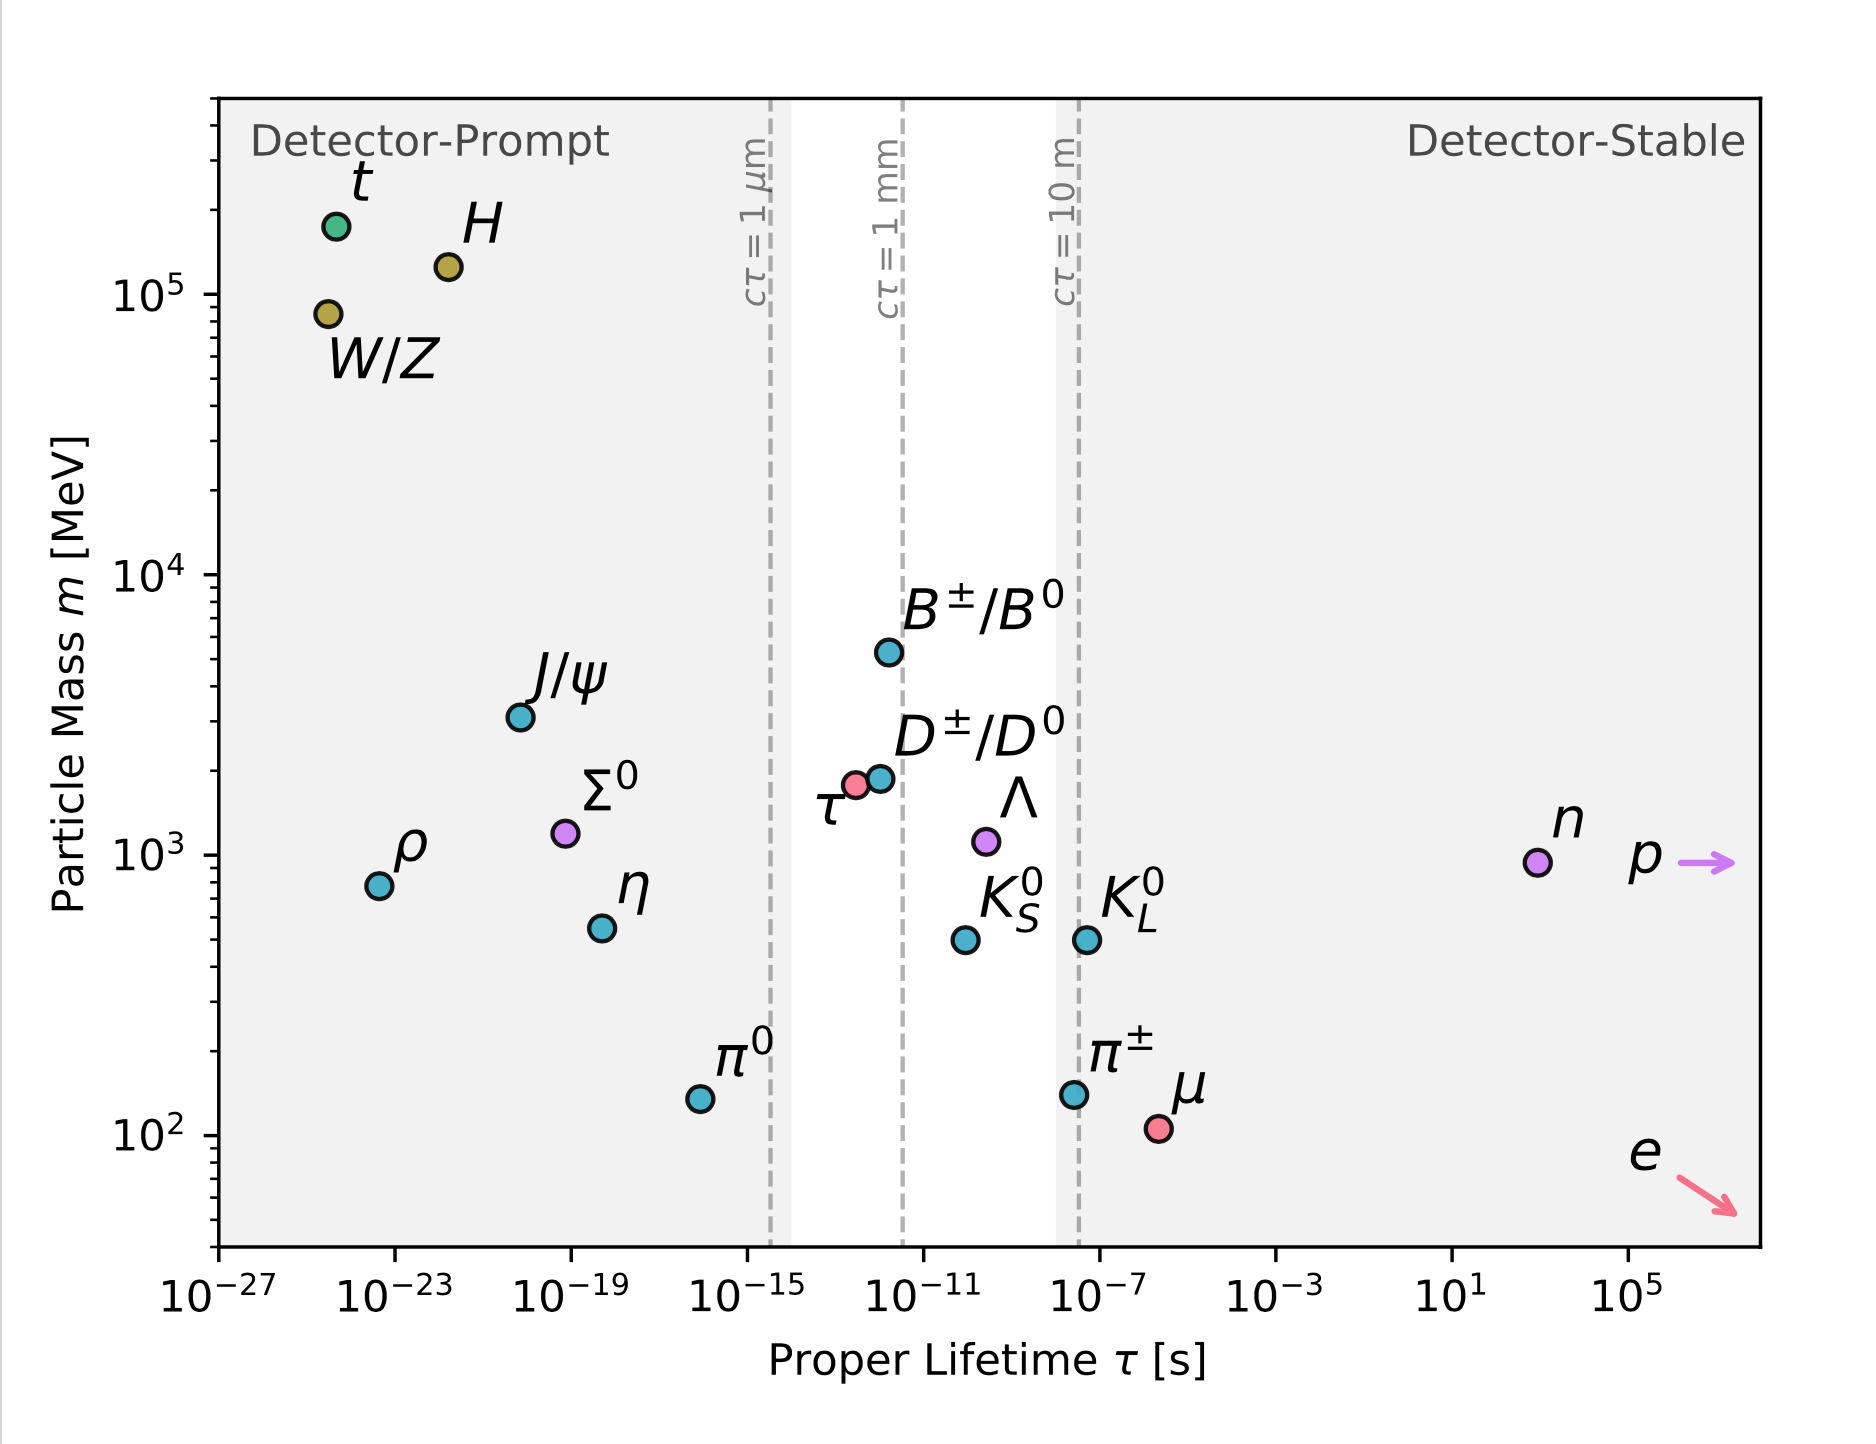
\includegraphics[width=.8\textwidth]{figures/theory/LLP-mass-lifetime.png}
\caption{A mass and proper lifetime distribution of particles in the \ac{SM}. There is a wide range of both masses and lifetimes. Shaded regions indicate detector-prompt or detector-stable particles. This assumes that particles traveling at the speed of light $\beta = 1$.}
\label{fig:llp-mass-lifetime}
\end{figure}

\section{Particle Decays}
%USED theory-LLP-Banerjee.pdf

The distance traveled by any relativistic particle can be described by

\begin{equation}
d = vt = \beta \gamma c t
\label{eq:sr_d}
\end{equation}

where $\gamma$ and $\beta$ have the usual special relativistic definitions: $\gamma = E/m = (1-\beta^2)^(-1/2)$, $\beta = v/c = |\vec{p}|/E$, $v$ is the particle's velocity, $t$ is the time the particle moves, and $c$ is the speed of light 

In the laboratory frame, the distance the particle travels before decaying is given by sending $t \rightarrow \tau$ in \autoref{eq:sr_d}, where $\tau$ denotes the proper lifetime of the particle measured in its own rest frame.

There is an exponential probability that the particle will decay at a given time ($t$) and location ($x$), given by 

\begin{equation}
P(x) = e ^{-x/(\beta \gamma \tau)}
\end{equation}

This means that even particles with large $\tau$ have a large probability at traveling very small distances before they decay, but particles with small $\tau$ cannot travel large distances before decaying. This fact is exploited to search for particles with large $\tau$, though the signature of the particle's decay in the detector varies greatly with the size of $\tau$. The relationship between decay radius and lifetime can be seen in \autoref{fig:d0-rltns}.


\section{\label{sec:llp-searches}Searches for Long Lived Particles}

\todo{need to hunt down papers and add references in the below}

\todo{Maybe add a doodle? Seperate doodles for each signature to just just copy heather's diagram?}

If more than one of the products of the \ac{LLP} decay are visible to the detector, one can look for its decay vertex. The \ac{LLP} will travel some distance from the \ac{PV}, where the particle is produced, and its decay vertex will be displaced, called a \ac{DV}. In this case, direct information about the lifetime of the particle can be deduced from the difference in distance between the \ac{LLP}'s prodcution and decay vertices (given by \autoref{eq:sr_d}). This vertices can appear in either tracking volume of the detector (\ac{ID} or \ac{MS}). There are many searches for \ac{DV}s in \ac{ATLAS}, many in conjunction with other physics objects related to the particlar theory model being probed. 

One can also directly search for the \ac{LLP}. In these cases, the \ac{LLP} is charged and leaves a peculiar track in the \ac{ID}. For example, one can look for highly ionizing tracks, indicating the presence of a massive particle that does not decay inside the \ac{ID} or for short tracks, where the decay products of the \ac{LLP} are not detected.

Finally, as in the case of this analysis, one can look for only the decay products of the \ac{LLP} by targetting  unconventionally presenting physics objects. For example, look for non-pointing photons in the \ac{LAr}, or emerging jets, which become visible midway through their hadronization. One can also look for displaced leptons, somewhat conventional lepton signtures that do not point back to the \ac{PV}. 

In these cases, it is often convenient to use \dzero, the transverse impact parameter, as a way to infer the lifetime of a particle. It does not give direct information about $\tau$, but decay products of particles with longer lifetimes have wider \dzero distributions as seen in \autoref{fig:d0-rltns}. In cases without a \ac{DV}, \dzero gives more precise information than any $R$ information realted to the track of the decay product. \dzero is calculated based on the shape of the track and has $\mathcal{0}(10)\mu \textrm{m}$ resolution (see \autoref{fig:trking_d0_res}). In $R$, we can only know the location of the first \ac{ID} layer associated to the track, with an $\mathcal{0}(10)\textrm{mm}$ resolution very sensitive to detector effects.

\todo{make a LLP decay diagram, also with different \pt}

\begin{figure}[htbp]
\centering
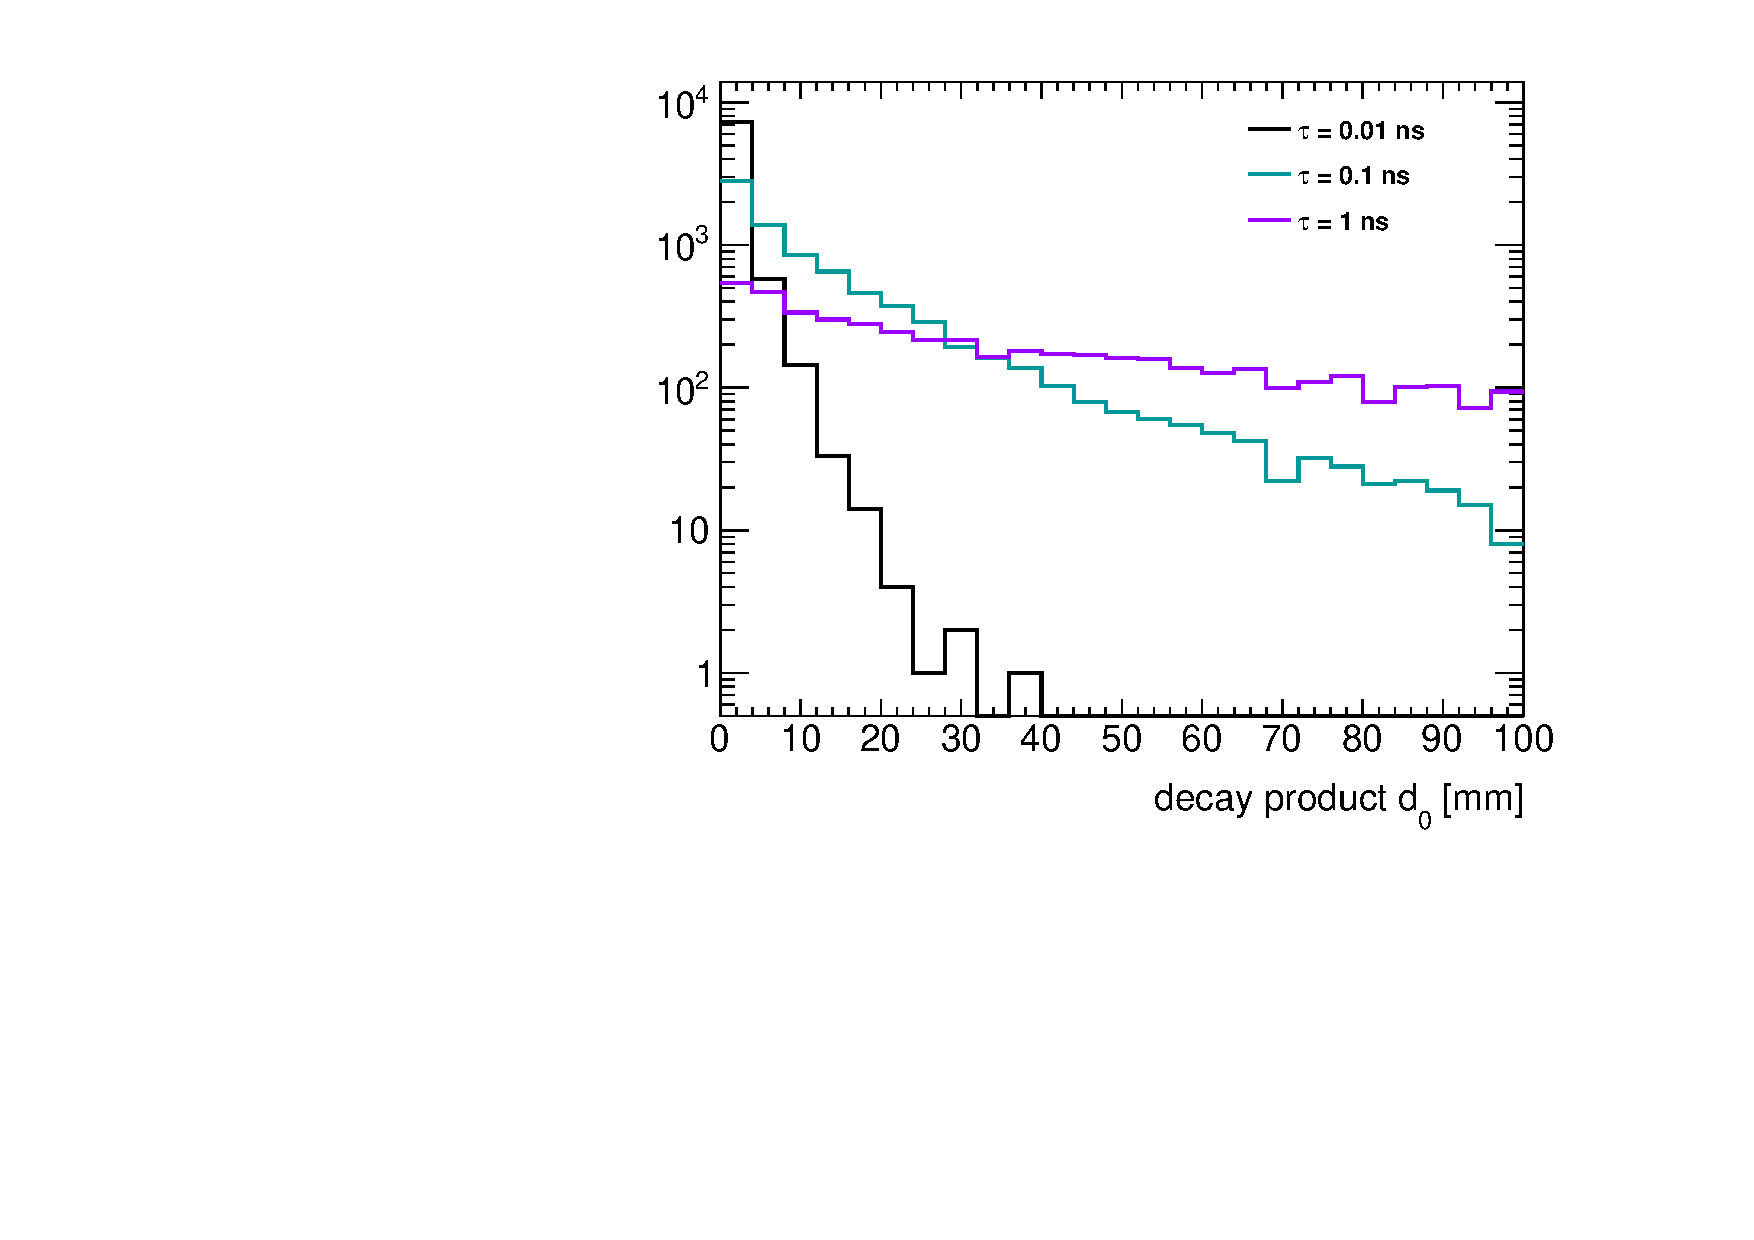
\includegraphics[width=.48\textwidth]{figures/theory/signal_d0.pdf}
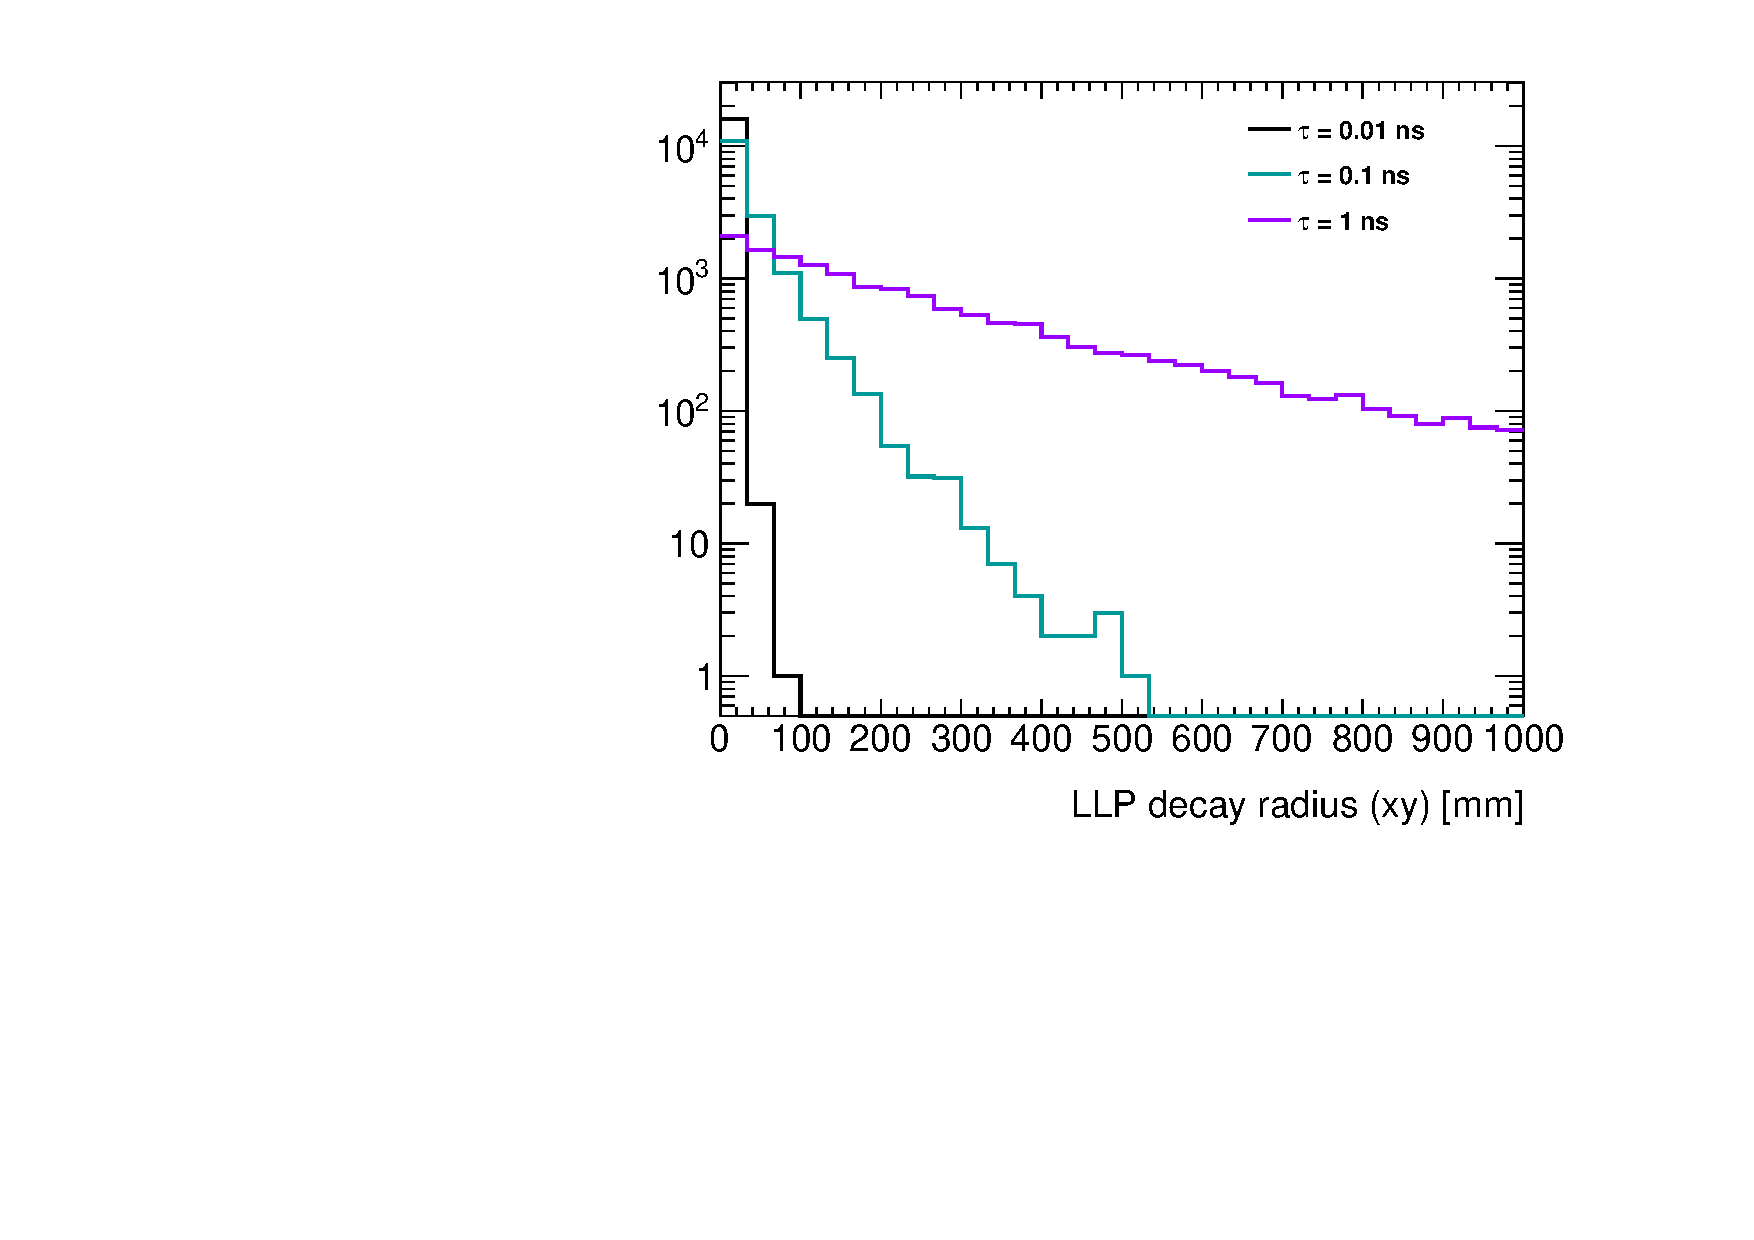
\includegraphics[width=.48\textwidth]{figures/theory/signal_rxy.pdf}
\caption{\dzero (left) and transverse decay radius ($x-y$) of \ac{LLP}s with different $\tau$. The left plot demonstrates that while \dzero does not directly give information about $\tau$, decay products of particles with longer lifetimes have wider \dzero distributions. These plots demonstrate only effects of the physical processes, not convolved with reconstrution effects.}
\label{fig:d0-rltns}
\end{figure}


These signatures are very unique with respect to other signatures searched for in \ac{ATLAS} which generally assume decay products originate at the \ac{PV}. These searches are dominated by \ac{SM} \emph{backgrounds}, physical phenomena that are not the target for measurement but have very similar signatures. \ac{LLP} searches generally have very little \ac{SM} background, but suffer from reconstruction challenges.A great deal of work is put into efficient and pure reconstruction and identification of unconventional physics objects.

Due to the technical challenges associated with \ac{LLP} searches, they are often done to be as \emph{model-independent} as possible. This means that, while there is usually a model to which a search brings unique sensitivity, the search not overoptimized for this model. For example, in this analysis, we target the displaced leptons; there are other objects in the targetting physical process, but we remain agnostic to them. Furthermore, the exponetial nature of the \ac{LLP} decay means that several searches, each targetting different signatures in different parts of the detector, are used in combination to explore the full lifetime phase space of a given model.






\cleardoublepage 

%----------------------------------------------------------------------------------------
\ctparttext{}
\part{Experiment}

\chapter{Particle Accelerators}

The world's largest machine is required to study the universe's smallest particles. The \ac{LHC} is circular particle collider located on the French-Swiss border outside of Geneva, Switzerland. A series of accelerators culminate in a $27$ km ring in which beams of hadrons, either protons or ions of heavier elements, are collided. There are four major experiments around the \ac{LHC} ring: \ac{ATLAS} and \ac{CMS}, general purpose detectors designed independently and with different priorities in order to serve as a cross-check for each other; \ac{ALICE}, a tracking-focused detector designed to study collisions of heavy ions; and \ac{LHCb}, an asymmetrical detector designed to study \ac{CP} violation. The \ac{LHC} has been running in its current form since 2008

The dataset used in this analysis comes from proton-proton, $pp$, collisions during Run 2 of the \ac{LHC}, which spanned from 2015-2018 and had a center of mass energy of $\sqrt{s} = 13 \TeV$.

\section{Accelerator Theory}

\todo{describe basics of beam: circle, bunches, IP}
\todo{describe magnets}

\subsection{Luminosity}

%USED pdg-review.pdf
If the primary goal of the collider is to study rare physics processes, whether difficult measurements of the \ac{SM} or heretofore unseen \ac{BSM} physics, enough data must be produced to be able to study them. The number of events of a given process in a given data set is given by

\begin{equation}
N_{\textrm{events}} = \mathcal{L}_{\textrm{int}} \times \sigma_{\textrm{process}}
\label{eq:nevents_lumi}
\end{equation}

where $\mathcal{L}$ is the \emph{integrated luminosity} of the dataset, and $\sigma_{\textrm{process}}$ is the cross section for the given process. More data ($\mathcal{L}_{\textrm{int}}$) is required to be able to see rare events (small $\sigma_{\textrm{process}}$), and many events are required in order to have the statistical power in able to make a discovery. The integrated luminosity is the integral of the instantaneous luminosity over data taking time

\begin{equation}
\mathcal{L}_{\textrm{int}} = \int \mathcal{L} dt
\end{equation}

and the \emph{instantaneous luminosity} is related to the parameters of the accelerator. For two identical bunches with $N_1$ and $N_2$ protons per bunch colliding with frequency $f$:

\begin{equation}
\mathcal{L} = \frac{N_1 N_2 f}{4\pi \sigma_x^* \sigma_y^*} \mathcal{F}
\end{equation}


where $\sigma_x^*$ and  $\sigma_y^*$ are the \ac{rms} of the beam width in the $x$ and $y$ directions, and $\mathcal{F}$ is a factor that takes in other geometric effects such as the crossing angle and bunch length, it is generally $\mathcal{O}(1)$. It can be rewritten more specifically for the \ac{LHC} as

\begin{equation}
\mathcal{L} = \frac{N_b^2 n_b f }{4\pi \sqrt{\epsilon_n \beta^*_x \beta^*_y}}\mathcal{F}
\end{equation}

Where $N_b$ is the number of protons per bunch (assuming $N_1 = N_2$), $n_b$ is the number of bunches in the beam, $\epsilon_n$ is the \emph{emittance}, which describes the spread of the particles in the bunch, and $\beta^*$ is the value of the $\beta$-function at the \ac{IP}. The $\beta$-function describes the size of the beam as a function of location. A sampling of the values of these parameters in 2018 are shown in \autoref{tab:lumi-vals}.


%USED ATLAS-lumi-measurement.pdf
\begin{table}
\centering
\begin{tabular}{lc}
\hline
Paramter & value  \\
\hline
$N_b$ (protons per bunch)                                           & $1.1 \times 10^{11}$   \\
$n_b$ (bunches per beam)                                            & $2544$   \\
$\beta^*$ (beam size)                                               & $.3$ m   \\
$\epsilon_n$ (beam spread)                                          & $3 \mu$m-radians   \\
$\mathcal{L}_{\textrm{peak}}$ (peak instantaneous luminosity)       & $21 \times 10^{33} \textrm{cm}^{-2}\textrm{s}^{-1}$   \\
space between bunches                                               & $25$ ns   \\
\hline
\end{tabular}
\caption{Beam parameters for 2018 for standard running conditions used in the data collection for this analysis. Special runs take place where these parameters are changed.}
\label{tab:lumi-vals}
\end{table}

Several of these factors can be manipulated \emph{in situ}, allowing for luminosity increasing or decreasing, depending on the need. Decreasing $\beta^*$ increases the luminosity, so the beams are \emph{squeezed} with focusing quadrupole magnets at the \ac{IP}. Nonzero beam crossing angles and longer bunches decrease $\mathcal{L}$. In fact, during some runs of Run 2 of the \ac{LHC}, the beam angle was changed at the beginning in order to decrease the luminosity to a level more tolerable by the experiments, referred to as \emph{leveling}. 

The instantaneous luminosity can be measured by measuring the components directly, or it can be inferred by measuring the number of events in a process with a well measured cross section, $\sigma_{\textrm{ref}}$ that produces $N_{\textrm{ref}}$ events. By counting $N_{\textrm{exp}}$, the actual number of events produced, one can infer $\sigma_{\textrm{exp}}$. The difference between $\sigma_{\textrm{ref}}$ and $\sigma_{\textrm{exp}}$ gives information about the instantaneous luminosity from an equation similar to \autoref{eq:nevents_lumi}. It is measured in units of $\textrm{cm}^{-2}\textrm{s}^{-1}$ and after integration over time, the integrated luminosity is measured in inverse \emph{barns}. Where $1 b = 10^{-28} \textrm{m}$. This simplifies the $N_{\textrm{events}}$ calculation in \autoref{eq:nevents_lumi} where the cross section is also measured in barns.


\todo{is this how it's done in ATLAS? see ATLAS-lumi-measurement.pdf}


In Run2, the \ac{LHC} produced an integrated luminosity of $156 \textrm{fb}^{-1}$, \ac{ATLAS} recorded $147 \textrm{fb}^{-1}$, with $139 \textrm{fb}^{-1}$ available to be used for physics analyses.




\section{The Large Hadron Collider}
\todo{steps of injecting}

\subsection{Pileup}


\chapter{The ATLAS Detector}

The \ac{ATLAS} detector is a cylindrical general purpose particle detector designed to measure the products of $\sqrt{s} = 14 \TeV$ proton-proton collisions at the \ac{LHC}. It consists of three major sub-detectors: closest to the beamline is the the \ac{ID}, which measures the trajectories of charge particles, followed by the Calorimeters, which measure the energies of electromagnetic and hadronically interacting particles, and finally the \ac{MS} which measures the trajectories of muons. The \ac{ID} is surrounded by a super conducting solenoidal magnet that provides a uniform $2$T magnetic field, enabling measurement of particles' charge and momentum, and a toroidal magnet surrounds \ac{MS}, allowing for charge and momentum measurements of muons. In general, each subdetector consists of a barrel detector parallel to the beampipe and end-cap detectors perpendicular to the beampipe. \cite{atlas-overview}

A schematic of the \ac{ATLAS} detector is shown in \autoref{fig:atlas-schematic}.


%https://atlas.cern/discover/detector
\begin{figure}[htbp]
\centering
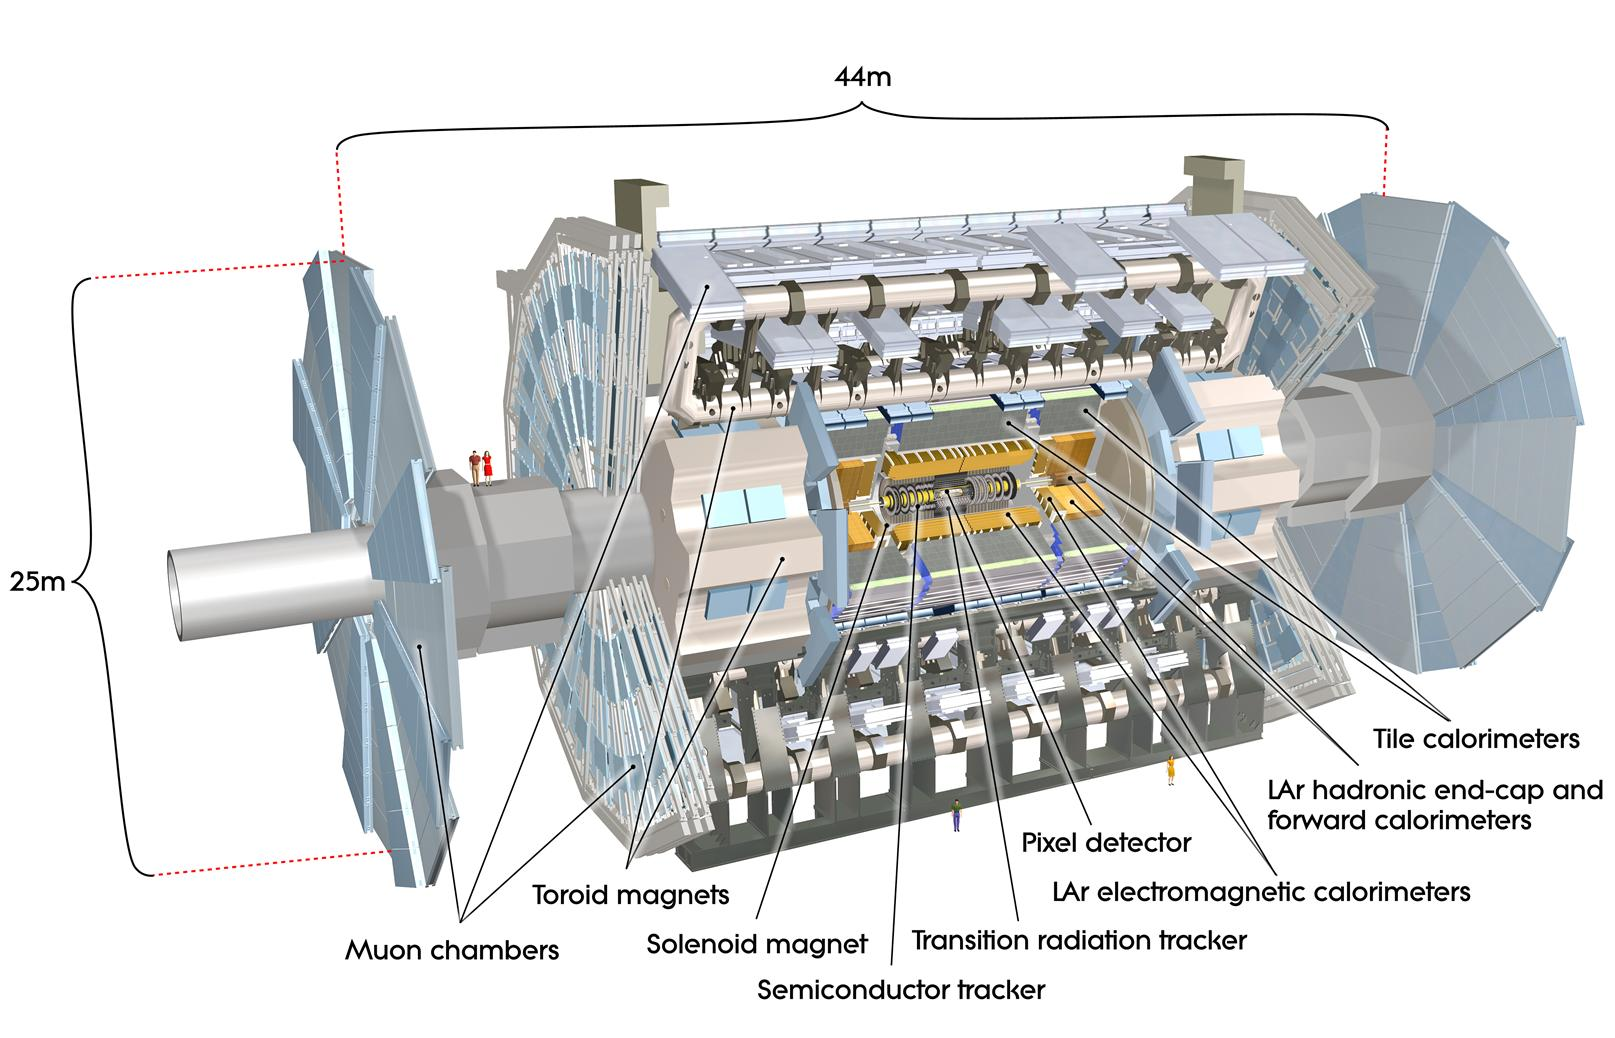
\includegraphics[width=.8\textwidth]{figures/Detector/atlas-schematic.jpg}
\caption{A diagram of the \ac{ATLAS} detector. The dimensions, subdetectors, and magnet systems are labeled. }
\label{fig:atlas-schematic}
\end{figure}

\section{Coordinate System}
\ac{ATLAS} uses a Cartesian right-handed coordinate system, with the origin defined as the $pp$ collision point. The $z$-axis points along the beampipe, where $+z$ points counter-clockwise. The transverse plane, the $y$-axis and $x$-axis, points upward and toward the center of the \ac{LHC} ring, respectively. The detector is built with with symmetry across the origin in in $z$, as well as with rotational symmetry in the transverse plane. The $+z$ side of the detector is referred to as the A-side, and $-z$ as the C-side.

Cylindrical coordinates provide a comfortable description of the \ac{ATLAS} detector, where $\phi$ measures the angle in the $x-y$ plane around the beampipe, and $\theta$ the angle from the $z$ axis. $\phi$ is positive for positive $y$. 

A given particle's momentum in $z$ is not known, but its transverse momentum is known to be $0$, so it is advantageous to define spatial variables independent of $z$ momentum. Thus, instead of $\theta$, $\eta = - \textrm{ln}(\textrm{tan}\frac{\theta}{2})$ is used to describe angle from the $z$ axis. Particles perpendicular to the $z$ axis have $\eta = 0$, while those parallel to the beamline have $\eta \rightarrow \infty$. 

Angular distances between objects is described using $\Delta R = \sqrt{\Delta \eta ^2 + \Delta \phi ^2}$ and the radial distance from the origin in the $x-y$ plane is denoted $R$. 

A particle's momentum will generally be described in terms of its \pT, its momentum in the transverse direction. A particle's $3$-vector is described by $(\pt, \eta, \phi)$, which are all invariant under boosts in $z$ assuming the particle can be considered massless (which is true in the case of particles in \ac{ATLAS}).





%USED ATLAS-overview.pdf
\section{Inner Detector}
The Inner Detector measures the trajectories of charged particles resulting from \ac{LHC} collisions. The \ac{ID} covers the region with $|\eta| < 2.5$, measuring approximately $1000$ particles per bunch crossing. In order to achieve the momentum and vertex resolution required to achieve \ac{ATLAS}'s physics goals three subdetectors are used: the Pixel detector, the \ac{SCT}, and the \ac{TRT}. The Pixel and \ac{SCT} detectors are used for high granularity precision tracking and the \ac{TRT} is used to distinguish electrons from converted photons. All of this is immersed in a $2$T magnetic field, curving charged particles in proportion to its momentum in the $\phi$ direction.

\todo{describe conversions somewhere... Maybe in particle descriptions in theory?}


The \pt resolution of the \ac{ID} scales with track \pt. Higher \pt tracks are less curved, so the measurement resolution is worse. In the \ac{ATLAS} \ac{ID}, the \pt resolution  $0.05\% \times \pt$ with a $1\%$ constant term. The constant term describes measurement uncertainties that do not scale with momentum or energy, such as material imperfections, non-uniform detector response, or other constant measurement issues and is added in quadrature ($\oplus$) with the stochastic term.

The combination of thre three trackers with radii ranging from 32.33 mm to 1082mm enable robust and precise pattern recognition. The Pixel detector enables secondary vertex measurements, and combined with the \ac{SCT} enables impact parameter measurement and vertexing for heavy-flavor jet and $\tau$-lepton tagging. the The \ac{TRT} has lower precision per point, but measures a longer track and contributes signficantly to the momentum measurement.


A schematic of the \ac{ID} can be seen in \autoref{fig:atlas-id} and a detailed distribution of the various subdetectors is shown in \autoref{fig:atlas-id-layers}. 


%https://cds.cern.ch/images/CERN-GE-0803014-01/file?size=medium
\begin{figure}[htbp]
\centering
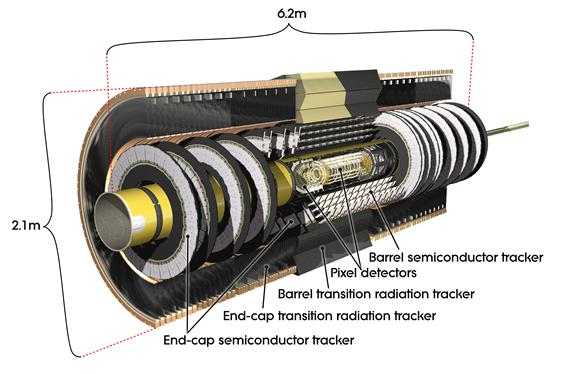
\includegraphics[width=.8\textwidth]{figures/Detector/atlas-ID.jpg}
\caption{A diagram of the \ac{ATLAS} \ac{ID} with the major subsystems labeled. The Pixel and \ac{SCT} are of particular importance for this analysis.}
\label{fig:atlas-id}
\end{figure}

%https://www.researchgate.net/publication/325643426/figure/fig8/AS:669532737769482@1536640452588/Segment-of-the-ATLAS-inner-detector-showing-the-tracker-layers-The-silicon-strip.ppm
\begin{figure}[htbp]
\centering
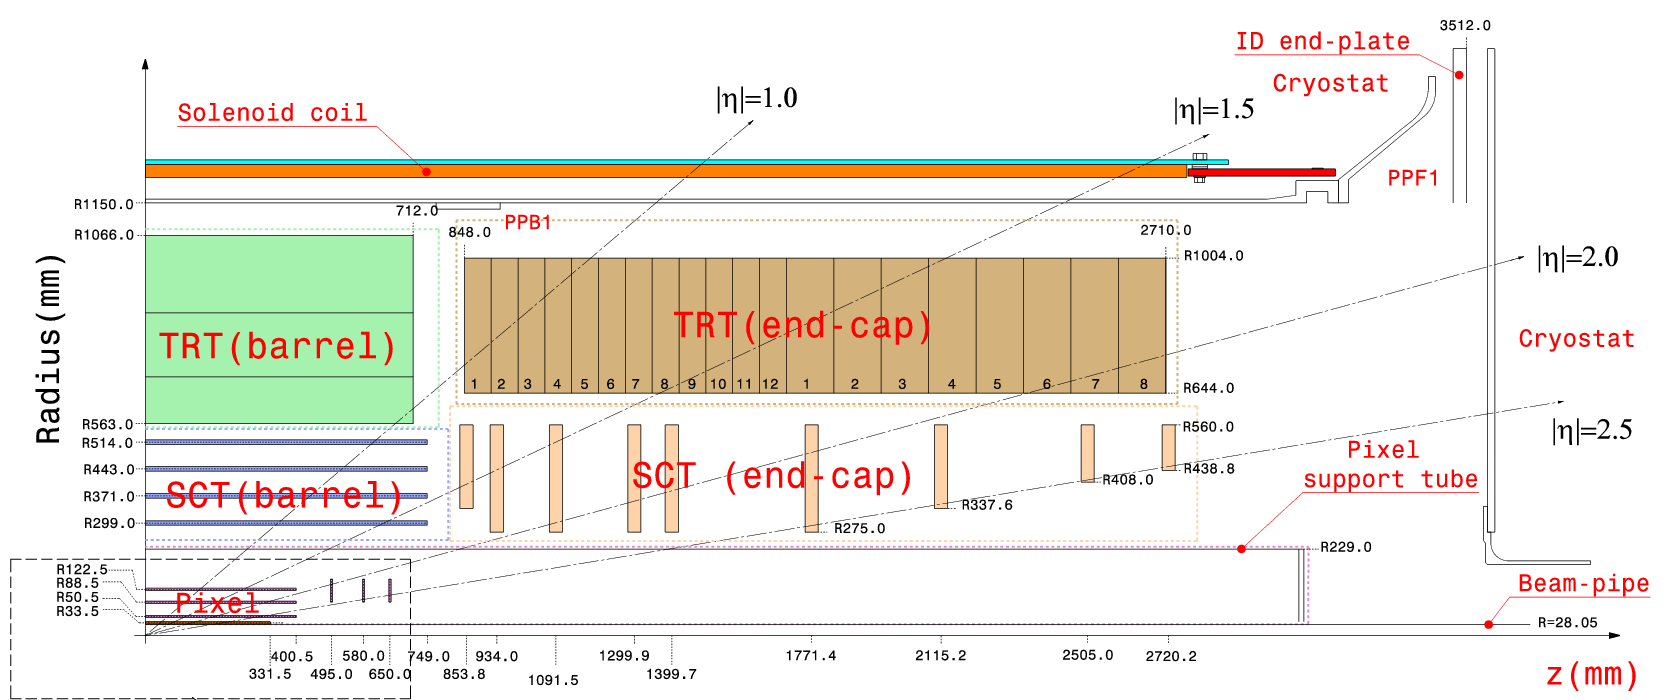
\includegraphics[width=.8\textwidth]{figures/Detector/atlas-id-layers.png}
\caption{A schematic of the \ac{ATLAS} \ac{ID} shown in the $R-z$ plane. \cite{id-cutaway}}
\label{fig:atlas-id-layers}
\end{figure}

\subsection{Silicon Detectors}



\subsection{The Pixel Detector}

The Pixel detector is the closest one to the beam and have the highest granularity. The pixels are arranged parallel to the beam axis in concentric cylindrical layers in the barrel and perpendicular to the beam axis on disks in the endcap regions. The current Pixel detector consists of the Run 1 detector with the \ac{IBL} installed closed to the beam pipe. 

The Run 1 Pixel detector has 3 concentric cylindrical layers in the barrel and 3 disks in the endcap. It is composed of 1744 pixel sensors, each with 47232 pixels. Each pixel is identical has minimum size of $R-\phi \times z = 50 \times 400 \mu \textrm{m}^{2}$ (increasing to $R-\phi \times z = 50 \times 600 \mu \textrm{m}^{2}$ near a front-end chip). In the barrel, they have accuracy of $10 \mu \textrm{m}$ in $R-\phi$ and $115 \mu \textrm{m}$ in $z$, and in the endcaps they have accuracy of $10 \mu \textrm{m}$ in $R-\phi$ and $115 \mu \textrm{m}$ in $R$ and the detector has 80.4 million pixels and readout channels. 

The \ac{IBL} is the inner most Pixel layer installed for Run 2 33.2 mm away from a new, narrower beampipe. A closer detector layer enables better impact parameter resolution as well as providing extra radiation shielding for the former closest Pixel layer (called the B-layer). The \ac{IBL} is composed of 12 million smaller pixels, $R-\phi \times z = 50 \times 250 \mu \textrm{m}^{2}$, assembled on 14 staves, with a resolution of $8 \mu\textrm{m}$ in $R-\phi$ and $40 \mu\textrm{m}$.

The two innermost detectors, the Pixel and \ac{SCT} detectors, are made of silicon, the preferred tracking medium of particle physics detectors. The \ac{ATLAS} pixels are n-type semiconductors (impurities have been added to increase the number of potential electron charge carriers) with a voltage applied (150-600V in the Pixel detector).  When a charged particle interacts with a silicon detector layer, electron-hole pairs are created and these pairs drift toward the readout chips in the magnetic field. If enough of these pairs are created such that the signal becomes greater than a pre-specified noise threshold, the signal is readout as a \emph{hit}. A particle must have 3.6 eV to induce about 80 electron-hole pairs per $\mu$m. Pixels provide a high signal-to-noise ratio, and so are preferred in regions where high occupancy is possible (such as close to the beamline). \cite{silicon} 

\subsection{The Silicon Microstrip Tracker}
A particle moving through the \ac{SCT} crosses 4 bilayers of the detector creating 4 hit measurements as it interacts with 8 layers of material. In the barrel, each bilayer is composed of 2 stereostrips, one parallel to the beam axis (measuring $R-\phi$) and the other rotated by 40 mrad. The combination of the stereostrips in the bilayer gives a 3-dimensional measurement. In the end caps, the bilayers are arranged on 9  disks per side such that the second layer is offset 40mrad from a radial strip. The strips are 12cm long and $80 \mu\textrm{m}$ thick.

Less precise than the Pixels, in the barrel region, they have accuracy of $17 \mu \textrm{m}$ in $R-\phi$ and $580 \mu \textrm{m}$ in $z$, and in the endcaps they have resolution of $17 \mu \textrm{m}$ in $R-\phi$ and $580 \mu \textrm{m}$ in $R$. The use of strips instead of pixels reduces the number of readout channels as well as the cost: there are 15192 sensors each with 768 strips with an applied voltage of 150-300V and 6.3 million readout channels 
 

\subsection{The Transition Radiation Tracker}
The \ac{TRT} is straw-tube tracker that extends the tracking volume by almost 500 mm without the cost of that much additional silicon. The tubes have a diameter of 4mm and made of Kapton and carbon fibers. They are filled with a gas mixture (70\% Xe, 27\% CO$_{2}$, and 3\% O$_{2}$) and a 31 $\mu$m diameter gold-plated tungsten wire. The wires are divided into two halves about $\eta = 0$. In the barrel, 52 544 straws are parallel to the beam axis and 144 cm long. In the endcaps, 122 880 37 cm long straws are arranged radially in wheels. The \ac{TRT} has 351,000 readout channels.

When a charged particle passes through the tube, the gas is ionized and the resulting free electrons drift toward the wire where they are amplified then readout. A particle passing through the \ac{TRT} typically leaves 36 hits. The \ac{TRT} only provides $R-\phi$ measurements with an accuracy of $130 \mu\textrm{m}$ per straw. However, its length improves measured momentum resolution and it also can provide ns-level timing information.


\subsection{Solenoid Magnet}

The central solenoid surrounds the \ac{ID} and provides a uniform $2\textrm{T}$ field that bends the trajectories of charged particles. The transverse momentum of the particle can be inferred from its radius of curvature, $R$, in the $x-y$ plane using the equation $p_{T} = qBR$, where $q$ is the charge of the particle and $B$ the magnetic field in the $z$ direction.

However, the placement of the solenoid between the \ac{ID} and calorimeters necessitates careful design choices so that all of a given particle's energy is still measured by the calorimeters. The solenoid only contributes about $0.66$ radiation lengths \footnote{Radiation lengths measure the mean distance in which an electron loses all but $\frac{1}{e}$ of its energy.}. In order to achieve this, the solenoid and \ac{EM} calorimeter share a vacuum vessel, eliminating the need for two vacuum walls. It is made of Al-stabilised NbTi superconductor which allows a high electric field to be achieved ($7.730 \textrm{kA}$) while optimizing the thickness of the coil. The solenoid has an axial length of $5.8 \textrm{m}$ and radial thickness of $100 \textrm{cm}$ and it operates at a temperature of $4.5 \textrm{K}$. 


\section{Calorimeters}

The \ac{ATLAS} calorimeters measure the energy of electromagnetic and hadronic particles. The calorimeter system is composed of \ac{EM}, hadronic, and forward calorimeters. While they use a variety of different technologies to measure energies, they are both sampling calorimeters composed of alternating active and absorbing layers. Particles shower in absorbing layers and the showers are measured in the active layers, but the actual energy of each particle is not measured because some is lost to the absorbing layers. Unlike the tracker, the energy resolution of a calorimeter increases with increasing energy due to the increased signal generated. The size of each calorimeter is set by its radiation length or nuclear interaction length such that the calorimeter absorbs all of given particle's energy by the far end of the calorimeter and only muons and neutrinos should escape the calorimeters layers. A schematic of the \ac{ATLAS} calorimeters can be seen in \autoref{fig:atlas-calos}


%https://arxiv.org/pdf/1603.02934.pdf
\begin{figure}[htbp]
\centering
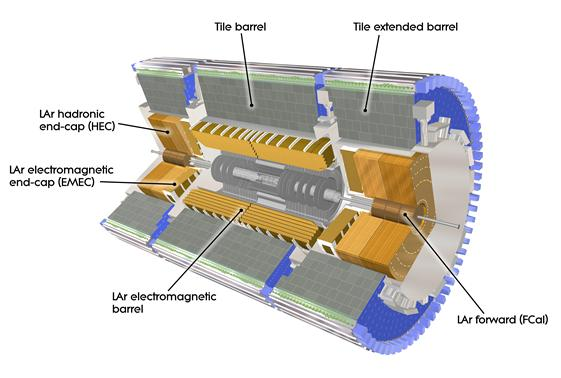
\includegraphics[width=.8\textwidth]{figures/Detector/atlas-calorimeters.jpg}
\caption{A diagram of the \ac{ATLAS} calorimeters with the major subsystems labeled. The \ac{EM} calorimeter is of particular importance for this analysis. \cite{calorimeters}}
\label{fig:atlas-calos}
\end{figure}


\subsection{Electromagnetic Calorimeter}

The \ac{LAr} \ac{EM} calorimeter is the innermost calorimeter and gives excellent energy and position resolution. \cite{calorimeters} It is composed of barrel ($|\eta| < 1.5$) and end-cap ($1.4 < |\eta| < 3.2$) components. Both components use a lead absorber with liquid argon active material. The layers of the calorimeter have an accordion shape (shown in \autoref{fig:atlas-lar}), which allows for the multiple absorbing layers without any gaps between them, as well as complete $\phi$ symmetry. The first layer has finer segmentation in $\eta$ to allow for more precise angular measurements of photons (which do not produce an \ac{ID} track). The thickness of the absorbing plates varies as a function of $\eta$ to optimize energy resolution. An active liquid argon presampler is placed before the accordion layers in the region with $|\eta| < 1.8$ to correct for energy loss upstream of the calorimeter. It is about 22 radiation lengths wide and gives energy resolution of $10\%/\sqrt{E} \oplus 0.7\%$

%https://www.researchgate.net/profile/Denis_Oliveira_Damazio/publication/229849719/figure/fig2/AS:667635272413188@1536188061121/Calorimeter-cells-for-different-layers-left-Note-the-very-fine-segmentation-in-the_Q320.jpg
\begin{figure}[htbp]
\centering
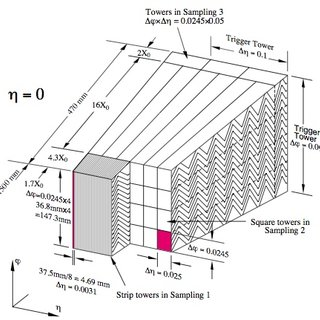
\includegraphics[width=.6\textwidth]{figures/Detector/lar.jpg}
\caption{A diagram of the \ac{ATLAS} \ac{EM} \ac{LAr} calorimeter. It has a unique shape in order to provide precision position and energy resolution.}
\label{fig:atlas-lar}
\end{figure}


\subsection{Hadronic Calorimeter}

The hadronic calorimeter surrounds the \ac{EM} calorimeter also within $|\eta| < 3.2$. The barrel region ($|\eta| < 1.7$) is made of steel absorbers with active material of scintillating tiles. Here, the calorimeter is about $2$m long in the radial direction and covers about $8$ interaction lengths. The Hadronic End-cap Calorimeters cover the region $1.5 < |\eta| < 3.2$ with a copper absorber and liquid argon active material.


The hadronic calorimeter has an energy resolution of  $50\%/\sqrt{E} \oplus 3\%$. 

\subsection{Forward Calorimeter}
The \ac{FCAL} is measures  both \ac{EM} and hadronic energy and extends coverage to $3.1 < |\eta| < 4.9$. The detector uses liquid argon as its active material with copper (for \ac{EM} activity) and tungsten (for hadronic activity) absorbers. It is about $10$ interaction lengths deep and also serves to add some shielding to the \ac{MS}. The energy resolution of the \ac{FCAL} is $100\%/\sqrt{E} \oplus 10\%$.




\section{Muon Spectrometer}
The Muon Spectrometer is the outermost subdetector designed to detect muons, which are too massive to be stopped by the calorimeters, and measure their momentum. This is achieved using a toroidal magnet system that deflects muons as they pass through through  high-precision tracking chambers and separate chambers used for triggering. The magnetic field points in the $\eta$ direction, orthogonal to the muon's direction of motion, and the detector as well as the toroid system is symmetric in $\phi$.

The \ac{MS} can measure muons with $|\eta| < 2.4$ and $3 \GeV < {\pt}_{\mu} < 10 \TeV$. The main performance goal is to provide a stand-alone (independent of the \ac{ID}) momentum resolution of $10\%$ at $\pT > 1 \TeV$; a particle moving with $\pt = 1 \TeV$ has a \emph{sagitta} (see \autoref{fig:ms-sagitta}) of $500\mu\textrm{m}$ that needs to be measured with a resolution of $<50\mu\textrm{m}$. Even at 3 \TeV, the \ac{MS} has good momentum resolution and is still able identify the charge of the particle based on its bending direction. Furthermore, the triggering chambers have timing resolution of $1.5-4 \textrm{ns}$.  

\ac{MDT}s are used for precision tracking in the $\eta$ coordinate in the range $|\eta| < 2.7$, except in the inner most layer where the \ac{MDT}s extend only to $|\eta| < 2.0$ and \ac{CSC}s cover the region $2.0|\eta| < 2.7$. Triggering and $\phi$ measurements are provided by \ac{RPC}s in the range $|\eta| < 1.05$ and \ac{TGC}s in $1.05 |\eta| < 2.7$. A schematic of the \ac{MS} can be seen in \autoref{fig:atlas-ms}.  

\todo{Describe MDTs}

While the \ac{MDT}s give extremely precise measurements of muon directions, they cannot be used in isolation for the physics goals of \ac{ATLAS}. First, they are finely segmented in $\eta$, the bending direction of the muons, enabling the high momentum resolution. However, in $\phi$, their resolution is as good as the length of the tube, several meters long. Additionally, being drift tubes, their readout is very slow and cannot be used in the quick response time required for triggering. Thus, \ac{RPC}s (in the barrel) and \ac{TGC}s (in the endcaps) complement the \ac{MDT}s for triggering and \ac{CSC}s complement the \ac{MDT}s in the forward region (where the particle incident rate is the highest) to provide better 2-dimensional position measurements. A comparison of the resolution of the relevant parameters is seen in \autoref{tab:ms-parts}/
\todo{include description of MS timing}

\begin{table}[htb]
\begin{center}
\begin{tabular}{ccccc}
Detector    & function & z/R resolution & $\phi$ resolution & time resolution \\
 \hline
  \ac{MDT}  &  tracking   &  35\um (z)  & 2.5-5 m  & $<$ 700 ns \\
  \ac{CSC}  &  tracking   &  30 \um(R)  & 5 mm     & 7 ns   \\
  \ac{RPC}  &  triggering &  10 mm (z)  & 10 mm    & 1.5 ns  \\
  \ac{TGC}  &  triggering &  2-6 mm (R) & 3-7 mm   & 4 ns  \\
\hline
\end{tabular}
\caption{Resolutions of the various parts of the \ac{MS}. The endcap detectors (\ac{CSC}s and \ac{TGC}s) give resolution in R while the barrel detectors (\ac{MDT}s and \ac{RPC}s) give resolution in z. The various pieces of the \ac{MS} enable 2 dimensional precision measurement as well as measurements to be used in the trigger.}
\label{tab:ms-parts}
\end{center}
\end{table}


The \ac{CSC}s are multiwire proportional chambers with anode wires oriented radially. One of the  cathodes is segmented with strips perpendicular to the wires giving a precision measurement in the bending plane ($\eta$) of with resolution of 40\um and the other segmented parallel to the wire, giving a transverse ($\phi$) measurement with 5mm resolution.  

\begin{figure}[htbp]
\centering
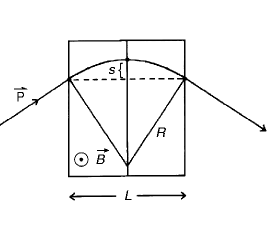
\includegraphics[width=.6\textwidth]{figures/Detector/ms-sagitta.png}
\caption{The trajectory of a particle in a magnetic field (``B''). The particle's sagitta, labeled ``s'' is the bending distance in the direction perpendicular to the magnetic field. The direction of the bending is dictated by the charge of the particle. The higher the momentum of a particle, the smaller the sagitta. \cite{particledetectors-springer}}
\label{fig:ms-sagitta}
\end{figure}


%$https://cds.cern.ch/record/1631701/files/MuonSpectrometer_profile.png
\begin{figure}[htbp]
\centering
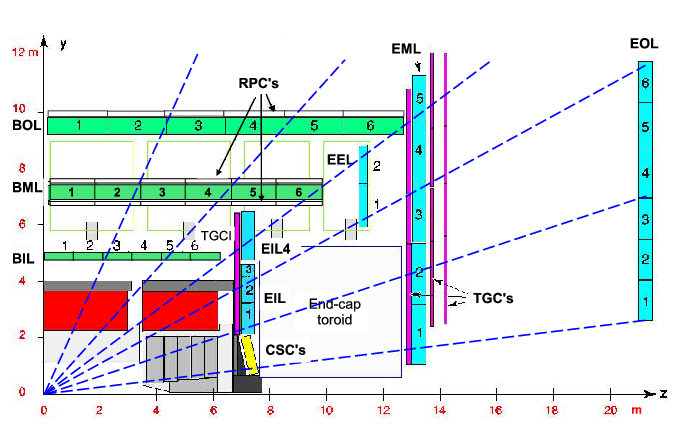
\includegraphics[width=.8\textwidth]{figures/Detector/atlas-ms.png}
\caption{A diagram of the \ac{ATLAS} \ac{MS} in the $r-z$ plane. The barrel \ac{MDT} are shown in green and the \ac{RPC} shown in black. In the end-caps, the \ac{MDT} are shown in blue and the \ac{TGC} shown in purple. \cite{ms-vertices}}
\label{fig:atlas-ms}
\end{figure}






\begin{figure}[htbp]
\centering
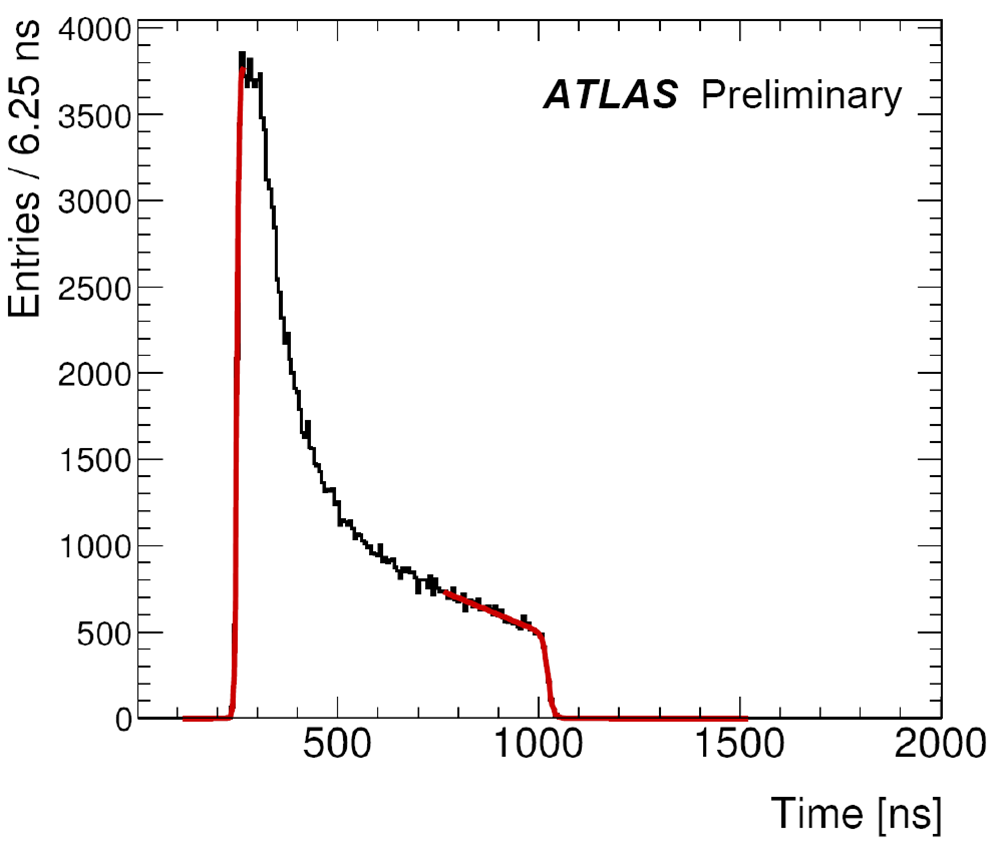
\includegraphics[width=.8\textwidth]{figures/Detector/mdt-t0.png}
\caption{A distribution of \ac{MDT} time measurements. The $t_{0}$ is the time between 0 and the peak of the distribution, shown by the leftmost red line. The rightmost red line indicates $t_{\textrm{max}}$, the end of the \ac{MDT} signal.}
\label{fig:ms-t0fit}
\end{figure}





\subsection{Toroid Magnets}

The toroid magnet system, composed of a barrel and two end-caps, provides a toroidal magnetic field of $0.5 \textrm{T}$ and $1 \textrm{T}$ for the barrel ($|\eta| < 1.4$) and end-cap ($1.6 <|\eta| < 2.7$) regions of the \ac{MS} (in the transition region ($1.5 < |\eta| < 1.6$) muons are bent by a combination of the two fields). The toroid is much larger than the solenoid, $25.3 \textrm{m}$ long and $10 \textrm{m}$ in radial width, but also operates at a temperature of $4.5 \textrm{K}$. All three toroid magnets are made of Al-stabilized Nb/Ti/Cu conductor. They have an air-core structure, which gives them a strong bending power over a large volume while minimizing additional material scattering. 




\section{Particles in ATLAS}
The previously described subdetectors are used in combination to identify particles in \ac{ATLAS}. Charged particles interact with the \ac{ID} resulting in hits to be reconstructed into tracks. A track that points to a calorimeter cluster indicates the kind of charged particle that made the track and a cluster without an associated track indicates a neutral particle. The calorimeters are designed such that they absorb all of the energy of a particle and \ac{EM} particles do not enter the hadronic calorimeter, and hadronic particles do not enter the \ac{MS}. Muons do not interact with the calorimeters, but do leave a track in both the \ac{ID} and \ac{MS}. The only \ac{SM} particle that escapes the detector entirely is a neutrino. An undetected particle, like an \ac{SM} $\nu$ or some \ac{BSM} particle, could be seen as an imbalance in transverse momentum. The transverse momenta of all particles should sum to zero in order to conserve momentum, so any non-zero sum indicates an undetected particle.


\begin{figure}[htbp]
\centering
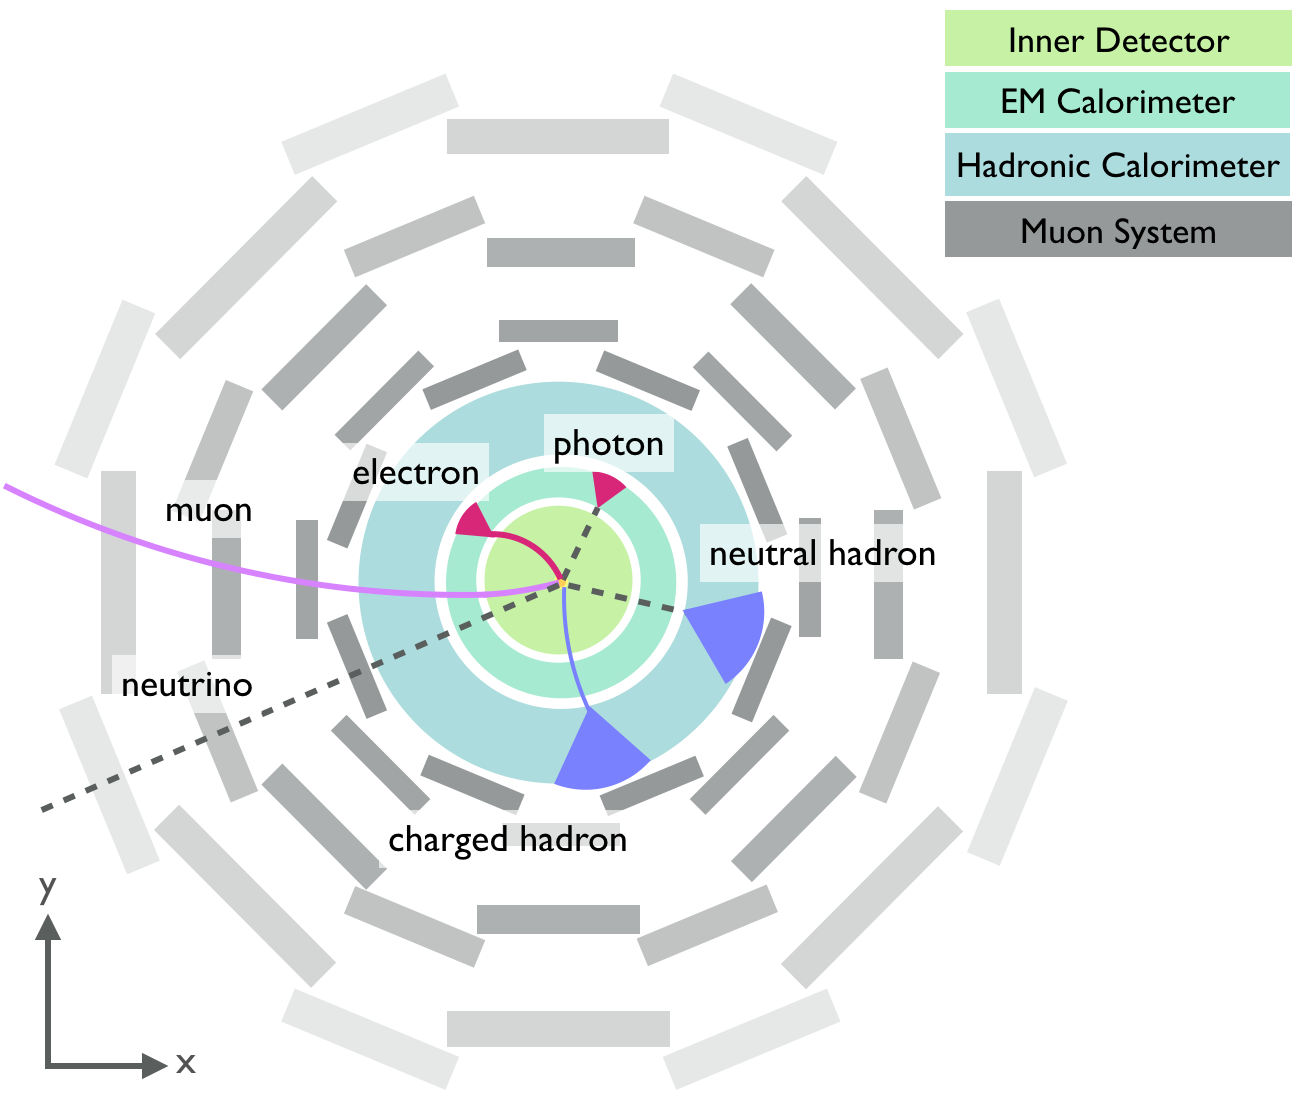
\includegraphics[width=.8\textwidth]{figures/Detector/particle-doodle.png}
\caption{A schematic of the signatures of Standard Model particles in the \ac{ATLAS} detector that illustrates how the subdetectors are used together to identify particles. Dashed lines indicate a particle trajectory that leaves no detector signature. Figure not drawn to scale nor does it represent a real physical process.}
\label{fig:particle-doodles}
\end{figure}





\chapter{Data Acquisition}

\section{Overview}
\section{General Challenges}
\section{Challenges for Long Lived Particles}
\section{The Fast TracKer}
\section{Fast TracKer Applications for Long Lived Particles and Future Prospects}

\chapter{Event Reconstruction}
\label{ch:EventReconstruction}

Event reconstruction is the process by which detector signals are converted into objects that can be used for physics analysis. This is a complex process that requires a great deal of focused effort by the \ac{ATLAS} collaboration. First, digital signals from the detector are collected into tracks and clusters, then they are combined to form reconstruction-level physics objects. Then, a identification steps is performed, where quality requirements are placed on the reconstruction-level objects to identify them as signatures of physical particles, like electrons and muons, that can be used in physics analyses. 

These algorithms are centrally developed by the collaboration and are generally designed to reconstruct and identify prompt objects ($|d_{0}| < 10 \textrm{mm}$). This section describes this process for objects which are relevant to this analysis, as well as the changes to these algorithms that have been implemented to be able to study objects with a wider range in \dzero.  

Reconstruction of tracks, including modifications to reconstruct tracks with high impact parameter, is described in \autoref{sec:trackreco}. Electron and muon reconstruction, as well as their modifications, are described in \autoref{sec:elecreco} and \autoref{sec:muonreco}, respectively. The reconstruction of jets, photons, and $\tau$ leptons is not discussed here. All of these objects are reconstructed in this analysis, though no selection is made on them. 


%-----------------------------
% Track Reconstruction
%-----------------------------
\section{Track Reconstruction}
\label{sec:trackreco}

Track reconstruction is the process by which \ac{ID} data is converted into particle trajectories. This is a complicated process, due to both the density of each event in the detector (in Run 2, there were an average of 40 collisons per bunch crossing, all of which produce hadronic sprays of particles), as well the helical trajectory (in $\phi$) the particles take due to the solenoidal magnetic field. Tracks are described by five parameters with respect to the beamspot position: \dzero (the transverse point of closest approach, or transverse impact parameter), \zzero (the longitudinal point of closest approach, or longitudinal impact parameter), $\phi$ (the azimuthal angle of the track momentum), $\theta$ (the polar angle of the track momentum), and $q/p$ (the ratio of the track's charge to the magnitude of its momentum). \cite{track-algo}


%From ATLAS-tracking-algo.pdf
First, clusters from the \ac{ID} are converted into three-dimensional \emph{space-points}. In the Pixel detector, a space-point is simply one cluster, while in the \ac{SCT}, it is taken from both sides of a strip layer.

%From ATLAS-LRT.pdf
Tracking in ATLAS is performed in two steps. During the first step, called \emph{inside-out}, tracks are seeded from the silicon layers. In the Pixel and \ac{SCT} detectors, track seeds are formed from sets of three space-points, each from a separate silicon layer. If the seed passes an assortment of selection criteria, including on the \pt and \dzero, track candidates are built using a combinatorial Kalman filter (further described in \autoref{sec:kalman}). Seed requirements serve to cut down on the number of times the computationally expensive Kalman filter must be run. Multiple track candidates can be built from the same seed.

%From ATLAS-tracking-algo.pdf
Since all possible track combinations are created in the previous stage, an \emph{ambiguity solving} step is now required. Tracks are scored based on a variety of criteria, the number of holes (detector elements the track could have intersected with, but do not contain a cluster), $\chi^{2}$ (to prioritize tracks with a better fit), and \pt (to prioritize tracks with a higher \pt). A further requirement that no more than two tracks may share the same cluster reduces the number of duplicate tracks; however, a cluster may be removed from a track to stay within this limit and the track is then re-scored. 

Next, the track candidates are extended into the  \ac{TRT} using a classical track extrapolation technique, then the track is scored using a method similar to the ambiguity solver. If this extension is successful, the track is labeled as having a \emph{\ac{TRT} extension}, though the track can still be retained if this extensin fails, particularly at large $|\eta|$. However, if the score after TRT extension is worse than the silicon-only score, the track is rejected. This completes the \emph{inside-out} step.

\comebackto{How does classical extrapolation work?}


Step two takes an \emph{outside-in} approach, where track segments are reconstructed in the \ac{TRT}, seeded by deposits in the \ac{EM} calorimeter. These segments are then extended inward to the silicon detectors, where any clusters not used in step one can be associated to the track. The extension inward is not required, as \ac{TRT}-only tracks are used for reconstructing and identifying converted photons. 


\subsection{Large Radius Tracking}

\ac{LRT} \cite{lrt} is required to reconstruct tracks with impact parameters larger than what is allowed by the \ac{ST} algorithm. These requirements are designed for a maximum displacement a few mm, to enable the identification of heavy flavor hadron decays.

An optional third step of the tracking chain, it uses the same \emph{inside-out} tracking algorithm, but relaxes various requirements that allow for a much more inclusive track collection. The major changes are summarized in \autoref{tab:LRT}. These cuts are applied during both the seeding and extension steps. Additionally, \ac{LRT} uses a sequential Kalman filter as opposed to the combinatorial Kalman filter used in \ac{ST}.

\ac{LRT} is required for this analysis, but cannot be applied to all events in the Run 2 dataset. The full event reconstruction with \ac{LRT} takes about 2.5 times longer than with \ac{ST}, so events are filtered based on the triggers that selected them, such that this algorithm is only run on about 10\% of the dataset.


\begin{table}
\centering
\begin{tabular}{lcc}
Cut & \ac{ST} & \ac{LRT}  \\
\hline
$d_{0}^{\textrm{max}}$ (mm)   & 10   & 300 \\
$z_{0}^{\textrm{max}}$ (mm)   & 250   & 1500 \\
$ |\eta^{\textrm{max}}|$        & 2.7   & 5 \\
Max shared silicon modules    & 1     & 2 \\
Min unshared silicon clusters   & 6     & 5 \\
Min number of silicon hits   & 7     & 7 \\
\hline
\end{tabular}
\caption{Most important cuts that differ between \ac{ST} and \ac{LRT}}
\label{tab:LRT}
\end{table}

\begin{figure}[htbp]
\centering
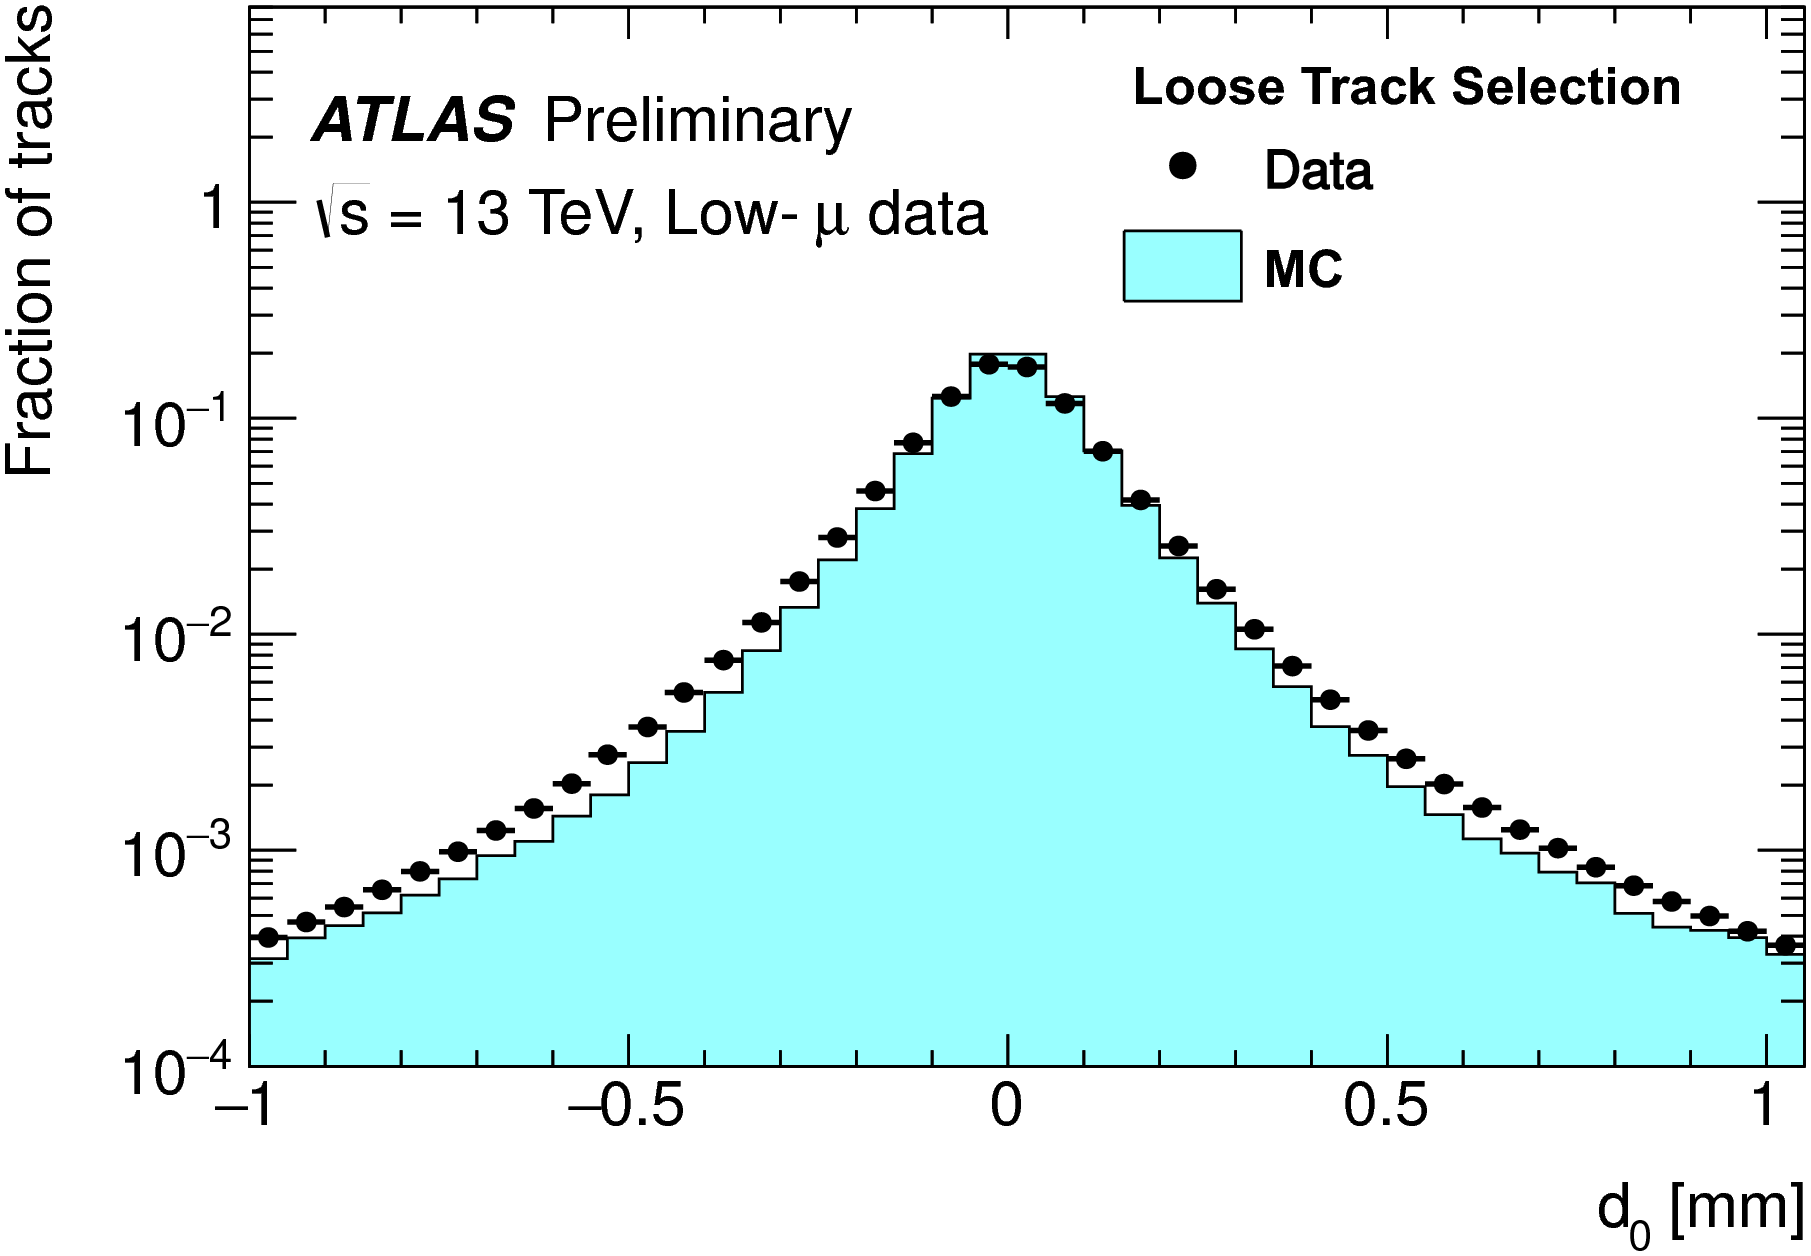
\includegraphics[width=.5\textwidth]{figures/EventReconstruction/ST-d0-eff.png}
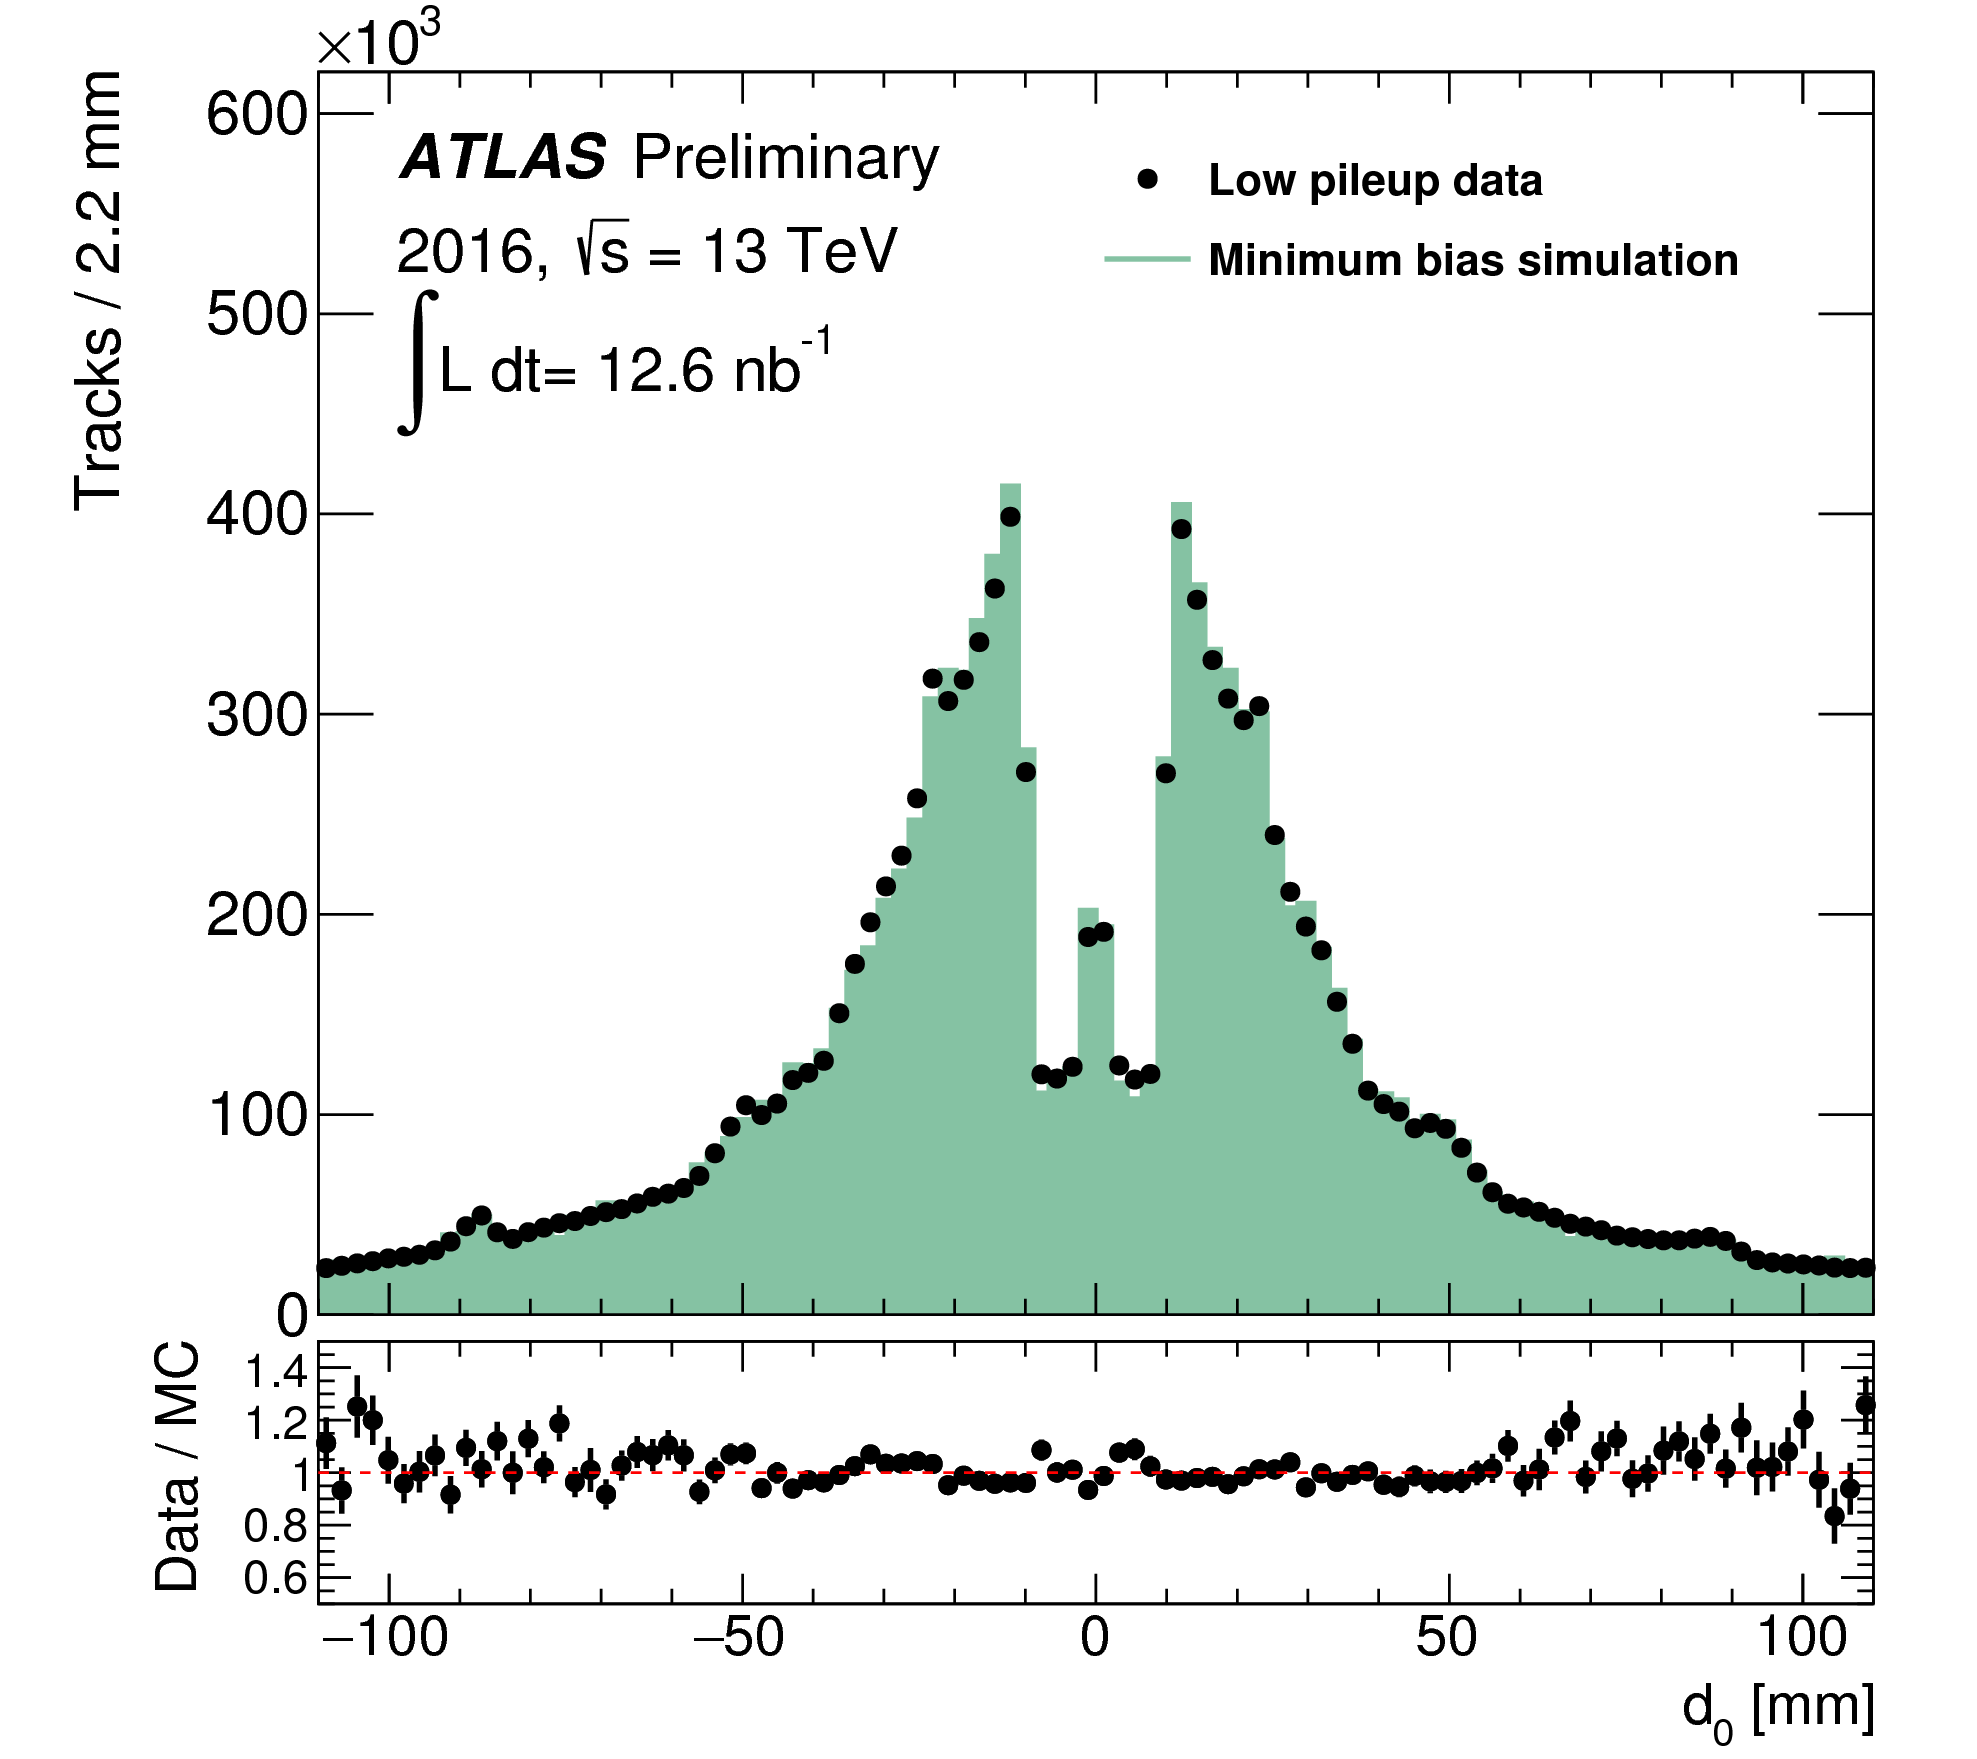
\includegraphics[width=.41\textwidth]{figures/EventReconstruction/LRT-d0-eff.png}
\caption{Number of tracks reconstructed with respect to \dzero in \ac{ST} (left) and \ac{LRT}. Note the difference in x-axis range.}
\label{fig:trking_d0_eff}
\end{figure}

\begin{figure}[htbp]
\centering
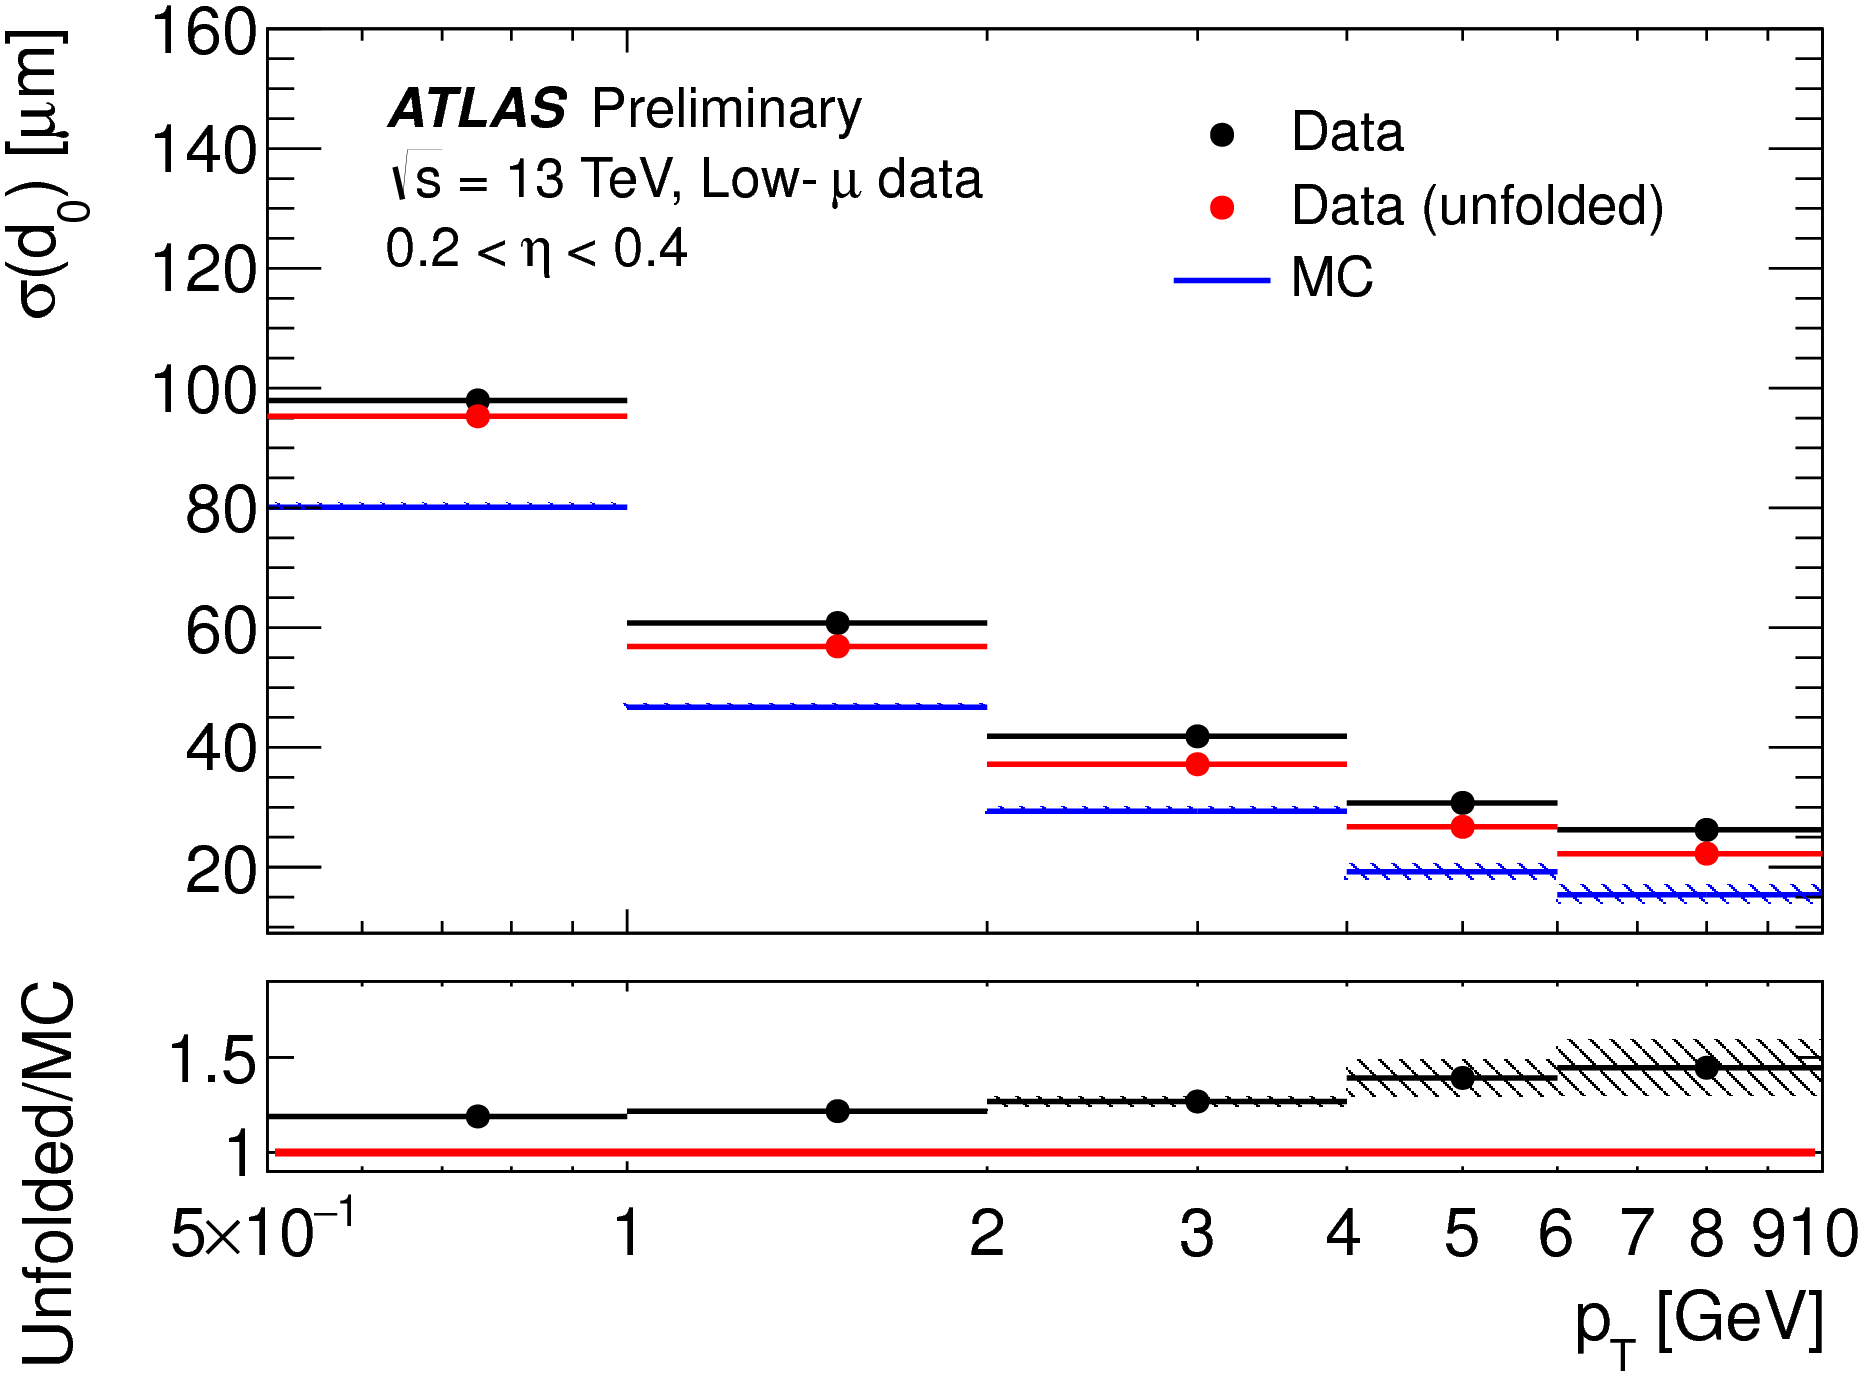
\includegraphics[width=.45\textwidth]{figures/EventReconstruction/ST-d0-res.png}
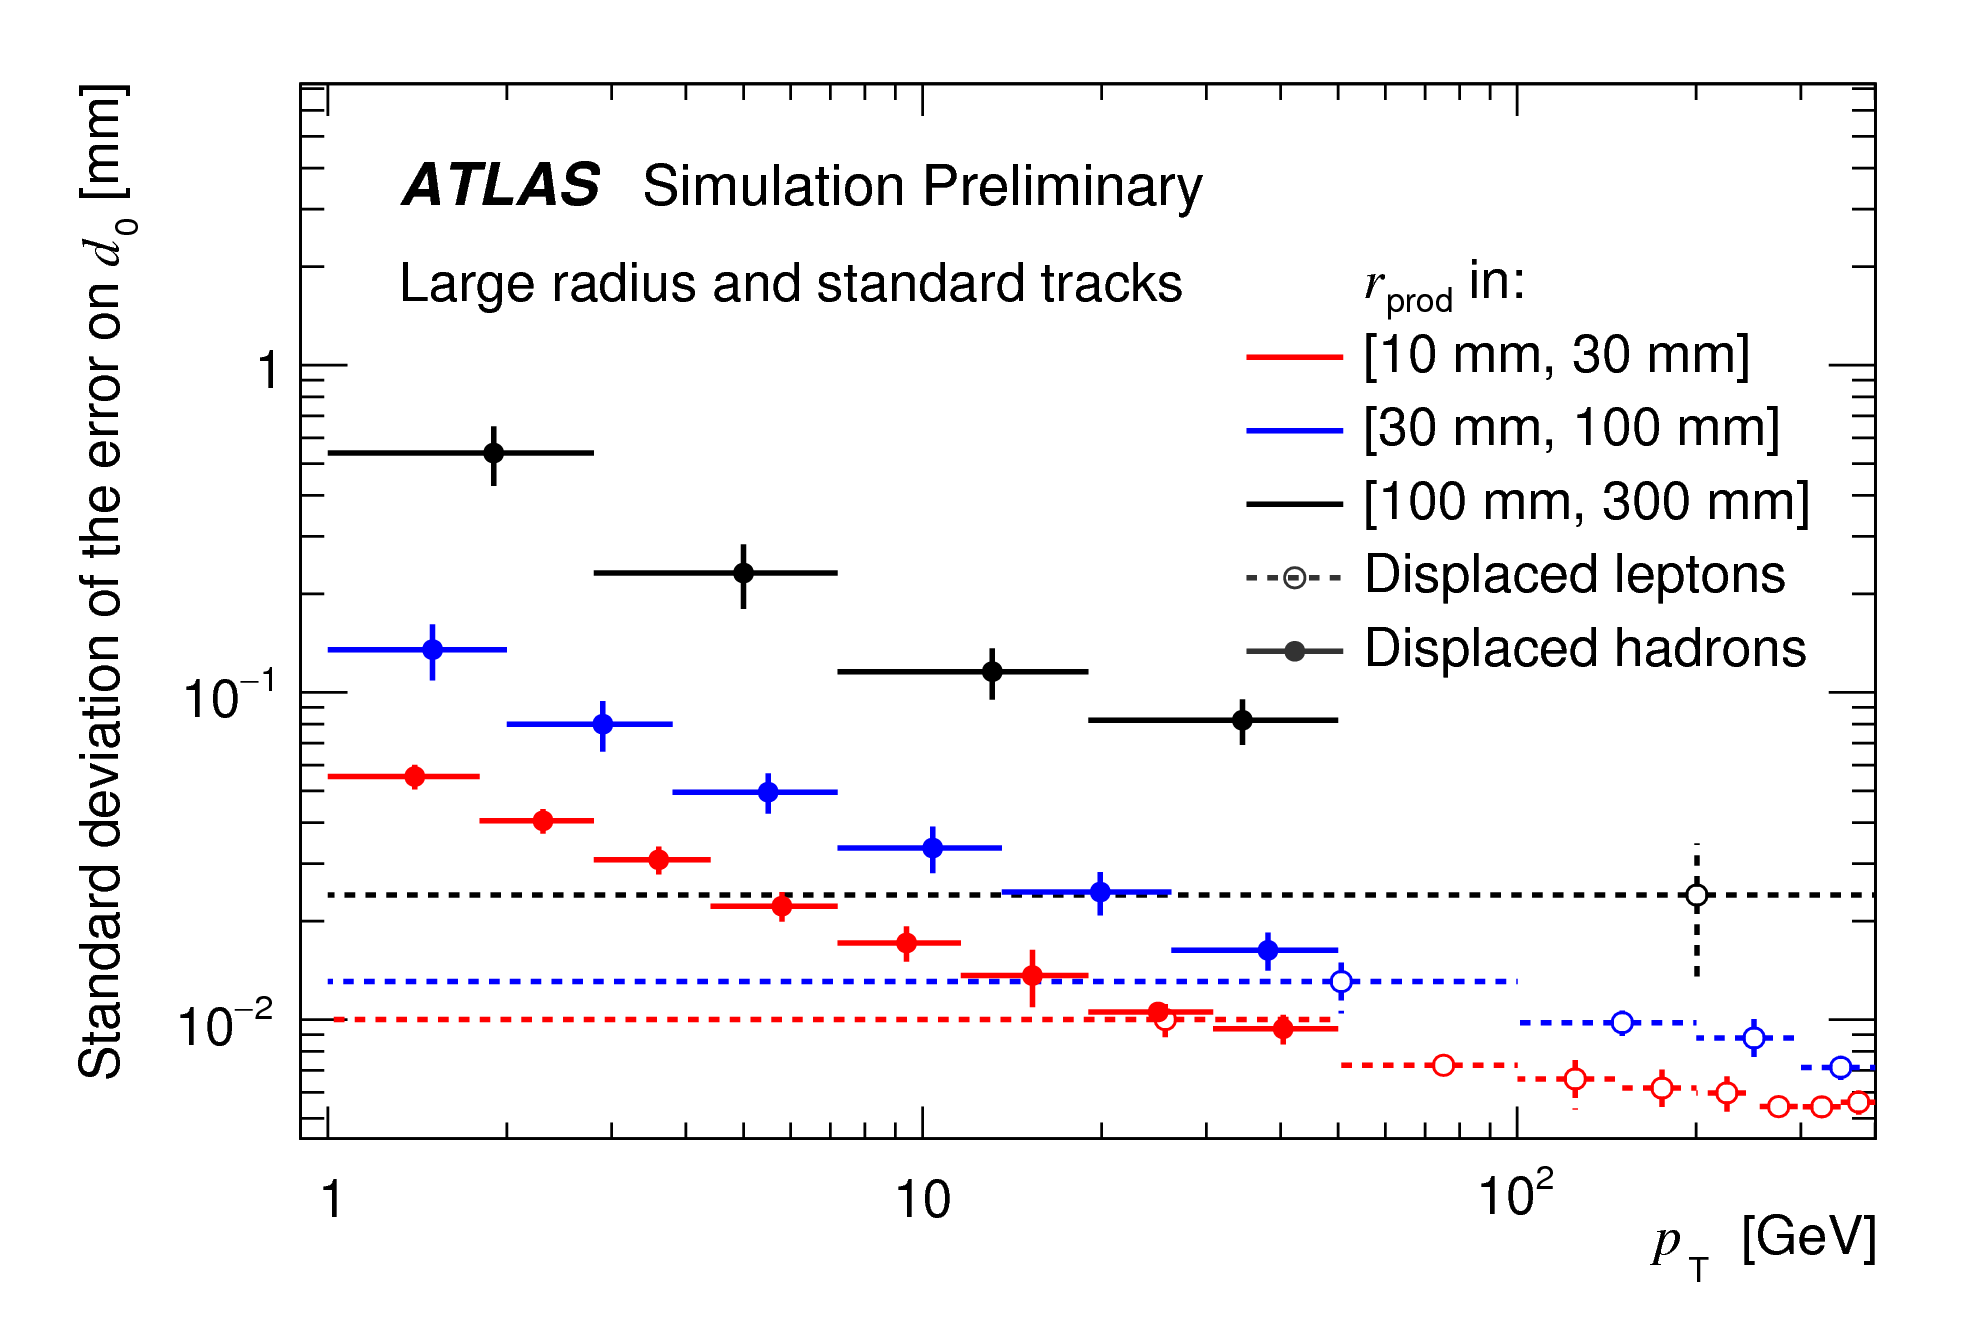
\includegraphics[width=.5\textwidth]{figures/EventReconstruction/LRT-d0-res.png}
\caption{\dzero resolution as a function of \pt in \ac{ST} (left) and \ac{LRT}. This analysis uses high \pt leptons with high \pt tracks, and thus with very good \dzero resolution}
\label{fig:trking_d0_res}
\end{figure}

%mostly used this: https://pdfs.semanticscholar.org/a591/7c383e4b07d64116b57c9c33e82138a08d12.pdf (p19+)
\subsection{Tracking Algorithms}

\subsubsection{\label{sec:kalman} Kalman Filter}

Kalman filters are widely used across LHC experiments for track fitting. It is a recursive algorithm that allows the user to efficiently extrapolate from a track seed. In the sequential, or extended, Kalman filter, uses a linear approximation to the track path. It makes a prediction for the next layer of detector material based on the seed, and then looks for a hit in that region. At each step, it updates the linearization to improve the measurement for the next step, where each measurement is weighted by its certainty. \ac{LRT} uses this approach.

In \ac{ST}, a combinatorial Kalman filter is used. This method employs several Kalman filters running in parallel and allows for the assumption that the measurement in the next layer is not necessarily assumed to be part of the track that formed the seed (as is often the case in the dense environment of the \ac{ATLAS} \ac{ID}). At each successive layer in track finding, several branches are extended if several measurements can be found in the same layer. The update of the linearization is done independently for each branch, and branches are created for missing measurements to account for detector inefficiencies. The branch is extended to the next layer if a measurement is found, and the process is repeated. Branches with no measurement for several layers are removed, and at the end, the branch with the best quality is selected. This process allows for parallelization of a complex combinatorial process. \cite{kalman-filter} 

The Kalman filter works well for tracking in environments such as \ac{ATLAS} because even though it is computationally intensive, it generally gives the best precision.

\subsubsection{\label{sec:hough} Hough Transform}

%https://indico.cern.ch/event/602049/contributions/2429704/attachments/1440531/2217489/Piucci_05_04_2017.pdf
%hough-transform.pdf

A Hough transform is a pattern recognition algorithm that is useful for identifying a particular signature that can be described in a known parametric form. It performs well in noisy environments and is tolerant of holes in the signature. In relies on a transformation from physical to parameter space. Each point in physical space maps to a line in parameter space, and the intersection of the parameter space lines gives the values of constants of the parametric form. 

For example, if the pattern being searched for is a line described by $y = mx + b$, a Hough transform maps from $x-y$ space to $m-b$ space. Each point $(x_i, y_i)$ in the original image maps to a line in parameter space. If all $(x_i, y_i)$ are plotted together, the intersections of the lines in parameter space at $(m_i, b_i)$ define lines in physical space with parameters $m_i$ and $b_i$. \cite{hough-transform}

The Hough transform is a \emph{pattern finding} algorithm, not a tracking algorithm. Is not ideal for full \ac{ID} tracking, because its complexity grows exponentially with the number of dimensions and the form of the pattern must be known \emph{a priori}.

\comebackto{How are seeds formed? Hough transform?}


\subsection{Primary Vertex Reconstruction}

After all of the tracks are reconstructed, they must be correctly assigned to a \ac{PV}. A \ac{PV} is the point in space where the $pp$ collision occurred. Generally, there are many \ac{PV}s per event: one is the hard-scatter, high-energy event of interest, and the others are pileup. In the Run 2 dataset, there are an average of 33 \ac{PV}s per event.

\ac{PV}s are reconstructed using an n iterative vertexing procedure. First, good quality tracks tracks, combined with the beamspot measurement, are used to find an optimal vertex position. Then each track is assigned a weight based on its compatibility with that position, and the vertex position is then recomputed using the weights of the tracks. After the final vertex position is determined, tracks very incompatible with the vertex are removed from it and can be used to create another vertex. Any vertex with at least two tracks are considered \ac{PV}s.



%-----------------------------
% Muon Reconstruction
%-----------------------------
\section{Muons}
%USED atlas-muon-reco.pdf
\label{sec:muonreco}
\subsection{Standard Reconstruction and Identification}

Muons are reconstructed by combining a \ac{MS} track with an \ac{ID} track. Then, at the identification stage, quality requirements are imposed on the combined tracks to improve the purity of the muon collection. For this analysis, the muon reconstruction algorithm remains unchanged (though \ac{LRT} tracks are used), while changes are made at the identification stage. \cite{muon-reco}

\subsubsection{Muon Track Reconstruction}
To reconstruct \ac{MS} tracks, a Hough transform (described in \autoref{sec:hough}) is used to search for hits in each \ac{MDT} chamber to find hits following a trajectory on the $\eta$ plane of the detector. These hits are fit to a straight line within each chamber to form \emph{segments}. Co-located \ac{RPC} and \ac{TGC} hits are used to measure the $\phi$ coordinate. 

Hits from segments in various layers are fit to form track candidates. This fitting is first seeded from segments in the middle layers of the \ac{MS} where more trigger hits are available, then extrapolated inward and outward. A next pass is done using inner and outer station segments as seeds. The extrapolation relies on relative positional and angular information, as well as the fit quality and hit multiplicity of the segments. Two segments are required to make a track, except in regions with limited detector coverage, where one high quality segment is sufficient. After all extrapolation, an overlap removal procedure is performed, allowing for a segment to be shared between at most two tracks. A $\chi^{2}$ test is performed, where outliers hits can be removed from the track and additional hits consistent with the track candidate's trajectory can be added.

\comebackto{what are "trigger hits"}


\subsubsection{Combined Muons}
Next, the \ac{MS} tracks are combined with \ac{ID} tracks to form \ac{CB} muons, a track fit over the two tracks. \ac{CB} muon tracks are generally seeded from the \ac{MS}, then extrapolated inward and matched to an \ac{ID} track, but the inverse is also allowed. Hits from the \ac{MS} may be added or removed to improve the fit between the two tracks.



\subsubsection{Muon Identification}

This analysis uses the default muon working point for ATLAS analyses, called a \emph{medium} muon. This working point places a requirement on the number of \ac{ID} and \ac{MS} hits that comprise the track to ensure a robust momentum measurement. At least 1 pixel hit, at least 5 \ac{SCT} hits are required and at least 10\% of the \ac{TRT} hits associated to the object must be included in the final fit. There must also be fewer than 3 holes in the silicon tracking layers. Furthermore, the \ac{MS} track must have at least 3 hits in at least 2 \ac{MDT} layers. In the crack region $|\eta| < 0.1$, \ac{MS} tracks with at least three hits in only one \ac{MDT} layer are allowed provided there are no holes in the track. Finally, a loose requirement is placed on the consistency between the \ac{MS} and \ac{ID} tracks. Namely, the \emph{q/p significance}, the difference between the charge and momentum ratio in the \ac{ID} and \ac{MS} divided by their uncertainties summed in quadrature, is required to be less than 7. 


\begin{figure}[htbp]
\centering
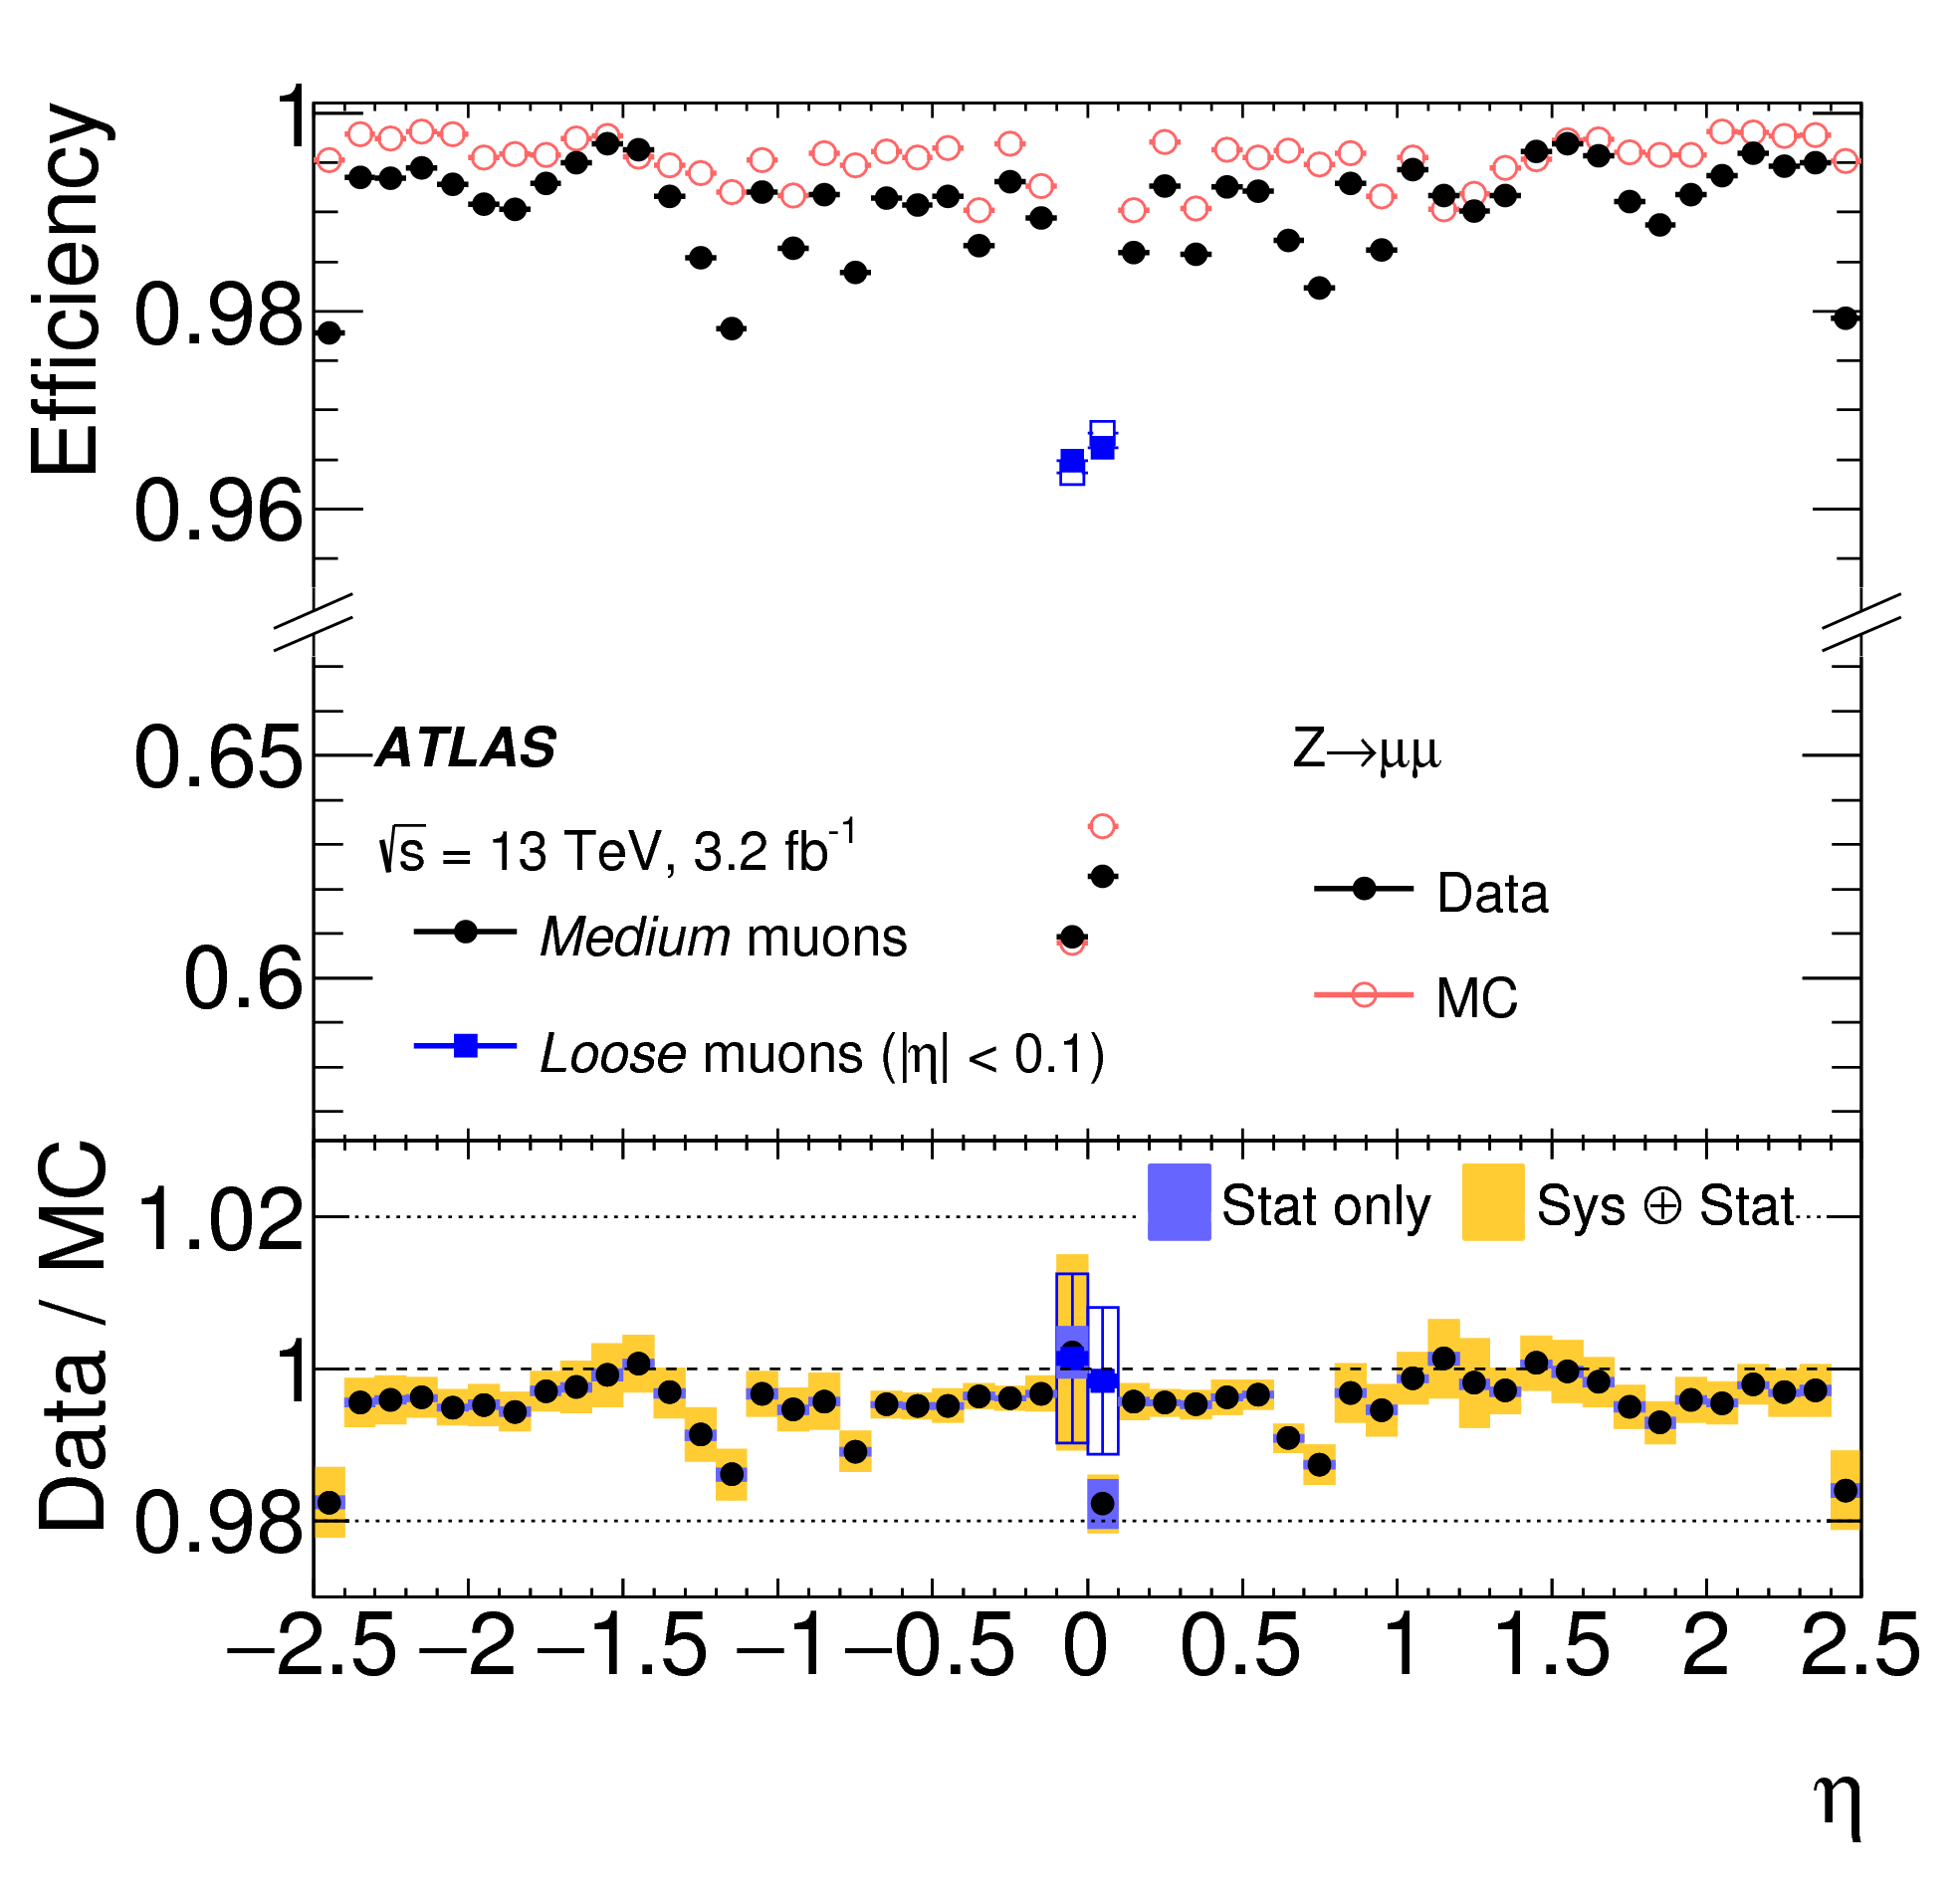
\includegraphics[width=.43\textwidth]{figures/EventReconstruction/muon-reco-eta.png}
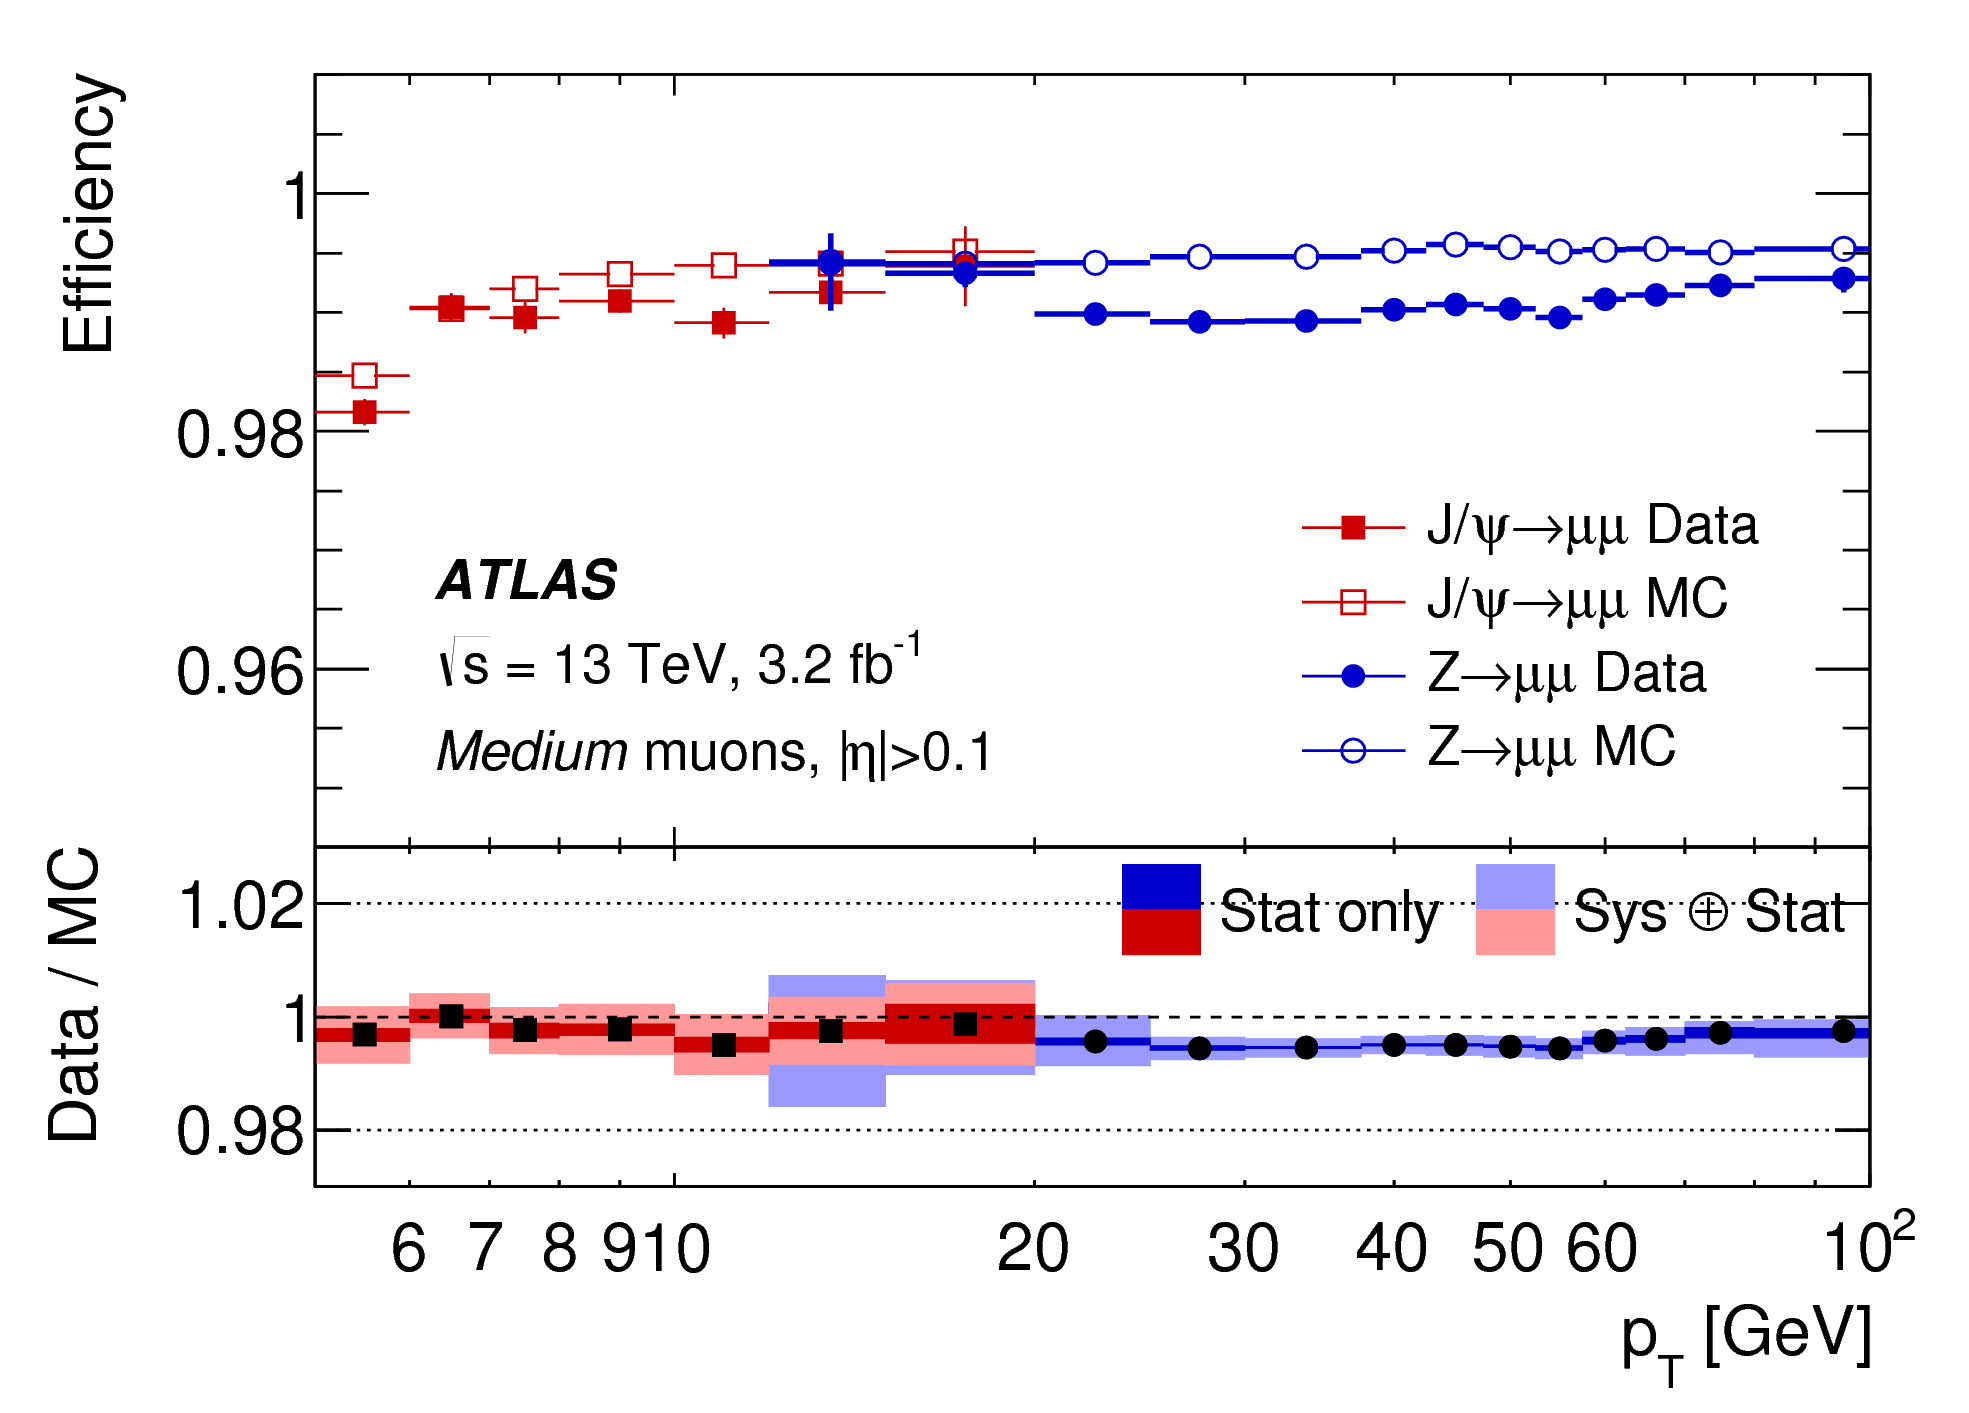
\includegraphics[width=.52\textwidth]{figures/EventReconstruction/muon-reco-pt.png}
\caption{Medium muon identification efficiency with standard tracking and criteria. Left is efficiency vs $\eta$ and right is efficiency as a function of $p_{T}$. Medium muons are reconstructed very efficiently, except for around $|\eta| \approx 0$, where the \ac{MS} is missing detector coverage.}
\label{fig:std_muon_eff}
\end{figure}


\subsection{Modifications}
\label{sec:mu_reco_mods}

For this analysis, muons are reconstructed after \ac{LRT} is performed and the reconstruction and identification efficiency is quite high. Furthermore, at the identification stage, we remove the requirement that the \ac{ID} track has at least one pixel hit, further improving the efficiency at high $d_{0}$. The effect of these improvements is show in \autoref{fig:cust_muon_eff}


This modification of the muon identification increases the fake rate of muons, so again we impose quality requirements that are independent of displacement. We require the muon to have at least two \ac{MS} layers with at least three precision hits, that the muon have at least one $\phi$ measurement (otherwise the \ac{MS} $\phi$ measurement is taken as the center of the \ac{MDT}, with an uncertainty of 0.2) and require the $\chi^{2}_{CB}/N_{DoF} < 3$. The $\chi^{2}_{CB}$ requirement is, in effect, a requirement on the consistency between the the \ac{ID} and \ac{MS} tracks. These will be further discussed in \autoref{sec:mu_qual_req}


\begin{figure}[htbp]
\centering
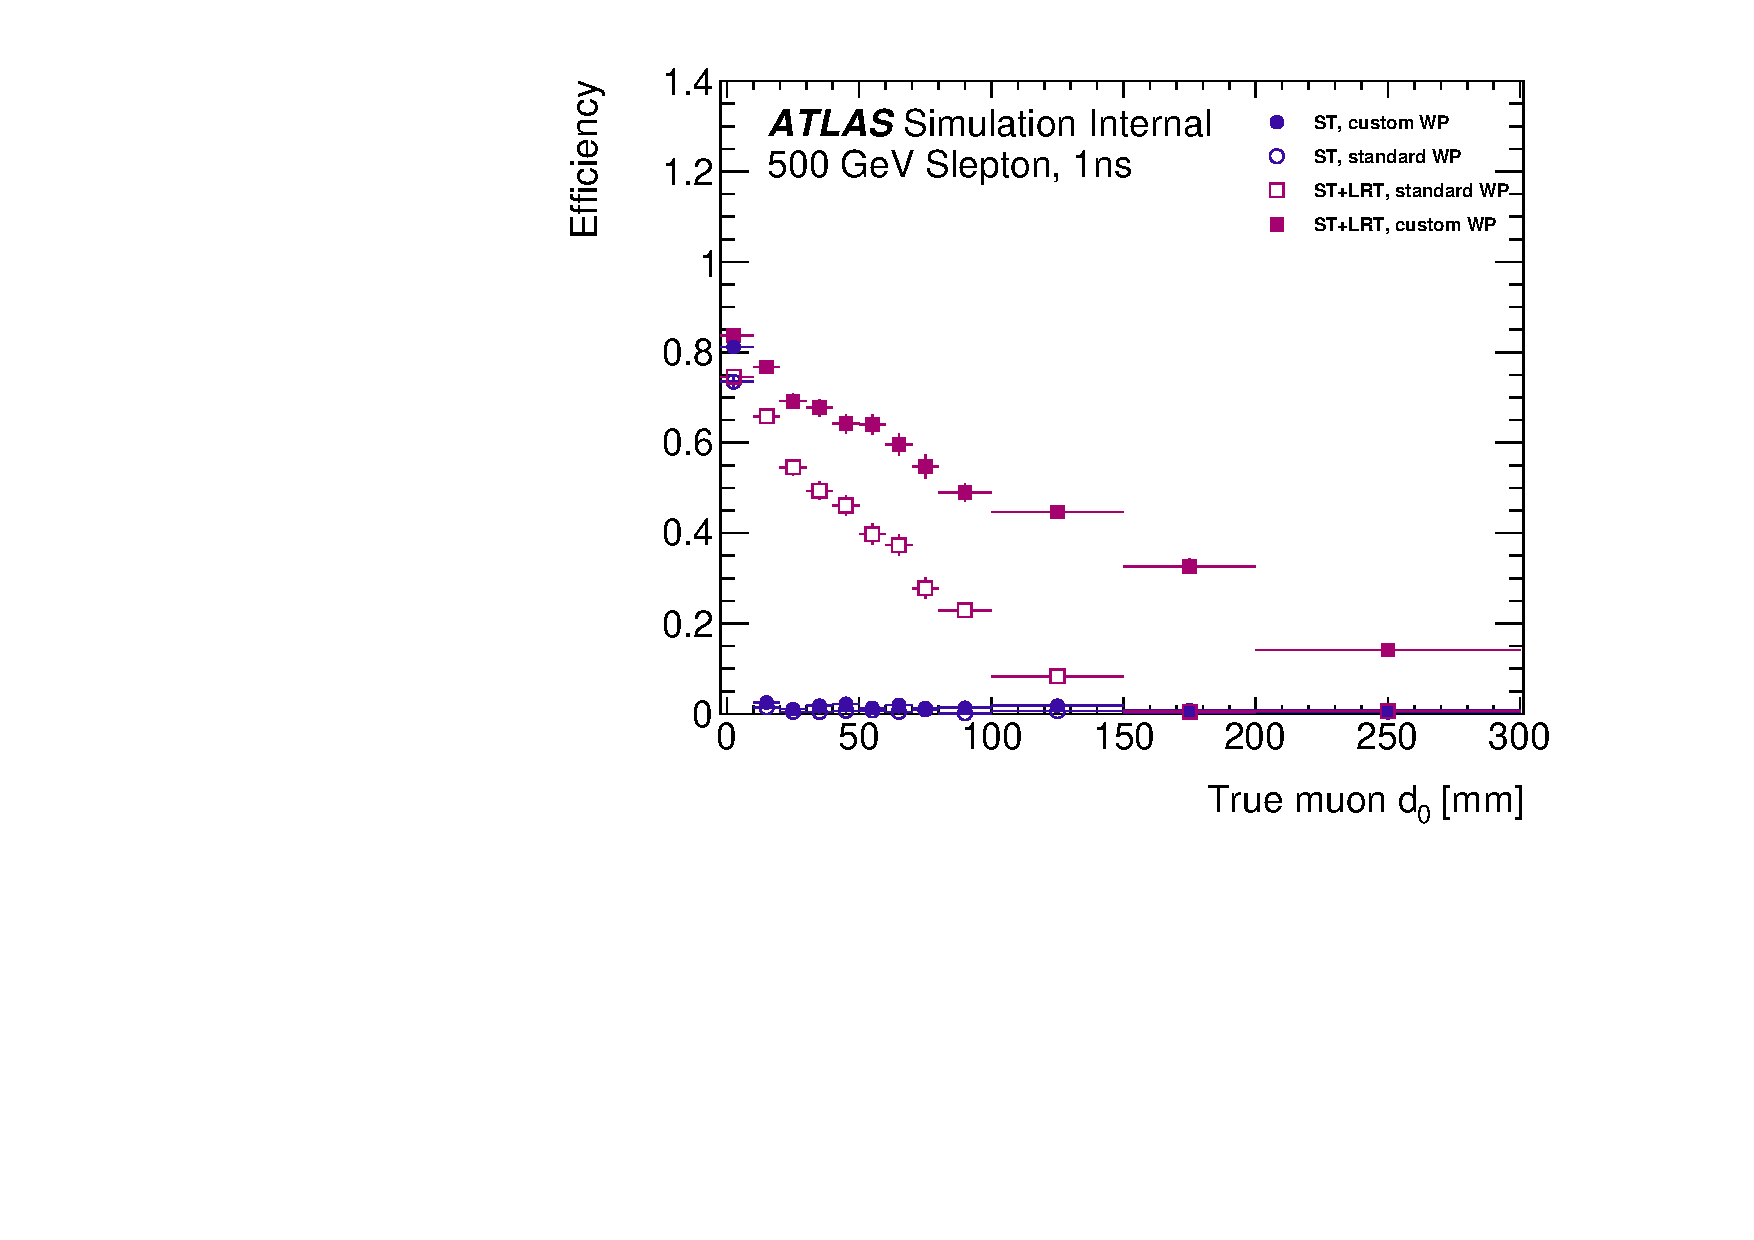
\includegraphics[width=.48\textwidth]{figures/EventReconstruction/wp_m_d0_all_wip.pdf}
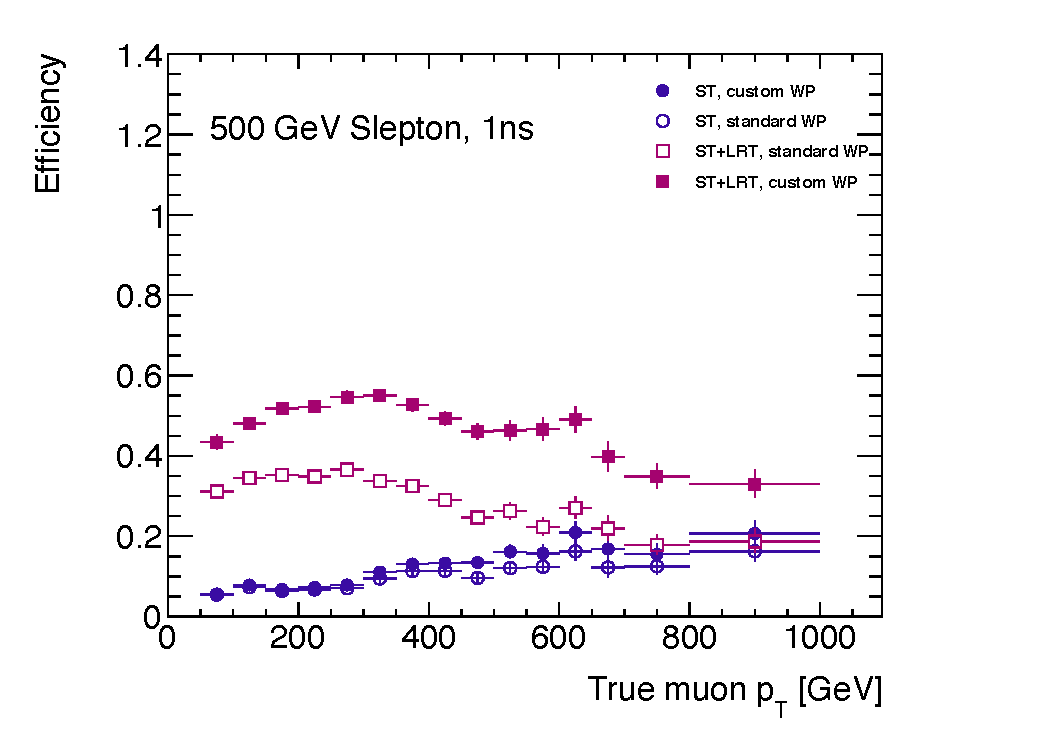
\includegraphics[width=.48\textwidth]{figures/EventReconstruction/wp_m_pt_all_wip.pdf}
\caption{Muon identification efficiency with modified criteria. Left is efficiency vs $d_{0}$ and right is efficiency as a function of $p_{T}$. The red denotes reconstruction with Standard Tracking (ST), and the blue with Large Radius Tracking (LRT), and the filled in circles use the modified identification working point. \todo{Needs update when available}}
\label{fig:cust_muon_eff}
\end{figure}



%-----------------------------
% Electron Reconstruction
%-----------------------------
\section{Electrons}
%USED atlas-electron-reco.pdf atlas-electron-reco-sliding-window.pdf
\label{sec:elecreco}

Electrons are reconstructed using clusters from the \ac{EM} calorimeter as well as tracks from the \ac{ID}. \cite{electron-reco} Electron reconstruction brings more complication and ambiguity than muon reconstruction because of the presence of photons, converted photons, and bremsstrahlung radiation from electrons moving through material. These factors make the identification and accurate measurement of electrons quite challenging. More than in muon reconstruction, it relies on displacement-based quality information, posing a problem for this search. We modify these requirements and use \ac{LRT} tracks, but have a resulting lower selection efficiency. 

\subsection{Standard Reconstruction and Identification}


\subsubsection{Cluster Reconstruction}

First, clusters are formed from $\eta \times \phi$ \emph{towers} of size $\Delta \eta \times \Delta \phi = 0.025 \times 0.025$ (roughly granularity of the second layer of the \ac{EM} calorimeter, where about 80\% of the energy in a shower is deposited). In each region, the energy deposited in all layers of the calorimeter is summed and are used as input to a seeding algorithm to form clusters. 

A \emph{sliding window} algorithm \cite{electron-sliding-window} is used to form clusters. In this algorithm, an $3 \times 5$ window is slid across each tower, the energy is summed inside of this window. If the sum is a local maximum and is above a threshold of $\et > 2.5 \GeV$, this window is considered a \emph{cluster}. A duplicate removal process is then performed for nearby clusters with similar energy measurements, keeping only the cluster with the largest $E_{T}$. Inefficiency in the cluster reconstruction step is negligible compared to the uncertainty in the next two steps. The efficiency of this step is 65\% at $\et = 4.5 \GeV$ and $> 99\%$ above $\et = 15 \GeV$.

\begin{figure}[htbp]
\centering
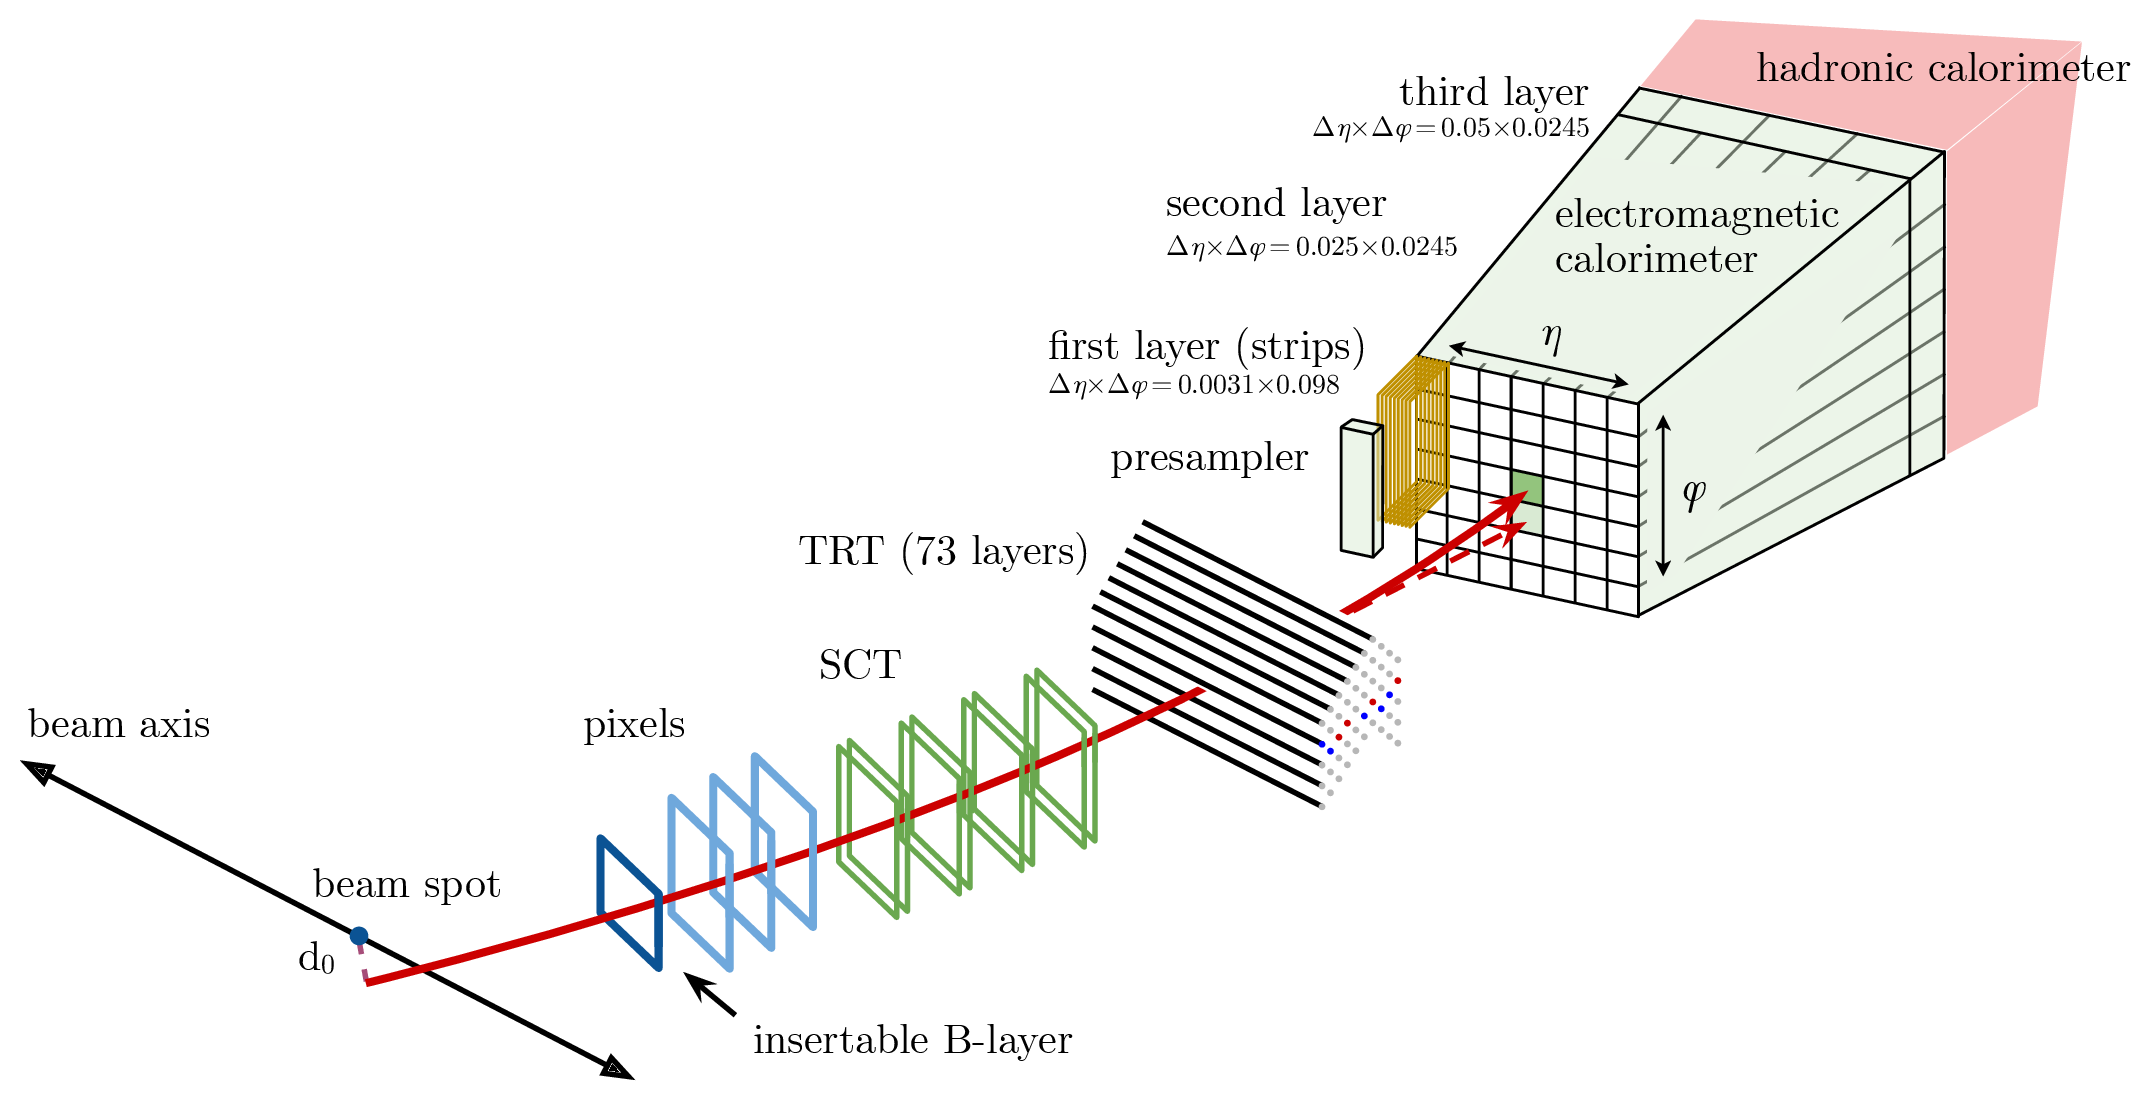
\includegraphics[width=.8\textwidth]{figures/EventReconstruction/electron-reco-sketch.png}
\caption{A sketch of an electron's path through a slice of the \ac{ATLAS} detector.}
\label{fig:elec_reco_sketch}
\end{figure}

\subsubsection{Tracking}
Since electrons are so light, they can lose a significant amount of their energy due to bremsstrahlung radiation as they traverse the \ac{ID}, thus resulting in a track seed that cannot be extended to the requisite number of silicon layers using the processes described in \autoref{sec:trackreco}. Thus, a second pass at tracking, allowing for 30\% energy loss due to bremsstrahlung radiation at each detector layer is performed in the vicinity of a good quality \ac{EM} cluster. Here, the track candidate $p_{T}$ is lowered to $400 \MeV$ (compare to $1 \GeV$), but still uses the standard hypothesis that the track is like that from a pion. If this fit still fails, a third pass is performed using the assumption that the track is like that from an electron, allowing for an additional degree of freedom in the $\chi^2$ calculation that accounts for additional radiation. In all, this gives 98\% reconstruction efficiency for electrons with $\et > 10 \GeV$. 

This loosened track fitting requirements allow for increased efficiency, but the resulting tracks do not correctly account for the energy loss of the electron to the material. An additional tracking pass, using an optimized \ac{GSF} is used to correct for this. 

This procedure is performed on tracks with at least 5 silicon hits and roughly match to an \ac{EM} cluster. The \ac{GSF} procedure is based on a combinatorial Kalman filter, resulting in track parameters weighted by Gaussian function describing material-induced energy losses. This procedure also accounts for the increase in curvature caused by the decrease in momentum due to energy loss in material, improving the calculation of track parameters. An example of this is show in the figure below. The reconstruction efficiency for this step is around 98\% for electrons with $\et > 30 \GeV$. 

\begin{figure}[htbp]
\centering
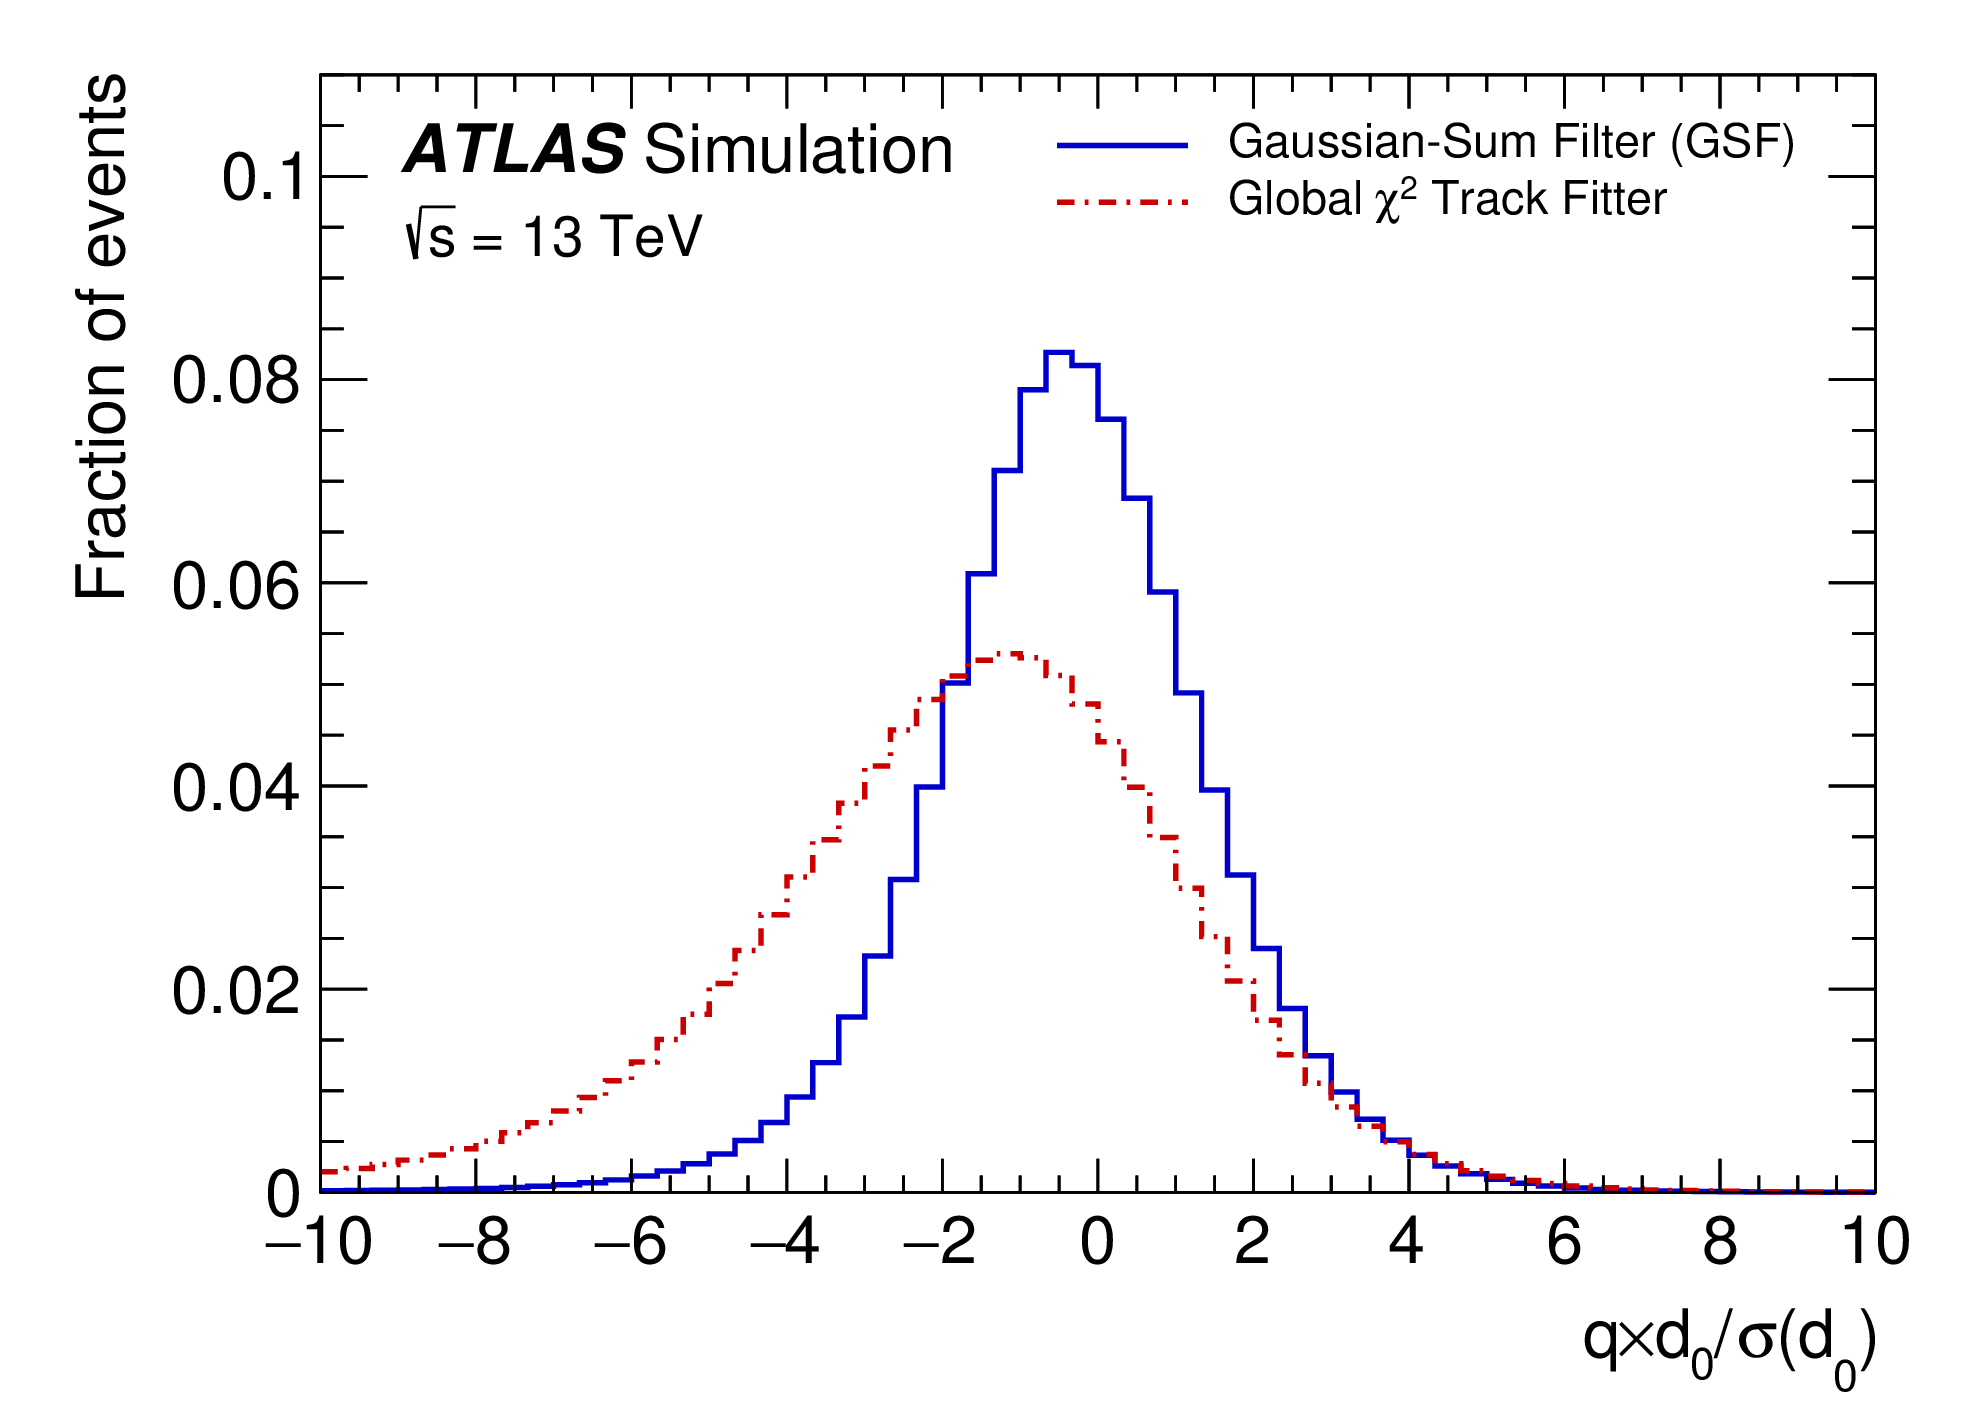
\includegraphics[width=.7\textwidth]{figures/EventReconstruction/elec-qxd0.png}
\caption{The impact on the $q \times \dzero /\sigma(\dzero)$ measurement by the addition of \ac{GSF} tracking. This is sampled from prompt electrons, so the narrower distribution centered around zero indicates significant improvement.}
\label{fig:elec_gsf}
\end{figure}


\subsubsection{Combined Reconstruction}
To put it all together, \ac{GSF} tracks are then matched to seed calorimeter clusters then the final cluster size is determined. Tracks and clusters are matched with stricter requirements, requiring that their $\phi$ measurement is within $+0.05$ or $-0.10$. It is possible that several tracks might match to the same cluster, but a primary track is assigned based on its proximity and quality. If the track can be associated to a vertex, it is classified as a potential photon conversion, not an electron. Electrons are further distinguished from photon conversions using their $E/p, p_{T}$, and number of pixel hits. 

Final clusters are formed by looking in a window around the seed cluster. The reconstructed electron's energy measurement is taken from its full cluster, and directional information taken from its track. At $\et > 15 \GeV$, there is a 99\% efficiency to reconstruct an electron (provided it has at least one pixel hit and at least seven total silicon hits on track). 

\begin{figure}[htbp]
\centering
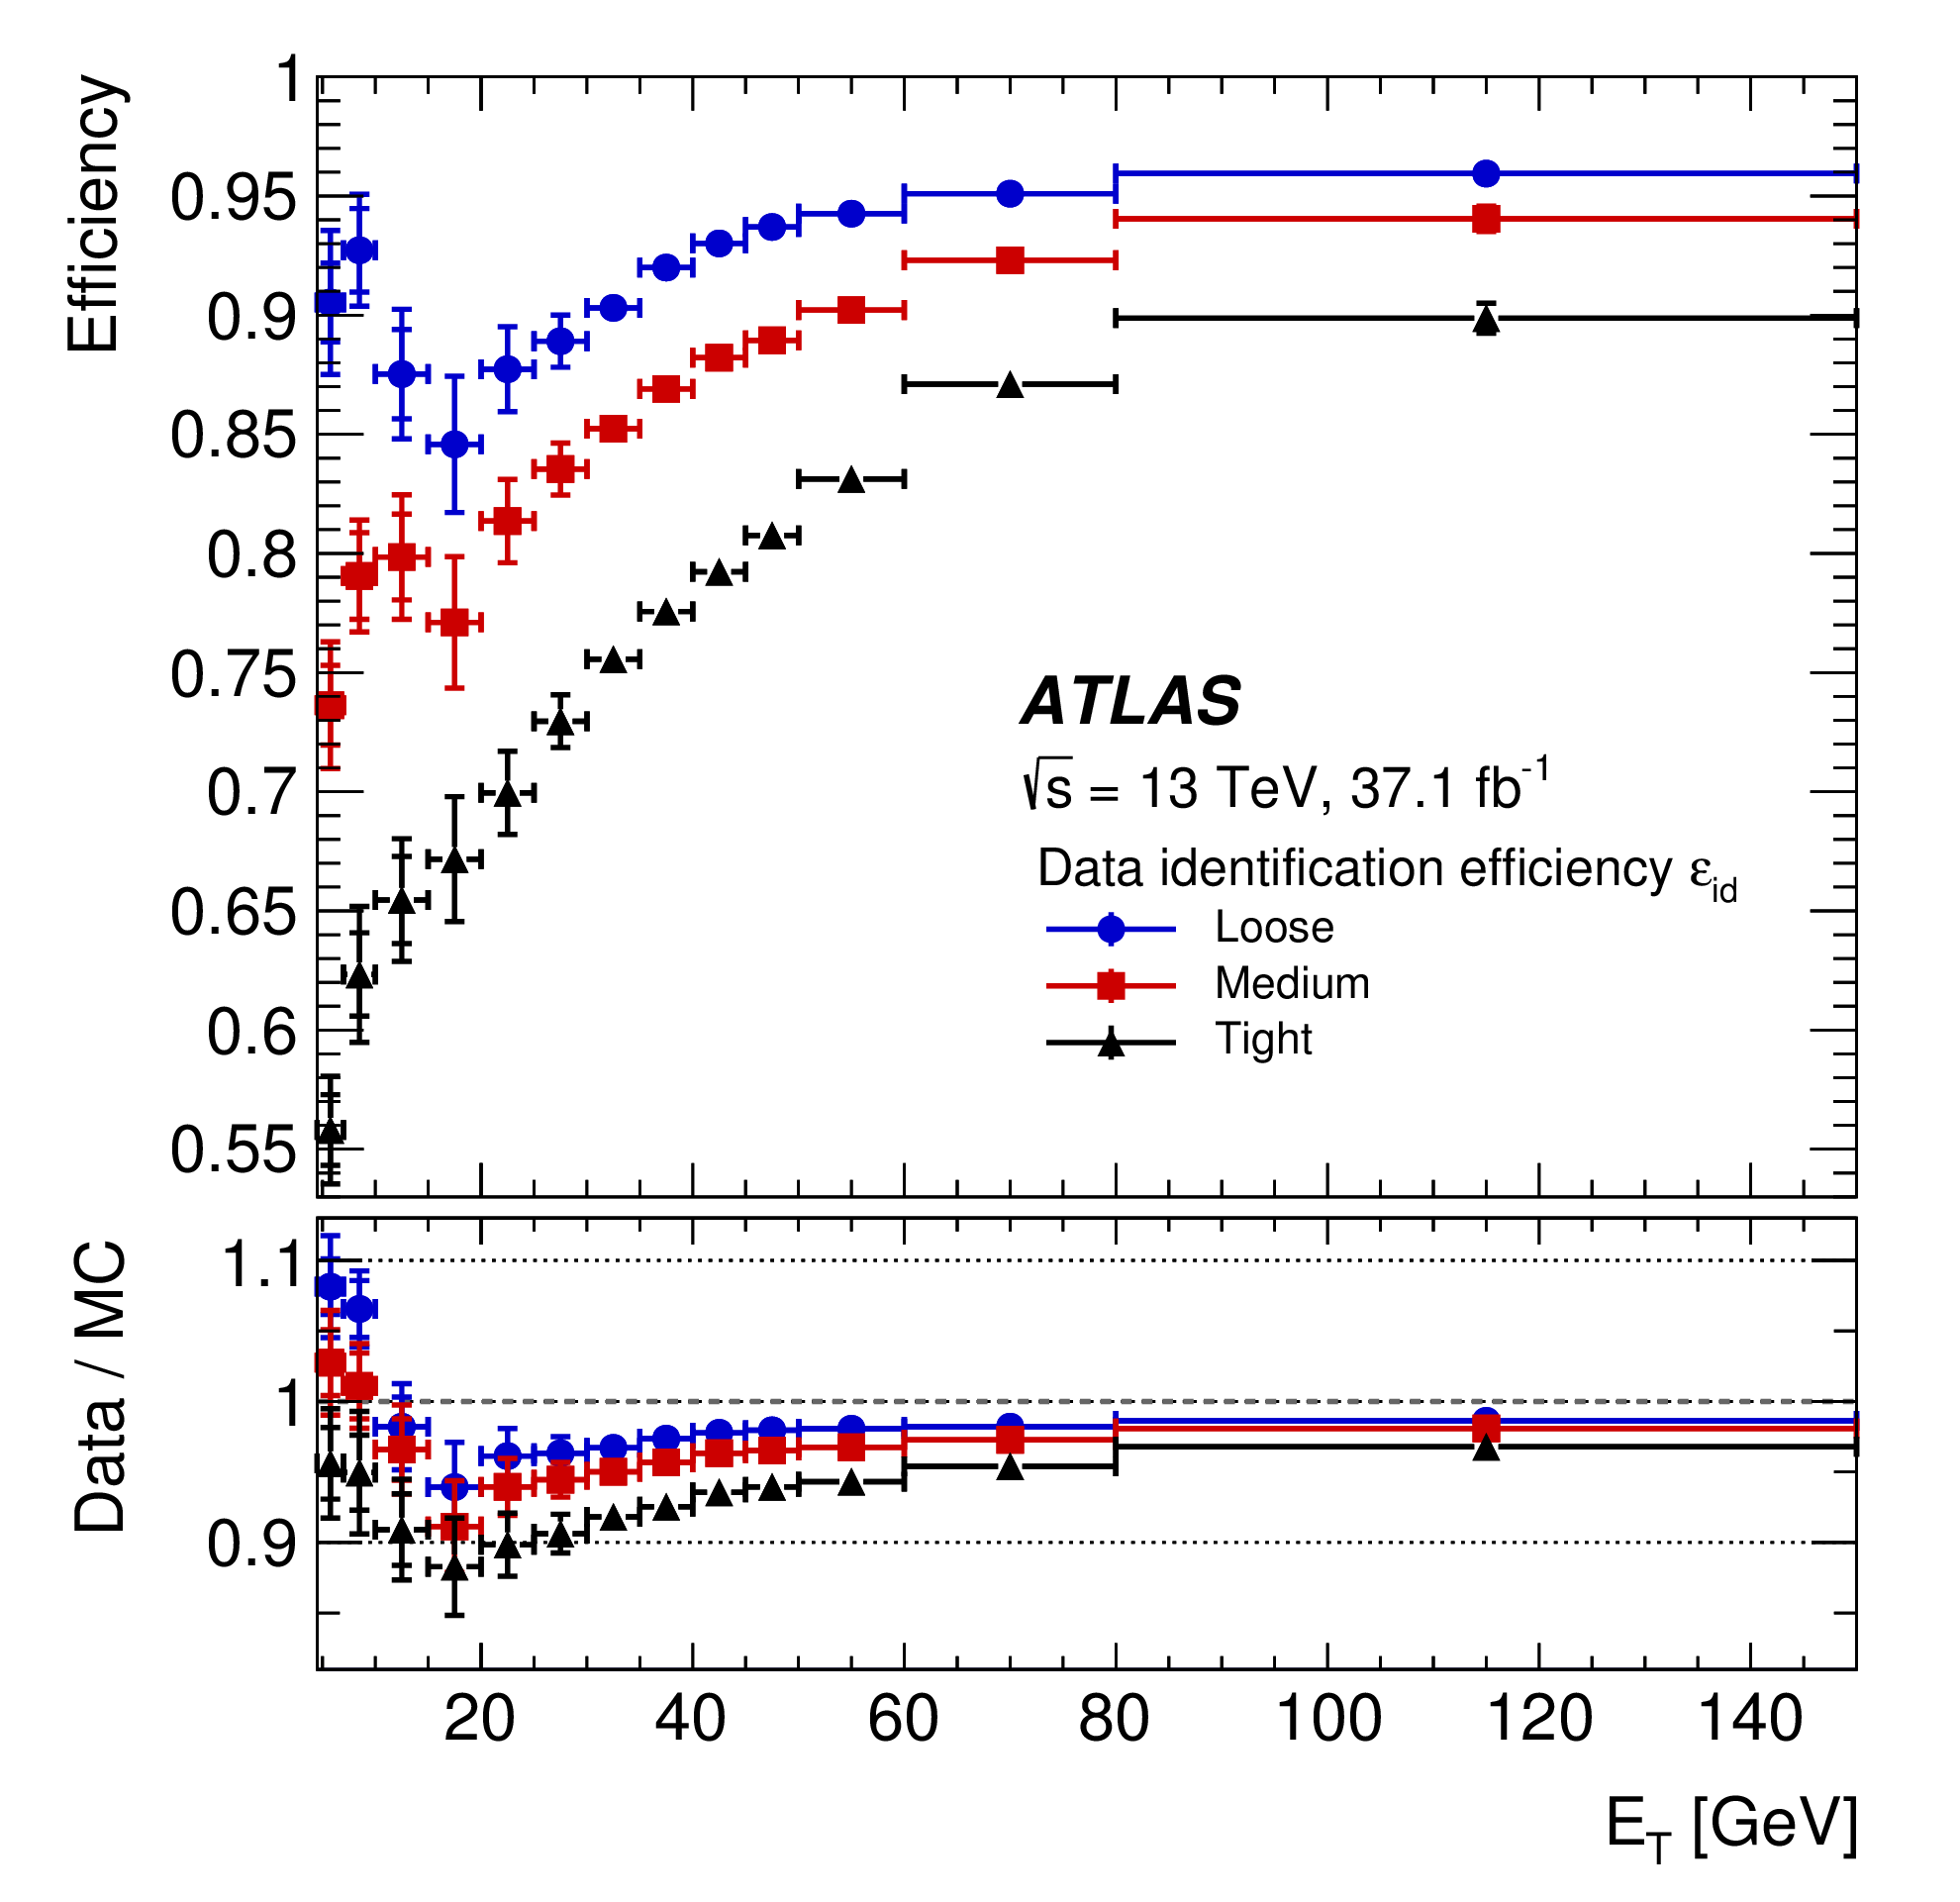
\includegraphics[width=.4\textwidth]{figures/EventReconstruction/elec-reco.png}
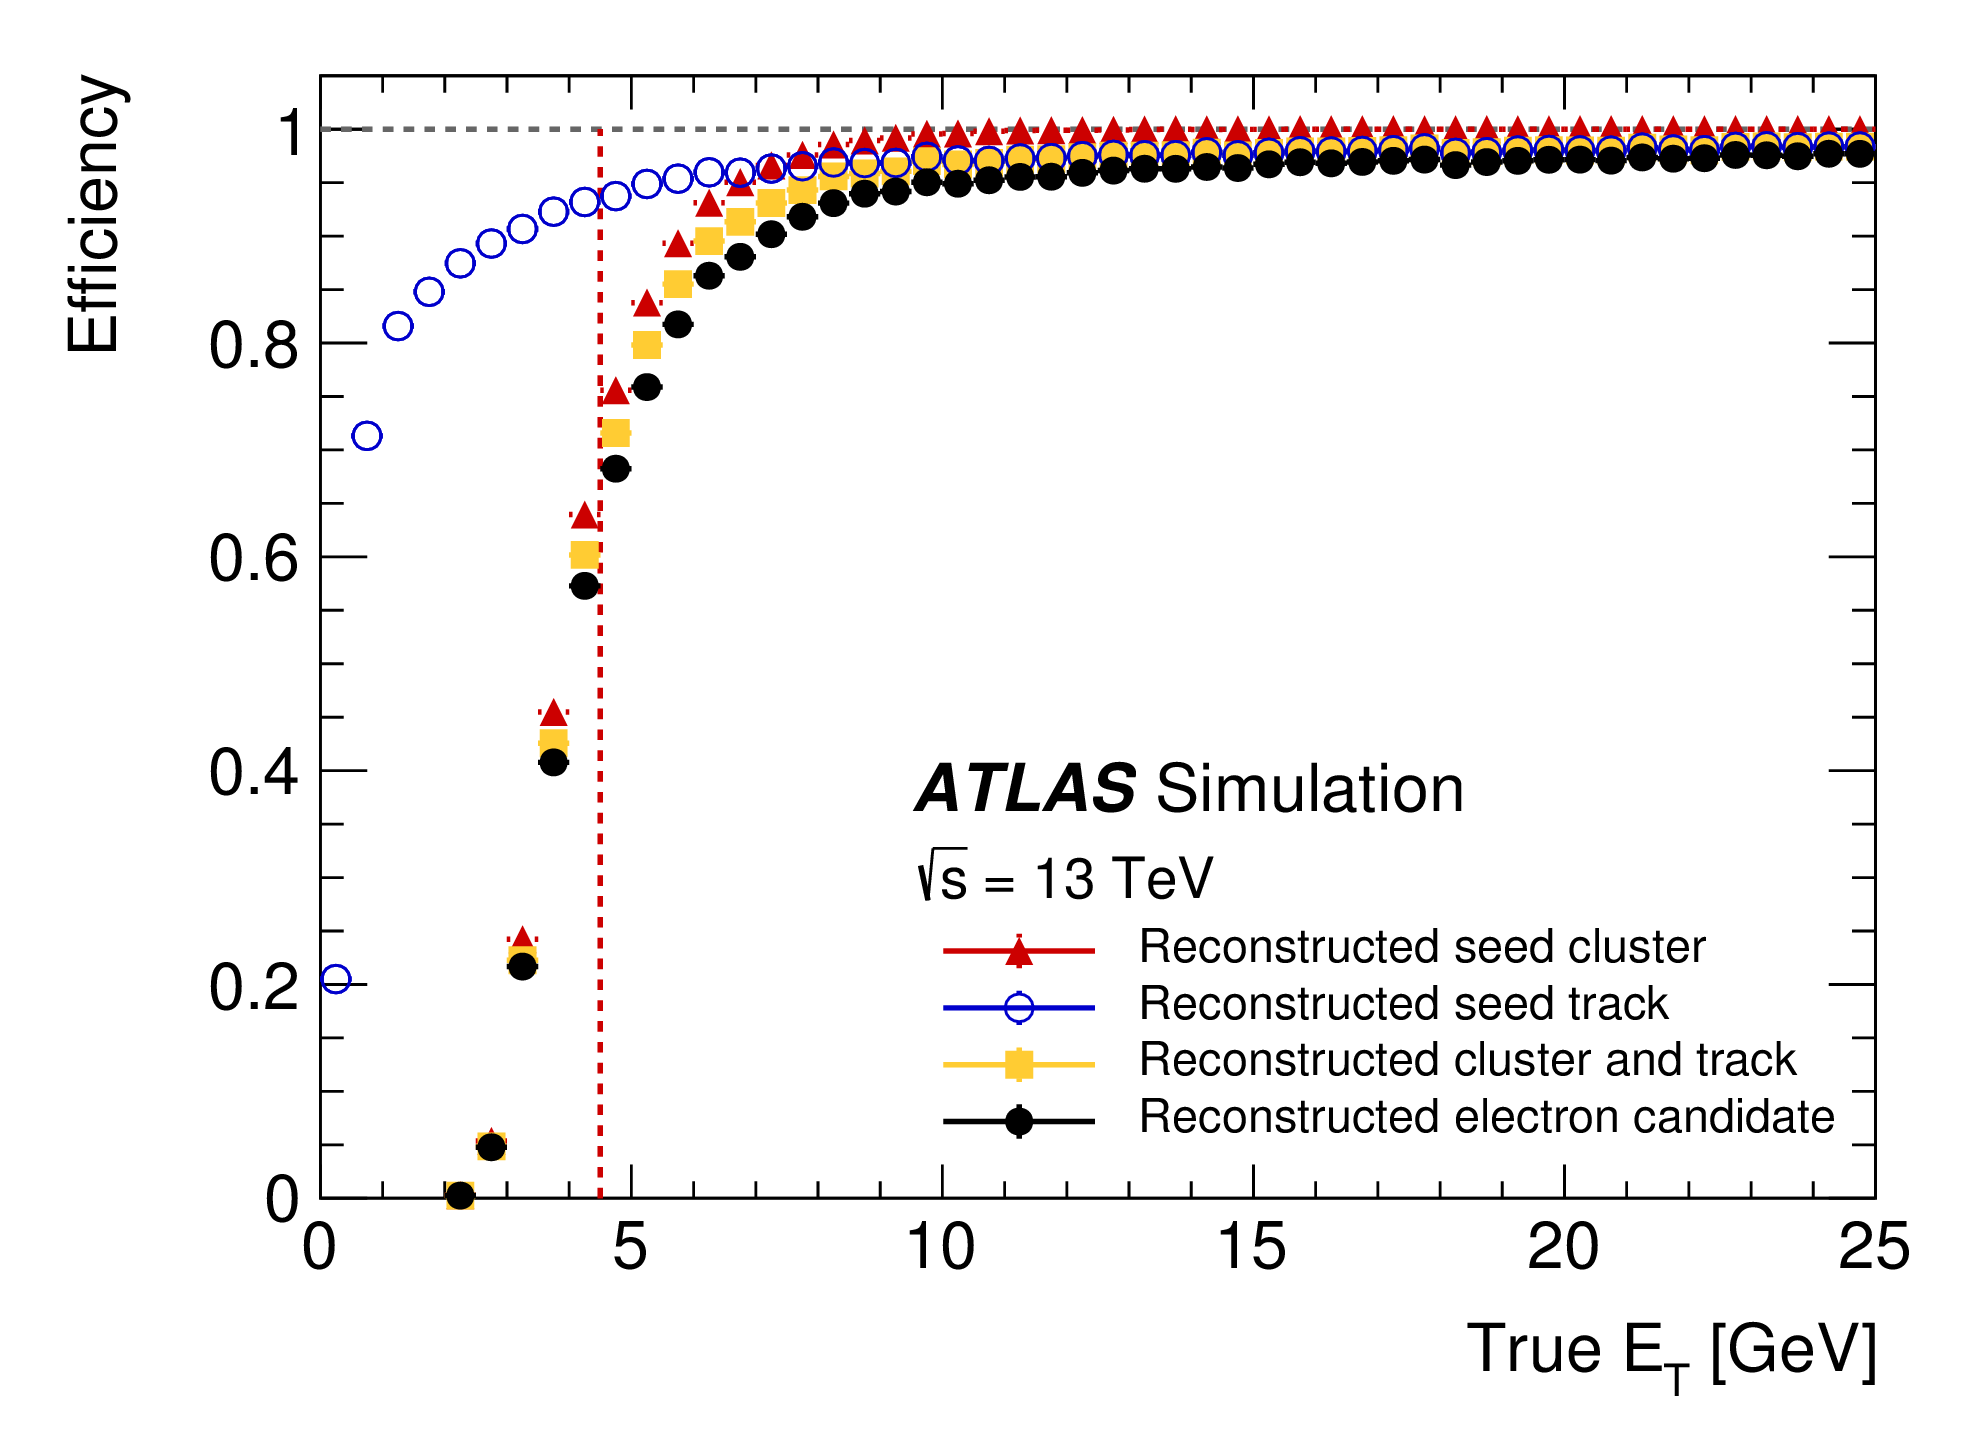
\includegraphics[width=.5\textwidth]{figures/EventReconstruction/elec-reco-steps.png}
\caption{Electron reconstruction efficiency as a function of true transverse energy, \et. For the various electron working points (left) and for each step in the reconstruction process (right).}
\label{fig:elec_gsf}
\end{figure}

\subsubsection{Identification}

Electrons are identified using a likelihood that further distinguishes them from photons, light flavor jets, and leptonic heavy flavor decays. The likelihood is more flexible than a simple cut-based method, allowing for electrons to fail one selection criterion. It also allows for the use of discriminating criteria which have relatively similar shapes in signal and background. A some cuts are made at the identification step, including on the number of pixel and silicon hits, as well as on the shower width. Many other factors not cut on but are included in the likelihood including the track quality, consistency between the electron's track and its cluster, as well energy ratios in the various layers of the \ac{EM} calorimeter, as well as the \ac{EM} calorimeter compared to the hadronic calorimeter.


\subsection{Modifications}
\label{sec:el_reco_mods}
To be able to reconstruct electrons with high impact parameter, several changes needed to be made to the reconstruction and identification algorithms. 

Similar to the muon case, the reconstruction is then run on the track collection including \ac{LRT} tracks. At the identification stage, we remove variables concerned with $d_{0}$ from the likelihood consideration, but do not retrain the likelihood itself. We also remove the cut on the number of silicon hits on top of that made at the reconstruction stage. 

After these modifications, we introduce many fake electrons, primarily resulting from a fake \ac{LRT} track being associated to an \ac{EM} cluster from a photon. The most powerful discriminator is the consistency in the $p_{T}$ as measured by the track and the cluster, defined as $\Delta p_{T} = p_{T}^{track}/p_{T}^{e}$. Furthermore, we require the primary track to be good quality, with $\chi^{2} < 2$ and at maximum one missing hit on track after the innermost hit. These will be further discussed in \autoref{sec:elec_qual_req}

\begin{figure}[htbp]
\centering
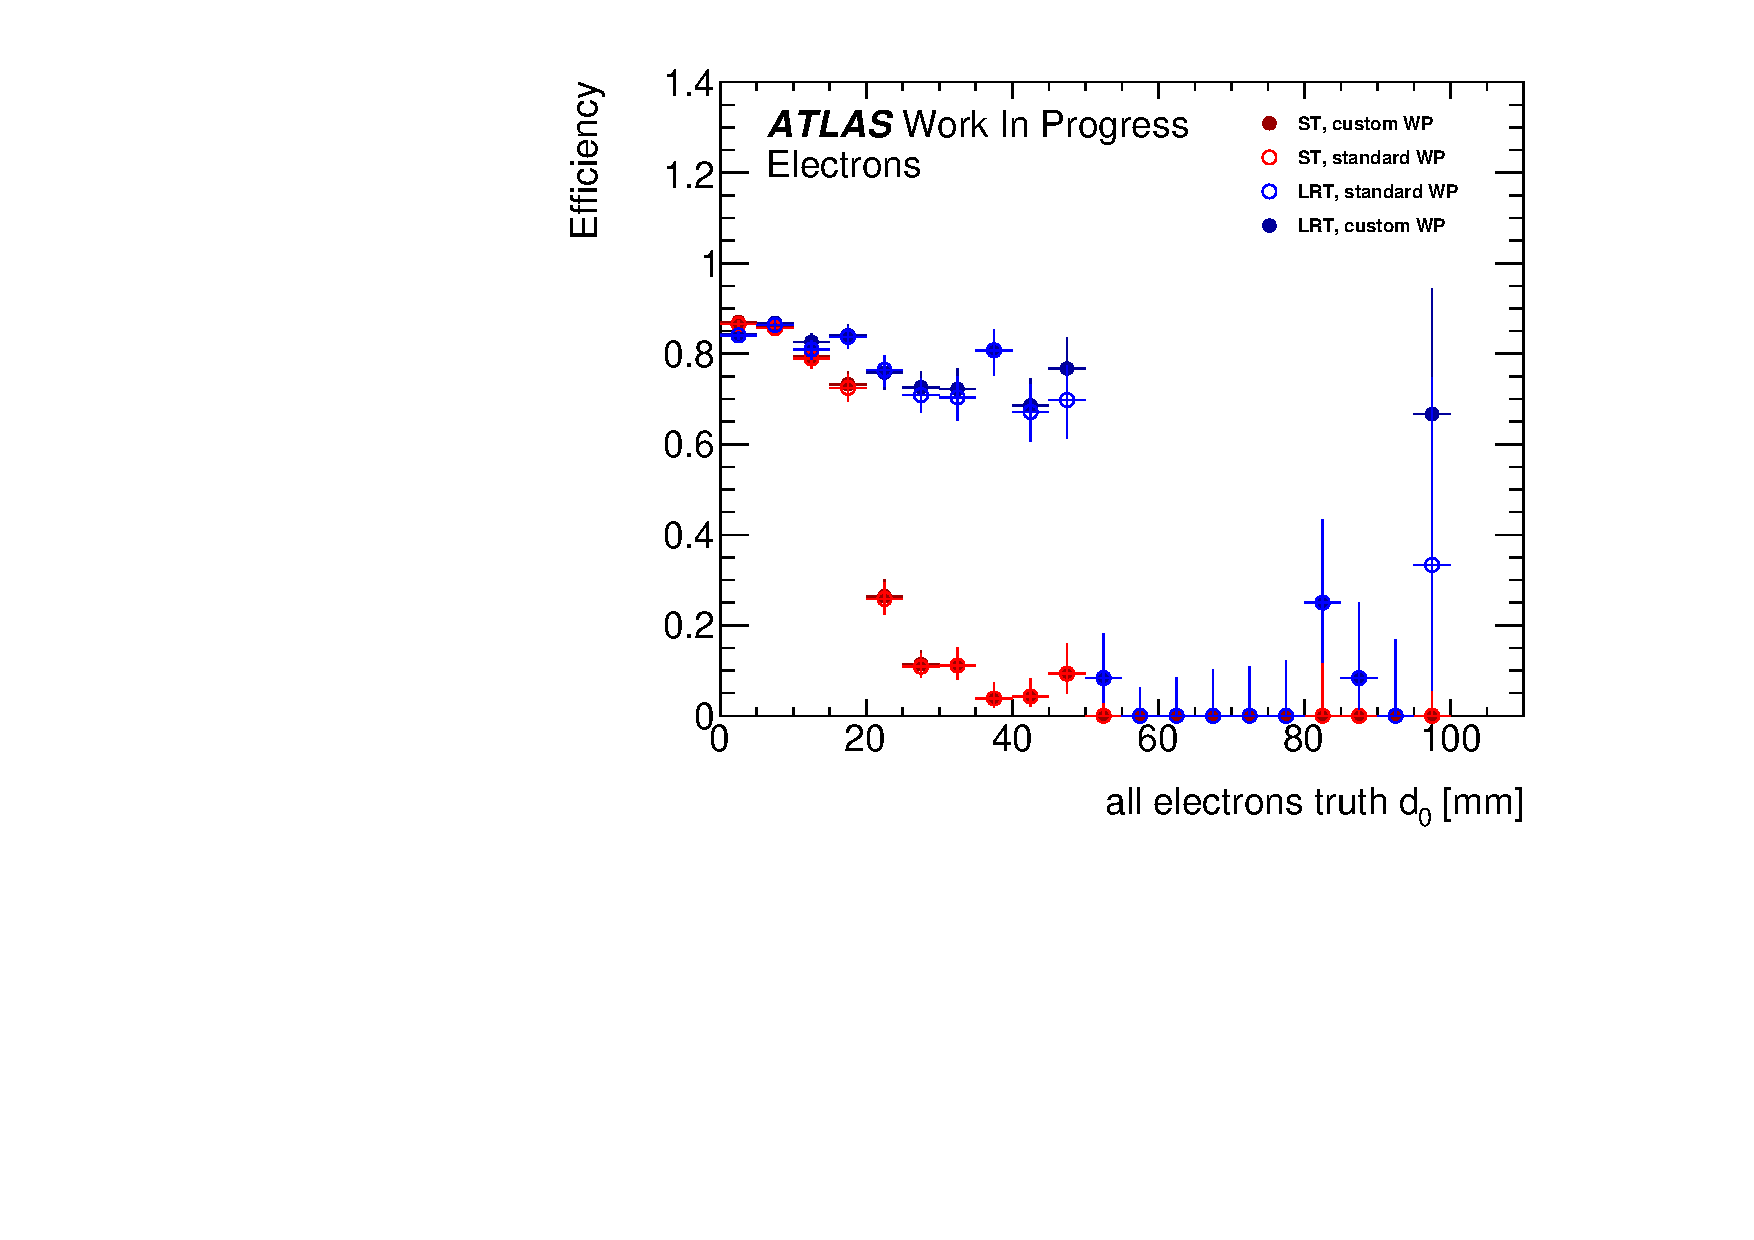
\includegraphics[width=.48\textwidth]{figures/EventReconstruction/wp_e_d0_all_wip.pdf}
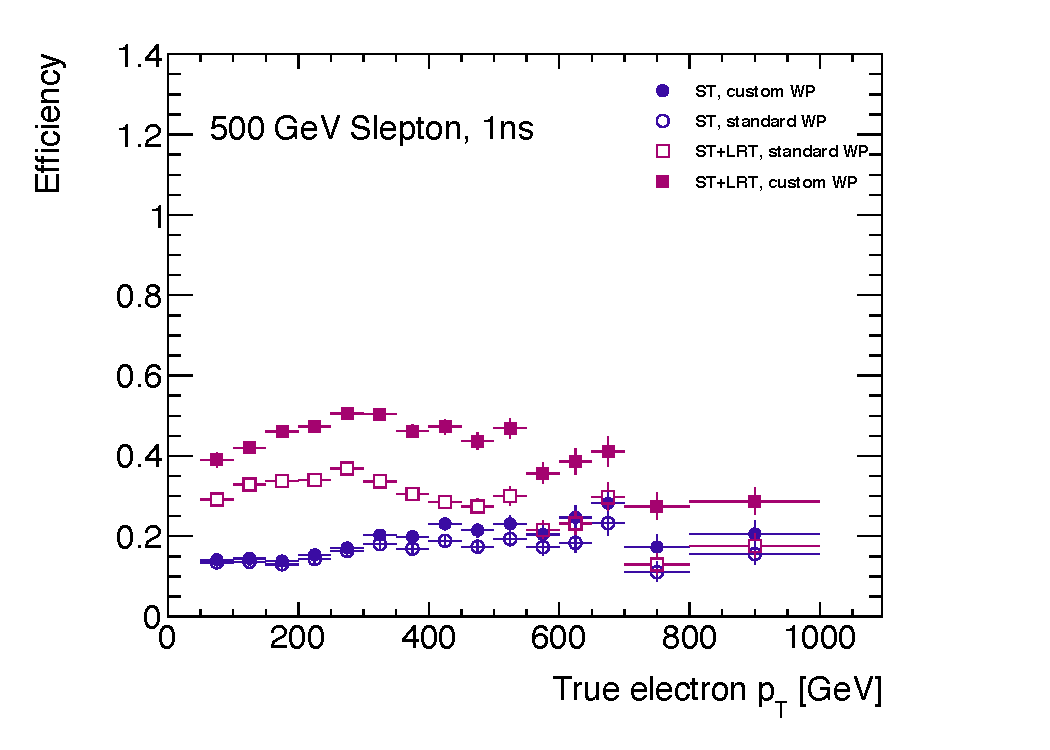
\includegraphics[width=.48\textwidth]{figures/EventReconstruction/wp_e_pt_all_wip.pdf}
\caption{Muon identification efficiency with modified criteria. Left is efficiency vs $d_{0}$ and right is efficiency as a function of $p_{T}$. The red denotes reconstruction with Standard Tracking (ST), and the blue with Large Radius Tracking (LRT), and the filled in circles use the modified identification working point. \todo{Needs update when available}}
\label{fig:cust_elec_eff}
\end{figure}




\section{Isolation}

In this analysis, both muons and electrons are required to be isolated to reduce background from heavy flavor decays. That is, they are not expected to be surrounded by much other activity from the hard scatter in either the Inner Detector or Calorimeters. Isolation is generally measured in terms as the scalar sum of energy in a radius $\Delta R = \sqrt{(\Delta \eta)^2 + (\Delta \phi)^2}$ around the lepton. Track based isolations are called $p_{T}^{\textrm{varcone}}$ and calorimeter based isolations called $E_{T}^{\textrm{topocone}}$. 

For example, the track-based isolation called $p_{T}^{\textrm{varcone30}}$ is the scalar sum of the transverse momenta of tracks with $p_{T} > 1 \GeV$ in a cone of $\Delta R = \textrm{min}(10 \GeV/p_{T}^{\ell}, 0.3)$, then a value is selected to determine what should be considered ``isolated''. Whereas the calorimeter-based isolation just counts the energy in a specified \dR, not as a function of the \pt of the particle. Isolation working points are then centrally defined as a combination of cuts on the track-based and calorimeter-based isolation. 

These definitions are much simpler for muons than for electrons. Electrons are very likely to emit bremsstrahlung radiation as they traverse the inner detector and those photons can then convert back into electrons. The tracks from these secondary particles are considered part of the electron's \pT. Furthermore, the electron leaves its own energy deposit in the \ac{EM} calorimeter and this energy must be subtracted from the $E_{T}^{\textrm{topocone}}$ calculation.


In this analysis we use the following working points \todo{grab isolation requirements from INT when finalized}


\section{Overlap Removal}
Each of the reconstruction chains described above, as well as those to reconstruction $\tau$ leptons, jets, and other physics objects used in \ac{ATLAS}, are run simultaneously. This means that the same track or cluster can be used to reconstruct two different types of physics objects. An iterative process of \ac{OR} is used to remove such artifacts. Overlap removal is performed on baseline objects, further described in \autoref{chap:event-selection}, which only pass identification and a loose \pt cut. 

Electrons $\dR < 0.01$ from a muon are removed to suppress contributions from muon bremsstrahlung radiation. Then, any baseline jet residing within $\Delta R < 0.2$ of a baseline electron is removed.  Baseline electrons with $E_{T}<50$~\GeV\ ($E_{T}>50$~\GeV) within $\Delta R < 0.4$ ($\Delta R < \mathrm{min}(0.4,0.04+10$~\GeV$/\pt)$) of any remaining jet are removed. The overlap removal procedure between muon and jet candidates is designed to remove muons that may originate from the decay of hadrons, with the overlapping jet being retained. Nearby jets may also occur as a result of high-\pt\ bremsstrahlung, in which case the jet should be removed and the muon retained. Such jets are removed if they reside within $\Delta R < 0.2$ of a baseline muon and have less than three matched inner detector tracks. Muons are removed if they reside within either $\Delta R < 0.4$ or $\Delta R < \mathrm{min}(0.4,0.04+10$~\GeV$/\pt)$ of any remaining jet, following the same \pt-dependent criteria as outlined for electrons above.




\cleardoublepage 

%----------------------------------------------------------------------------------------
\ctparttext{}
\part{Search for Displaced Leptons}

\chapter{Analysis Strategy}

\section{Target Models and Signal Regions}

\section{Overview of Backgrounds}

\section{Signal, Control, and Validation Regions}

\chapter{Event Selection}
\label{chap:eventselection}

\section{Analysis Strategy}

This analysis aims to select events that would have small cross sections producing only a handful of events from the entire 139 \ifb collected by \ac{ATLAS}. The signature of two displaced leptons, is rather simple in principle, but this analysis had not been done before in the conditions of the \ac{LHC}, so extensive optimization of the signal regions and lepton selection criteria needed to be done. A cut in the event selection should decrease or eliminate some background, but have little to no impact on the signal. For example, quality criteria ensure that leptons are well measured in the detector, and leptons from slepton decays will pass these quality criteria, but fake leptons from reconstruction failures generally will not. Every effort was made to remain as signal-agnostic as possible, so cuts on the specific topology of the \ac{GMSB} \ac{SUSY} decay were avoided. 

This analysis is split into three signal regions, defined by the flavor of the two highest \pt leptons in the event: SR-$ee$ with two electrons, SR-$\mu\mu$ with two muons, and SR-$e\mu$ with an electron and a muon. No requirement is placed on the charge of the leptons.
There are two definitions of leptons used: \emph{baseline} and \emph{signal}. Baseline leptons are required to pass the reconstruction and identification criteria described in \autoref{sec:el_reco_mods} and \autoref{sec:mu_reco_mods} and have $\pt > 50 \GeV$ and $\absdz > 2$ mm. Signal muons are required to further pass bespoke quality requirements, an isolation cut, and have $\pt > 65 \GeV$ and $\absdz > 3$ mm. Displacement-independent quality variables, described in the rest of this chapter, were defined specifically for this analysis as many standard quality criteria place requirements on the \absdz, \absz, or the number of hits in the Pixel detector, all of which would limit the ability to target displaced leptons.

\subsection{Background Overview}
The two signal leptons are required to have high \pt and high \absdz, higher than that expected of any leptons resulting from \ac{SM} processes. The remaining backgrounds come from failures of reconstruction algorithms, extreme tails of decays of \acf{HF} physics (b-jets or $\tau$s), and muons from cosmic rays. None of these background sources are well modeled in \ac{MC}, so data-driven methods must be used. This brings additional challenges from statistical limitations and care must be taken to avoid unblinding the signal regions.

Fake leptons result from the mis-association of a track to a calorimeter or \ac{MS} signature, creating a reconstructed lepton that does not correspond to a real particle that passed through the detector. 
This is particularly likely due to use of \ac{LRT}. The extended tracking algorithm loosens several requirements that enable high-\absdz tracking, but also introduces many \emph{fake tracks}, combinations of hits that do not correspond to the trajectory of a particle in the detector. When matched to \ac{MS} or calorimeter signatures, high-\absdz leptons can be created and form a background to this search. This is particularly likely to occur during electron reconstruction, where the track can be associated to real calorimeter signatures from photons or converted photons. 

The background to SR-$\mu\mu$ is dominated by cosmic ray muons. The \ac{ATLAS} detector is far underground partially to avoid the many particles from cosmic rays passing through the detector. However, there is a service shaft above the detector and muons can make it through the earth above the detector, so muons from cosmic rays are constantly passing through the detector. If a muon from a cosmic ray passes through the detector and is coincident with a bunch crossing, the event could be triggered and that muon reconstructed. Since it can pass at any point with respect to the collision, it can be reconstructed as one or two muons with high \absdz, exactly mimicking the targeted signature. 

Both electrons and muons suffer potential backgrounds from \ac{HF} decays, predominately from the decays of b-hadrons. b-quarks are very commonly produced in \ac{LHC} collisions and they immediately hadronize into b-hadrons, which have a lifetime of 1.5 ps and whose decays include a lepton 11\% of the time \cite{pdg}. This is sufficiently long that the b-hadron travels far enough before it decays such that a secondary vertex can be identified. Generally, the tracks have low \pt and maximum \absdz of about 1.5 mm, and the 3 mm cut on signal leptons is designed to minimize this effect. However, it is possible that extreme tails of this distribution are not well modeled in \ac{MC} and in an analysis where 0 background events are expected, understanding each possible source is paramount.


\section{Event Requirements}

Events must pass a trigger in order to be recorded by the \ac{ATLAS} detector. Three different triggers are used in this analysis and the data separated into three orthogonal regions based on the topology of the event, described in \autoref{tab:triggers}. The trigger is required to pass in the appropriate region for the event to be selected.

Each event is required to pass a standard set of \ac{ATLAS} event quality preselection criteria. Specifically, these include detector error flags which reject events with noise bursts or data corruption, or events in periods where any sub-detector was operating suboptimally. Events are required to have at least one \ac{PV} with $|z| < 200$ mm.

From events that pass the previous two requirements, events are sorted into the three signal regions based on the highest \pt baseline leptons in the event. Leptons in signal events are required to be well separated with $\dR_{\ell\ell} > 0.2$. This eliminates background from lepton pairs that could be created from an interaction with the material of the detector. Finally, signal events are required to have zero cosmic muons. The cosmic tag and the associated background will be discussed in \autoref{sec:cosmics}. The analysis was optimized and the backgrounds estimated while keeping the \acp{SR} blinded, so \acp{CR} (where backgrounds are estimated) and \acp{VR} (where additional studies and validation are done) are defined with different numbers of leptons and cosmic tags. All \acp{CR} and \acp{VR} are designed to be dominated by backgrounds and have very few signal events in them. A full list of all signal, control, and validation regions can be seen in \autoref{tab:regions}. 


\begin{sidewaystable}[!ht]
\small
\begin{center}
\begin{tabular}{l|l|c|c|c}
Purpose & Name & \# of Leptons & \# of Cos.Tags & Additional Requirements\\
\hline
%\multicolumn{5}{|c|}{Signal Regions} \\
%\hline
\multirow{3}{*}{Signal Regions} & SR-$ee$ 	& $\geq$ 2 $e$ 						& 0  & \\
								& SR-$\mu\mu$ & $\geq$ 2 $\mu$ 					& 0  & \\
								& SR-$e\mu$ 	& $\geq$ 1 $e$, $\geq$ 1 $\mu$  & 0  & \\
\hline
\multicolumn{5}{c}{Control Regions} \\
\hline
\multirow{2}{*}{Fake Estimation} 	&CR-$ee$-fake		& $\geq$ 2 $e$					& 0		& $\geq$ 2 loosened electrons, not in SR-$ee$  \\
									&CR-$e\mu$-fake		& $\geq$ 1 $e$, $\geq$ 1 $\mu$ 	& 0		& $\geq$ 2 loosened leptons, not in SR-$e\mu$  \\
\hline
Heavy Flavor Estimation 			&CR-$\mu\mu$-hf		& $\geq$ 2 $\mu$				& 0 	& $\geq$ 1 anti-isolated $\ell$, loosened \pt and \dz \\
\hline
\multirow{2}{*}{Cosmic Estimation} 	&CR-$M_{\mathrm{full}}$  & $\geq 1 \mu$		& $\geq 1$ 	    &  includes muons failing \nphi and \nprecision cuts\\
									&CR-$\mu\mu$-topbad	& $\geq$ 2 $\mu$				& 0  	& one signal and one loosened muon \\
\hline
\multicolumn{5}{c}{Validation Regions} \\
\hline
\multirow{4}{*}{Cut Evaluation}		&VR-$M_{\mathrm{narrow}}$& $\geq 1 \mu$		& $\geq 1$ 	& using narrow cosmic tag \\ 
									&VR-$e$					& 1 $e$, 0 $\mu$	& 0 		& electron is baseline  \\
									&VR-$\mu$				& 0 $e$, 1 $\mu$	& 0 		& muon is baseline  \\   
% evaluating cleaning cuts
\hline
\multirow{4}{*}{Fake Validation}	&VR-$ee$-fake			& $\geq$ 2 $e$					& 0 & inverted \dpt selection \\
									&VR-$ee$-fake-hf		& $\geq$ 2 $e$					& 0 & $\geq 1$ anti-isolated $\ell$, loosened quality  \\
									&VR-$e\mu$-fake			& $\geq$ 1 $e$, $\geq$ 1 $\mu$ 	& 0 & 1 $e$ fails \dpt, 1 $\mu$ fails \chiCB \\ 
									&VR-$e\mu$-fake-hf		& $\geq$ 1 $e$, $\geq$ 1 $\mu$	& 0 & 1 $e$ fails \dpt, no isolation req., loosened quality \\
% Validation of fake estimates, including HF contribution
\hline
\multirow{3}{*}{Cosmic Validation}	&VR-$\mu M_{\mathrm{full}}$  & $\geq$ 2 $\mu$			& 1 	& \\		
									&VR-$\mu$-narrow 			& $\geq$ 1 $\mu$			& 0* 	& using narrow cosmic tag \\
									&VR-$\mu M_{\mathrm{narrow}}$& $\geq$ 2 $\mu$			& 1* 	& using narrow cosmic tag \\
% Validation of cosmics

\hline
\end{tabular}
\caption{Summary of signal, control and validation regions used in the analysis. All regions are defined exclusively by their reconstructed leptons. In the table, all leptons should be assumed to be signal leptons except for their noted deviation from the signal requirements. All requirements are placed on the two leading leptons, additional leptons are allowed in the event but no selections are made on them. In each region, the appropriate trigger selection is made. In region names, a capital $M$ denotes a cosmic-tagged muon, and for requirements on numbers of cosmics, all leptons in the event are considered. An * on the number of cosmic tags denotes the number of muons tagged or untagged by the narrow tag, not the nominal tag used in the signal regions.}
\label{tab:regions}
\end{center}
\end{sidewaystable}



\section{Electrons}

Quality cuts specifically designed for this analysis are introduced to eliminate fake electrons reconstructed from the incorrect association of tracks and calorimeter clusters. The most important of these cuts is 
\begin{equation}
\dpt \equiv \frac{p_{T, \text{track}} - p_{T, e}}{p_{T, e}}
\end{equation}
which measures the degree of consistency between the \pt of the electron, which is dominated by the calorimeter measurement, and the \pt of the track. Fake tracks tend to be low \pt, resulting in fake electrons with tracks with less than half of the \pt of the electron, $\dpt < -0.5$,.

Additionally, quality requirements are imposed on the \ac{ID} tracks. They are required to have $\chiID < 2$ \footnote{In this thesis, $\chi^{2}$ implies $\chi^{2}$ divided by the number of degrees of freedom in the fit} and no more than 1 missing hit after the first hit in the track. These cuts remove poor hit combinations, short tracks, or tracks missing measurements. Additionally, signal electrons are required to be isolated and pass the \texttt{FCTight} isolation definition described in \autoref{sec:isolation}

\begin{table}[!ht]
\begin{center}
\begin{tabular}{c|c}
\multicolumn{2}{c}{Electron Selections}\\
\hline
\pt & $> 65~\gev$ \\
\absdz & $> 3$ mm \\
$|\eta|$ & $< 2.47$ \\
Isolation & \texttt{FCTight} \\
\dpt & $\geq$ -0.5 \\
\chiID & $< 2$ \\
\nmiss & $\leq$ 1 \\ 
\hline
\end{tabular}
\caption{Overview of electron signal selections.}
\label{tab:electron_sel}
\end{center}
\end{table}


\section{Muons}

Signal muon requirements are similar to those placed on signal electrons. The muon is required to have $\chiCB < 3$ in order to ensure a good combination between \ac{ID} track and \ac{MS} track, similar to the \dpt cut on electrons. Additionally, signal muons are required to pass the same \ac{ID} track quality requirements as electrons as well as \ac{MS} track quality requirements. Requiring $\nprecision \geq 3$ (number of \ac{MDT} layers with at least 3 hits) and $\nphi \geq 1$ (number of \ac{RPC} hits) ensure that the \ac{MS} track is well measured in both its $\eta$ and $\phi$ coordinates. Signal muons required to pass the \texttt{FCTight} isolation requirement described in \autoref{sec:isolation}. 

Furthermore, muons are required to have $\tavg < 30$. \tavg is the average $t_{0}$ calculated from the \ac{MS} segments associated to the muon. The measurement of $t_{0}$ is described in \autoref{sec:mdt-timing}. If the fit fails, the segment is assigned $t_{0} = 0$, and this value does not enter the \tavg calculation, but muons that have all segments with $t_{0} = 0$ are not rejected. This cut is designed to better control the background from cosmic muons, which have a much wider spread in \tavg than collision muons.

\begin{table}[!ht]
\begin{center}
\begin{tabular}{c|c}
\multicolumn{2}{c}{Muon Selections}\\
\hline
\pt & $> 65~\gev$ \\
\absdz & $> 3$ mm \\
$|\eta|$ & $< 2.5$ \\
Isolation & \texttt{FCTight} \\
\nprecision & $\geq$ 3 \\
\chiCB & $< 3$ \\
\nphi  & $ \geq 1$ \\
\chiID & $< 2$ \\
\nmiss & $\leq$ 1 \\
$|\tavg|$ & $< 30$ \\
Pass Cosmic Veto & True \\
\hline
\end{tabular}
\caption{Overview of muon signal selections.}
\label{tab:muon_sel}
\end{center}
\end{table}




\section{Acceptance and Efficiency}

Acceptance is defined as the fraction of events that could enter the \ac{SR} based on their kinematics, and efficiency is fraction of the accepted events that get correctly identified. The acceptance and efficiency in this analysis are both rather low. The exponential nature of the \pt and \absdz distributions of the \slep decays, many daughter leptons have low \pt and low \absdz and do not pass the signal kinematic selections and are not accepted. This particularly effects low mass, low lifetime \slep; the \pt cut has an even stronger impact on leptons from \stau decays, which must decay through a standard model $\tau$. Conversely, the degradation of the \ac{LRT} efficiency at high \absdz means that leptons with high \absdz are often not reconstructed. This particularly effects \slep with long lifetimes. Additionally, the \pt and \absdz and $\eta$ cuts required to pass one of the triggers used in this analysis to pass the \ac{LRT} filters further reduces the acceptance and efficiency.

The acceptance is highest for lifetimes around 0.1 ns, around 30\% for \smu and \selec production and only 0.5\% or \stau production. The efficiency is higher, around 50\% for lifetimes of order 0.1 ns for all flavors of \slep. The values for a range of possible mass and lifetime points can be see in \autoref{fig:acc-eff-mm}, \autoref{fig:acc-eff-ee}, \autoref{fig:acc-eff-em}

\begin{figure}[htbp]
\centering
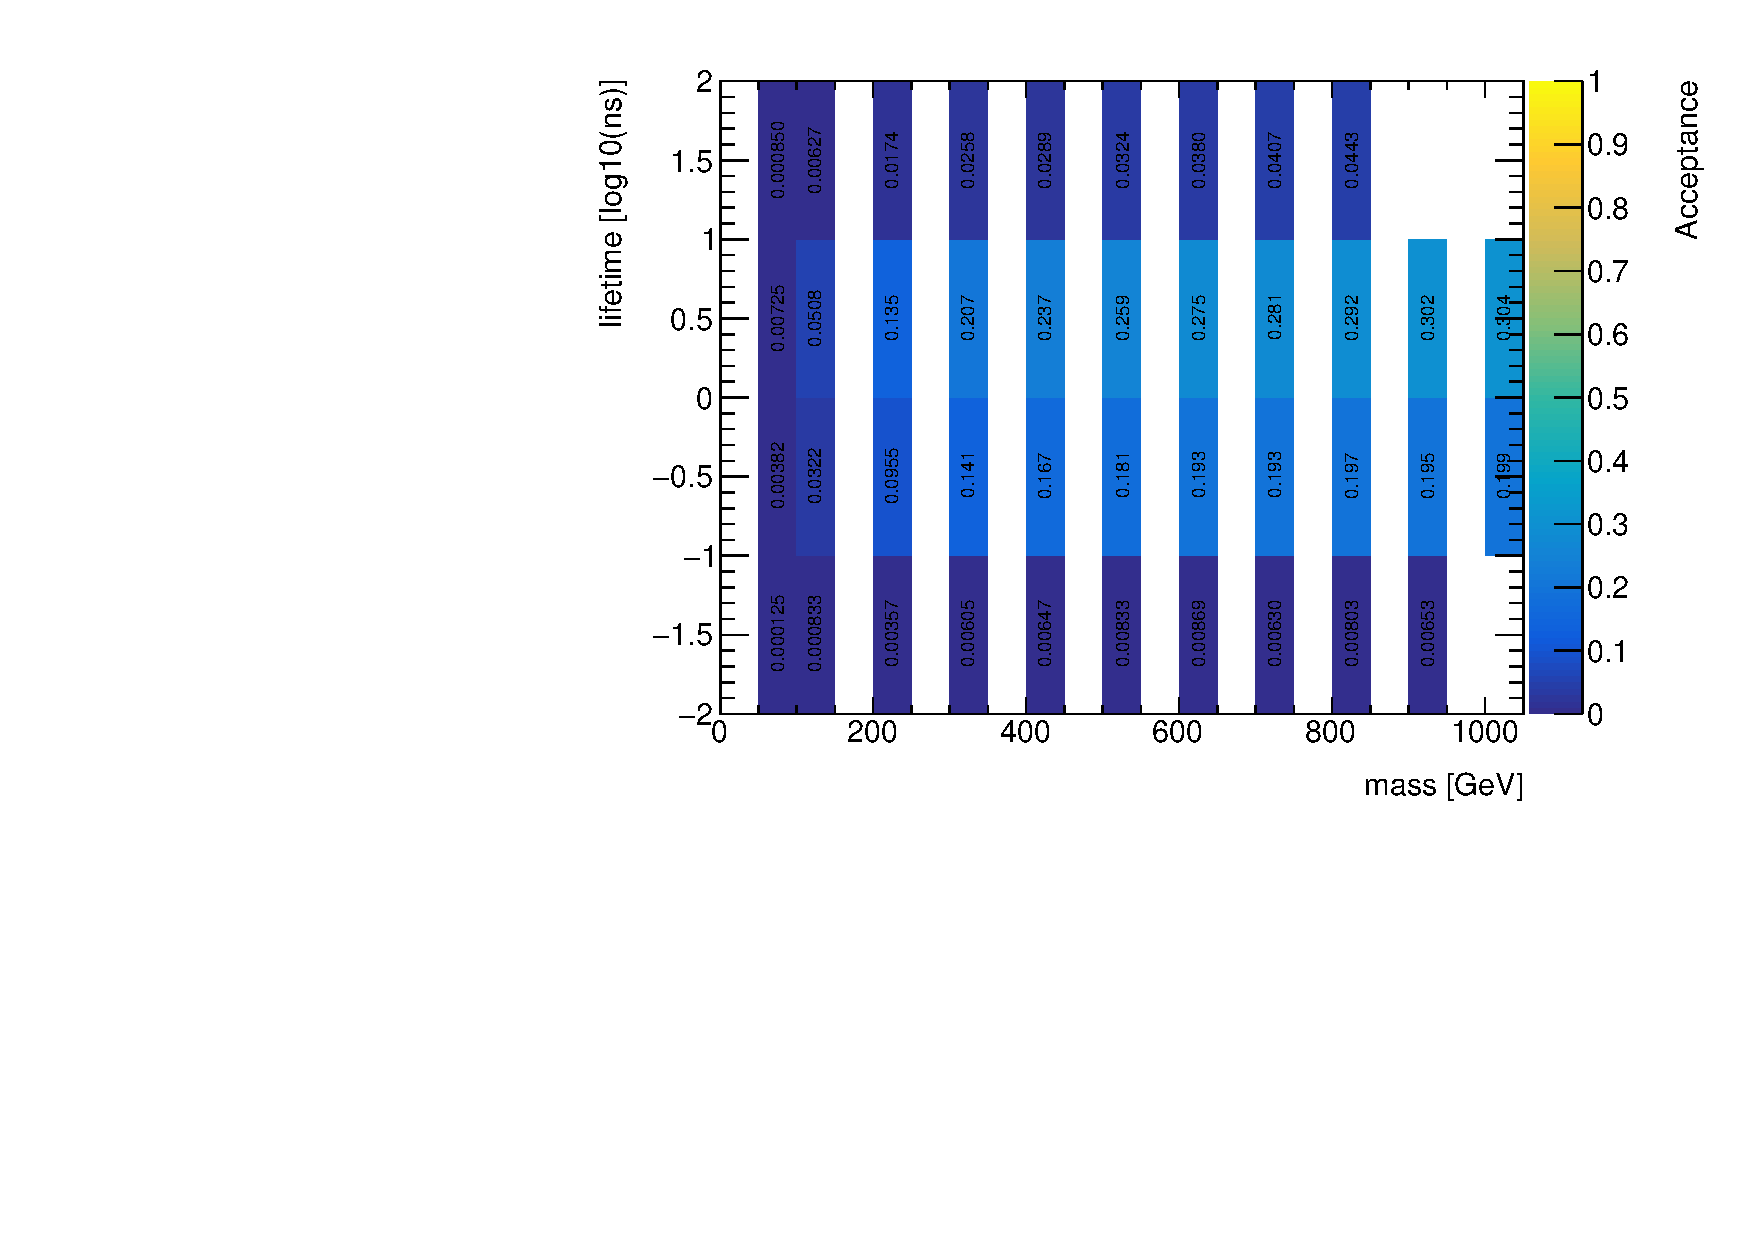
\includegraphics[width=.48\textwidth]{figures/event_selection/mm_slep_acc.pdf}
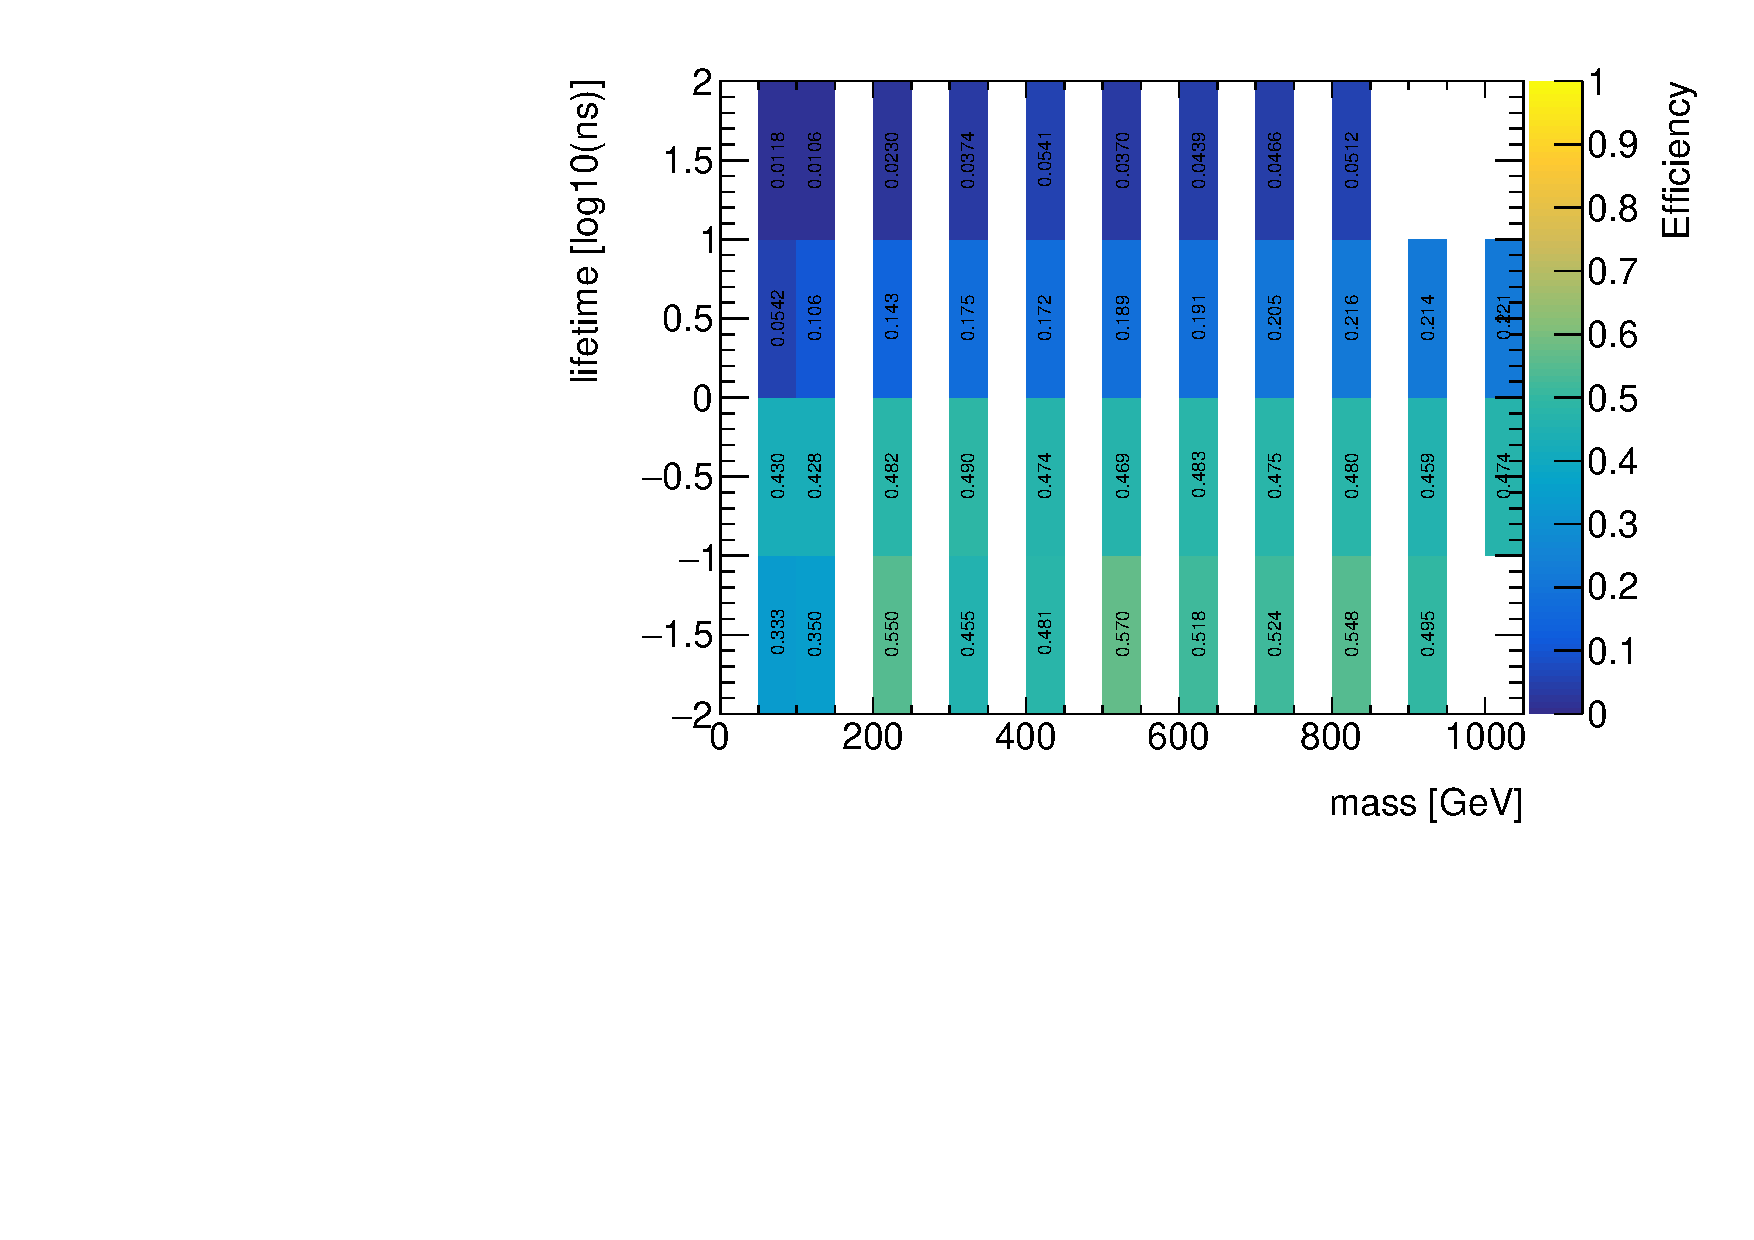
\includegraphics[width=.48\textwidth]{figures/event_selection/mm_slep_eff.pdf}
\caption{Acceptance (left) and efficiency for \smu decaying to muons in SR-$\mu\mu$. The x-axis shows the possible masses of the \smu and the y-axis its possible lifetime.}
\label{fig:acc-eff-mm}
\end{figure}

\begin{figure}[htbp]
\centering
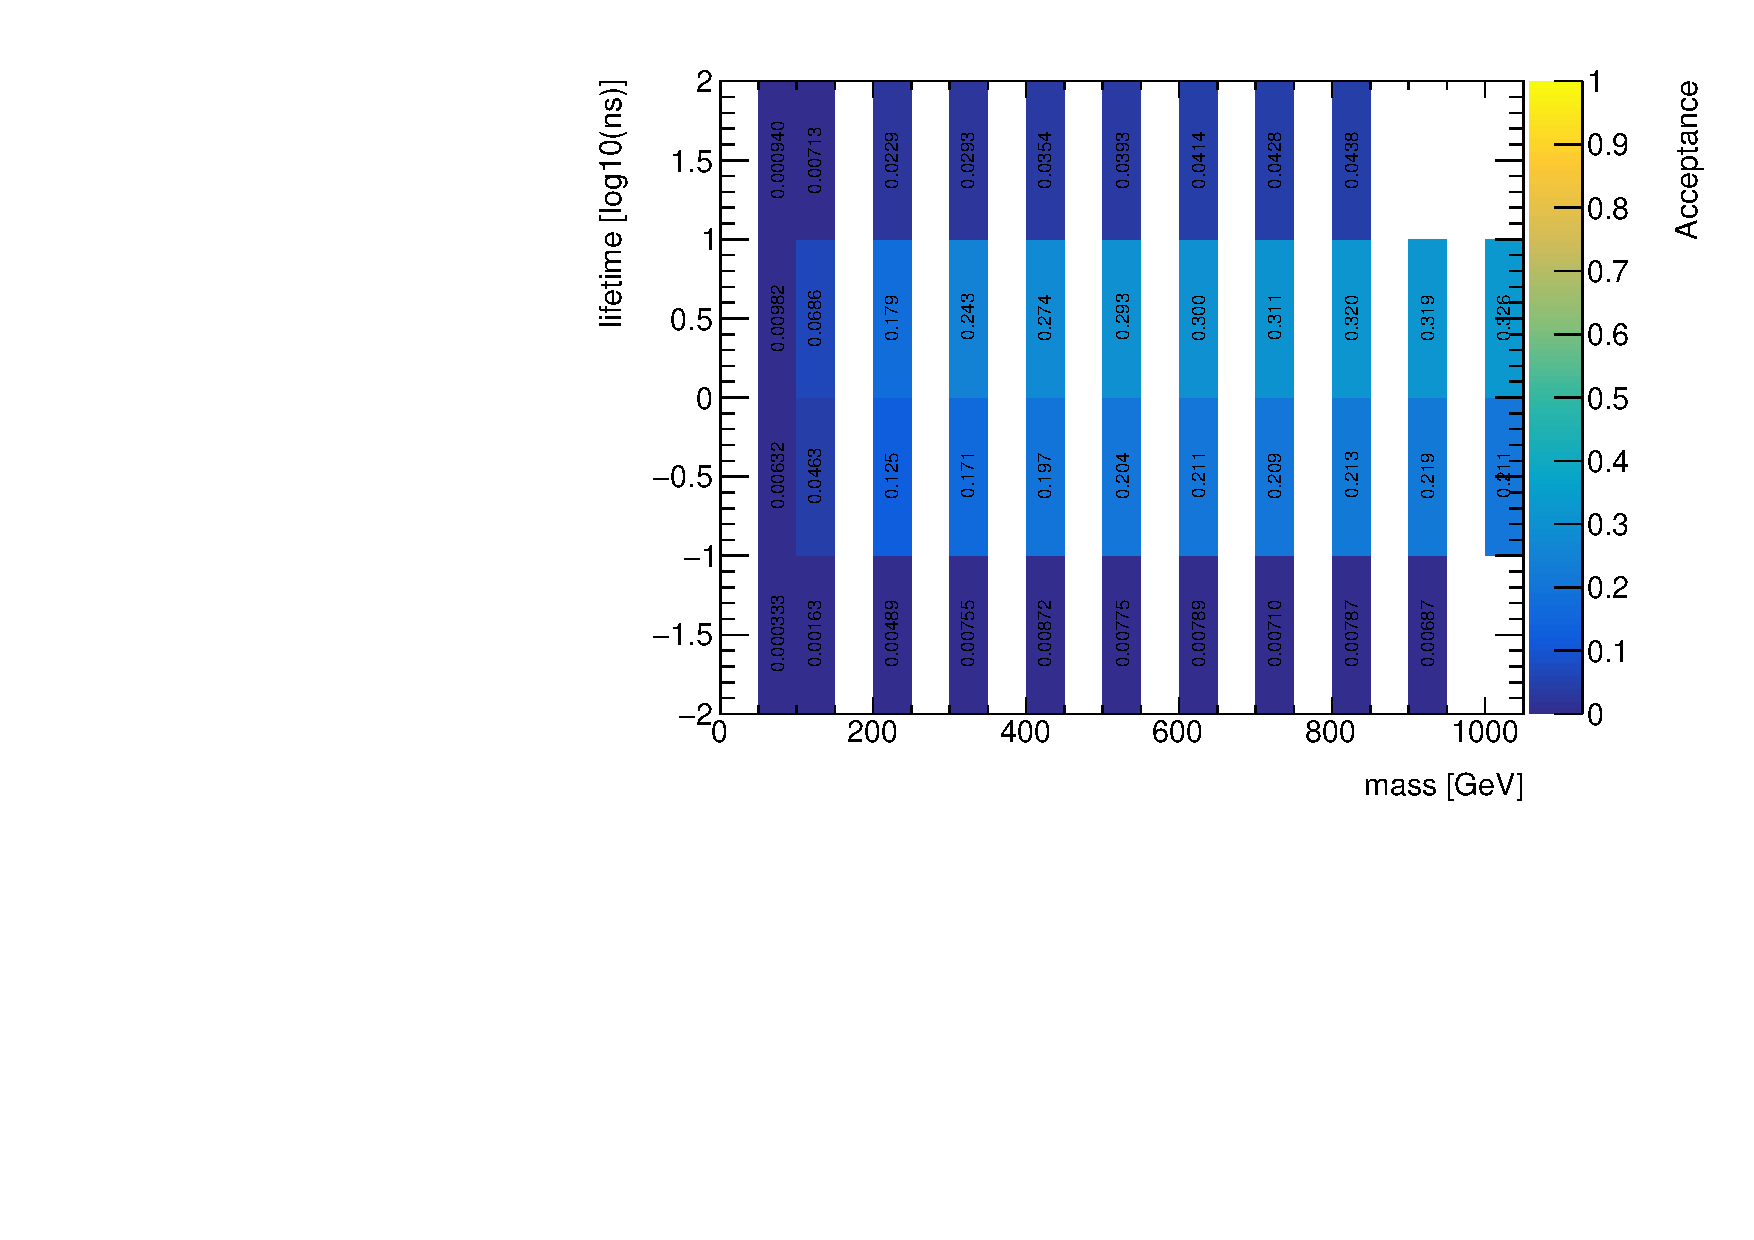
\includegraphics[width=.48\textwidth]{figures/event_selection/ee_slep_acc.pdf}
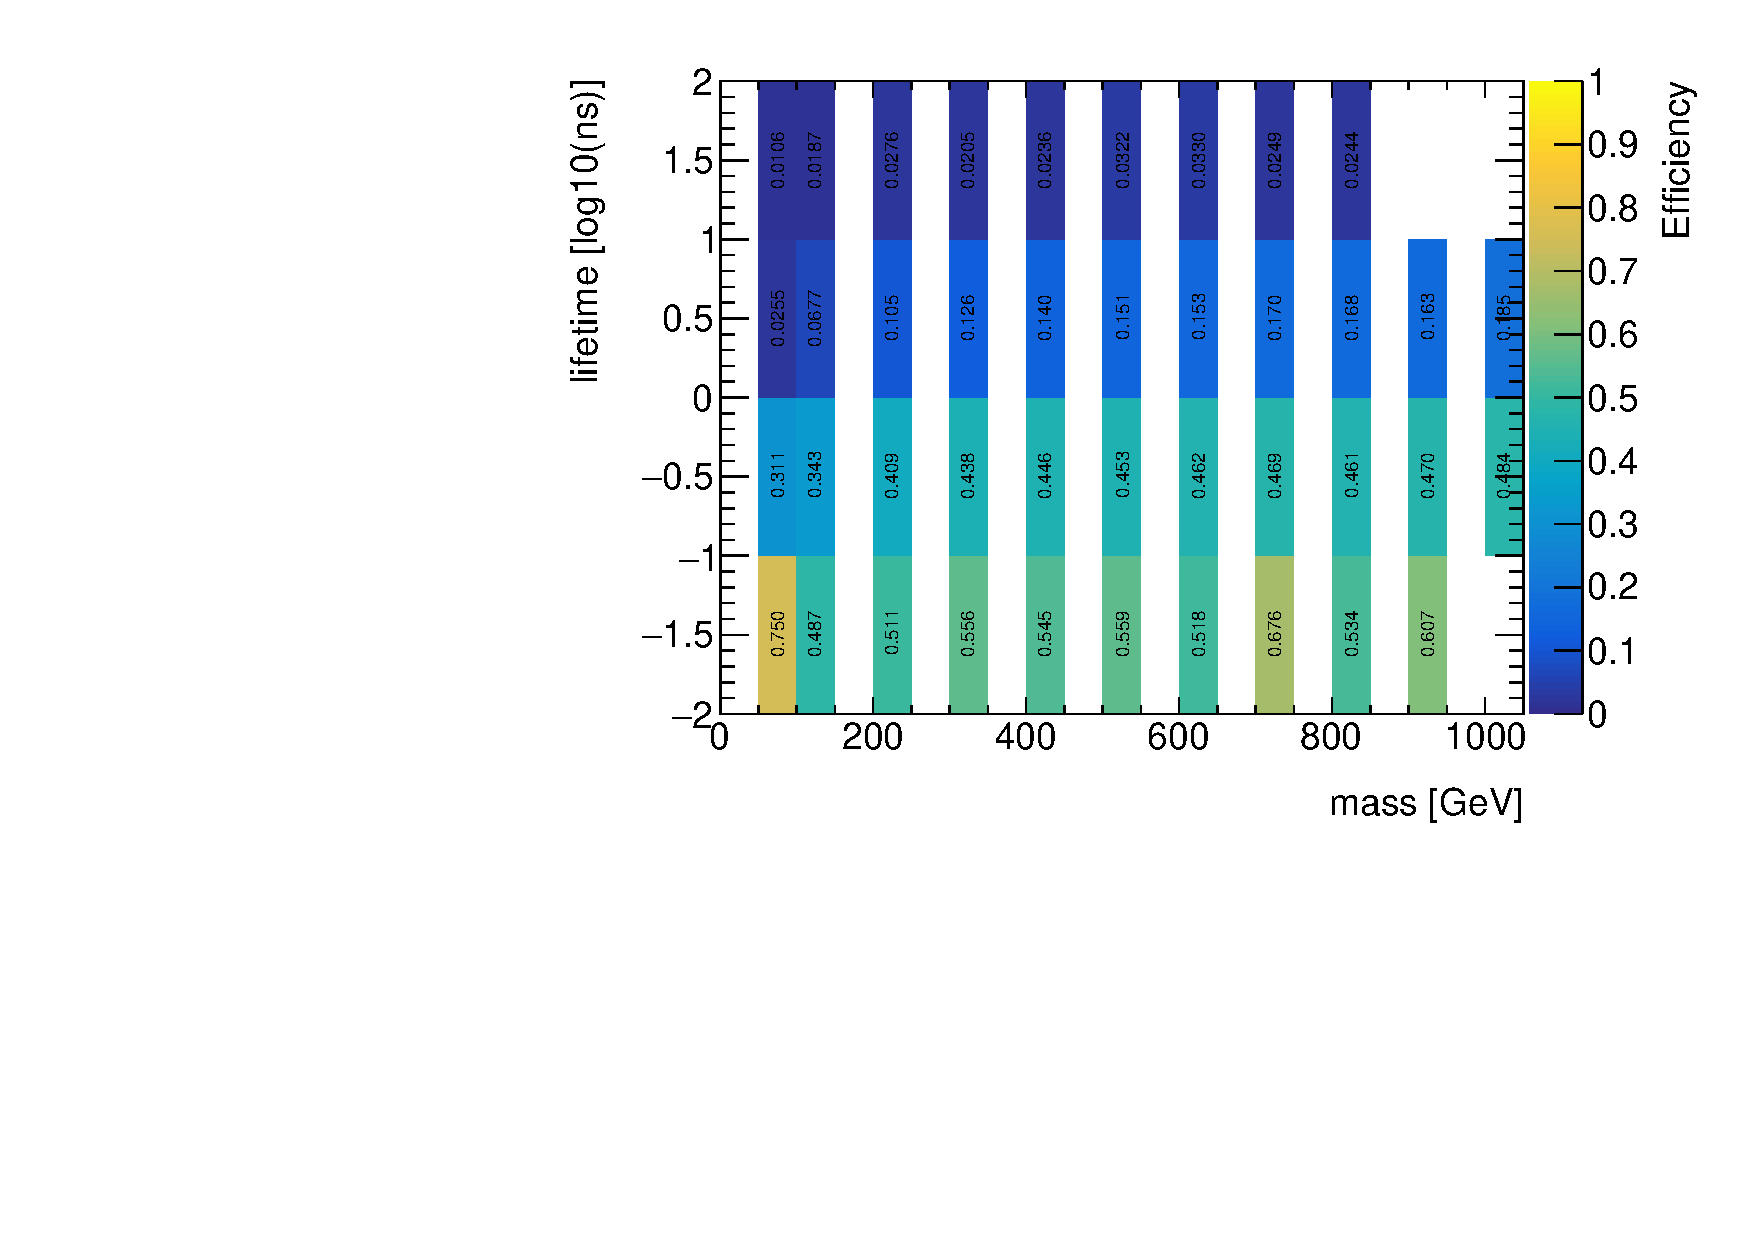
\includegraphics[width=.48\textwidth]{figures/event_selection/ee_slep_eff.pdf}
\caption{Acceptance (left) and efficiency for \selec decaying to electrons in SR-$ee$. The x-axis shows the possible masses of the \selec and the y-axis its possible lifetime.}
\label{fig:acc-eff-ee}
\end{figure}

\begin{figure}[htbp]
\centering
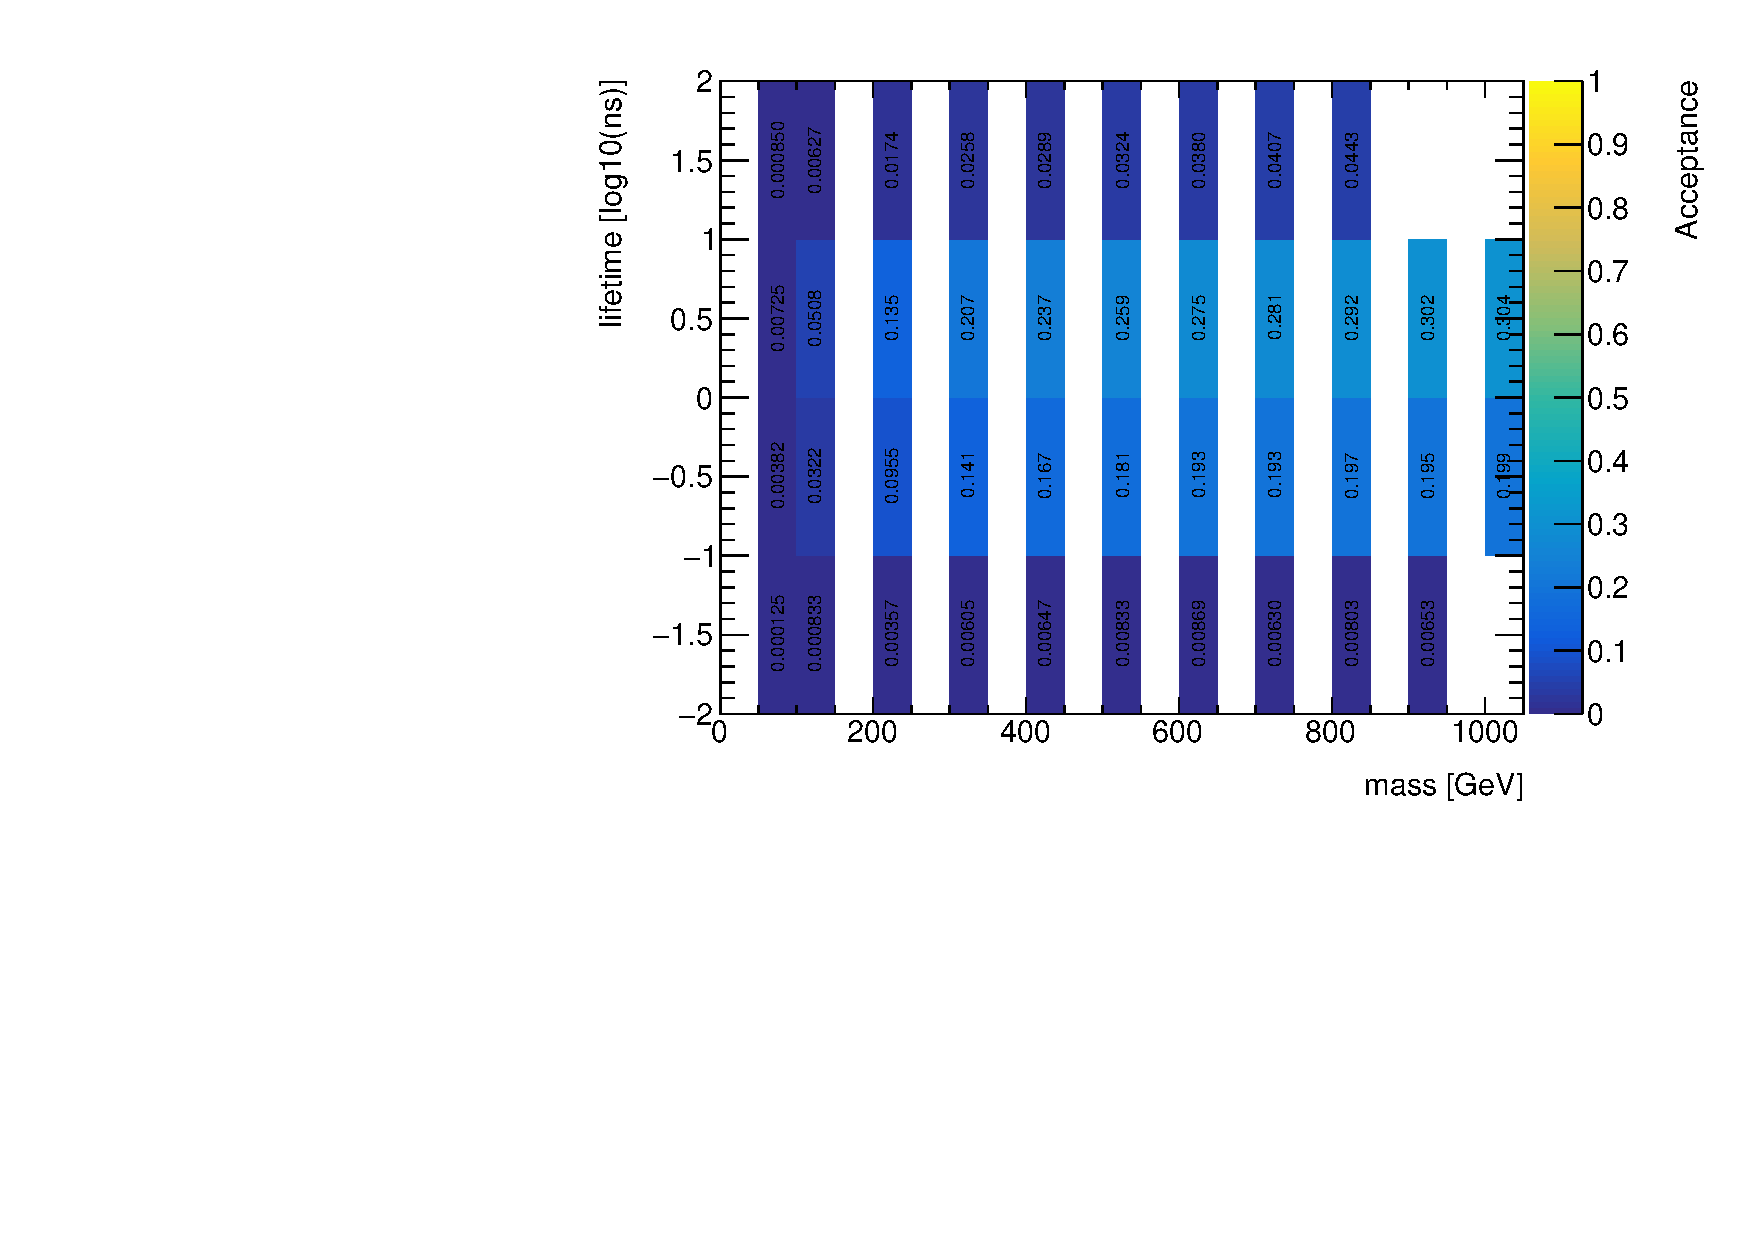
\includegraphics[width=.48\textwidth]{figures/event_selection/mm_slep_acc.pdf}
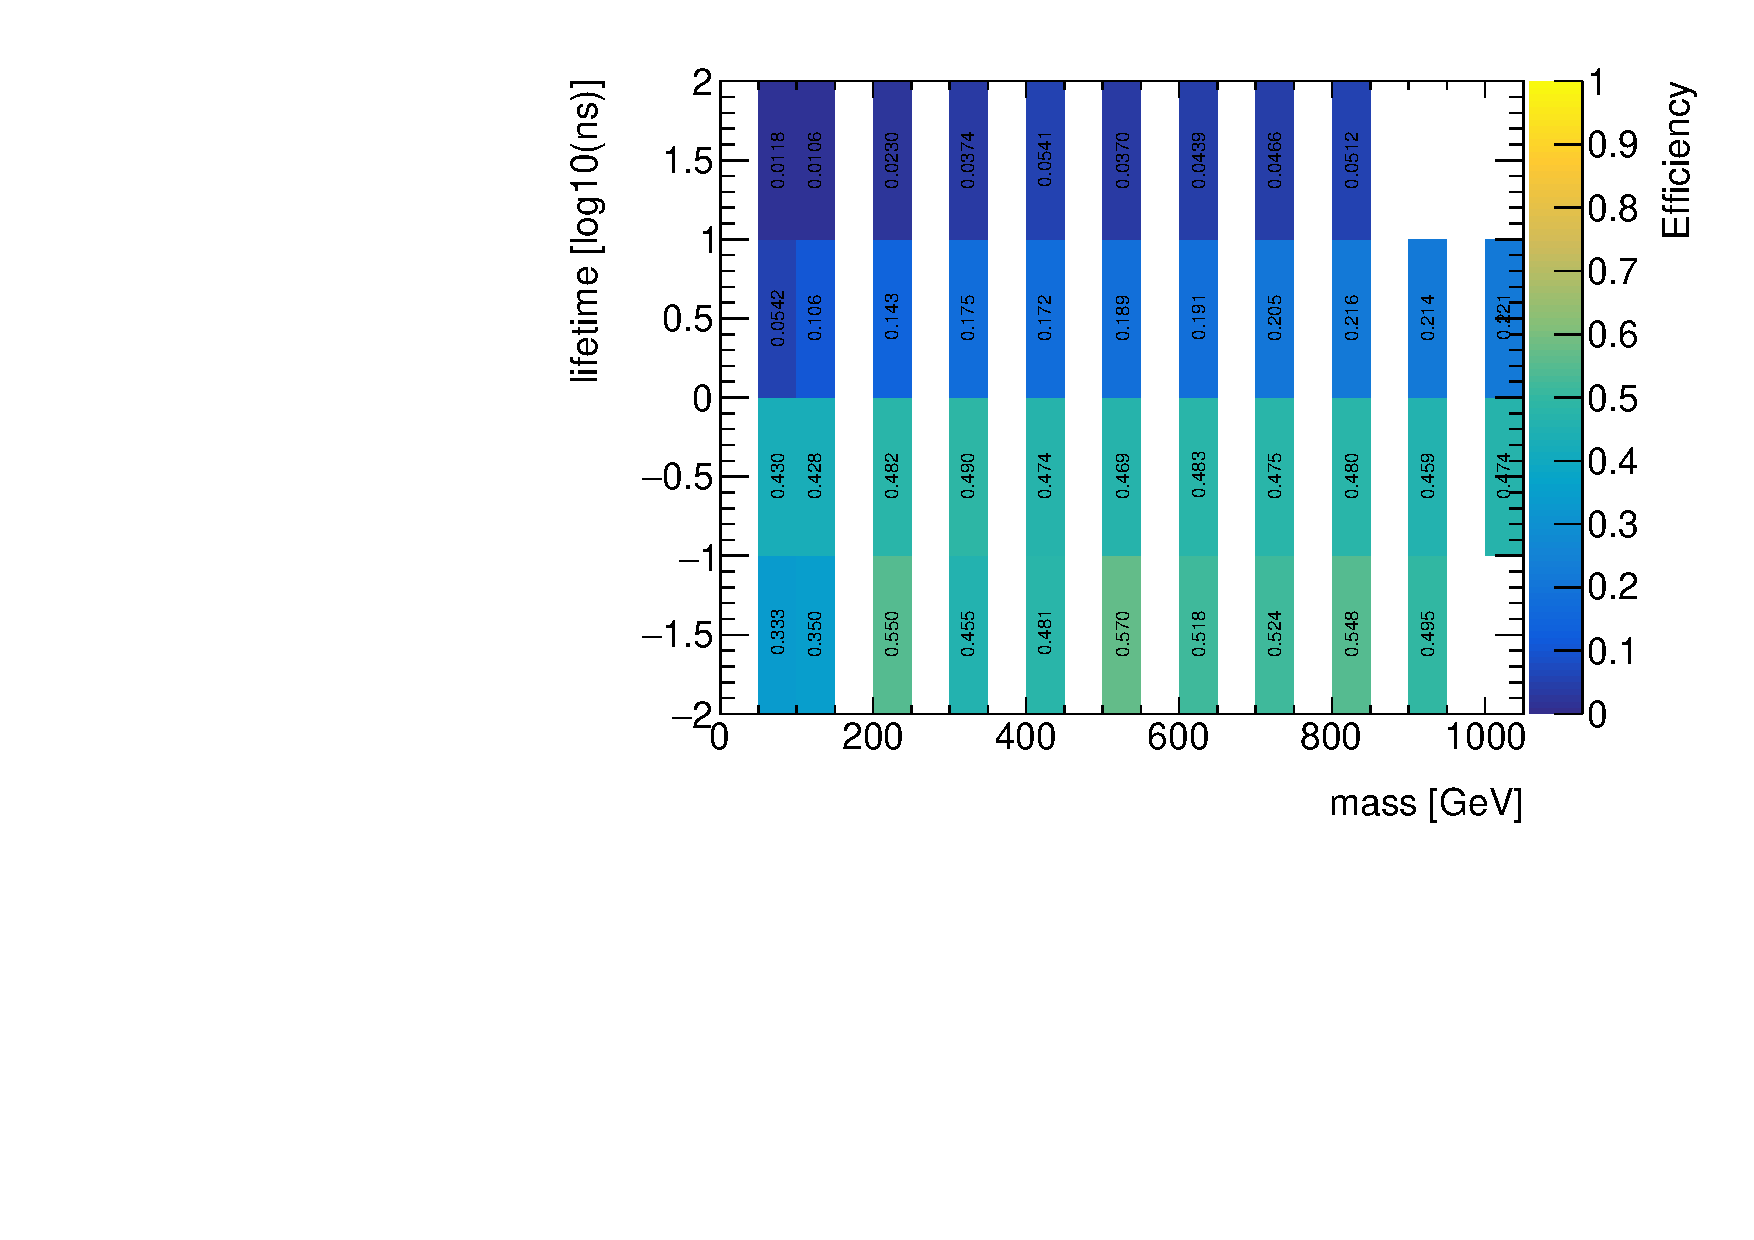
\includegraphics[width=.48\textwidth]{figures/event_selection/mm_slep_eff.pdf}
\caption{Acceptance (left) and efficiency for \stau s decaying to taus in SR-$\mu\mu$, SR-$ee$, and SR-$e\mu$ combined. The x-axis shows the possible masses of the stau and the y-axis its possible lifetime.}
\label{fig:acc-eff-em}
\end{figure}





\chapter{Backgrounds}
\label{chap:backgrounds}

In this analysis, backgrounds are estimated per signal region. In SR-$ee$ and SR-$e\mu$, algorithmic fakes are the dominant source of background. In SR-$\mu\mu$, the background contribution from algorithmic fake muons and muons from heavy flavor decays is negligible ($\mathcal{O}(10^{-4})$), and the dominant background is from cosmic muons coincident with \ac{LHC} collisions. While the signal lepton selection and event selection described in the previous chapter very efficiently remove these backgrounds, background estimates are calculated to estimate any residual contribution. All backgrounds are not well modeled in \ac{MC}, so must be estimated from \acp{CR} in data, often resulting in statistical limitations.

\section{Background to SR-$ee$}

\subsection{Fakes and Heavy Flavor Decays}

The primary background to SR-$ee$ is algorithmic fakes from the misassociation of a track with a real energy deposit in the \ac{EM} calorimeter (such as from a photon); there is a secondary contribution from electrons from \ac{HF} decays. \ac{MC} samples of \ttbar along with a photon dominated sample (described in \autoref{sec:mc}) were used to study the relative contributions. 

The \ttbar provides a sample of \ac{HF} decays (though not the dominant source of \ac{HF} decays at the \ac{LHC}), yet after all of the signal requirements, the remaining high \absdz electron was the result of a photon combined with an \ac{ID} track. That this sample has many more b-hadron decays than photons, yet the photons contribute a larger background even in this narrow region of phase space, indicates that algorithmic fakes are the larger contributer of background events to SR-$ee$. Additionally, in truth-level studies of background \ac{MC}, such as \bbmm (at truth level, the electron and muon kinematics are the same), $Z\rightarrow \tau\tau$ (where the $\tau$ decays include electrons), and \ttbar, all show exponentially falling distributions with no two lepton events that pass the \pt and \absdz cuts in the \ac{SR}, as designed. 

Further studies were performed in data, with one baseline electron passing the filter requirements and another lepton with no \absdz cut made. This second lepton must be \emph{anti-isolated}, meaning it fails the isolation requirement made on signal leptons and has substantial activity surrounding it in the calorimeter and/or the \ac{ID} and is likely to be inside of a jet. While the \dpt cut is designed to remove algorithmic fakes, it is a very effective remover of anti-isolated electrons as well. Clusters associated to electrons reconstructed inside of jets are likely to have additional energy incorrectly added to their clusters, increasing the cluster \pt and decreasing the \dpt. Thus, it is not possible to disentangle heavy flavor electrons from fake electrons and the background contributions are estimated together with fakes as the dominant contribution.


\subsection{Background Estimate}
Fake electrons result from the failure of the reconstruction algorithm algorithm, and so the two fake electrons in an event should be uncorrelated. This assumption is used to estimate the background with an \emph{ABCD method}. The procedure divides events into four regions based on the quality of the leading and subleading leptons in the event, shown in \autoref{fig:abcd}. The number of events in regions B, C, and D are combined to estimate the number of events in region A, the signal region:

\begin{equation}
N_A = \frac{N_B}{N_D}\times N_C
\end{equation}


\begin{figure}[!ht]
\centering
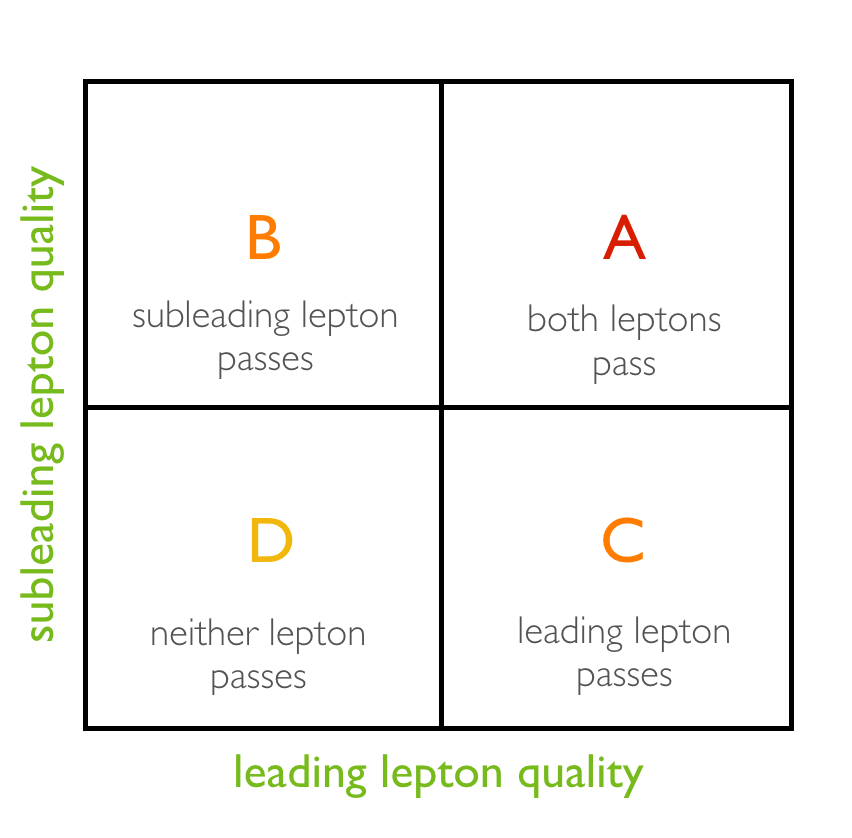
\includegraphics[width=.5\textwidth]{figures/otherbackgrounds/abcd.png}
\caption{The regions used for ABCD estimation.}
\label{fig:abcd}
\end{figure}


In the nominal estimate, region A is the signal region, with two electrons passing all signal cuts, region D has both electrons failing at least one signal cut, and regions C and D have only one electron passing all signal cuts while the other fails at least one (regions B, C, and D compose CR-$ee$-fake). For this estimate, a ``failing'' electron fails one of the \dpt, \chiID, or \nmiss requirements, while a ``passing'' electron is a signal electron, passing all three cuts. The number of events in each region and the estimated number of events in SR-$ee$ is shown in \autoref{tab:abcd_ee}.

\subsection{Validation and Systematic Uncertainties}
The definitions of the ABCD regions can be varied to perform validations of the estimate and quantify systematic uncertainties. There are two ways to do this: first, the estimate can be done in slightly different ways, and the difference from the nominal estimate taken as an uncertainity; second, an estimate can be done in a validation region, where one or more signal cuts are inverted, and the estimated number of events can be compared to the actual number of events in region A. In the second scenario, one looks for \emph{closure}, that the estimate correctly estimates the number of events (within statistical uncertainties), giving evidence that the method and its assumption are sound. If this is not the case, the \emph{nonclosure}, the extent to which the estimate disagrees with the correct number of events, is evaluated and an uncertainty can be taken to cover this.

\begin{table}[htb]
\small
\begin{center}
\begin{tabular}{lcc}
Region     & Nominal            & Only \dpt   \\
\hline
D Observed & 9068         & 1440      \\
C Observed & 77           & 28      \\
B Observed & 54           & 19      \\
A Estimate & $0.459 \pm 0.082$  & $0.37 \pm 0.11$   \\
\hline
\end{tabular}
\caption{Results of the ABCD estimate for the nominal SR-$ee$ estimate, the number of events in each region are shown as well as the estimate for A. The uncertainties are statistical only and using Poisson statistics.}
\label{tab:abcd_ee}
\end{center}
\end{table}

Validations are performed by estimating the number of events in SR-$ee$ in different ways. For example, only the \dpt, the most effective fake discriminator, is used as the ``passing''/``failing'' variable. The results of this estimate are also shown in \autoref{tab:abcd_ee}, the results are consistent within statistical uncertainties but the nominal estimate is more precise.

The second kind of validation is performed in two regions: one that enhances the fake contribution, and a second that enhances the \ac{HF} contribution. First, in a fake enhanced region, VR-$ee$-fake, where the \dpt cut is inverted and the estimate is performed with \chiID and \nmiss together as the ``passing''/``failing'' variables. This changes the estimate to predicting the number of fake electrons (failing \dpt) from regions with electrons that are more fake (failing \dpt and one or both of \chiID and \nmiss). In this region, 1440 events are observed, and 1356 $\pm$ 49 are predicted. Even though this result is consistent within the statistical uncertainties, the difference between the central values (6.2\%) is taken as a nonclosure and applied as a systematic uncertainty on the \ac{SR} estimate.

Next, a validation is done in a \ac{HF} enhanced region, VR-$ee$-fake-hf, which is identical to CR-$ee$-fake with the additional requirement that at least one electron is anti-isolated. This additional requirement reduces the statistics in the region quite a bit, so the electron cuts are loosened to $\pt>50\gev$, $\absdz > 2$ mm, and instead of the usual \dpt cut at -0.5, they must satisfy $\dpt>-0.9$. Electrons in dense environments are more likely to have extra energy added to their clusters or have the wrong track associated, so the \dpt cut must be loosened to probe the subdominant \ac{HF} contribution to the SR-$ee$ background. In this region, $23.5\pm1.9$ events were predicted, and 26 were seen. Again, the results are consistent within uncertainties, with only a 11\% difference in central values. This difference is taken as a systematic uncertainty.

\subsection{Summary}

This estimate is dominated by statistical uncertainties with additional, conservative, systematic uncertainties taken, giving a final estimate of $0.46 \pm 0.10$ (0.082 stat. and 0.058 syst). This estimate has the smallest uncertainty of the three \acp{SR} due to the sufficient statistics in the estimate regions.

\FloatBarrier
\section{Background to SR-$e\mu$}

\subsection{Fake Background}
The background to SR-$e\mu$ is very similar to the background in SR-$ee$ and is estimated in a similar way. By tagging a lepton that fails either isolation or quality requirements and studying the properties of the other, probe lepton, the main contributing background (either fake or \ac{HF}) is determined. Of the probe leptons, 100 pairs failed some signal requirements, but none only failed isolation, indicating that as in the case of SR-$ee$, algorithmic fakes are the dominant background to SR-$e\mu$. 

Fake muons are rare compared to fake electrons due to the lack of extraneous activity in the \ac{MS} compared to the calorimeter where photons add ambiguity to electron reconstruction. As a result, this estimate is extremely statistically limited.

\subsection{Background Estimate}
As in SR-$ee$, the two fake leptons in the event should be uncorrelated and so an ABCD method is used to estimate the background. A ``failing'' electron (as in SR-$ee$) is one that fails any one of the \dpt, \chiID, or \nmiss requirements, a ``failing'' muon fails any one of the  \chiID, \chiCB, \nmiss, \nprecision, or \nphi requirements, and in both cases ``passing'' indicates a signal electron or muon.

However, when performing this estimate, the B region (electron passes, muon fails) has only 1 event, and the C region (muon passes, electron fails) has 0 events. This result cannot be used to calculate a background estimate, but it can be used to place an upper bound by setting the number of events in the C region to 1 event. The total number of events in SR-$e\mu$ must be less than $0.012 \pm 0.017$, where the uncertainty is statistical only. In order to increase the statistical power, different combinations of ``passing'' and ``failing'' leptons were required to only pass the baseline kinematic cuts of $\pt > 50 \GeV$ and $\absdz > 2$ mm. Allowing both passing and failing leptons to only meet the baseline requirements allowed 1 event in the C region, enabling a background estimate of $0.007^{+0.018}_{-0.009}$. Statistical uncertainties are quoted using the Wilson interval for the C/D ratio summed in quadrature with the Poisson uncertainty on the number of events in the B region. This is taken as the nominal upper bound and the full result of this loosening can be seen in \autoref{tab:abcd_loose_em}.

\begin{table}[htb]
\small
\begin{center}
\begin{tabular}{lccc}
Estimate Region     & signal \pt, \absdz cuts  & signal \pt, \absdz cuts  & no signal \pt, \absdz cuts \\
     & on all $\ell$ & passing $\ell$ &  \\
\hline
D Observed                & 81          & 139           & 138     \\
C Observed                & 0             & 0             & 1     \\
B Observed                & 1             & 1             & 1       \\
A Estimate                & $< 0.012 \pm 0.017$   & $< 0.007 \pm 0.010$   & $0.007^{+0.018}_{-0.009}$ \\
%TH NOTE: Numbers are updated with v5.1 ntuples
%Which must pass signal \dz and \pt?  & fail and pass     & pass only       & neither \\
\hline
\end{tabular}
\caption{Results of the ABCD method in the $e\mu$ channel in which the \dz and \pt requirements are selectively loosened from 65 to 50 \gev, and 3 to 2 mm. The first column shows the results without any loosening, the second shows the results with the loosening applied only to the failing leptons, and the final column shows the results with the loosening applied in all regions. Uncertainties are statistical only. For the upper bound results, the value is obtained by setting the C region to 1 event, and the uncertainties are calculated using Poisson statistics. In the final case, the full calculation can be done.}
\label{tab:abcd_loose_em}
\end{center}
\end{table}

\subsection{Validation and Systematic Uncertainties}

As in the case of SR-$ee$, validations are performed enhancing the fake or \ac{HF} contributions. VR-$e\mu$-fake again inverts the most powerful fake discriminators, \dpt for electrons and \chiCB for muons with the loosened \pt and \absdz cuts. In this region, 2 events are observed in the A region compared to $1.9^{+1.8}_{-1.0}$. While these agree within the very large uncertainties, a 7.8\% nonclosure systematic uncertainty is taken from the difference in central values. 

Then, VR-$e\mu$-fake-hf is defined requiring at least one anti-isolated lepton with loosened \pt and \absdz cuts. To increase statistics, the \dpt cut is again loosened to -0.9 and the cuts on \nprecision and \nphi are removed. Here, one event is observed in the A region, and $0.38^{+0.37}_{-0.32}$ events are predicted. To attempt this estimate another way with more statistical power, the estimate is performed again in this region, this time remaining agnostic to whether or not the lepton is isolated. This results in an estimate of $2.6^{+2.0}_{-1.4}$, while 5 events are observed. These numbers are again consistent within their substantial statistical uncertainties, but a conservative 92\% nonclosure uncertainty is taken to account for the difference between the central values.

\subsection{Summary}
This region is extremely statistically limited such that a full background estimate is not possible, and so an upper limit is set. Less than 
$0.007^{+0.019}_{-0.011}$ ($^{+0.018}_{-0.009}$ syst. and 0.006 stat.) background events are expected in SR-$e\mu$.


\FloatBarrier
\section{Background to SR-$\mu\mu$}

\subsection{Cosmic Muon Identification}
\label{sec:cosmics}
Muons from cosmic rays constantly pass through the earth and thus the \ac{ATLAS} detector, particularly through the service shaft above the detector where there is no layer of earth above the detector. If a cosmic ray muon were coincident with a bunch crossing, the event could be triggered, reconstructed, and enter the dataset used for this analysis. The cosmic ray muon could pass through the entire detector at any distance from the \ac{PV}, interacting with the \ac{ID} and \ac{MS}, and be reconstructed as two muons with high \absdz, passing all quality variables (because the signature comes from a real muon) exactly mimicking the signature of SR-$\mu\mu$. 

%\footnote{The cosmic muon flux at sea level is about 1 $\mu$ per cm$^2$ per minute at sea level. ATLAS is approximately 46 m long and 50 m wide and a single data-taking run lasts 8 hours. That's $10^{10}$ cosmic muons per run! Of course, most of \ac{ATLAS} is more than 50 m underground, which absorbs most of the cosmic muons. A muon from a cosmic ray must also be exactly coincident with a bunch crossing to be triggered and well reconstructed. \todo{Do this better with the flux under ground}}

A very efficient cosmic tag was defined for this analysis to identify and remove muons from cosmic rays. This is done using a reoptimization of the strategy used by Ref~.\cite{dvplusmu}. This method first defines a spatial cosmic identification, and then conservatively tags all muons which would be impossible to identify using this method due to gaps in detector coverage. The cosmic muon, \mcos, passes through the entire detector and gets reconstructed as two muons, one on the top of the detector ($\phi > 0$) referred to as \mt and the other on the bottom ($\phi < 0$), called \mb. They follow the relationships 

\begin{equation}
\Delta \phi = |\phi_{\mu_{t}} - \phi_{\mu_{b}}| = \pi 
\end{equation}
and 
\begin{equation}
\Sigma \eta = |\eta_{\mu_{t}} + \eta_{\mu_{b}}| = 0
\end{equation} 

The combination of these variables form a useful variable to describe events with 2 cosmic muons.
\begin{equation}
\Delta R_{\text{cos}} = \sqrt{ ((\phi_{\mu_{t}} - \phi_{\mu_{b}}) - \pi) ^{2} + (\eta_{\mu_{t}} + \eta_{\mu_{b}})^2}
\end{equation}

and it is useful to define
\begin{equation}
\Delta \phi_{cos} \equiv (\phi_{0} - \phi_{1}) - \pi 
\end{equation}

and 


The muon reconstruction algorithm described in \autoref{sec:muonreco} uses the momentum direction measured in the \ac{MS} in its extrapolation from \ac{MS} track to \ac{ID} track and . In 90\% of cases only \mb is reconstructed and identified, while the detector signature for \mt exists but the fully reconstructed muon does not. Thus it is advantageous to tag a cosmic muon as one which is back to back with activity in the \ac{MS}, not as two muons back to back, illustrated in \autoref{fig:tag_sketch}. A cosmic veto is defined based on the \dphicos and \sigeta between a muon and a \ac{MS} segment. 

\begin{figure}[!ht]
\centering
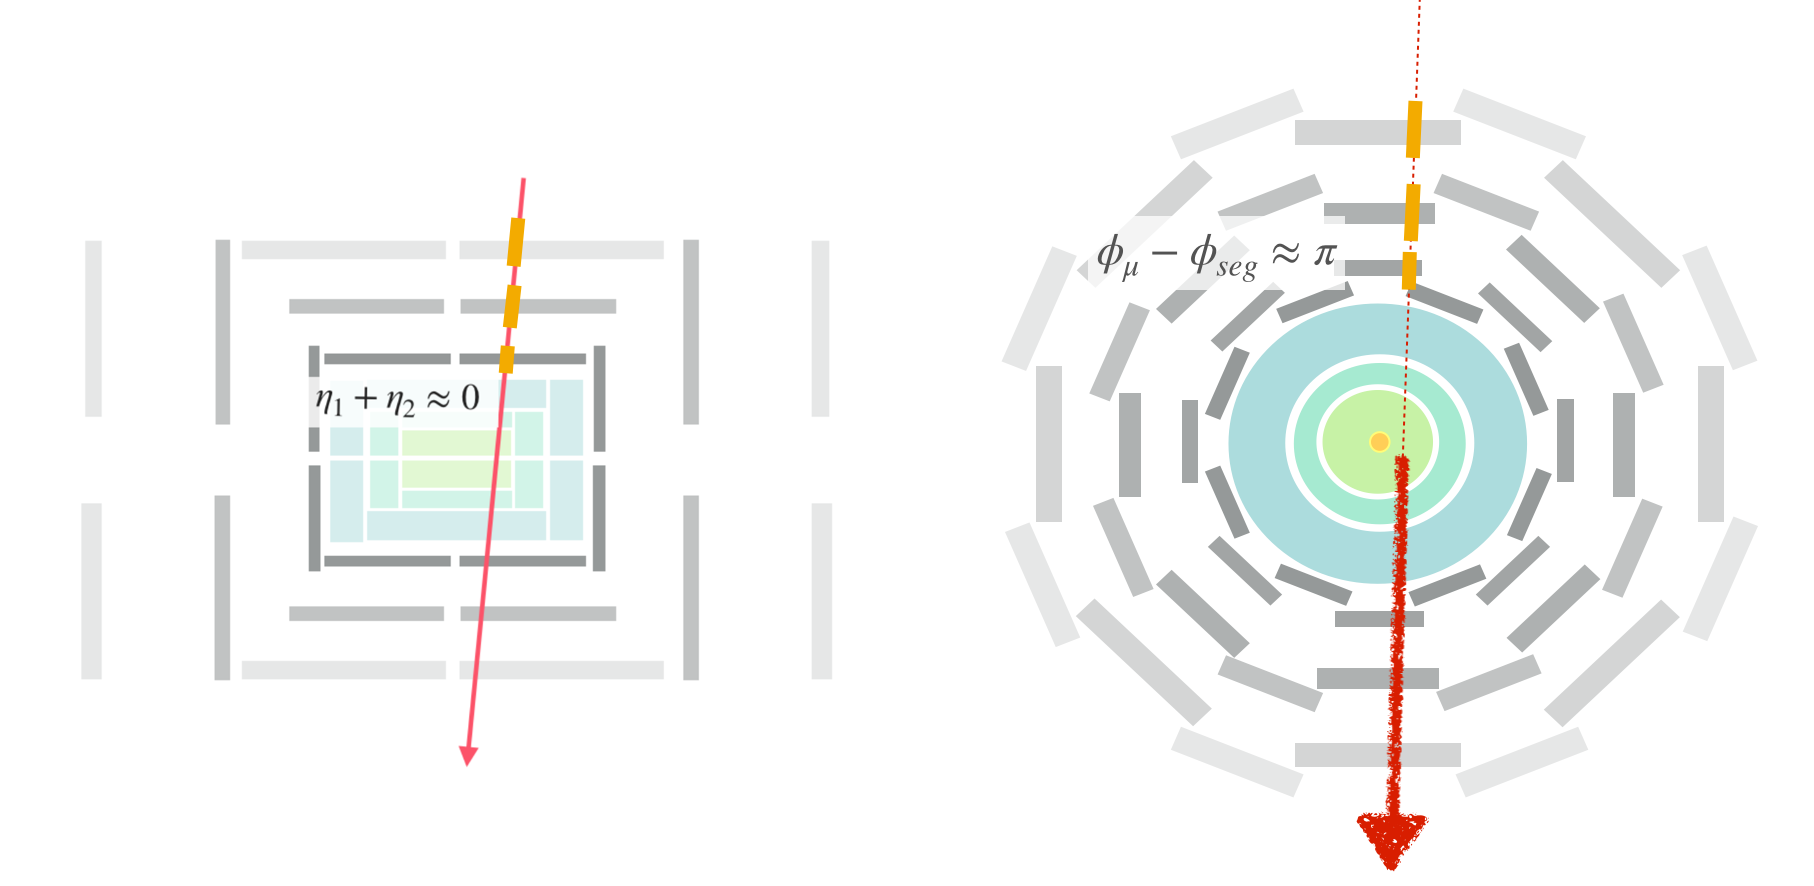
\includegraphics[width=.8\textwidth]{figures/cosmics/tag_sketch.png}
\caption{A sketch of a cosmic passing through the ATLAS detector, illustrating why the tag is designed the way that it is. This image is slightly adapted from Ref.~\cite{dvplusmu}}
\label{fig:tag_sketch}
\end{figure}

Since the \ac{MS} is so far from the \ac{PV}, the \z of individual MS segments is not measured and they are defined to point back to the origin. This creates a mismatch between the $\eta$ of the segment and the $\eta$ of the reconstructed muon in the determination of the cosmic tag. This is geometrically corrected for by re-calculating the $\Delta\eta$ between the segment and the muon in the cosmic veto calculation. A schematic of this correction is shown in \autoref{fig:cos_eta_recalculation}, its effect on the $\eta$ and \sigeta measurements of muons in data is shown in \autoref{fig:changeEta}, and its effect on the \dphicos-\sigeta distribution of cosmic and signal muons shown in \autoref{fig:cos_eta_phi}. This narrows the distribution of cosmic muons by an order of magnitude in \sigeta. This distribution is isotropic for signal muons, so this definition allows for high cosmic muon rejection with minimal signal rejection. 

\begin{figure}[!ht]
\centering
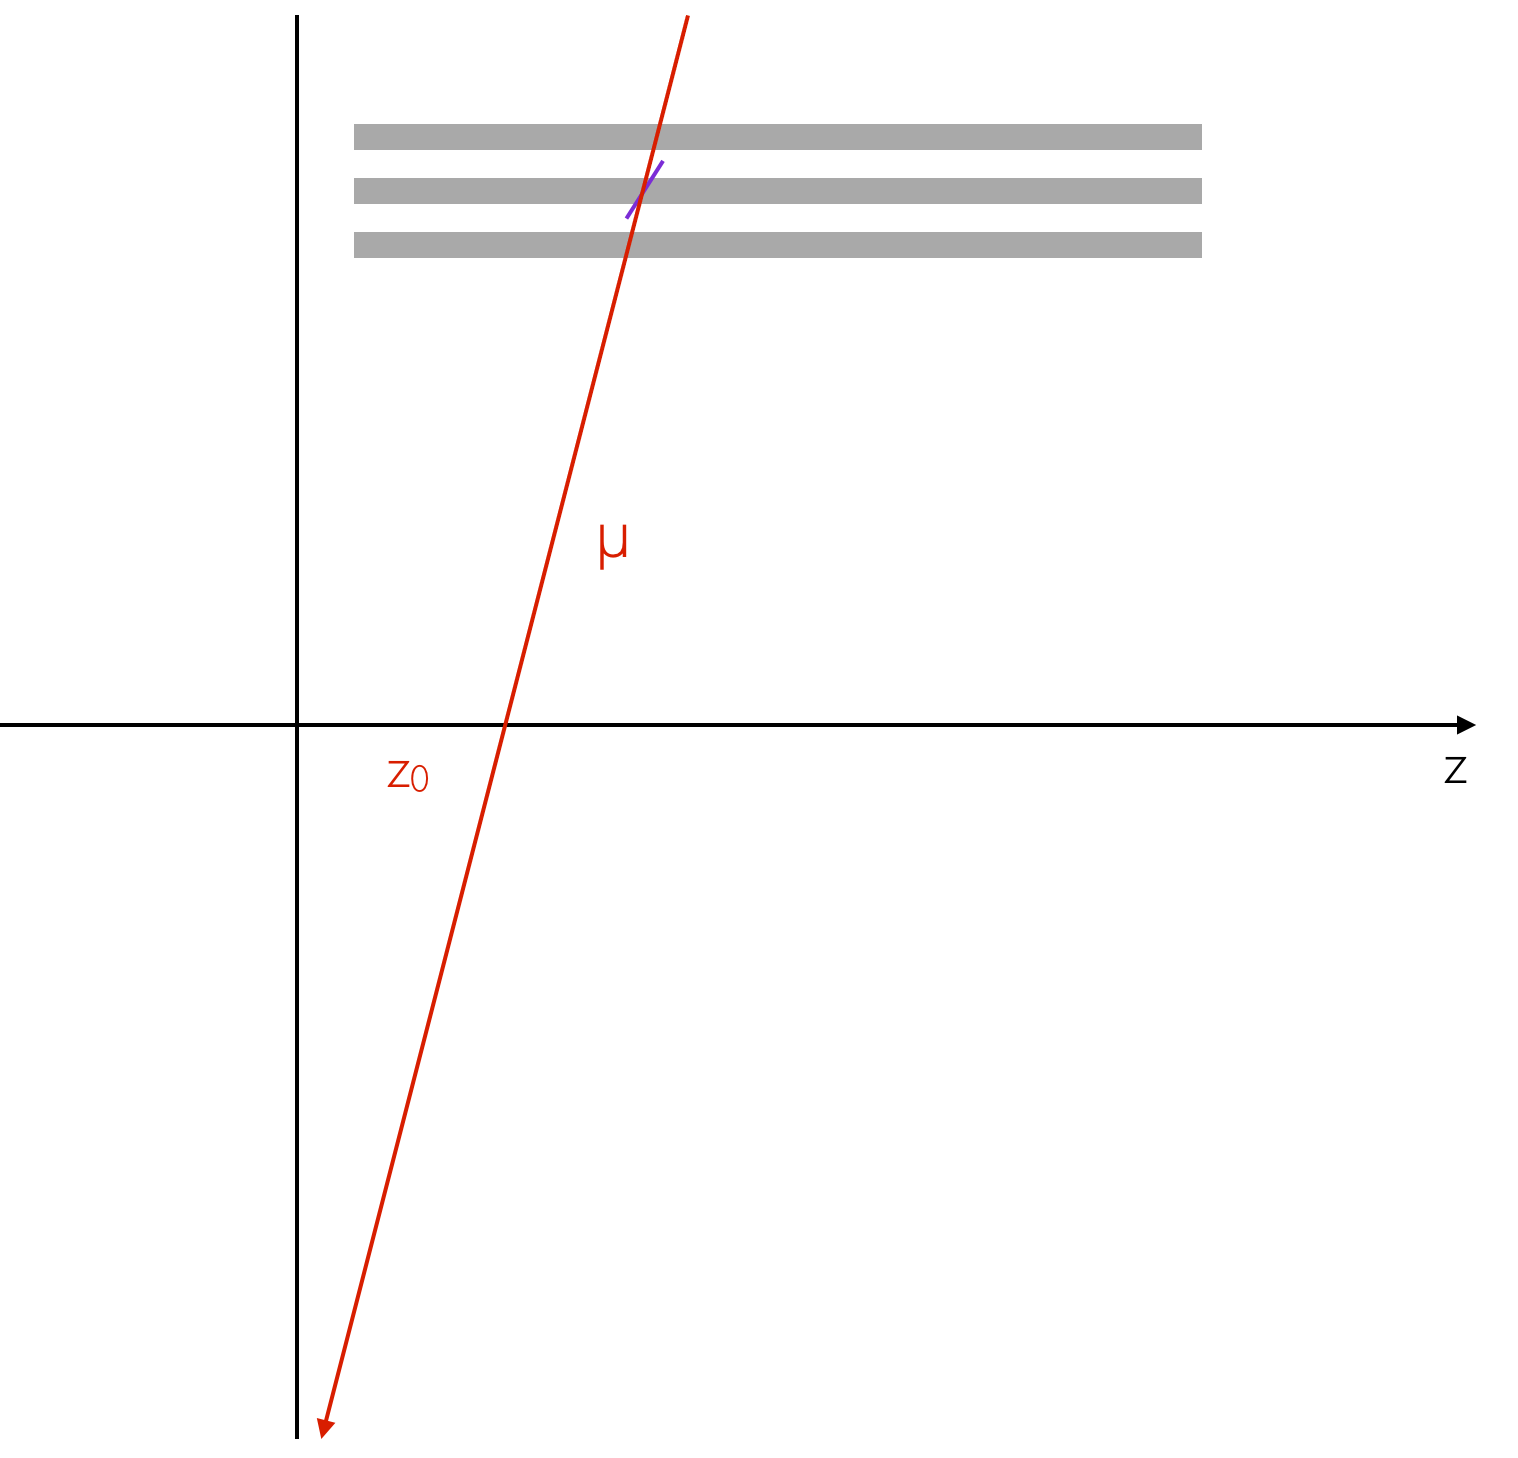
\includegraphics[height=4cm]{figures/cosmics/eta_correction_1.png}
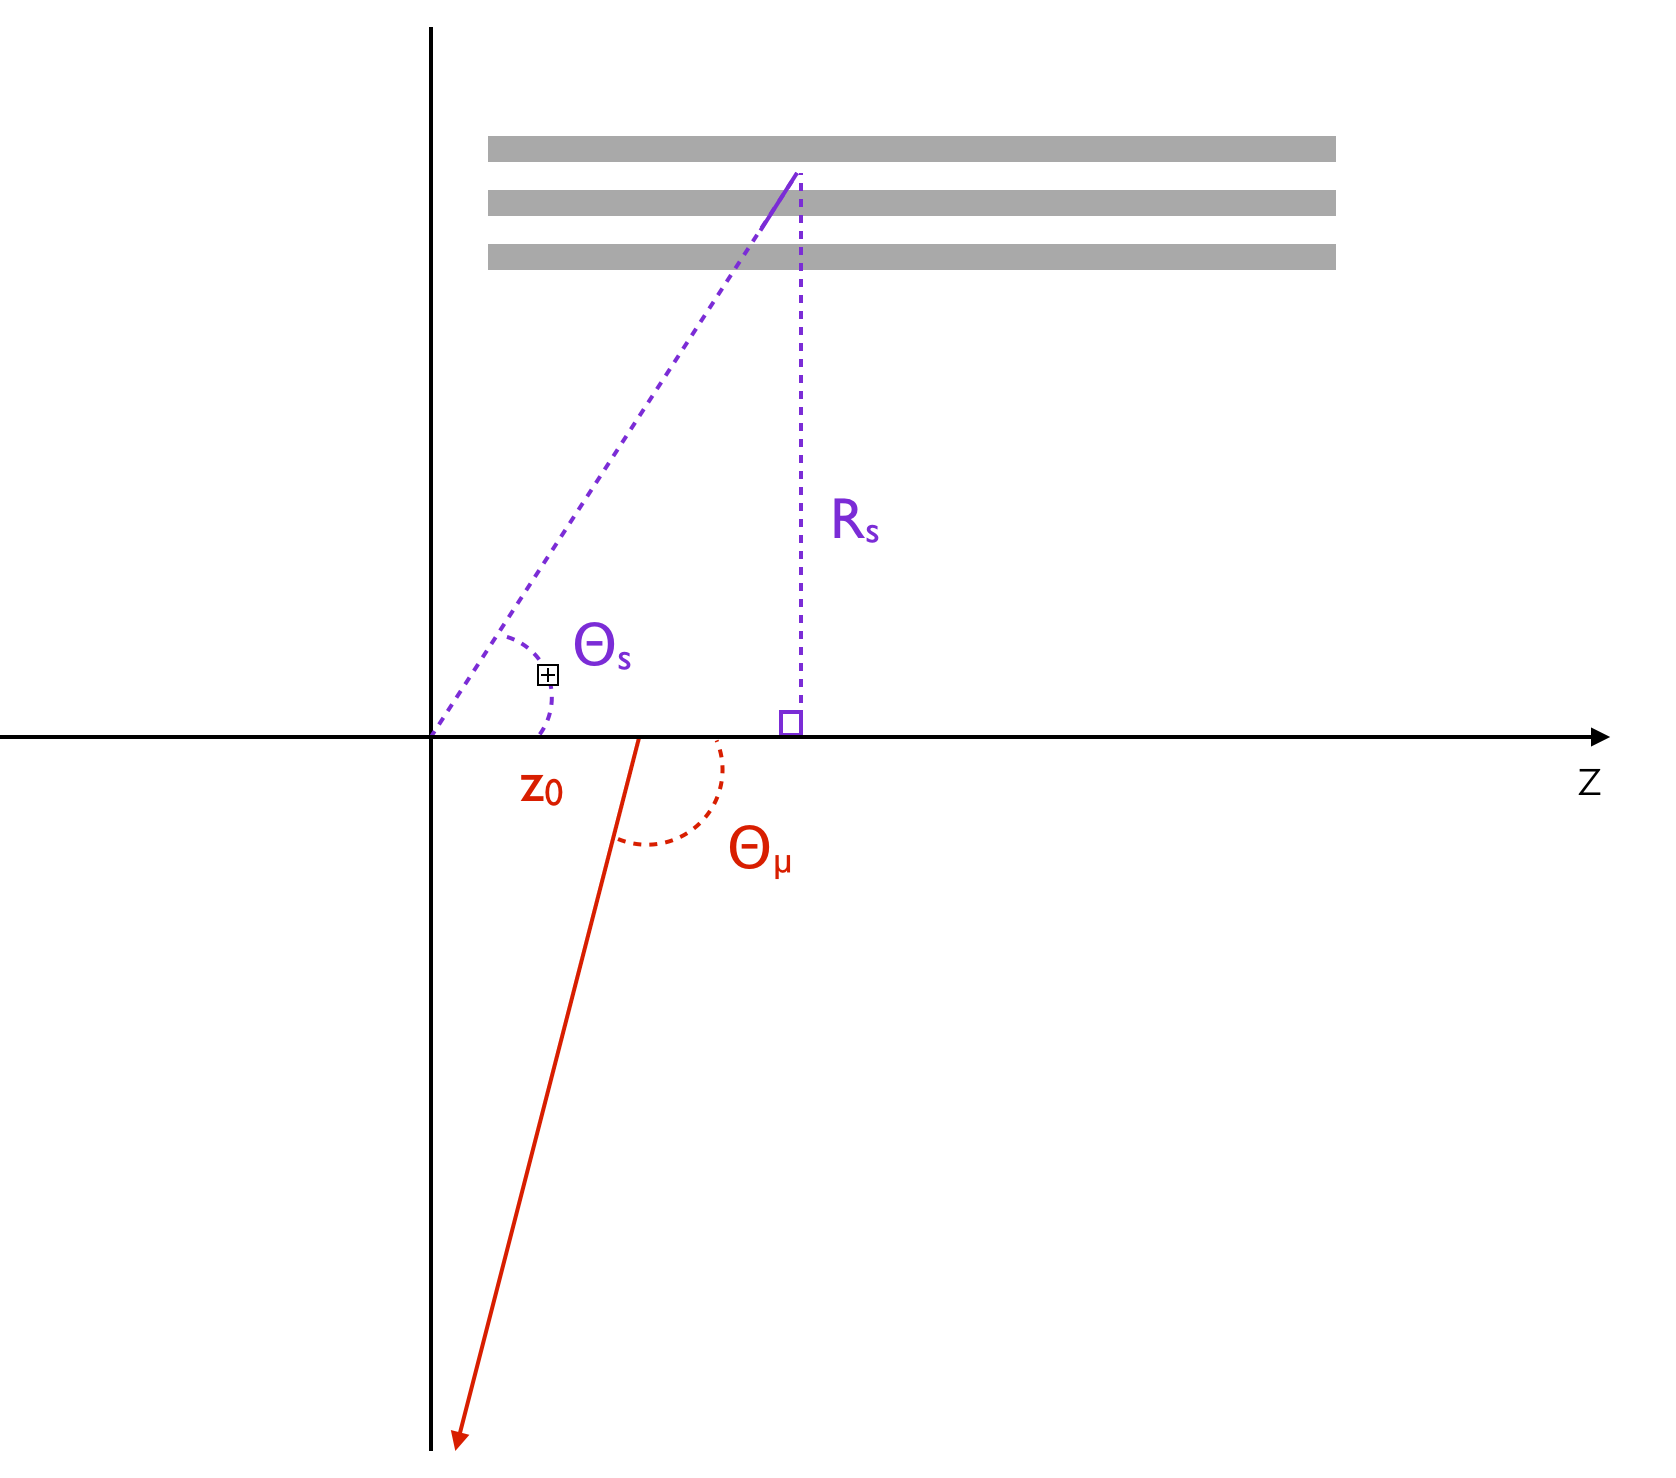
\includegraphics[height=4cm]{figures/cosmics/eta_correction_2.png}
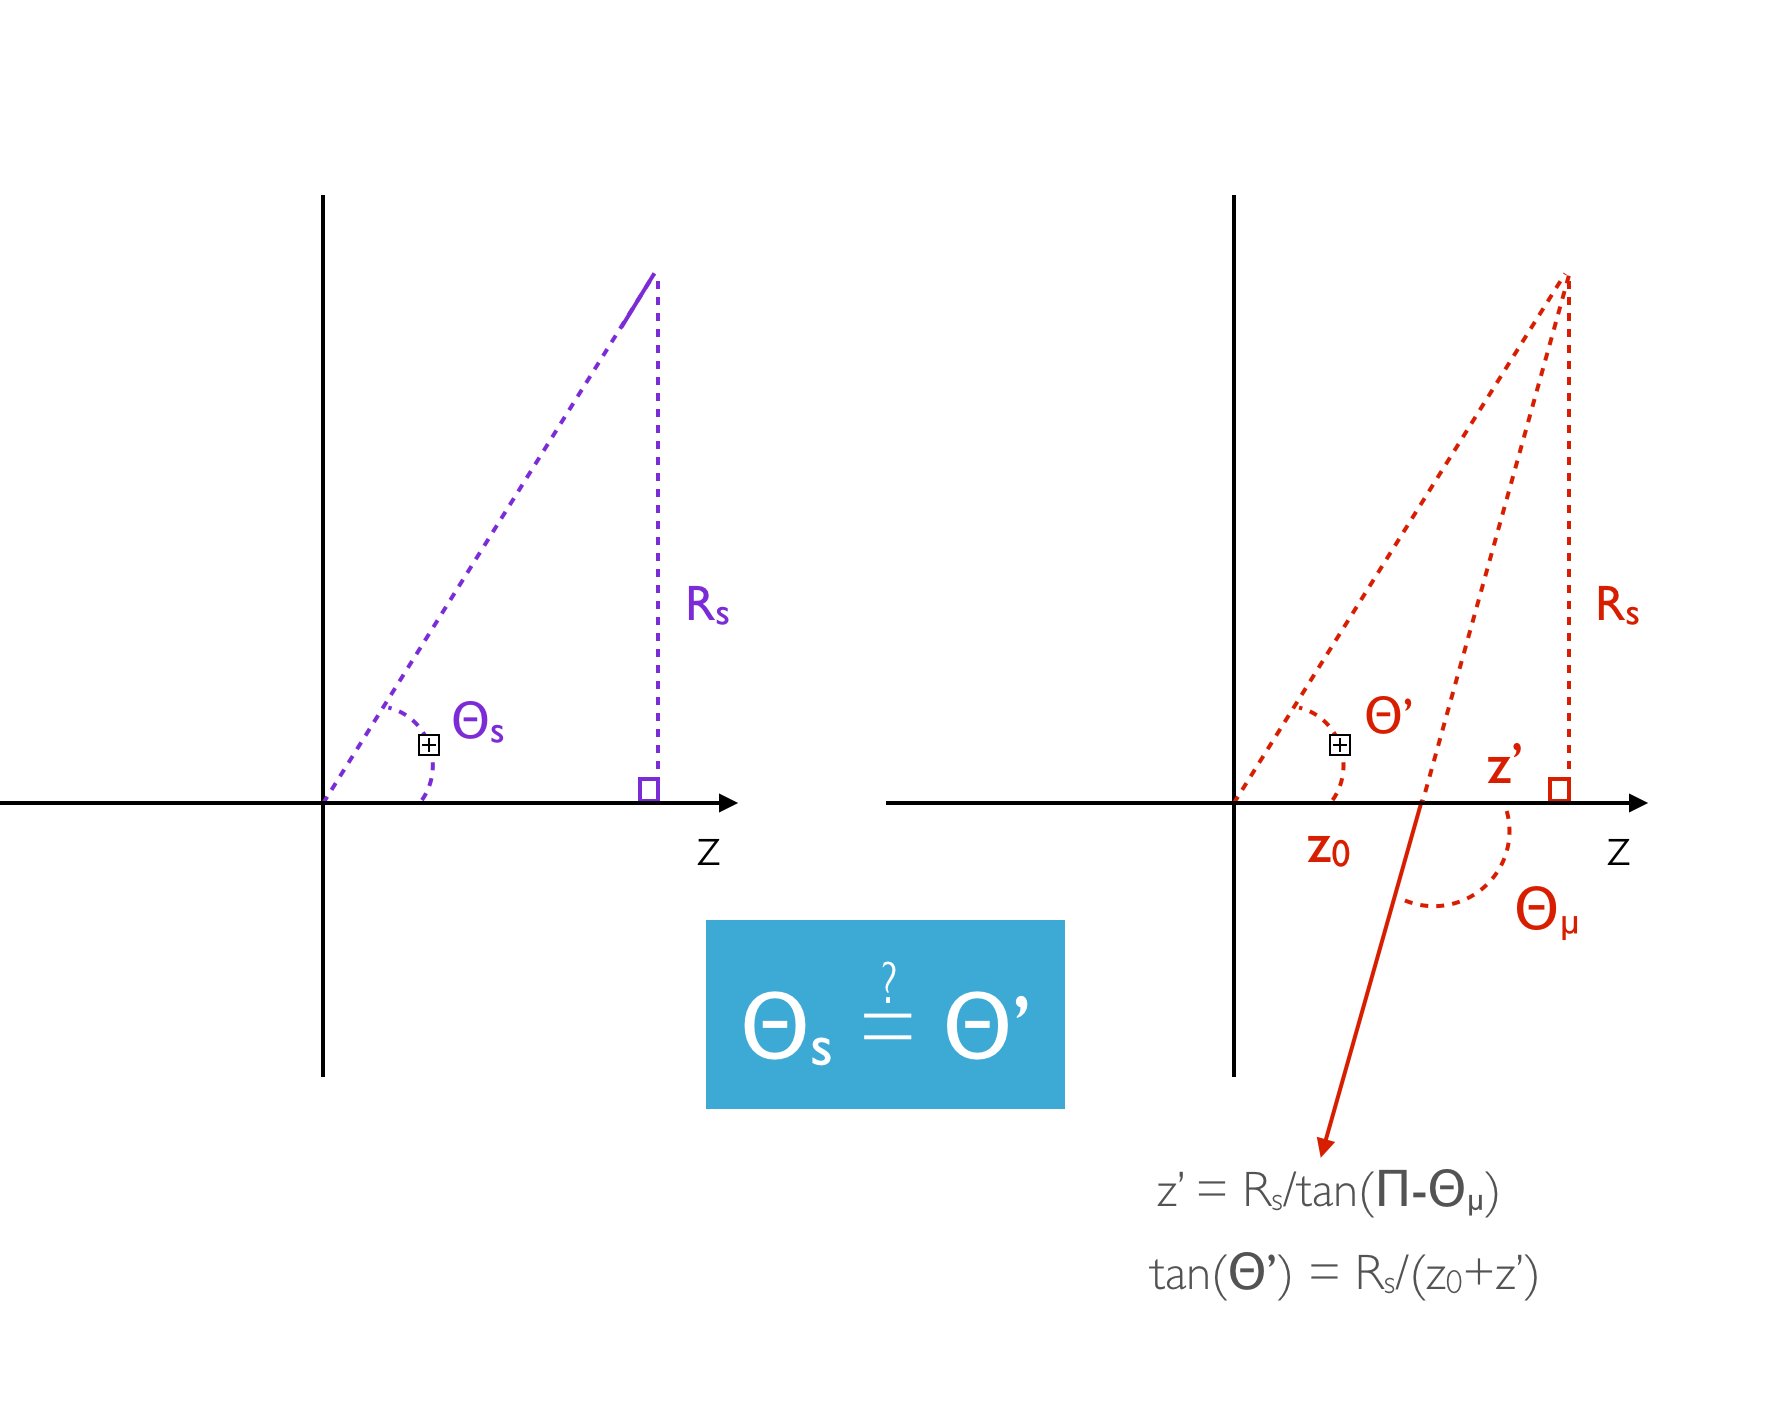
\includegraphics[height=5cm]{figures/cosmics/eta_correction_3.png}
\caption{This series of figures shows the problem of the $\eta$ recalculation. The MS segment should be measured as back to back in $\eta$ and $\phi$ with the muon, because it is really one high $p_{T}$ object moving through the whole detector. However, because the MS segments are reconstructed assuming they come from the origin, they will not actually be measured as back-to-back with the muon. The $\eta$ that would be measured by a segment back to back with the muon is calculated, and compared to the $\eta$ of all other segments in the event.}
\label{fig:cos_eta_recalculation}
\end{figure}

\begin{figure}[!ht]
\centering
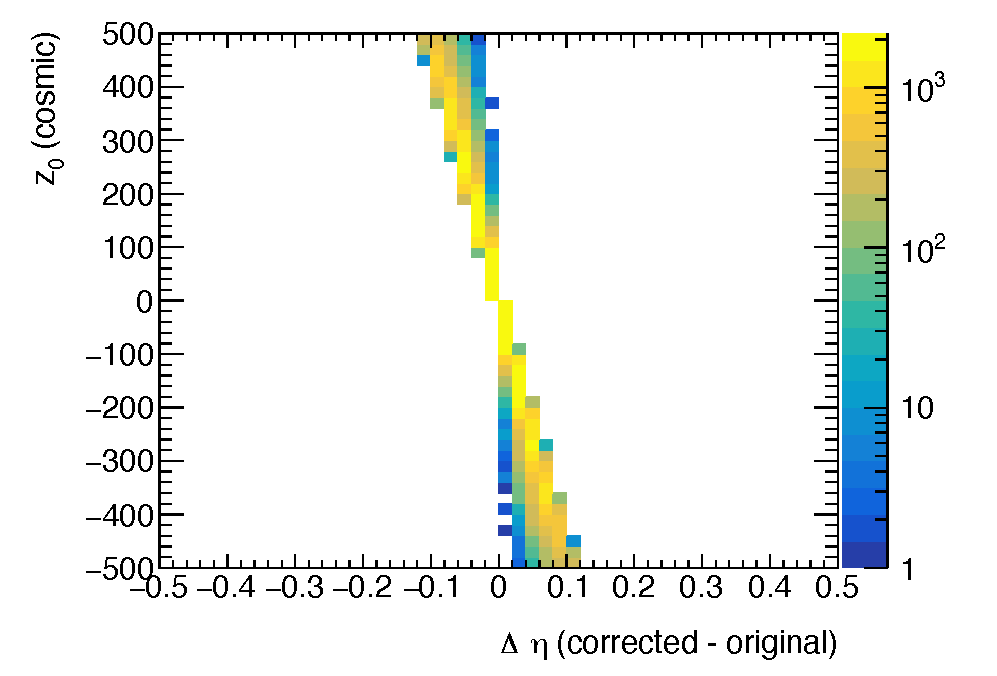
\includegraphics[width=.48\textwidth]{figures/cosmics/cosnotmv_z0_dEta_corr.pdf}
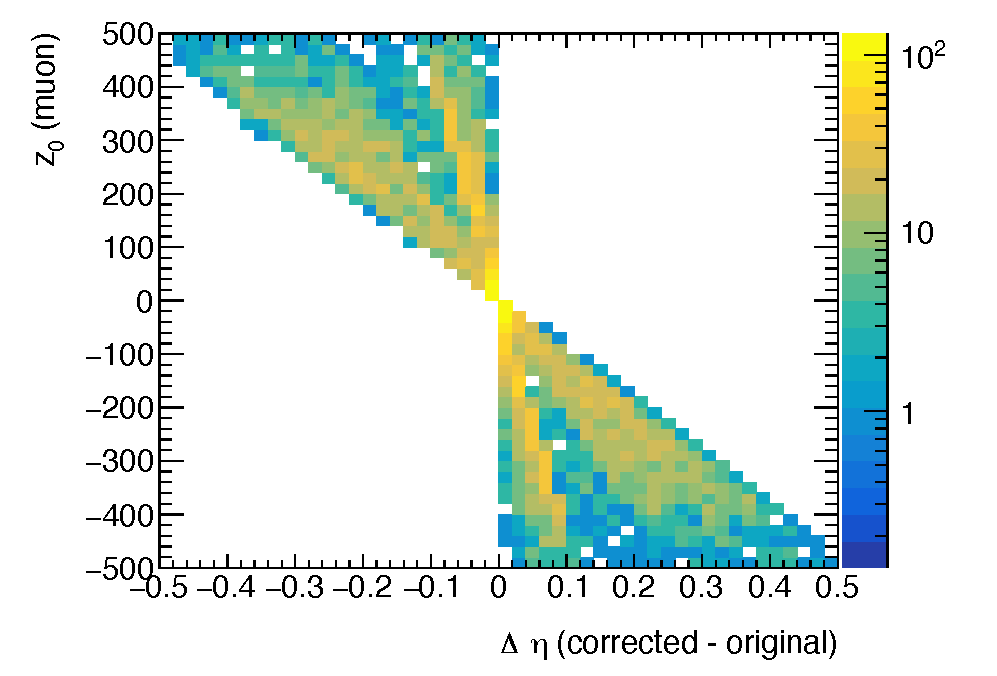
\includegraphics[width=.48\textwidth]{figures/cosmics/mvmu_z0_dEta_corr.pdf}
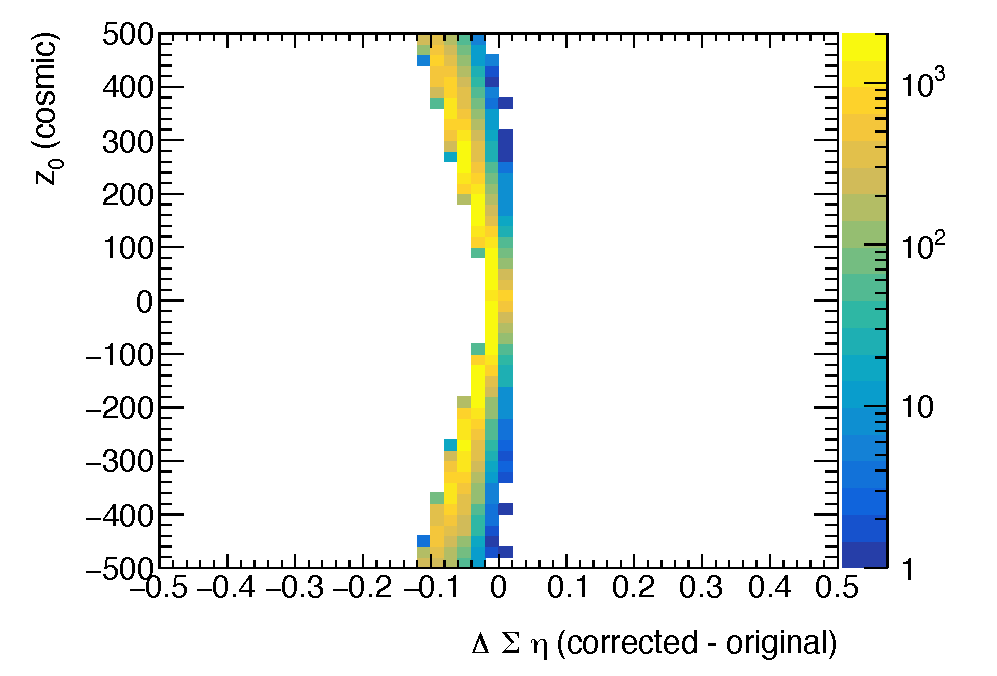
\includegraphics[width=.48\textwidth]{figures/cosmics/cosnotmv_z0_dSeta_corr.pdf}
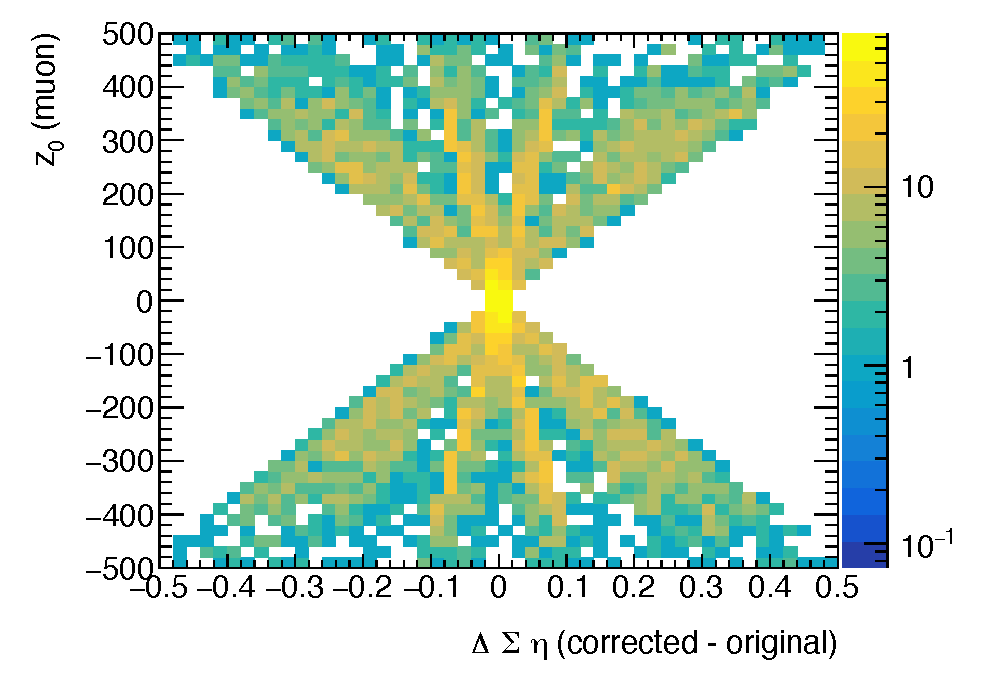
\includegraphics[width=.48\textwidth]{figures/cosmics/mvmu_z0_dSeta_corr.pdf}
\caption{Change to the $\eta$ measurement (top) and \sigeta measurement (bottom) due to the $z_{0}$ correction. These plots compare muons tagged with due to the presences of a segment in the \dphicos-\sigeta window (left) to those untagged or tagged with the detector coverage veto (right). The behavior shows isotropic effect for the muons which are not tagged via the algorithm that uses this correction, while the \sigeta distribution of cosmic muon always decreases due to the correction.}
\label{fig:changeEta}
\end{figure}


\begin{figure}[!ht]
\centering
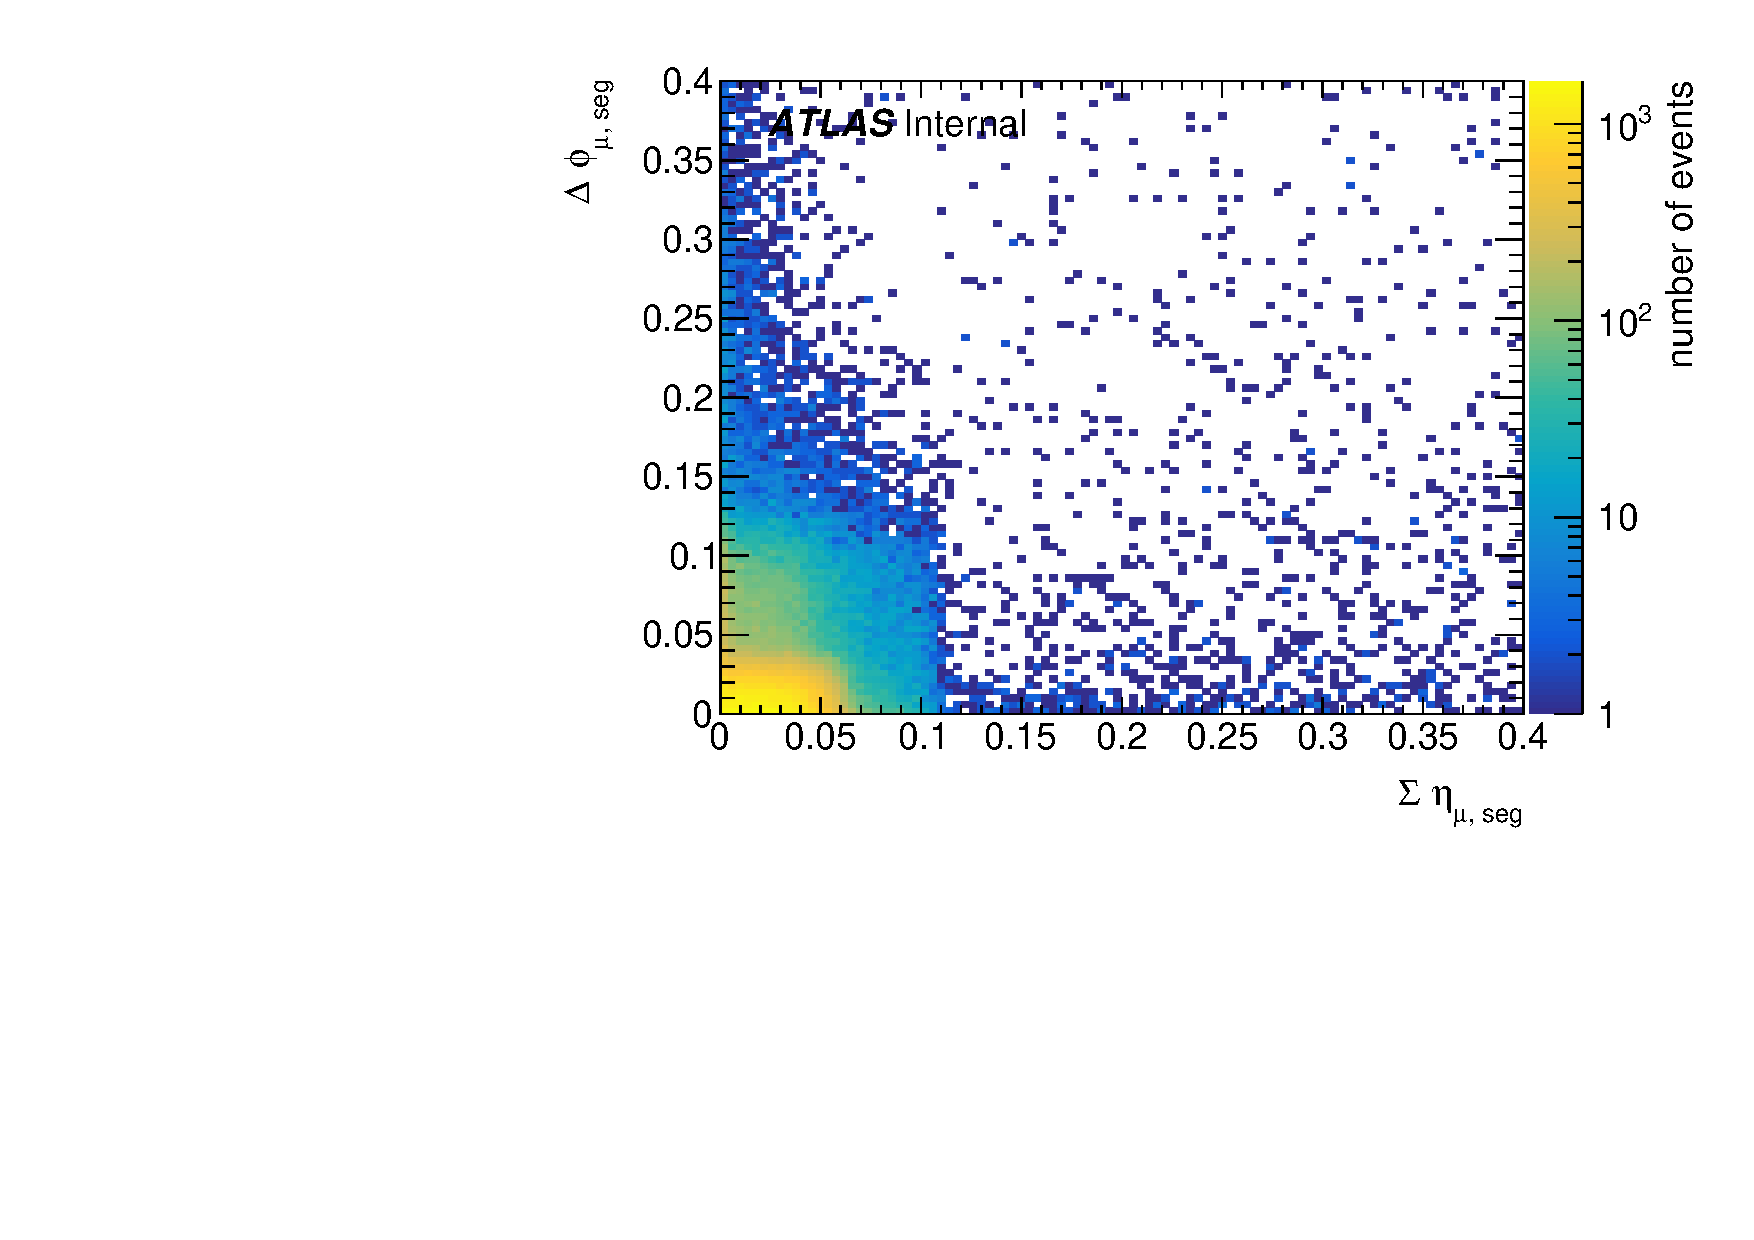
\includegraphics[width=.48\textwidth]{figures/cosmics/v4_widetag_2_sumEta_dPhi_min.pdf}
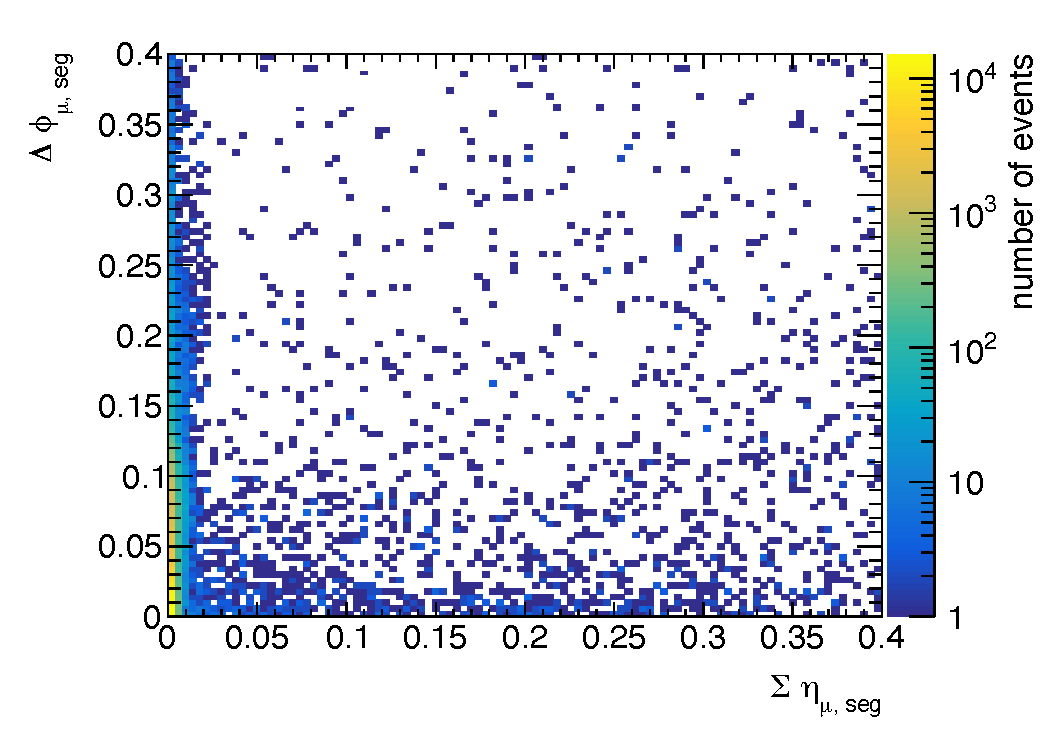
\includegraphics[width=.48\textwidth]{figures/cosmics/v4_widetag_2_sumEta_dPhi_min_corr.pdf}
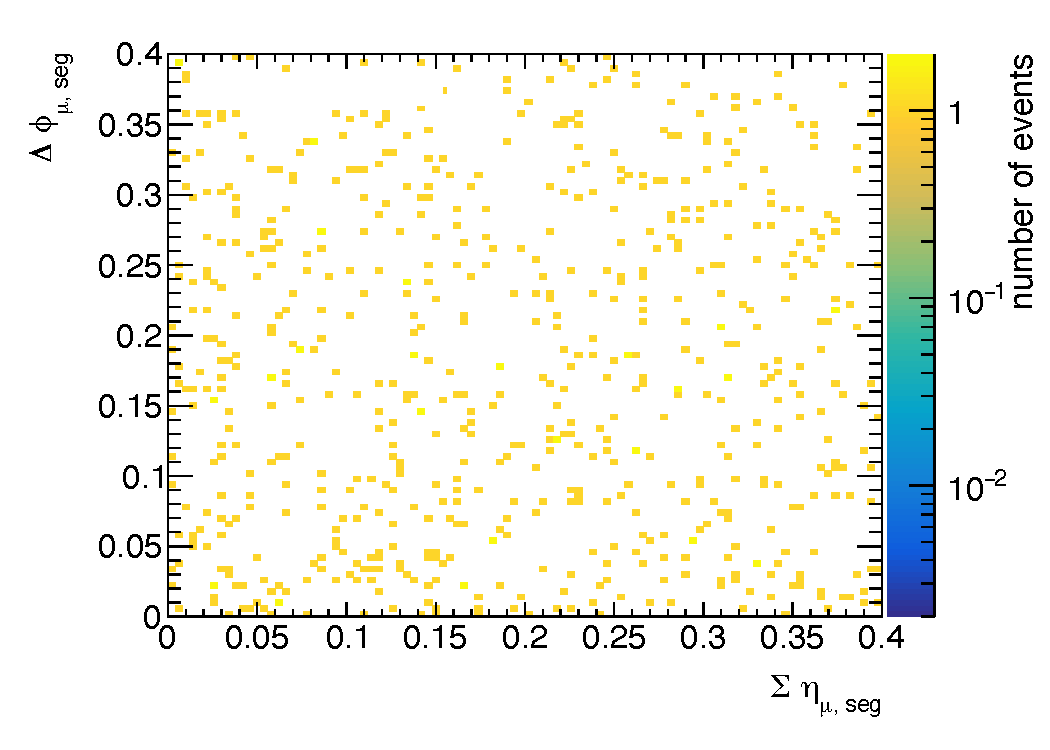
\includegraphics[width=.48\textwidth]{figures/cosmics/300_slep_2_sumEta_dPhi_min.pdf}
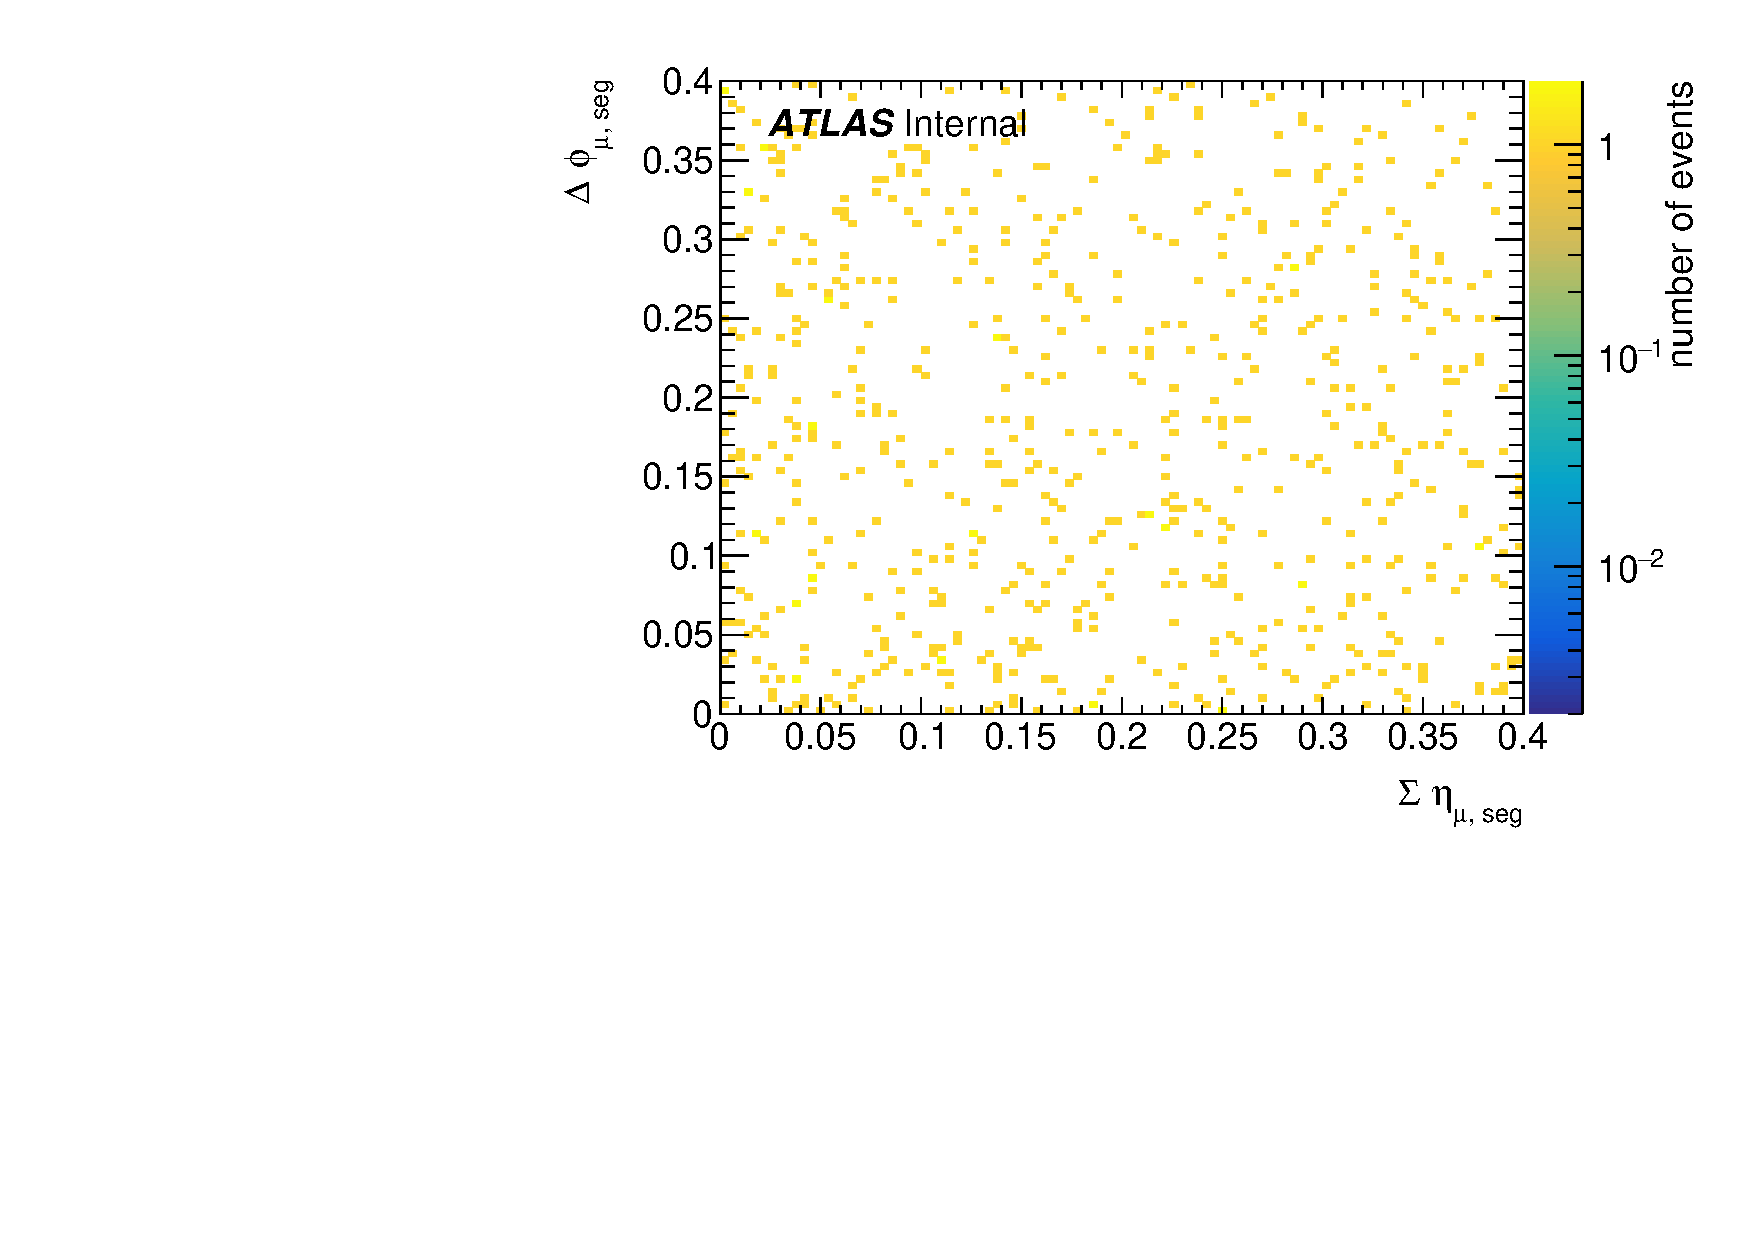
\includegraphics[width=.48\textwidth]{figures/cosmics/300_slep_2_sumEta_dPhi_min_corr.pdf}
\caption{The $\Sigma\eta - \Delta\phi$ distribution is shown before (left) and after (right) the $\eta$ recalculation. The top row shows the distributions in VR-$\mu$ and bottom row 300 GeV \slep signal samples in our full range of lifetimes. Using this cosmic tag, a very tight cut can be made on cosmic muons without losing signal efficiency.}
\label{fig:cos_eta_phi}
\end{figure}


The distribution the $\dphicos-\sigeta$ distribution is much narrower in \sigeta than in \dphicos. This is because the \ac{MS} measures $\eta$ with an extremely high precision in the \acp{MDT} ($\mathcal{O}(10~\um)$), since it is the bending direction of the toroid and thus gives the momentum measurement, while the $\phi$ is measured by the \acp{RPC} with an order of magnitude less precision ($\mathcal{O}(10~\text{mm})$). A high precision $\phi$ measurement of the combined muon comes from the \ac{ID}, but the cosmic tag must contend with these resolution limitations to find a muon segment.

Additionally, there are gaps in the \ac{MS} to allow for detector access, so a muon is conservatively tagged as a cosmic if it is back to back with this gap in detector coverage, as it could not be tagged as a cosmic using the geometric algorithm. A map of the material of the \ac{MS} is used to veto cosmic muons using this \emph{detector coverage veto}. \autoref{fig:cos_material_veto} shows the impact of each step on the muon distribution in VR-$\mu$, which is dominated by muons from cosmic rays.


\begin{figure}[!ht]
\centering
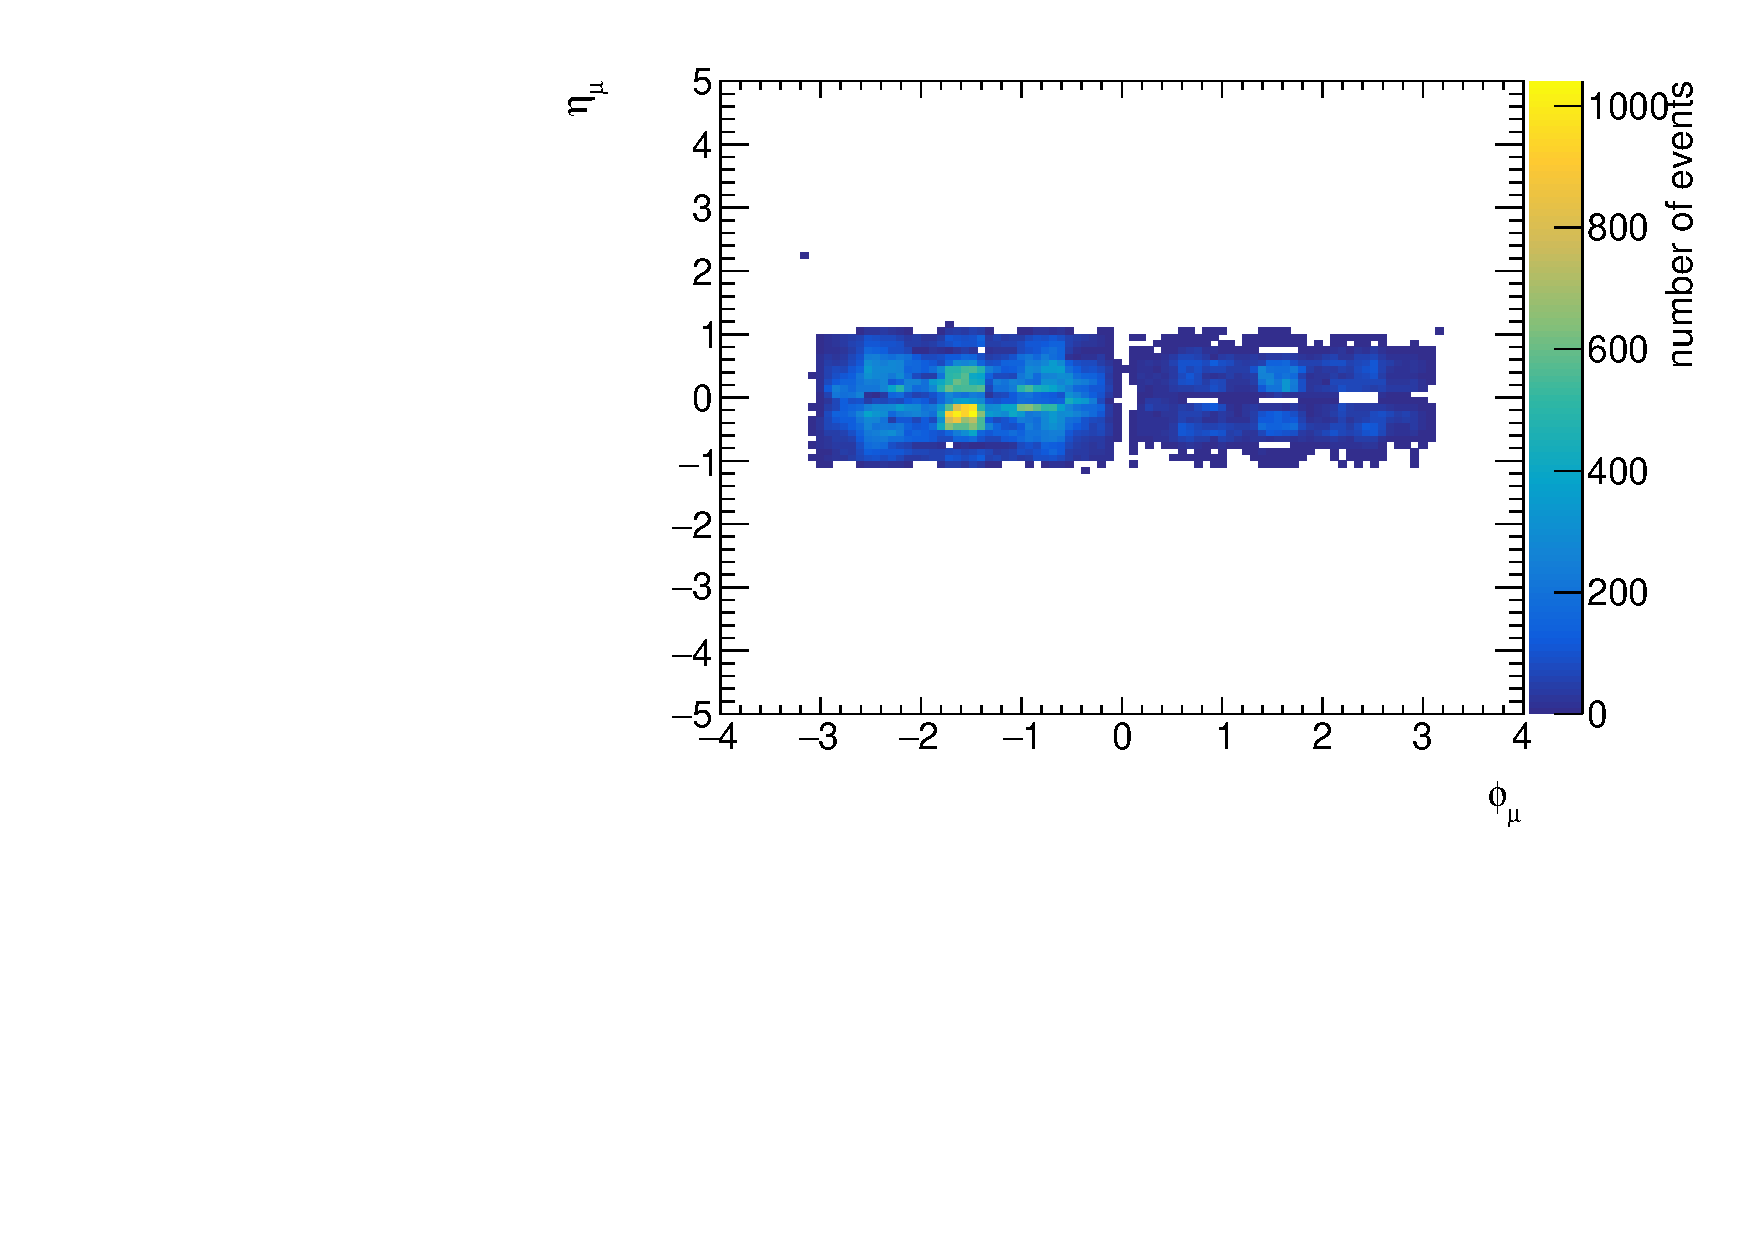
\includegraphics[width=.48\textwidth]{figures/cosmics/v4_widetag_2_eta_phi_baseline.pdf}
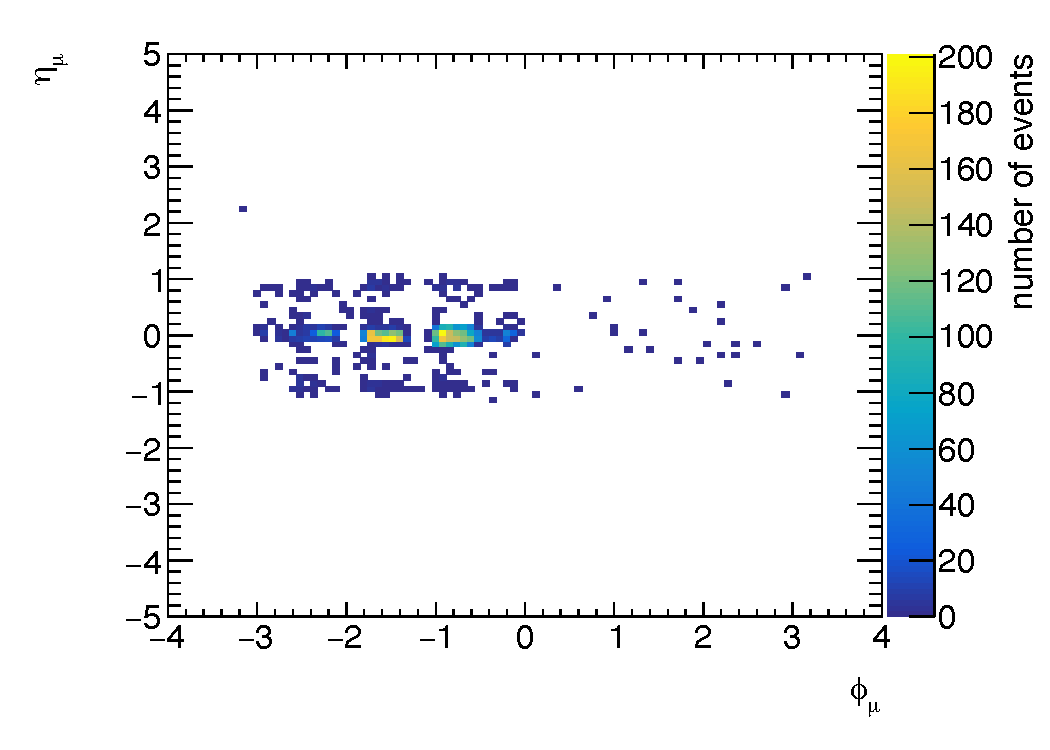
\includegraphics[width=.48\textwidth]{figures/cosmics/v4_widetag_2_eta_phi_costag.pdf}
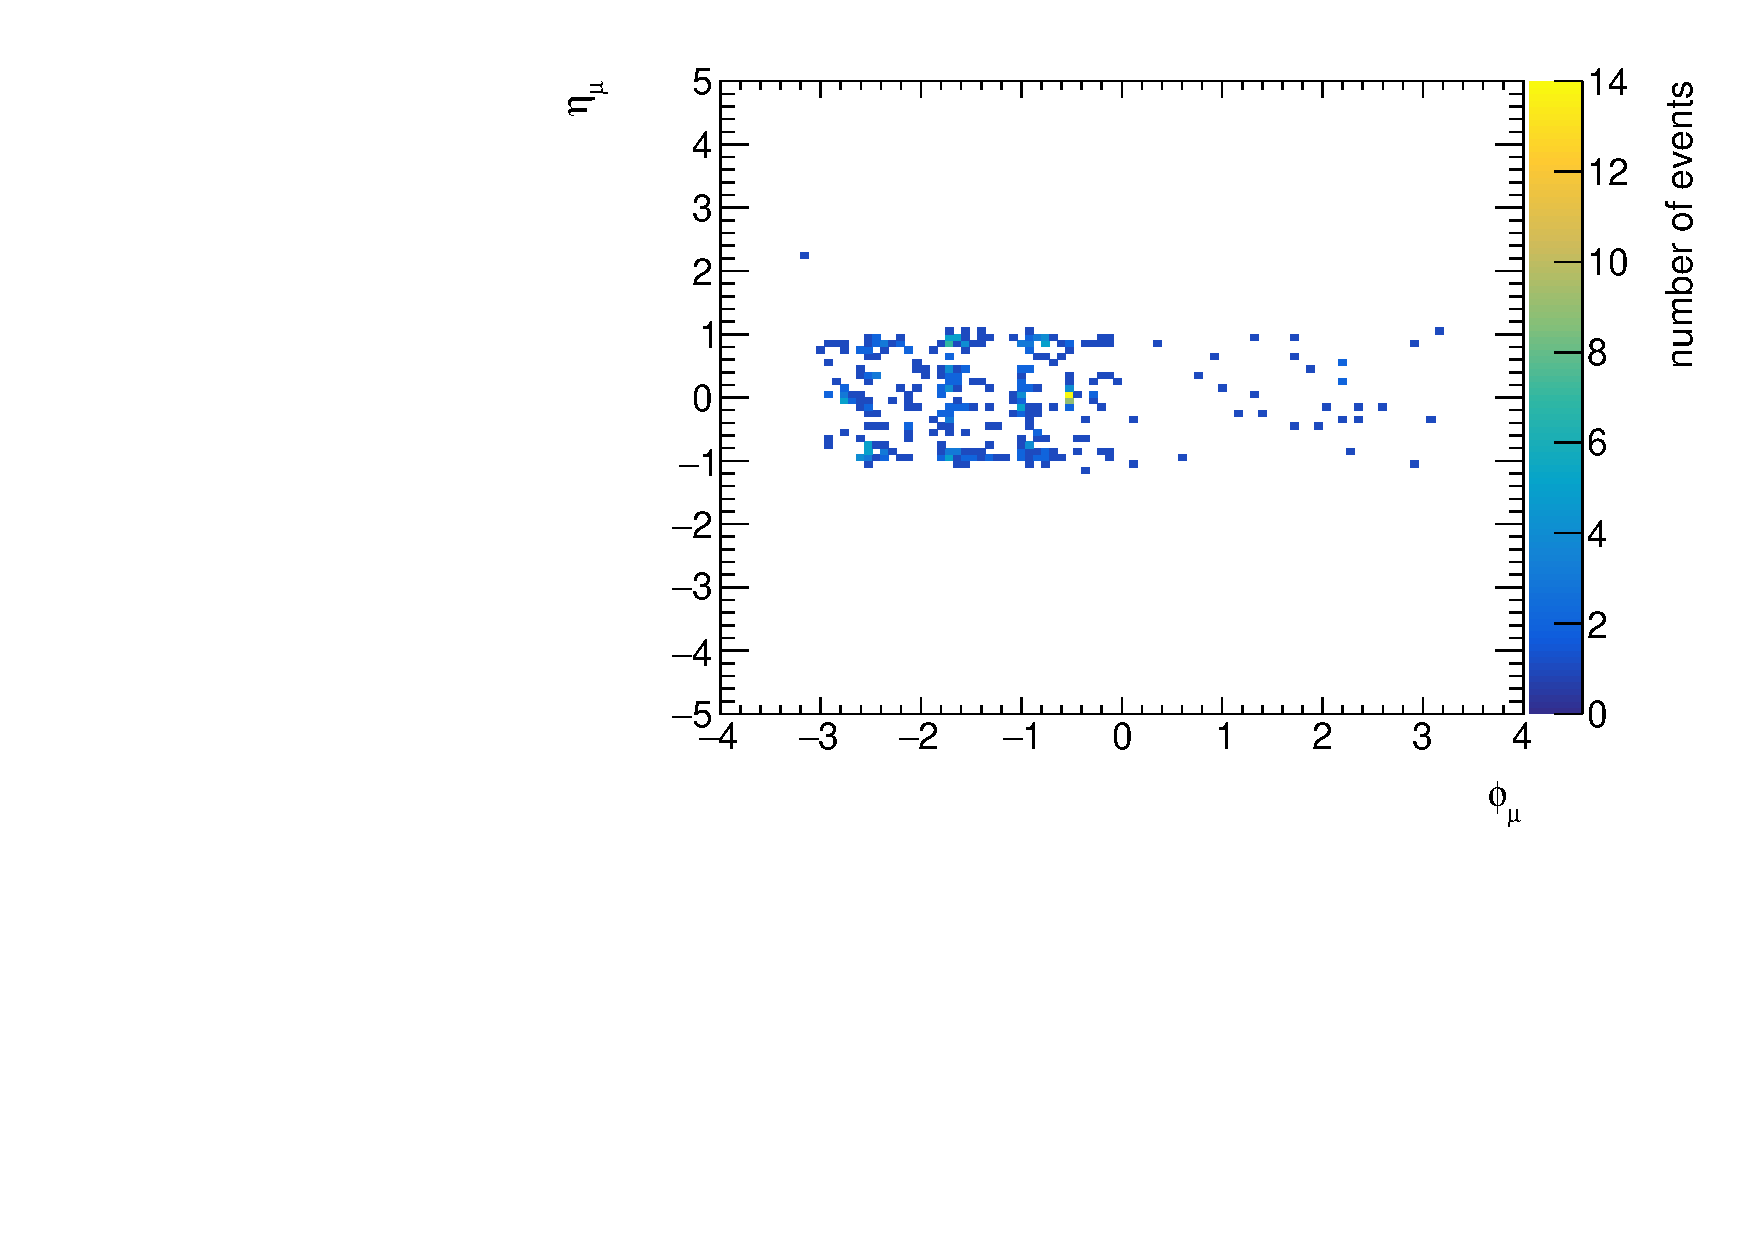
\includegraphics[width=.48\textwidth]{figures/cosmics/v4_widetag_2_eta_phi_costag_mv.pdf}
\caption{The $\eta-\phi$ distribution of muons in VR-$\mu$ are shown after baseline cuts (top left), the cosmic veto (top right), then the detector coverage veto (bottom).}
\label{fig:cos_material_veto}
\end{figure}

For this analysis, two different definitions of a ``cosmic muon'' are used. The \emph{nominal tag} is used to veto events in the \ac{SR}. If any baseline muon is tagged by the nominal cosmic tag, the entire event is vetoed. A second \emph{narrow tag} is used during the validation of the estimate of background from cosmic muons. Both tags require muons to pass the detector coverage veto. \autoref{tab:costag_values} describes the values used for the various cosmic tags used and \autoref{fig:cos_tag} shows the cuts used in the \dphicos-\sigeta distribution. 

\begin{figure}[!ht]
\centering
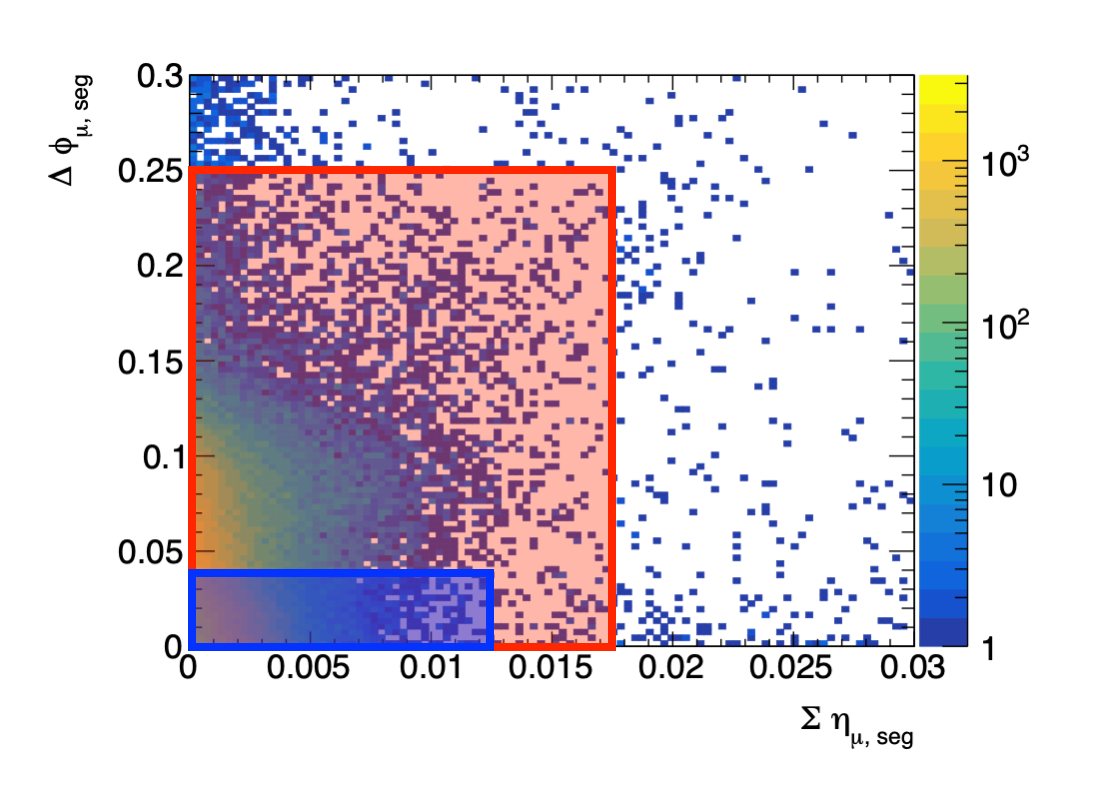
\includegraphics[width=.48\textwidth]{figures/cosmics/cosmic_tag.png}
\caption{The $\Sigma\eta_{\mu,\textrm{seg}} - \Delta\phi_{\mu,\textrm{seg}}$ distribution of signal quality muons in VR-$\mu$. The red line and shadow shows the bounds of the full cosmic tag, while the blue line and shadow shows the boundary of the narrow cosmic tag. Everything inside the respective boxes is tagged as a cosmic. The intermediate tag defines the region included in the full tag, but not included in the narrow tag.}
\label{fig:cos_tag}
\end{figure}

\begin{table}
\centering
\begin{tabular}{lcccc}
Tag & $\Delta \phi (\mu, \textrm{seg})$ & $\Sigma \eta (\mu, \textrm{seg})$ & Pass Coverage  & Rejection \\
 &                                         &                                &    Acceptance & Efficiency \\
\hline
Full   & $<0.25$   & $ <0.018 $   & True & 99.5\% \\
Narrow & $<0.02$   & $ <0.013$    & True & 59\% \\
\hline
\end{tabular}
\caption{Cuts applied in full and narrow cosmic tags. The narrow is contained in the full tag. An intermediate tag is defined as the region between the full and narrow tags, that is, tagged by the full but not the narrow tag.}
\label{tab:costag_values}
\end{table}

The cosmic tagging efficiency is determined by fitting distributions in VR-$\mu$. A template of the \tavg of cosmic tagged muons and prompt (collision) muons is taken from data shown on the left of \autoref{fig:d0_t0avg}. Any correlation between \tavg and \dz can not be observed within detector resolutions, so the prompt sample of muons is taken to represent the signal muons that would result from collisions.

These are used to determine the fraction of cosmic muons in VR-$\mu$ before and after the cosmic tagged muons are removed from VR-$\mu$ (left of \autoref{fig:d0_t0avg}). From the fraction of cosmic muons estimated from the template fitting, the fraction of muons removed by the cosmic tag can be measured. The nominal tag removes 99.5\% of cosmic muons and the narrow tag removes 59\% of cosmic muons. The nominal tag removes 8\% of collision muons, primarily from the detector coverage veto. \autoref{fig:cos_eff} compares the kinematic distributions and cosmic-tagging efficiency between VR-$\mu$ and signal \ac{MC}. 

\begin{figure}[!ht]
  \centering
  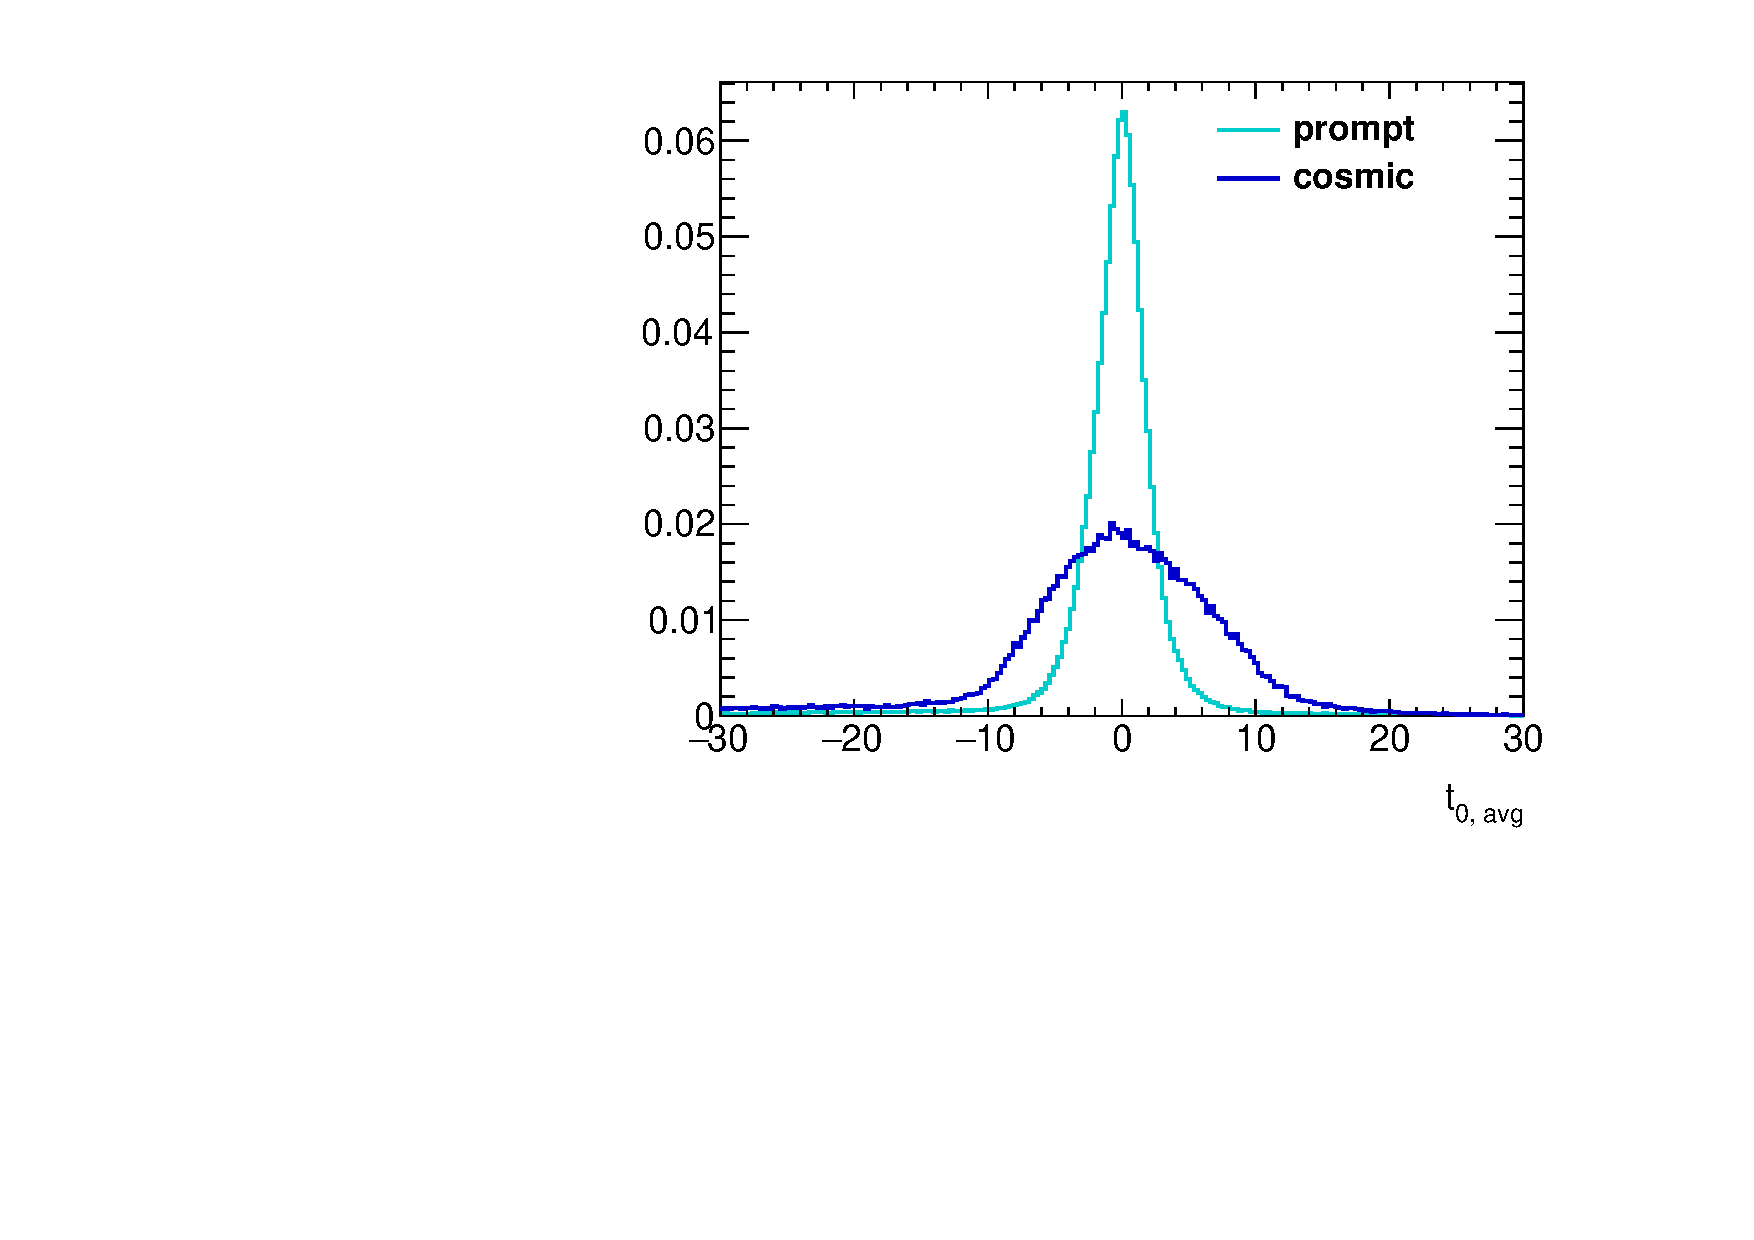
\includegraphics[width=0.38\textwidth]{figures/cosmics/t0_avg_template_comp.pdf}
  \includegraphics[width=0.38\textwidth]{figures/cosmics/t0_avg_prepost_comp.pdf}
  \caption{\tavg of cosmic and prompt muons used as templates to the fit (left) and VR-$\mu$ dataset before and after removal of cosmic tagged muons on which the fit was performed.}
  \label{fig:d0_t0avg}
\end{figure}


\begin{figure}[!ht]
  \centering
  \begin{subfigure}[b]{0.4\textwidth}
 	\includegraphics[width=\textwidth]{figures/cosmics/wider_tag_ratio_pt.pdf}
  	\caption{VR-$\mu$ data with respect to \pt}
  \end{subfigure}
  \begin{subfigure}[b]{0.4\textwidth}
 	\includegraphics[width=\textwidth]{figures/cosmics/mc_300_ratio_pt.pdf}
  	\caption{Signal \ac{MC} with respect to \pt}
  \end{subfigure}

  \begin{subfigure}[b]{0.4\textwidth}
  	\includegraphics[width=\textwidth]{figures/cosmics/wider_tag_ratio_d0.pdf}
  	\caption{VR-$\mu$ data with respect to \dz}
  \end{subfigure}
  \begin{subfigure}[b]{0.4\textwidth}
  	\includegraphics[width=\textwidth]{figures/cosmics/mc_300_ratio_d0.pdf}
  	\caption{Signal \ac{MC} with respect to \dz}
  \end{subfigure}

  \begin{subfigure}[b]{0.4\textwidth}
  	\includegraphics[width=\textwidth]{figures/cosmics/wider_tag_ratio_z0.pdf}
  	\caption{VR-$\mu$ data with respect to \z}
  \end{subfigure}
  \begin{subfigure}[b]{0.4\textwidth}
  	\includegraphics[width=\textwidth]{figures/cosmics/mc_300_ratio_z0.pdf}
  	\caption{Signal \ac{MC} with respect to \z}
  \end{subfigure}
  \caption{Cosmic tagging efficiency with respect to kinematic variables in VR-$\mu$ data and signal \ac{MC}}
\end{figure}
\begin{figure}[!ht]
  \ContinuedFloat
  \centering
  \begin{subfigure}[b]{0.4\textwidth}
  	\includegraphics[width=\textwidth]{figures/cosmics/wider_tag_ratio_phi.pdf}
  	\caption{VR-$\mu$ data with respect to $\phi$}
  \end{subfigure}
  \begin{subfigure}[b]{0.4\textwidth}
 	\includegraphics[width=\textwidth]{figures/cosmics/mc_300_ratio_phi.pdf}
  	\caption{Signal \ac{MC} with respect to $\phi$}
  \end{subfigure}

 \begin{subfigure}[b]{0.4\textwidth}
  	\includegraphics[width=\textwidth]{figures/cosmics/wider_tag_ratio_eta.pdf}
  	\caption{VR-$\mu$ data with respect to $\eta$}
  \end{subfigure}
  \begin{subfigure}[b]{0.4\textwidth}
  	\includegraphics[width=\textwidth]{figures/cosmics/mc_300_ratio_eta.pdf}
  	\caption{Signal \ac{MC} with respect to $\eta$}
  \end{subfigure}
    \caption{Cosmic tagging efficiency with respect to kinematic variables in VR-$\mu$ data and signal \ac{MC}}
  \label{fig:cos_eff}
\end{figure}



%\begin{sidewaysfigure}[h]
%  \centering
%  \begin{subfigure}[b]{\textwidth}
%  	\centering
%  	\includegraphics[width=.18\textwidth]{figures/cosmics/wider_tag_ratio_pt.pdf}
%  	\includegraphics[width=.18\textwidth]{figures/cosmics/wider_tag_ratio_d0.pdf}
% 	\includegraphics[width=.18\textwidth]{figures/cosmics/wider_tag_ratio_z0.pdf}
% 	\includegraphics[width=.18\textwidth]{figures/cosmics/wider_tag_ratio_phi.pdf}
% 	\includegraphics[width=.18\textwidth]{figures/cosmics/wider_tag_ratio_eta.pdf}
% 	\caption{Cosmic tagging efficiency in VR-$\mu$ data}
%  \end{subfigure}

%  \begin{subfigure}[b]{\textwidth}
%  	\centering
%  	\includegraphics[width=.18\textwidth]{figures/cosmics/mc_300_ratio_pt.pdf}
%  	\includegraphics[width=.18\textwidth]{figures/cosmics/mc_300_ratio_d0.pdf}
%  	\includegraphics[width=.18\textwidth]{figures/cosmics/mc_300_ratio_z0.pdf}
%  	\includegraphics[width=.18\textwidth]{figures/cosmics/mc_300_ratio_phi.pdf}
%  	\includegraphics[width=.18\textwidth]{figures/cosmics/mc_300_ratio_eta.pdf}
%  	\caption{Cosmic tagging efficiency in signal \ac{MC}.}
%  \end{subfigure}
%    \caption{Cosmic tagging efficiency with respect to \pt, \dz, \z, $\phi$, $\eta$ in VR-$\mu$ data %(top) and signal \ac{MC}. The green shows the distribution of all muons, while the black line shows the subset of all muons that are cosmic tagged. A ratio of the two is shown below each plot.}
%  \label{fig:cos_eff}
%\end{sidewaysfigure}



\subsection{Properties of Events with Cosmic Tagged Muons}
Because all all events with a cosmic tagged muon are vetoed, a \ac{CR} with at least one cosmic tagged muon, CR-$M_{\textrm{full}}$, is defined to study cosmic events. There are about 224,000 events with at least one cosmic-tagged muon in the full dataset. 90\% of events in CR-$M_{\textrm{full}}$ have only one muon, and that muon is cosmic tagged. 90\% of those events find the cosmic muon on the bottom of the detector, \mb. The other 10\% of events have two reconstructed muons and they are both cosmic tagged. One event was seen that had four cosmic tagged muons, two on either side of the detector, indicating muons from a cosmic shower. In CR-$M_{\textrm{full}}$ events, some jets are seen from pileup collisions, but no additional leptons are observed in events with with cosmic muons. Interesting \ac{LHC} collisions are rare and so are cosmic muons, so the odds of having the two coincident in the same bunch crossing is minuscule. Generally, the cosmic muon is the most notable feature of the event and is the reason the event was triggered.

Events with two muons reconstructed from one cosmic muon have a very distinct signature. They have exactly correlated $z_{0}$, exactly anti-correlated $d_{0}$, equal and opposite $\phi$ measurement, and their $\eta$ measurements sum to 0. This can be seen in \autoref{fig:2cos}. No events were found with evidence of a cosmic muon's trajectory changing due to radiation in the detector, so this effect is assumed to be negligible within the detector resolution.


\begin{figure}[!ht]
\centering
\includegraphics[width=.48\textwidth]{figures/cosmics/v4_widetag_2_2cos_d0_d0.pdf}
\includegraphics[width=.48\textwidth]{figures/cosmics/v4_widetag_2_2cos_z0_z0.pdf}
\includegraphics[width=.48\textwidth]{figures/cosmics/v4_widetag_2_2cos_eta_eta.pdf}
\includegraphics[width=.48\textwidth]{figures/cosmics/v4_widetag_2_2cos_phi_phi.pdf}
\caption{Relationship between two cosmic tagged muons in an event. Their \dz (top left), \z (top right), $\eta$ (bottom left), and $\phi$ (bottom right) values all indicate that the two muons originate from the same cosmic. }
\label{fig:2cos}
\end{figure}


The timing distributions as measured by the MDT segments of muons in 1 and 2 cosmic tagged events can be seen in \autoref{fig:cos_timing}. In the 1 $\mu$ case, \mb has a timing distribution centered around 0, indicating that \mb is responsible for the trigger decision in these events. However, in 1-$\mu$ events in which only \mt passes baseline selections, its timing distribution is shifted negative (early w.r.t the collision), mirroring the distribution for \mt in 2-$\mu$ events. This indicates that, even in cases in which only \mt is reconstructed, the trigger decision is made based on \mb. 

\begin{figure}[!ht]
\centering
\includegraphics[width=.48\textwidth]{figures/cosmics/t0_plusphi.pdf}
\includegraphics[width=.48\textwidth]{figures/cosmics/t0_negphi.pdf}
\includegraphics[width=.48\textwidth]{figures/cosmics/t0_2cos_plusminus.pdf}
\caption{Comparison of timing distributions of positive $\phi$ (top left) and negative $\phi$ (top right) muons in 1 and 2 cosmic events, as well as the timing distribution of top and bottom muons in 2 cosmic events (bottom). Here, ``2 cosmic tagged muons'' implies 2 muons reconstructed from 1 cosmic muon. \tavg is calculated by taking the average of the $t_{0}$ measured by all segments associated to the muon. Note that the peak at \tavg = 0 indicates a failure of the fit used to measure \tavg, these are handled separately and individual segments with \tavg = 0 do not enter the \tavg calculation.}
\label{fig:cos_timing}
\end{figure}

It takes roughly the same time for a cosmic muon to cross the width of the detector as is the bunch spacing (about 25 ns). This means that in order to have sufficient detector information to reconstruct two muons, the two \ac{MS} signatures must be at the edges of the detector readout window and near the bounds of the \tavg cut. This makes one or both muons likely to have detector information associated to the wrong event. Due to the early timing of \mt, this is more likely for \mt, but occurs for both \mt and \mb. 

Each of the combined muons will pass signal selections, because high quality information exists from the \ac{ID}, but if enough \ac{MS} information is missing, the \ac{MS} segments will not be found back to back with the opposite combined muon, causing one or both of the muons to evade the cosmic tag. Ultimately, it is this mismeasurement that leads to the background in SR-$\mu\mu$. 


\subsection{Background Estimate}

If a \ac{MS} segment is reconstructed without direct $\phi$ measurements from \ac{RPC} or \ac{TGC} hits, its $\phi$ measurement is taken as the center of the \ac{MDT}, which has resolution of $\Delta \phi = 0.2$ (the final nominal tag value of $\dphicos = 0.25$ was expanded to include these cases). Events with this measurement scheme were seen in a preliminary definition of the cosmic tag, which used the same \sigeta cut, but the \dphicos cut was reduced to $\dphicos = 0.18$. With this preliminary version of the cosmic tag, about 40 events were observed with one cosmic tagged muon, and another untagged muon. In these events, \mt was missing direct \ac{MS} $\phi$ measurements, so its segments were not back-to-back with \mb and \mb was not tagged as a cosmic. \mb however, was well measured, so \mt was cosmic tagged. An event can enter the signal region if both \mb and \mt are sufficiently mis-measured that neither can be tagged. This is sketched in \autoref{fig:cosmic_mismeasure}. A muon's cosmic tag is dependent on the opposite muon's quality, so the muon's cosmic tag status and its quality are assumed to be uncorrelated in order to make an estimate of the background.

This estimate and validation makes use of the two cosmic tags described in \autoref{tab:costag_values}, as well as an \emph{intermediate tag} which defines a muon that is not tagged by the narrow tag but is tagged by the nominal tag. Because a cosmic muon is defined using detector information on the opposite side of the detector, muons tagged using the narrow tag must have a higher quality measurement on the opposite side of the detector in order to pass the tighter cuts than those tagged with only the nominal tag. Cosmic tagged muons with $\dphicos-\sigeta$ values closer to the edge of the nominal cosmic tag window are more similar to those that would enter SR-$\mu\mu$ as background (which are outside of the cosmic tag window). 



\begin{figure}[!ht]
\centering
\includegraphics[width=.4\textwidth]{figures/cosmics/1badcos.png}
\includegraphics[width=.45\textwidth]{figures/cosmics/2badcos.png}
\caption{Sketches illustrating how a a 2 $\mu$ cosmic event could evade a cosmic tag. In this diagram, the thick lines represent ID tracks and MS segments, and the dashed line the CB muon measurement. A muon is tagged as cosmic if it is back to back with an MS segment. If an MS segment does not have a direct $\phi$ measurement from an RPC hit, its $\phi$ measurement is taken as the center of the MDT, which has an uncertainty of 0.2 (though the muon can be mismeasured in other ways as well, for example lacking MDT hits or resulting from a bad combination of ID track and MS track). The sketch on the left shows a 2 $\mu$ event where the red muon is cosmic tagged but the blue is not. The segments attached to the red muon are not measured well, so when we look for the red segments back to back with the blue muon (the blue circles), the segments are not in the right place and the blue muon is not cosmic tagged. However, the blue muon is well measured, so when we look back to back with the red  muon, we find the segments of the blue muon. Thus, the better quality muon is not tagged, while the poorer quality muon is. The right shows a scenario where both muons have this mismeasurement, and so neither is cosmic tagged. This is what contributes to the background in SR-$\mu\mu$.}
\label{fig:cosmic_mismeasure}
\end{figure}


To estimate the number of events entering SR-$\mu\mu$ from poorly measured cosmic muon events, a scaling factor from good quality to bad quality muons, \rgood, is defined. Then, it is used to scale events which have one good quality and one bad quality muon, CR-$\mu\mu$-topbad, into SR-$\mu\mu$ to esimate the background contribution. This is  in \autoref{fig:cosmic_est}. ``Good'' quality defines a muon that passes signal cuts on \nprecision, \nphi, and \chiCB, while a ``bad'' quality muon fails at least one of these cuts. For the nominal version of the estimate, it is assumed that there is one $\phi > 0$ muon (\mt) and one $\phi < 0$ muon (\mb), and \mt is the muon is scaled from ``bad'' to ``good'' quality. All regions have 2 reconstructed muons, and the cosmic tag and quality are varied to define the various regions used to make the estimate.

\begin{figure}[!ht]
\centering
\includegraphics[width=.8\textwidth]{figures/cosmics/background_sketch.png}
\caption{A visual representation of the background estimation strategy}
\label{fig:cosmic_est}
\end{figure}

\rgood for the SR-$\mu\mu$ estimate is defined using muons tagged with the full cosmic tag. A validation estimate is also defined, using the narrow and intermediate cosmic tags. The signal and validation regions used in this estimate are sketched in \autoref{fig:cosmic_SRVR} and the numbers of events in each region listed in \autoref{tab:estimate_counts}. Aside from Region 2 (CR-$\mu\mu$-topbad), all other regions in the SR and VR estimates are subsets of CR-$M_{\textrm{full}}$. These regions were chosen to maintain orthogonality, while minimizing signal contamination and maximizing statistical power. In all cases, statistical errors on \rgood are computed using the Wilson interval which is recommended for values close to zero with small statistics \cite{ROOTAsymmErrors}. 

\begin{figure}[!ht]
\centering
\includegraphics[width=.8\textwidth]{figures/cosmics/SR-VR-sketch.png}
\caption{A visual representation of the CRs and VRs used to estimate and validate the background contribution to SR-$\mu\mu$ due to cosmic muons. Regions 3 and 4 are used to define \rgood. These regions were chosen to maintain orthogonality, while minimizing signal contamination and maximizing statistical power.}
\label{fig:cosmic_SRVR}
\end{figure}

\begin{table}
\centering
\begin{tabular}{ccc}
Region & $\phi < 0$ muon & $\phi > 0$ muon \\
\hline
1 & signal & signal\\ 
2 & signal & fails at least one MS quality cut\\ 
3 & signal & cosmic tagged \\ 
4 & signal & cosmic tagged and fails at least one quality cut\\ 
5 & narrow tagged & narrow cosmic tagged\\ 
6 & narrow tagged & narrow cosmic tagged and fails at least one quality cut\\ 
7 & narrow tagged & full, but not narrow, tagged \\ 
8 & narrow tagged & full, but not narrow, tagged and fails at least one quality cut\\  
\hline
\end{tabular}
\caption{A description of the regions used for the cosmic estimate and validation. Each column describes the way in which the muon deviates from a signal muon, meaning a muon is signal in all respects except for the parameter(s) listed in the table.}
\label{tab:cosmic_SRVR}
\end{table}


\begin{table}
\centering
\begin{tabular}{cccccccccc}
Region & 1    & 2 & 3 & 4 & 5 & 6 & 7 & 8\\
\hline
Event Yield & --  & 2 & 1 & 18 & 1088 & 1000 & 1947 & 2465 \\
\hline
\end{tabular}
\caption{Numbers of events in each region used for the cosmic estimate. Regions 2-4 are used to estimate SR-$\mu\mu$ (Region 1) and Region 6-8 estimate the number of events in Region 5, show in \autoref{fig:cosmic_SRVR}.}
\label{tab:estimate_counts}
\end{table}

Results of the estimate and validation are shown in \autoref{tab:estimate_results}. There is a statistically significant discrepancy between the estimated and actual number of events in the VR. This nonclosure can be explained by the difference in \absdz distributions in Region 5 and Region 6, shown in \autoref{fig:cos-nonclosure-plots}. The excess of low \absdz, high \chiCB muons in the weighted Region 6 compared to Region 5 implies that more muons have been created due to a poor combination of prompt track with MS track. The estimate was performed in the VR with \rgood  defined as a function of \absdz and the nonclosure was reduced from 37.7\% to 11.7\%. It is not possible to perform this estimate as a function of \absdz in the SR due to low statistics in Region 2 and Region 3. The estimate is performed without the \absdz binning and the nonclosure from the unbinned estimate in the VR is taken as an uncertainty (37\%). In the SR, seen in \autoref{fig:SR-rgood}, there are no overlapping \absdz bins in CR-$\mu\mu$-topbad and \rgood, however, adjacent bins are filled, so the extrapolation over \absdz is not large and uncertainity from this extrapolation is contained in the nonclosure systematic. \rgood and \absdz distributions for each estimate is shown in \autoref{fig:SR-rgood} and \autoref{fig:VR-rgood} for the SR and VR, respectively.

\begin{table}
\centering{}
\begin{tabular}{ccccccc}
Region & central value & up error & down error & actual value & \% diff from actual \\
\hline
VR        & 789.9  & 34.85 & 34.4 & 1088 & 37.7\%  \\
SR        & 0.11 & 0.20  & 0.10  & --   & --   \\
\hline
\end{tabular}
\caption{Results of the background estimation strategy in the two validation regions and the signal region}
\label{tab:estimate_results}
\end{table}

\begin{figure}[!ht]
\centering
\includegraphics[width=.48\textwidth]{figures/cosmics/ratio_d0.pdf}
\includegraphics[width=.48\textwidth]{figures/cosmics/d0_ratio_binned.pdf}
\caption{Comparison of \absdz in Region 5 (orange) compared with Region 6 weighted by unbinned \rgood = 0.78 (left) and by \rgood defined as a function of \absdz (right). The nonclosure improves from 37.7\% to 11.7\% by binning \rgood in \absdz. The error shown is statistical only. There is no trend in other variables (\pt, $\eta, \phi$, \z, \tavg).}
\label{fig:cos-nonclosure-plots}
\end{figure}

\begin{figure}[!ht]
\centering
\includegraphics[width=.48\textwidth]{figures/cosmics/d0_VR_v4_rgood.pdf}
\includegraphics[width=.48\textwidth]{figures/cosmics/d0_VR_v4_2mu.pdf}
\caption{\absdz distribution of \rgood (left) and \mt in Region 6 to perform the VR estimate. To calculate the background estimate, the distributions are multiplied bin by bin and summed. The error shown is statistical only. This method is ultimately not used, in favor of an unbinned version, due to statistical limitations in the regions used for the SR estimate}
\label{fig:VR-rgood}
\end{figure}

\begin{figure}[!ht]
\centering
\includegraphics[width=.48\textwidth]{figures/cosmics/d0_SR_v4_rgood.pdf}
\includegraphics[width=.48\textwidth]{figures/cosmics/d0_SR_v4_2mu.pdf}
\caption{\absdz distribution of \rgood (left) and \mt in Region 2 to perform the SR estimate. To calculate the background estimate, the distributions are multiplied bin by bin and summed. The error shown is statistical only. It can be seen here that there are no overlapping bins between the two plots, and so this method is ultimately not used, in favor of an unbinned version.}
\label{fig:SR-rgood}
\end{figure}

\subsection{\label{sec:cos_syst}Systematic Uncertainties}

\paragraph{Muon Orientation}

The estimate is performed using the quality of \mt since muons in the upper hemisphere are expected to be more temporally marginal and mismeasured. However, the strategy can be performed with the quality of \mb. Because bad quality \mb are more rare bad poor quality \mt, it is not possible to compare this strategy in the SR estimate, which is already statistically limited. However, the comparison can be made in the VR. As shown in \autoref{tab:syst-orientation}, this change produces an estimate that is consistent with the nominal estimate within statistical uncertainties. Nonetheless, a 13\% systematic uncertainty is applied from the difference between the two predictions.

The estimate relies on the assumption that if two muons are reconstructed from a cosmic muon, one will be on the top of the detector and the other on the bottom. 0 events were observed with one good muon and one bad muon on the same side of the detector (sign$(\phi_{0}$) = sign$(\phi_{1}$)) in both the 1 cosmic-tag regions and 0 cosmic-tag regions, so contributions from same-side muons are considered negligible.

\begin{table}
\centering
\small
\begin{tabular}{ccccccc}
central value  & up error & down error & actual value & \% diff from actual & \% diff from nominal\\
\hline
689.0  & 115.1 & 108.8 & 1088 & 62.3 \% & 13\% \\
\hline
\end{tabular}
\caption{Estimate in VR with bottom muon as test muon instead of top muon. CR-$\mu\mu$-topbad becomes VR-$\mu\mu$-bottombad and \rgood is defined using the quality of \mb instead of \mt.}
\label{tab:syst-orientation}
\end{table}


\paragraph{Quality parameter dependence}

In the nominal estimate, a ``bad'' quality muon means one that fails any one of the \nprecision or \nphi or \chiCB cuts. To evaluate the dependence one each variable, the estimate can be performed using only one of these to define a ``bad'' quality muon, requiring the others to pass the signal requirements. However, \chiCB is dependent on the MS track hit requirements and has a small contribution to the estimate regions on its own. Only inverting only \chiCB leaves 11 events in each Region 6 and Region 8 and 0 in Region 2 and Region 4. Thus, we account for the \chiCB contribution by remaining agnostic to it in performing the estimate with the other two quality variables.  Allowing for the failure of the \chiCB cut increases the \nprecision-only and \nphi-only estimates by 2\% and 1\%, respectively. \autoref{tab:estimate_variables_VR} and \autoref{tab:estimate_variables_SR} show the results of this procedure in the VR and SR, respectively. We take the largest difference from the nominal estimate in the VR (16.5\%) to account for the quality variable dependence. 

\begin{table}
\centering
\small
\begin{tabular}{cccccccc}
Variable & central value  & up error & down error &  actual value & \% diff  & \% diff \\
  &    &   &   &   & from actual & nominal\\

\hline
\nphi          & 783.6 & 69.2 & 68.1 & 1088 & 38.8\% & 0.9\% \\
\nprecision    & 920.6 & 51.8 & 50.9 & 1088 & 18.2\% & 16.5\% \\

\hline
\end{tabular}
\caption{Dependence of the background estimate in the VR on each of the variables used. In each estimate, only the given quality variable is used to define a ``bad'' muon and the other must always pass. In both cases, the \chiCB is allowed to pass or fail the signal cut.}
\label{tab:estimate_variables_VR}
\end{table}

\begin{table}
\centering
\begin{tabular}{cccccc}
Variable & central value  & up error & down error & \% diff from nominal\\
\hline
\nphi          & 0 & -- & -- & 100\% \\
\nprecision    & .33  & 0.75 & 0.40 & 200\% \\
\hline
\end{tabular}
\caption{Dependence of the background estimate in the SR on each of the variables used. In each estimate, only the given quality variable is used to define a ``bad'' muon and the other must always pass. In both cases, the \chiCB is allowed to pass or fail the signal cut.}
\label{tab:estimate_variables_SR}
\end{table}


\subsection{Summary}

This estimate is dominated by statistical uncertainties in the SR estimation regions. Ultimately, $0.11^{+0.20}_{- 0.11}$ ($^{+0.198}_{-0.104}$ stat. and 0.047 syst) events are expected in SR-$\mu\mu$ due to cosmic muons.


\FloatBarrier 
\section{Negligible Backgrounds}
Since this analysis is built on the assumption that there should be 0 background events in all signal regions, it is extremely important to ensure that all possible backgrounds are accounted for. Three different backgrounds were studied and determined to be negligible, meaning that they contribute $\mathcal{O}(10^{-4})$ or less events to the relevant \acp{SR}. 

\subsection{Material Interactions}

Material interactions define events with dilepton pairs that come from interaction with the material of the \ac{ATLAS} detector. In other searches for long lived particles in \ac{ATLAS} where displaced vertices (\acp{DV}) are required, \ac{DV}s are reconstructed by extrapolating their tracks to their intersection, and it can be determined if verticies originate from material. In this analysis, there is no vertex so such a veto cannot be used. In order to study material interactions, events with leptons associated to displaced vertices from material were studied. It was found that in the cases of both electrons and muons, events with an \ac{DV}, where one track is associated to a lepton, the \dR between the lepton and the other track in the \ac{DV} was less than 0.2. After making the requirement that $\dR_{\ell, \text{track}} < 0.2$, no \acp{DV} with signal leptons were found. In the case of the background to one of the \acp{SR}, the second track in the \ac{DV} would be associated to a lepton. After this cut is made, this background is negligible to all 3 \ac{SR}.

\subsection{Fake Muons}
Fake muons were estimated using an ABCD method similar to SR-$ee$ and SR-$e\mu$. Muons were selected using the baseline requirements, plus asking that be isolated, and not cosmic tagged. All remaining cuts used for defining signal muons were used to define ``passing'' muons. Using this strategy, only 6 events were seen in the D region, and 0 in either B or C. In the SR-$e\mu$ fake estimate, the ratio of passing to failing muons is less than 1\%. Given this, the probability for two fake muons to pass our selections should be less than 0.01\%, making this background negligible ($<0.0006$ events) and we consider it to be negligible relative to cosmic muons.

\subsection{Heavy Flavor Muons}

Heavy flavor electrons and muons cannot be disentangled from algorithmic fakes in SR-$ee$ and SR-$e\mu$ and are estimated in conjunction with fakes. Fakes are negligible in SR-$\mu\mu$, so a \ac{HF} estimate must be performed separately. Very few events in \ttbar \ac{MC} have single muons from decays of b-hadrons pass the signal \pt and \absdz cuts, so this background is expected to be small when two muons are required. An ABCD method cannot be used for this estimate because it cannot be assumed that the probability to find an isolated muon is uncorrelated between 2 muons from two \ac{HF} decays.

First, data was checked for anti-isolated muon events in CR-$\mu\mu$-hf, a region with two signal muons and at least one of the muons must be anti-isolated. No events were observed. Loosening the kinematic cuts to $\pt > 50 \GeV$ and $\absdz > 2$ mm also found zero events. Finally, since the muon trigger and thus muon \texttt{DRAW\_RPVLL} filter only requires one muon, it was possible to study events with one baseline muon and one muon with $\absdz > 0.5$ mm. One event was observed in this region. Then, extrapolation factors to the \ac{SR} kinematic cuts were defined from the same dataset. The extrapolation factor  from the extremely loosened region into SR-$\mu\mu$ for both the \absdz and \pt of both muons was calculated to be $0.00013 \pm 0.00013$. This means that $1.3 \times 10^{-4}$ are expected in SR-$\mu\mu$ from muons from \ac{HF}, a negligible contribution.


\section{Summary}

In all, $<1$ events are expected in each \ac{SR}. \autoref{tab:bkg-summary} summarizes the background estimates and \autoref{tab:uncertainties} summarizes the systematic uncertainties.

\begin{table}
\centering
\begin{tabular}{lccc}
Region 			 & SR-$ee$ 			& SR-$\mu\mu$ 				& SR-$e\mu$ \\
\hline
Total background & $0.46 \pm 0.10$ 	& $0.11 ^{+0.20}_{-0.11}$	& $0.007^{+0.019}_{-0.011}$\\
\hline
Fakes + Heavy Flavor 			 & $0.46 \pm 0.10$ 	& $< 10^{-4}$ 						& $0.007^{+0.019}_{-0.011}$\\
Cosmics 		 & - 				& $0.11 ^{+0.20}_{-0.11}$ 	& - \\
\hline
\end{tabular}
%%%%
\caption{Summary table of the background estimate and uncertainty in each \ac{SR}.}
\label{tab:bkg-summary}
\end{table}

\begin{table}[htb]
\small
\begin{center}
\begin{tabular}{lcc}
Background & Uncertainty & Value [\%] \\
\hline
\multicolumn{3}{c}{SR-$ee$} \\
\hline
\multirow{3}{*}{Fake and Heavy Flavor} 	& Statistical 	& 18 \\
 						& HF Nonclosure & 11 \\
 						& Fake Nonclosure& 6 \\
 						& Total 		& 22 \\
\hline
\multicolumn{3}{c}{SR-$e\mu$} \\
\hline
\multirow{3}{*}{Fake and Heavy Flavor} 	& Statistical 	& +260 / -130 \\
 						& HF Nonclosure & 92 \\ 
 						& Fake Nonclosure & 8 \\
 						& Total 		& +270 / -160 \\
\hline
\multicolumn{3}{c}{SR-$\mu\mu$} \\
\hline
\multirow{4}{*}{Cosmic Muons} 	& Statistical 			& +180 / -95 \\
 								& VR Nonclosure		& 38 \\
 								& Estimate variable		& 16.5 \\
 								& Muon Orientation      & 13  \\
 								& Total 				& +185 / -104 \\
\hline
\end{tabular}
\caption{Table describing statistical and systematic uncertainties for all background estimates as a percent of total yield. The total uncertainty is the sum of the individual components in quadrature.
}
\label{tab:uncertainties}
\end{center}
\end{table}






\chapter{Signal Systematics}

In order to use this analysis to make a statement about a potential \ac{BSM} model, the extent to which the signal \ac{MC} correctly simulates the real physical environment must be evaluated. Differences between data and \ac{MC} are studied in order to avoid underestimating or overestimating the expected number of \ac{BSM} events. 

Where possible, the \ac{MC} is corrected to better represent the data using \emph{scale factors}, and in other cases systematic uncertainties are measured applied to the final result. Uncertainties are also evaluated on the scale factors and a list of all of the systematic uncertainties applied in the interpretation are listed in \autoref{tab:siguncertainties}. The value listed in the table describes how much varying the efficiency of a given parameter changes the final signal yield. 

The major source of systematic uncertainty on the signal \ac{MC} in this analysis comes from the selection efficiency of displaced leptons, for which there is no comparable data. As a result, this is evaluated in several steps: first the trigger, reconstruction, and selection efficiencies are compared for prompt leptons in the same physics process in data and \ac{MC}; then the tracking efficiency is compared between signal muons and cosmic muons, a different physical phenomenon that also provides high \pt, high \absdz tracks; finally, the lepton reconstruction efficiency is studied with respect to displacement and a conservative additional uncertainty to account for any missed effects in data. Other event-level systematic uncertainties are applied to account for mismodeling of pileup and theory assumptions made during \ac{MC} generation. There are many standard systematic uncertainties derived by \ac{ATLAS}, for example the jet energy measurements or the sagitta measurements of muons, that do not have a large impact on this analysis with its nonstandard physics objects.

\todo{update table}

\begin{table}[htb]
\small
\begin{center}
\begin{tabular}{lcc}
Uncertainty Source & Uncertainty [\%] (slepton)  &  Uncertainty [\%] (stau)  \\
\hline
Statistical				& 2-46    & 2-100                 \\
Cross Section 			& 2-5     & 2-5                 \\
Tracking				& 2-15    & 11-14                 \\
Muon Trigger			& 1-4     & 4            \\
Muon Selection	        & 3-15    & 20-37          \\
Electron Selection      & 0.5-2   & 1-2    \\
Electron Trigger	    & 0       & 0       \\
Lepton Displacement  	& 1-18    & 2-26         \\
Pileup Modeling     	& 7       & 7            \\
Other theory         	& 0-5     & 0-5              \\
\texttt{DRAW\_RPVLL} Filter Efficiency		& 1.5     & 1.5          \\
Luminosity				& 2       & 2          \\
\hline
\end{tabular}
\caption{Table describing statistical and systematic uncertainties impacting slepton and stau efficiencies. Systematics in this table are defined as the difference varying each parameter makes in the final signal yield.} 
\label{tab:siguncertainties}
\end{center}
\end{table}


\section{Displaced Lepton Reconstruction}

\subsection{Prompt Lepton Reconstruction}
$Z\rightarrow\ell\ell$ data and \ac{MC} are used to evaluate trigger, reconstruction, and selection efficiencies. This particular physical process is useful because it is well modeled in \ac{MC} and decays into two leptons. We can use the fact that the invariant mass of the two leptons must be the mass of the Z boson (within measurement and resolution effects) in order to identify events with two high \pt, prompt leptons and perform a \emph{tag-and-probe} analysis. Events are \emph{tagged} by finding two lepton candidates with invariant mass near the Z boson peak, and then the \emph{probe} leptons are used to measure the selection efficiency.

For prompt leptons, the difference between data and \ac{MC} can be thoroughly studied, so scale factors are applied to correct the MC. A scale factor is defined as:

\begin{equation}
\text{scale factor} = \frac{\text{efficiency in data}}{\text{efficiency in MC}}
\end{equation}
Then the statistical uncertainty on this value is evaluated and applied as an additional uncertainty on the signal. A 90\% scale factor means that \ac{MC} overestimates the selection efficiency by 10\%. In general, \ac{MC} estimates higher efficiencies than are seen in data. In particular, the \ac{MC} assumes a perfectly aligned detector, which is not true in practice, so variables like electron \dpt or muon \chiCB contribute to a difference between data and \ac{MC}. 

\ac{ATLAS} centrally defines electron and muon scale factors for prompt electrons and muons, but due to the special triggers and selection criteria used in this analysis, custom scale factors are required. For electrons, this analysis uses photon triggers as well as a bug-fixed electron reconstruction, as well as a custom identification and non-standard selection criteria, so custom scale factors for all of these must be derived specifically for this analysis. For muons, a nonstandard trigger is used, but the reconstruction is standard (except for the tracking, evaluated separately) and the only change to the identification criteria is the removal of the cut on pixel hits, which almost all prompt muons have, so central scale factors are used, with additional selection and special trigger scale factors derived for this analysis.

\subsubsection{Electrons}

For electrons, $Z\rightarrow ee$ events are used to evaluate trigger scale factors, and a single scale factor for reconstruction, identification, and selection as all electrons coming from the Z are real electrons and should pass the trigger as well as all selection criteria.

For both \texttt{HLT\_2g50\_loose} and \texttt{HLT\_g140\_loose} triggers, the efficiency is defined as the number of electrons passing the trigger divided by the number of electrons passing the offline identification criteria. This is done for single electrons, and in the case of the 2 electron trigger, the results are summed in quadrature. It was found that above the trigger threshold, the trigger efficiency in both data and \ac{MC} is very close to 100\%, so this scale factor and its associated uncertainty is considered negligible.

The reconstruction, identification, and selection scale factors are evaluated together, by measuring the efficiency for an electron candidate to pass the final signal selection. Electron candidates are cluster-track combinations that will get identified as a photon, conversion, or electron (or none). The track reconstruction is studied separately and the cluster reconstruction efficiency at the signal \pt is nearly 100\%. The scale factors for electron selection are defined as a function of $E_{T}$ and $\eta$ and around 98\% except for in the region between the barrel and endcap (around $|\eta|$ = 1.5) where it drops to 90\% and the statistical uncertainty varies from 1-3\%. 


\subsubsection{Muons}
$Z\rightarrow \mu\mu$ data and \ac{MC} are used to define additional scale factors for the \texttt{HLT\_mu60\_0eta105\_msonly} trigger. The standard trigger scale factors correct for many features of the \ac{MS} and additional corrections are derived and applied for this analysis. Events are required to pass a \ac{MET} trigger to ensure an unbiased data sample and have two muons within 10 GeV of the mass of the Z boson. The trigger efficiency is then defined as the number of muons passing the \texttt{HLT\_mu60\_0eta105\_msonly} trigger divided by the number of baseline muons within 10 \GeV of the Z boson peak.

Similarly, selection scale factors are defined by requiring that one muon near the Z mass pass all signal selections (except the \absdz cut), then the efficiency for the second baseline muon to pass the same signal selection cuts.

The scale factors are larger for muons than for electrons because many of the structural features of the \ac{MS} are not well modeled in \ac{MS}. The statistical errors are also around 3\%.


\subsection{Tracking}
This analysis relies on \ac{LRT} in order to reconstruct leptons with high \pt and high \absdz. To do this, we exploit the collection of high \pt, high \absdz tracks provided by cosmic muons. Cosmic muons are tagged as muons with \ac{MS} activity on the other side of the detector, so the cosmic muon must have also passed through the \ac{ID} leaving a track behind. Provided we make some kinematic selections, the existence of the track back-to-back with the cosmic should be solely dependent on the \ac{LRT} efficiency.

A tag-and-probe analysis is performed here as well, by tagging a cosmic muon and looking for tracks back-to-back with it in a narrow $\Delta R$ cone. Then compare this to a tag-and-probe analysis in signal \ac{MC} by looking for a track in a narrow $\Delta R$ cone from a truth muon. We bin these efficiencies in \pt and \dz to account for the difference in the physical processes and divide the efficiencies to determine a systematic uncertainty. 

There are several important kinematic selections that must be made to ensure the collection of tracks we are comparing are similar. First, to get a consistent readout for cosmic tagged muons, we require that $\phi > 0$ muons have negative \tavg (early w.r.t collision), and $\phi < 0$ have positive \tavg (late w.r.t collision). This ensures that the entire \ac{ID} track can be readout in the readout window. Making this cut shows a flat reconstruction efficiency w.r.t. \tavg. All signal muons have very central timing, with \ac{ID} signatures created before \ac{MS} signatures, so this cut would have no impact on signal. The impact of the timing cut can be seen in \autoref{fig:cos_sys_t0} Second, the single cosmic ray muon passes through the detector in an approximately straight line through the \ac{ID}, so the \dz is simply the distance the cosmic muon was from the PV. This is not the case for signal muons, whose \dz does not measure a point the muon has gone through, but an extrapolation to the PV of the signal track. This means that signal tracks with the same \dz can have very different properties, such as number of hits on track. To correct for this, we require the $R_{\textrm{decay}}$ and \dz to fall between the same two silicon layers. A sketch of this difference can be seen in Fig.~\ref{fig:lrt_sig_sketch}. Finally, cosmic muons have a much wider \z range than signal muons, which induces an $\eta$ dependence. So we require cosmic muons to have \absz < 120mm, to harmonize with signal muons. Additionally, in order to be triggered, they must have $|\eta| < 1.05$, so this requirement is made on both signal and cosmic muons. A full list of cuts made on tag muons and probe tracks can be found in \autoref{tab:lrt-mu-cuts} and \autoref{tab:lrt-track-cuts}.

 
We assume that the tracking efficiency is symmetric around the detector and that after GSF tracking, electron tracking and muon tracking have equivalent efficiency (see Figure~\ref{fig:trk_el_mu}. The uncertainty is assigned to each lepton based on its \pt and \absdz and they are summed in quadrature to get an event level systematic. Results of this can be seen in in Fig.~\ref{fig:lrt_syst}




\begin{figure}[htbp]
\centering
\includegraphics[width=.3\textwidth]{figures/LRT_systs/cosmics_phil0_eff_t0.pdf}
\includegraphics[width=.3\textwidth]{figures/LRT_systs/cosmics_phig0_eff_t0.pdf}
\includegraphics[width=.3\textwidth]{figures/LRT_systs/cosmics_eff_t0.pdf}
\caption{\ac{LRT} efficiency measured with various $\phi$ and \tavg cuts. The right shows $\phi < 0$ muons with no \tavg cut, the center shows $\phi > 0$ muons with no \tavg cut, and the left shows the final selections, with $\phi > 0$ requried to have \tavg < 0 and $\phi < 0$ \tavg > 0. This gives a consistent readout configuration and an approximately flat efficiency w.r.t \tavg. In particular, there $\phi < 0$ muons with negative timing that result in an artificially low efficiency, likely due to incomplete readout.}
\label{fig:cos_sys_t0}
\end{figure}


\begin{figure}[htbp]
\centering
\includegraphics[width=.6\textwidth]{figures/LRT_systs/cos_sig_LRT.png}
\caption{An illustration of the difference in \dz measurements between cosmic (left) and signal muons. The \dz of a cosmic muon is always measured just before its first hit, whereas for a signal muon, the first hit can come far after the \dz. The blue x's represent \ac{ID} hits and the red lines represent muon tracks.}
\label{fig:lrt_sig_sketch}
\end{figure}


\begin{figure}[htbp]
\centering
\includegraphics[width=.48\textwidth]{figures/LRT_systs/stlrt_compare_elmu_d0.pdf}
\includegraphics[width=.48\textwidth]{figures/LRT_systs/stlrt_compare_elmu_pt.pdf}
\includegraphics[width=.48\textwidth]{figures/LRT_systs/stlrt_compare_elmu_eta.pdf}
\includegraphics[width=.48\textwidth]{figures/LRT_systs/stlrt_compare_elmu_phi.pdf}
\caption{Tracking efficency for electrons and muons in signal MC (all lifetimes of 300 GeV slepton). These plots justify the assumpution that tracking efficiency is the same between electrons and muons and symmetric about the \ac{ID} volume.}
\label{fig:trk_el_mu}
\end{figure}

\begin{table}
\begin{tabular}{c}
Cut on cosmic muon \\
\hline
$\pt > 50 \GeV$ \\
$\absdz > 3$mm \\
$|\eta| < 1.05$ \\
$\absz < 120$ mm \\
$\tavg > 0$ if $\phi_{\mu} < 0$ OR $\tavg > 0$ if $\phi_{\mu} > 0$ \\
\hline
\end{tabular}
\quad
\begin{tabular}{c}
Cut on truth muon\\
\hline
$\pt > 50 \GeV$ \\
$\absdz > 3$mm \\
$|\eta| < 1.05$ \\
parent is a slepton \\
\dz and $R_{\textrm{decay}}$ between the same silicon layers\\
\hline
\end{tabular}
\caption{Cuts on tag muons. Cosmic muons (right) and truth signal muons (left).}
\label{tab:lrt-mu-cuts}
\end{table}

\begin{table}
\centering
\begin{tabular}{c}
Cut on cosmic muon \\
\hline
$\pt > 30 \GeV$ \\
$\Delta R_{\textrm{cos}}= \sqrt{ (\Delta \phi - \pi)^{2} + (\Sigma \eta)^{2}} < 0.3$ \\
$|d_{0, \textrm{track}} - d_{0, \mu}| < 20$ \\
$|z_{0, \textrm{track}} - z_{0, \mu}| < 20$ \\
\hline
\end{tabular}
\quad
\quad
\begin{tabular}{c}
Cut on truth muon\\
\hline
$\pt > 30 \GeV$ \\
$\Delta R = \sqrt{ (\Delta \phi)^{2} + (\Delta \eta)^{2}} < 0.05$ \\
 \\
 \\
\hline
\end{tabular}
\caption{Cuts on probe \ac{ID} tracks. In data (right) and signal (left).}
\label{tab:lrt-track-cuts}
\end{table}



\begin{figure}[htbp]
\centering
\includegraphics[width=.48\textwidth]{figures/LRT_systs/compare_pt_z0120_Rgd0_timing_idcuts.pdf}
\includegraphics[width=.48\textwidth]{figures/LRT_systs/compare_d0_z0120_Rgd0_timing_idcuts.pdf}
\includegraphics[width=.48\textwidth]{figures/LRT_systs/compare_eta_z0120_Rgd0_timing_idcuts.pdf}
\includegraphics[width=.48\textwidth]{figures/LRT_systs/compare_phi_z0120_Rgd0_timing_idcuts.pdf}
\caption{A comparison of tracking efficiency in cosmics data and signal MC (all masses and lifetimes can be used to due the eventual \pt and \dz binning) with respect to \pt (top left), \dz (top right), $\eta$ (bottom left), and $\phi$ (bottom right).}
\label{fig:lrt_eff_comp}
\end{figure}

\begin{figure}[htbp]
\centering
\includegraphics[width=.48\textwidth]{figures/LRT_systs/cosmics_rp3_dzp20_zzp20_z0120_Rgd0_timing_idcuts_eff_pt_d0.pdf}
\includegraphics[width=.48\textwidth]{figures/LRT_systs/signal_eff_pt_d0_allmu_rp05_pt30_Rd0_allmass.pdf}
\caption{Tracking efficiency as a function of \pt and \dz in cosmics data (left) and MC. For MC, all masses and lifetimes of slepton signal are used.}
\label{fig:applrt_syst}
\end{figure}

\begin{figure}[htbp]
\centering
\includegraphics[width=.8\textwidth]{figures/LRT_systs/compare_pt_d0_z0120_Rgd0_timing_idcuts.pdf}
\caption{Fractional systematic uncertainty due to tracking. The values represent 1 minus cosmic data efficiency divided by MC efficiency. \todo{Update}}
\label{fig:lrt_syst}
\end{figure}

\subsection{Lepton Displacement}

The effect of displacement on lepton reconstruction is applied as an additional uncertainty to account for reconstruction effects not captured by the tracking or prompt lepton systematic uncertainties. Specifically, this uncertainty is meant to capture any discrepancy in \ac{MS} track or electron shower shape parameters at high \absdz between data and MC, as well as how they are combined with the \ac{ID} track. Unfortunately, there is no sample high-\absdz leptons in data that can be used to compare to MC, so this uncertainty is conservatively defined as any change in efficiency with respect to prompt leptons. This uncertainty for muons is quite small, while it is much more substantial for electrons. Electrons are identified using a likelihood, which is trained with \dz as a discriminating variable. \absdz from the cuts performed offline, but the LH was not retrained, and so there as a larger relic \dz dependence and the displacement uncertainty is much larger. At high \absdz, the electron displacement uncertainty is dominant over the tracking uncertainty.

To determine the systematic uncertainty due to displaced reconstruction, we divide the baseline or signal reconstruction/selection efficiency by the tracking efficiency in order to separate any inefficiences from \ac{LRT}. Then, we take the ratio of each high \dz bin to the prompt bin (0-3mm), results of this are shown in Fig.~\ref{fig:disp_systs}. The uncertainty is assigned to each lepton and they are summed in quadrature to get an event level systematic. 

\begin{figure}[htbp]
\centering
\includegraphics[width=.48\textwidth]{figures/disp_systs/signal_sf_d0_mu_300.pdf}
\includegraphics[width=.48\textwidth]{figures/disp_systs/signal_sf_d0_el_300.pdf}
\caption{Fractional systematic uncertainties defined for muons (left) and electrons. The value of each bin is defined as 1 minus the ratio of the selection efficiency with respect to tracking efficiency of the given bin to the same value of the prompt (0-3mm) bin. These are defined in the 300 GeV signal samples with lifetimes between 0.01ns-1ns. It was confirmed that the trends are consistent across various slepton masses.}
\label{fig:disp_systs}
\end{figure}

\begin{figure}[htbp]
\centering
\includegraphics[width=.48\textwidth]{figures/disp_systs/signal_effcompare_d0_el_300.pdf}
\includegraphics[width=.48\textwidth]{figures/disp_systs/signal_effwrttrack_d0_el_300.pdf}
\caption{Electron selection efficiencies with respect to truth (left) and with respect to the tracking efficiency (right). Made from a 300 GeV signal sample with lifetimes between 0.01ns-1ns. The denominator of the efficiency is truth electrons from sleptons with $\pt > 65 \GeV$ and $|\eta| < 2.5$, and the numerator is truth matched and signal (or baseline) quality tracks or leptons.}
\label{fig:disp_el}
\end{figure}

\begin{figure}[htbp]
\centering
\includegraphics[width=.48\textwidth]{figures/disp_systs/signal_effcompare_d0_mu_300.pdf}
\includegraphics[width=.48\textwidth]{figures/disp_systs/signal_effwrttrack_d0_mu_300.pdf}
\caption{Muon selection efficiencies with respect to truth (left) and with respect to the tracking efficiency (right). Made from a 300 GeV signal sample with lifetimes between 0.01ns-1ns. The denominator of the efficiency is truth muons from sleptons with $\pt > 65 \GeV$ and $|\eta| < 2.5$, and the numerator is truth matched and signal (or baseline) quality tracks or leptons.}
\label{fig:disp_mu}
\end{figure}


%\begin{figure}[htbp]
%\centering
%\includegraphics[width=.48\textwidth]{figures/disp_systs/signal_effcompare_R_el_300.pdf}
%\includegraphics[width=.48\textwidth]{figures/disp_systs/signal_effcompare_pt_el_300.pdf}
%\includegraphics[width=.48\textwidth]{figures/disp_systs/signal_effcompare_eta_el_300.pdf}
%\includegraphics[width=.48\textwidth]{figures/disp_systs/signal_effcompare_phi_el_300.pdf}
%\caption{Electron selection efficiencies vs $R_{\textrm{decay}}$ (top left), \pt (top right), $\eta$ (bottom left), and $\phi$ (bottom right). Plots are made from 300 GeV slepton signal samples with lifetimes between 0.01-1ns. The denominator of the efficiency is truth muons from sleptons with \pt > 65 GeV and $|\eta|$ < 2.5, and the numerator is truth matched and signal (or baseline) quality tracks or leptons.}
%\label{fig:effs_el}
%\end{figure}

%\begin{figure}[htbp]
%\centering
%\includegraphics[width=.48\textwidth]{figures/disp_systs/signal_effcompare_R_mu_300.pdf}
%\includegraphics[width=.48\textwidth]{figures/disp_systs/signal_effcompare_pt_mu_300.pdf}
%\includegraphics[width=.48\textwidth]{figures/disp_systs/signal_effcompare_eta_mu_300.pdf}
%\includegraphics[width=.48\textwidth]{figures/disp_systs/signal_effcompare_phi_mu_300.pdf}
%\caption{Electron selection efficiencies vs $R_{\textrm{decay}}$ (top left), \pt (top right), $\eta$ (bottom left), and $\phi$ (bottom right). Plots are made from 300 GeV slepton signal samples with lifetimes between 0.01-1ns. The denominator of the efficiency is truth muons from sleptons with \pt > 65 GeV and $|\eta|$ < 2.5, and the numerator is truth matched and signal (or baseline) quality tracks or leptons.}
%\label{fig:effs_mu}
%\end{figure}



Small trends in \dz can be seen in some shower shape variables, particularly in ERatio and RHad, though not enough to explain the full discrepancy. In muons, trends can be seen in the \ac{MS} track $\chi^{2}$ as well as the Eloss, and in electrons trends can be seen in $f_{1}$ and ERatio. We checked for, but did not find, trends in \dz with respect to other \ac{MS} track or shower shape variables. 


\begin{figure}[htbp]
\centering
\includegraphics[width=.48\textwidth]{figures/disp_systs/m_signal_MStrack_chi2_profile.pdf}
\includegraphics[width=.48\textwidth]{figures/disp_systs/m_signal_MStrack_ELoss_profile.pdf}
\caption{Muon quality variables with trends with respect to \absdz, \ac{MS} track $\chi^{2}$ (left) and Eloss. Taken from a 300 GeV signal sample with lifetimes between 0.01ns-1ns.}
\label{fig:profs_mu}
\end{figure}

\begin{figure}[htbp]
\centering
\includegraphics[width=.48\textwidth]{figures/disp_systs/e_signal_f1_profile.pdf}
\includegraphics[width=.48\textwidth]{figures/disp_systs/e_signal_Eratio_profile.pdf}
\caption{Electron shower shape quality variables with trends with respect to \absdz, $f_{1}$ (left) and ERatio. Taken from a 300 GeV signal sample with lifetimes between 0.01ns-1ns.}
\label{fig:profs_el}
\end{figure}


\subsection{Other Sources of Uncertainty}

\subsubsection{Pileup Modeling}
When \ac{MC} is generated, particularly when it is generated during the course of the run, the actual pileup distribution of the events from the \ac{LHC} is not known. This is corrected through a process called \emph{pileup reweighting}, where a more realistic pileup profile is added to \ac{MC} events. Since the regions in this analysis are dominated by fakes and cosmics, not the kinds of events the pileup reweighting is trained for, the pileup modeling becomes a dominant uncertainty in this analysis.

\subsubsection{Theoretical Uncertainties}

Additional uncertainties are taken for the renormalization and factorization scales that are used to generate the physical processes in \ac{MC}. These impact both the cross section measurement and the final lepton kinematics. Both scales are varied, impact on the final results quantified, and the range of variation is taken as an uncertainty, in this analysis about 5\%. 

\subsubsection{Luminosity Measurement}
\ac{ATLAS} measures luminosity using dedicated detectors and calibrations (discussed in \autoref{sec:lumi}. The uncertainty on this measurement contributes a 2\% uncertainty to the analysis, as it impacts the normalization of the signal yield from \ac{MC}.





\chapter{Results}
\label{chap:results}

\section{Signal Yield}

0 events are observed in each signal region, in full agreement with the background estimate. The result of each cut made in each \ac{SR} can be seen in \autoref{tab:data_cutflow_srmm}, \autoref{tab:data_cutflow_sree}, and \autoref{tab:data_cutflow_sremu} for SR-$\mu\mu$, SR-$ee$, and SR-$e\mu$, respectively. The most powerful background discriminators are the \dpt cut for electrons and cosmic veto for muons, also in agreement with expectations. 

This analysis was designed to be as general as possible, so the results can be applied to any new physics signature that results in 2 leptons with high \absdz and high \pt.  

\begin{table}[htb]
\begin{center}
%\resizebox{\columnwidth}{!}{
\begin{tabular}{l  c } 
Cut & data yield\\
\hline
Pass trigger and at least 2 baseline leptons & 65484 \\
2 leading leptons are electrons & 19419 \\ 
\pt $> 65$ GeV & 14061 \\
\absdz $> 3$ mm & 11589 \\
both electrons pass isolation & 9220\\
\dpt $\geq$ -0.5 & 7\\
\chiID $< $ 2 &  2\\
\nmiss $\leq 1$ & 0\\
\dRll $> 0.2$ &  0\\ 
\hline
\end{tabular}
\caption{Cutflow for SR-$ee$ for Run 2 data.}
\label{tab:data_cutflow_sree}
\end{center}
\end{table}

\begin{table}[htb]
\begin{center}
\begin{tabular}{l  c } 
Cut & data yield\\
\hline
Pass trigger and at least 2 baseline leptons & 65484\\
2 leading leptons are muons & 45845 \\ 
$\pt> 65$ GeV & 35607\\
\absdz $ > $ 3 mm & 35326\\
both muons pass isolation & 35204\\
muons pass cosmic veto & 2\\
\tavg$ <$ 30 & 2\\
\chiID $ < $ 2 & 2\\
\nmiss $\leq 1$ & 2\\
\nprecision $\geq 3$ & 0 \\
 \chiCB $ < $ 3& 0  \\
\nphi $> 0$ &0 \\
\dRll $ > 0.2$ & 0\\ 
\hline
\end{tabular}
\caption{Cutflow for SR-$\mu\mu$ for Run 2 data.}
\label{tab:data_cutflow_srmm}
\end{center}
\end{table}

\begin{table}[htb]
\small
\begin{center}
\begin{tabular}{l  c} 
Cut & data yield\\
\hline
Pass trigger and at least 2 baseline leptons & 6548\\
2 leading leptons are a muon and an electron & 1910 \\ 
$\pt > 65$ GeV  & 128\\
\absdz$ > $ 3 mm & 107\\
both leptons pass isolation & 98\\
muon pass cosmic veto & 86\\
muon \tavg$ <$ 30 & 82\\
muon \chiID$ < $ 2 & 72 \\
muon \nmiss $\leq 1$ & 68\\
muon \nprecision $\geq 3$ & 6 \\
muon \chiCB $ < $ 3 &  0\\
muon \nphi $> 0$ & 0\\
electron \dpt $ \geq$ -0.5  &0 \\
electron \chiID $ < $ 2 & 0 \\
electron \nmiss $\leq 1$ &0 \\
\dRll $ > 0.2$ &  0 \\ 
\hline
\end{tabular}
\caption{Cutflow for SR-$e\mu$ for Run 2 data.}
\label{tab:data_cutflow_sremu}
\end{center}
\end{table}

\FloatBarrier
\section{Interpretation}

Since no events are observed, limits are set on the parameter space of \ac{GMSB} \ac{SUSY} mdoels. Limits are computed using HistFitter \cite{histfitter}, an \ac{ATLAS} framework that combines the observed number of events with uncertainties on background predictions and signal systematics and calculates both model dependent and model independent limits using the CL$_{\text{s}}$ technique \cite{CLs-1}. CL$_{\text{s}}$ is a useful tool for particle physics analyses. Somewhere between a purely frequentist and purlely basian method of deriving a confidence interval, the CL$_{\text{s}}$ describes the confidence in a signal-only hypothesis. The limit curve is drawn where CL$_{\text{s}}(m_{\tilde{\ell}}) \leq 5\%$, meaning that the probability of having falsely excluded a \slep of a given mass is less than or equal to 5\%. The smaller the value of CL$_{\text{s}}$, the lower the probability that a \slep with a given mass exists.  

\subsection{Slepton Limits}
Limits are set on the possible masses and lifetimes of long-lived \slep. Four different limits are set using the results of this analysis: each \selec, \smu, or \stau \ac{NLSP}, or the mass degenerate case with all three as co-\ac{NLSP}s. Results for all four scenarios combined are shown in \autoref{fig:excl_limit}, and the individual limit for each of the four scenarios along with their observed CL$_{\text{s}}$ value is shown in \autoref{fig:plot_cls}.

For the \selec \ac{NLSP} and \smu \ac{NLSP} cases, the results from SR-$ee$ and SR-$\mu\mu$, respectively, are used. While for the \stau and co-\ac{NLSP} cases, all three SRs are combined. For a lifetime of 0.1 ns, \selec NLSP, \smu \ac{NLSP}, \stau \ac{NLSP}, and co-NLSP scenarios are excluded for \slep masses up to 720~\GeV, 680~\GeV, 340~\GeV, and 820~\GeV, respectively. Co-NSLP events are also excluded up to 10 ns for masses below 330~\GeV. The previous from OPAL~\cite{opal} is surpassed by nearly an order of magnitude for \selec-, \smu-, and co-NSLP scenarios.


 \begin{figure}[!ht]
    \centering
        \includegraphics[width=0.6\textwidth]{figures/limits/displaced_lepton_summary.pdf}
    \caption{
    Expected (dashed) and observed (solid) exclusion contours for $\tilde{e}$ \ac{NLSP}, $\tilde{\mu}$ \ac{NLSP}, $\tilde{\tau}$ \ac{NLSP}, and co-NLSP production as a function of the lifetime at 95\% CL.
    }
    \label{fig:excl_limit}
\end{figure}

\begin{figure}[!ht]
    \centering
        \includegraphics[width=0.45\textwidth]{figures/limits/SlepSlep_SRee_clsobs_ps-eps-converted-to.pdf}
        \includegraphics[width=0.45\textwidth]{figures/limits/SlepSlep_SRmm_clsobs_ps-eps-converted-to.pdf}
        \includegraphics[width=0.45\textwidth]{figures/limits/Stau_clsobs_ps-eps-converted-to.pdf}
        \includegraphics[width=0.45\textwidth]{figures/limits/Comb_clsobs_ps-eps-converted-to.pdf}
    \caption{Individual exclusion curves for four different \ac{NLSP} scenarios: \selec (top left), \smu (top right), \stau (bottom left), co-\ac{NLSP} (bottom right). Overlaid numbers represent the observed CLs values.}
    \label{fig:plot_cls}
\end{figure}
\FloatBarrier

\subsection{Model-Indpendent Limits}
Additionally, model independent limits are set on generic new physics processes in the \acp{SR}. These limits are based on the visible cross-section of new physics ($\langle \epsilon \sigma^{95}_{\text{obs}} \rangle$) and the observed ($S^{95}_{\text{obs}}$) and expected ($S^{95}_{\text{exp}}$) number of signal events that would be measured. Visible \ac{BSM} cross sections above 0.02 fb are excluded in each \ac{SR} These values are shown in \autoref{table.results.exclxsec.pval.upperlimit.SR}

\begin{table}
\centering
\begin{tabular*}{\textwidth}{@{\extracolsep{\fill}}lccccccc}
\noalign{\smallskip}\noalign{\smallskip}
{ Signal channel} & $\langle\epsilon{ \sigma}\rangle_\text{obs}^{95}$[fb]  &  $S_\text{ obs}^{95}$  & $S_\text{ exp}^{95}$  & $p(s=0)$ 
\\
\noalign{\smallskip}\hline\noalign{\smallskip}
%%
 SR-$ee$   & $0.02$ &  $3.0$ & $ { 3.1 }^{ +1.1 }_{ -0.1 }$ &  $ 0.47$ \\%                                                                                 
 SR-$\mu\mu$   &$0.02$ &  $3.0$ & $ { 3.0 }^{ +0.1 }_{ -0.0 }$ & $ 0.72$ \\%                                                                               
SR-$e\mu$   &$0.02$ &  $2.7$ & $ { 3.0 }^{ +0.0 }_{ -0.0 }$ & $ 0.10$ \\%
\noalign{\smallskip}\hline\noalign{\smallskip}
\end{tabular*}
\caption[Breakdown of upper limits.]{
Left to right: 95\% CL upper limits on the visible cross section
($\langle\epsilon\sigma\rangle_\text{ obs}^{95}$) and on the number of
signal events ($S_\text{ obs}^{95}$ ).  The third column
($S_\text{ exp}^{95}$) shows the 95\% CL upper limit on the number of
signal events, given the expected number of background events. The last column shows the p-value of the no-signal hypothesis.
\label{table.results.exclxsec.pval.upperlimit.SR}}
\end{table}


\cleardoublepage 

%----------------------------------------------------------------------------------------
\ctparttext{}
\part{Conclusions}

\cleardoublepage 



%----------------------------------------------------------------------------------------
%	THESIS CONTENT - APPENDICES
%----------------------------------------------------------------------------------------

\appendix

\part{Appendix} % New part of the thesis for the appendix

% Appendix A

\chapter{Appendix Test}

%----------------------------------------------------------------------------------------

\lipsum[13-14]

%----------------------------------------------------------------------------------------

\section{Appendix Section Test}
\lipsum[15]

\graffito{More dummy text}
\lipsum[16]

%----------------------------------------------------------------------------------------

\section{Another Appendix Section Test}
\lipsum[17]

\begin{table}
\myfloatalign
\begin{tabularx}{\textwidth}{Xll} \toprule
\tableheadline{labitur bonorum pri no} & \tableheadline{que vista}
& \tableheadline{human} \\ \midrule
fastidii ea ius & germano &  demonstratea \\
suscipit instructior & titulo & personas \\
\midrule
quaestio philosophia & facto & demonstrated \\
\bottomrule
\end{tabularx}
\caption[Autem usu id]{Autem usu id.}
\label{tab:moreexample}
\end{table}

\lipsum[18]

There is also a useless Pascal listing below: \autoref{lst:useless}.

\begin{lstlisting}[float=b,language=Pascal,frame=tb,caption={A floating example (\texttt{listings} manual)},label=lst:useless]
for i:=maxint downto 0 do
begin
{ do nothing }
end;
\end{lstlisting} % Appendix A
%% Appendix X

\chapter{Appendix Title}

%----------------------------------------------------------------------------------------

% Content begins here % Appendix B - empty template

%----------------------------------------------------------------------------------------
%	POST-CONTENT THESIS PAGES
%----------------------------------------------------------------------------------------

\cleardoublepage% Bibliography

\label{app:bibliography} % Reference the bibliography elsewhere with \autoref{app:bibliography}

\manualmark % Work-around to have small caps also here in the headline
\markboth{\spacedlowsmallcaps{\bibname}}{\spacedlowsmallcaps{\bibname}} % Work-around to have small caps also
%\phantomsection
\refstepcounter{dummy}

\addtocontents{toc}{\protect\vspace{\beforebibskip}} % Place the bibliography slightly below the rest of the document content in the table of contents
\addcontentsline{toc}{chapter}{\tocEntry{\bibname}}

\printbibliography % Bibliography

\cleardoublepage% Declaration

\refstepcounter{dummy}
\pdfbookmark[0]{Declaration}{declaration} % Bookmark name visible in a PDF viewer

\chapter*{Declaration} % Declaration section text

\thispagestyle{empty}

Put your declaration here.
\bigskip
 
\noindent\textit{\myLocation, \myTime}

\smallskip

\begin{flushright}
\begin{tabular}{m{5cm}}
\\ \hline
\centering\myName \\
\end{tabular}
\end{flushright}
 % Declaration

\cleardoublepage% Colophon (a brief description of publication or production notes relevant to the edition)

\pagestyle{empty}

\hfill

\vfill

\pdfbookmark[0]{Colophon}{colophon}

\section*{Colophon}

This document was typeset using the typographical look-and-feel \texttt{classicthesis} developed by Andr\'e Miede. The style was inspired by Robert Bringhurst's seminal book on typography ``\emph{The Elements of Typographic Style}''. \texttt{classicthesis} is available for both \LaTeX\ and \mLyX: 

\begin{center}
\url{https://bitbucket.org/amiede/classicthesis/}
\end{center}

\noindent Happy users of \texttt{classicthesis} usually send a real postcard to the author, a collection of postcards received so far is featured here: 

\begin{center}
\url{http://postcards.miede.de/}
\end{center}
 
\bigskip

\noindent\finalVersionString % Colophon

%----------------------------------------------------------------------------------------

\end{document}
